\chapter{PoLaR Guidelines: Advanced Labels}\label{ch:advanced}

A distinct advantage of PoLaR is that labellers can become quite proficient in how to do the “Basic” labels with little in the way of training. This is in large part due to the fact that PoLaR \textit{\uline{does not}} require its labellers to adopt any theory of either how its various labelled characteristics are expected to distribute, or how the characteristics are connected to one another. (This is a departure from other annotation systems, such as those designed to encode contrastive phonological categories.) Thus, a PoLaR labeller need not consider theoretical models or the analytical ramifications of whether to label an aspect of the intonation with a phonological label (or which phonological label to use).

While this design characteristic allows PoLaR labels to be used proficiently (and quickly!) by people who are not working with an eye towards theoretical models, it is still true that many labellers do have theoretical commitments or analyses that they want to encode into their labels. For example, in the example in Figure \ref{fig:to volunteer-halved all basics}, a labeller may wish to annotate that some of the pitch turning points are associated with exponents of a syllable prominence (i.e., prominence-marking) while others are associated with exponents of a phrase boundary (i.e., boundary-marking).

\begin{figure}[H]
\centering
%
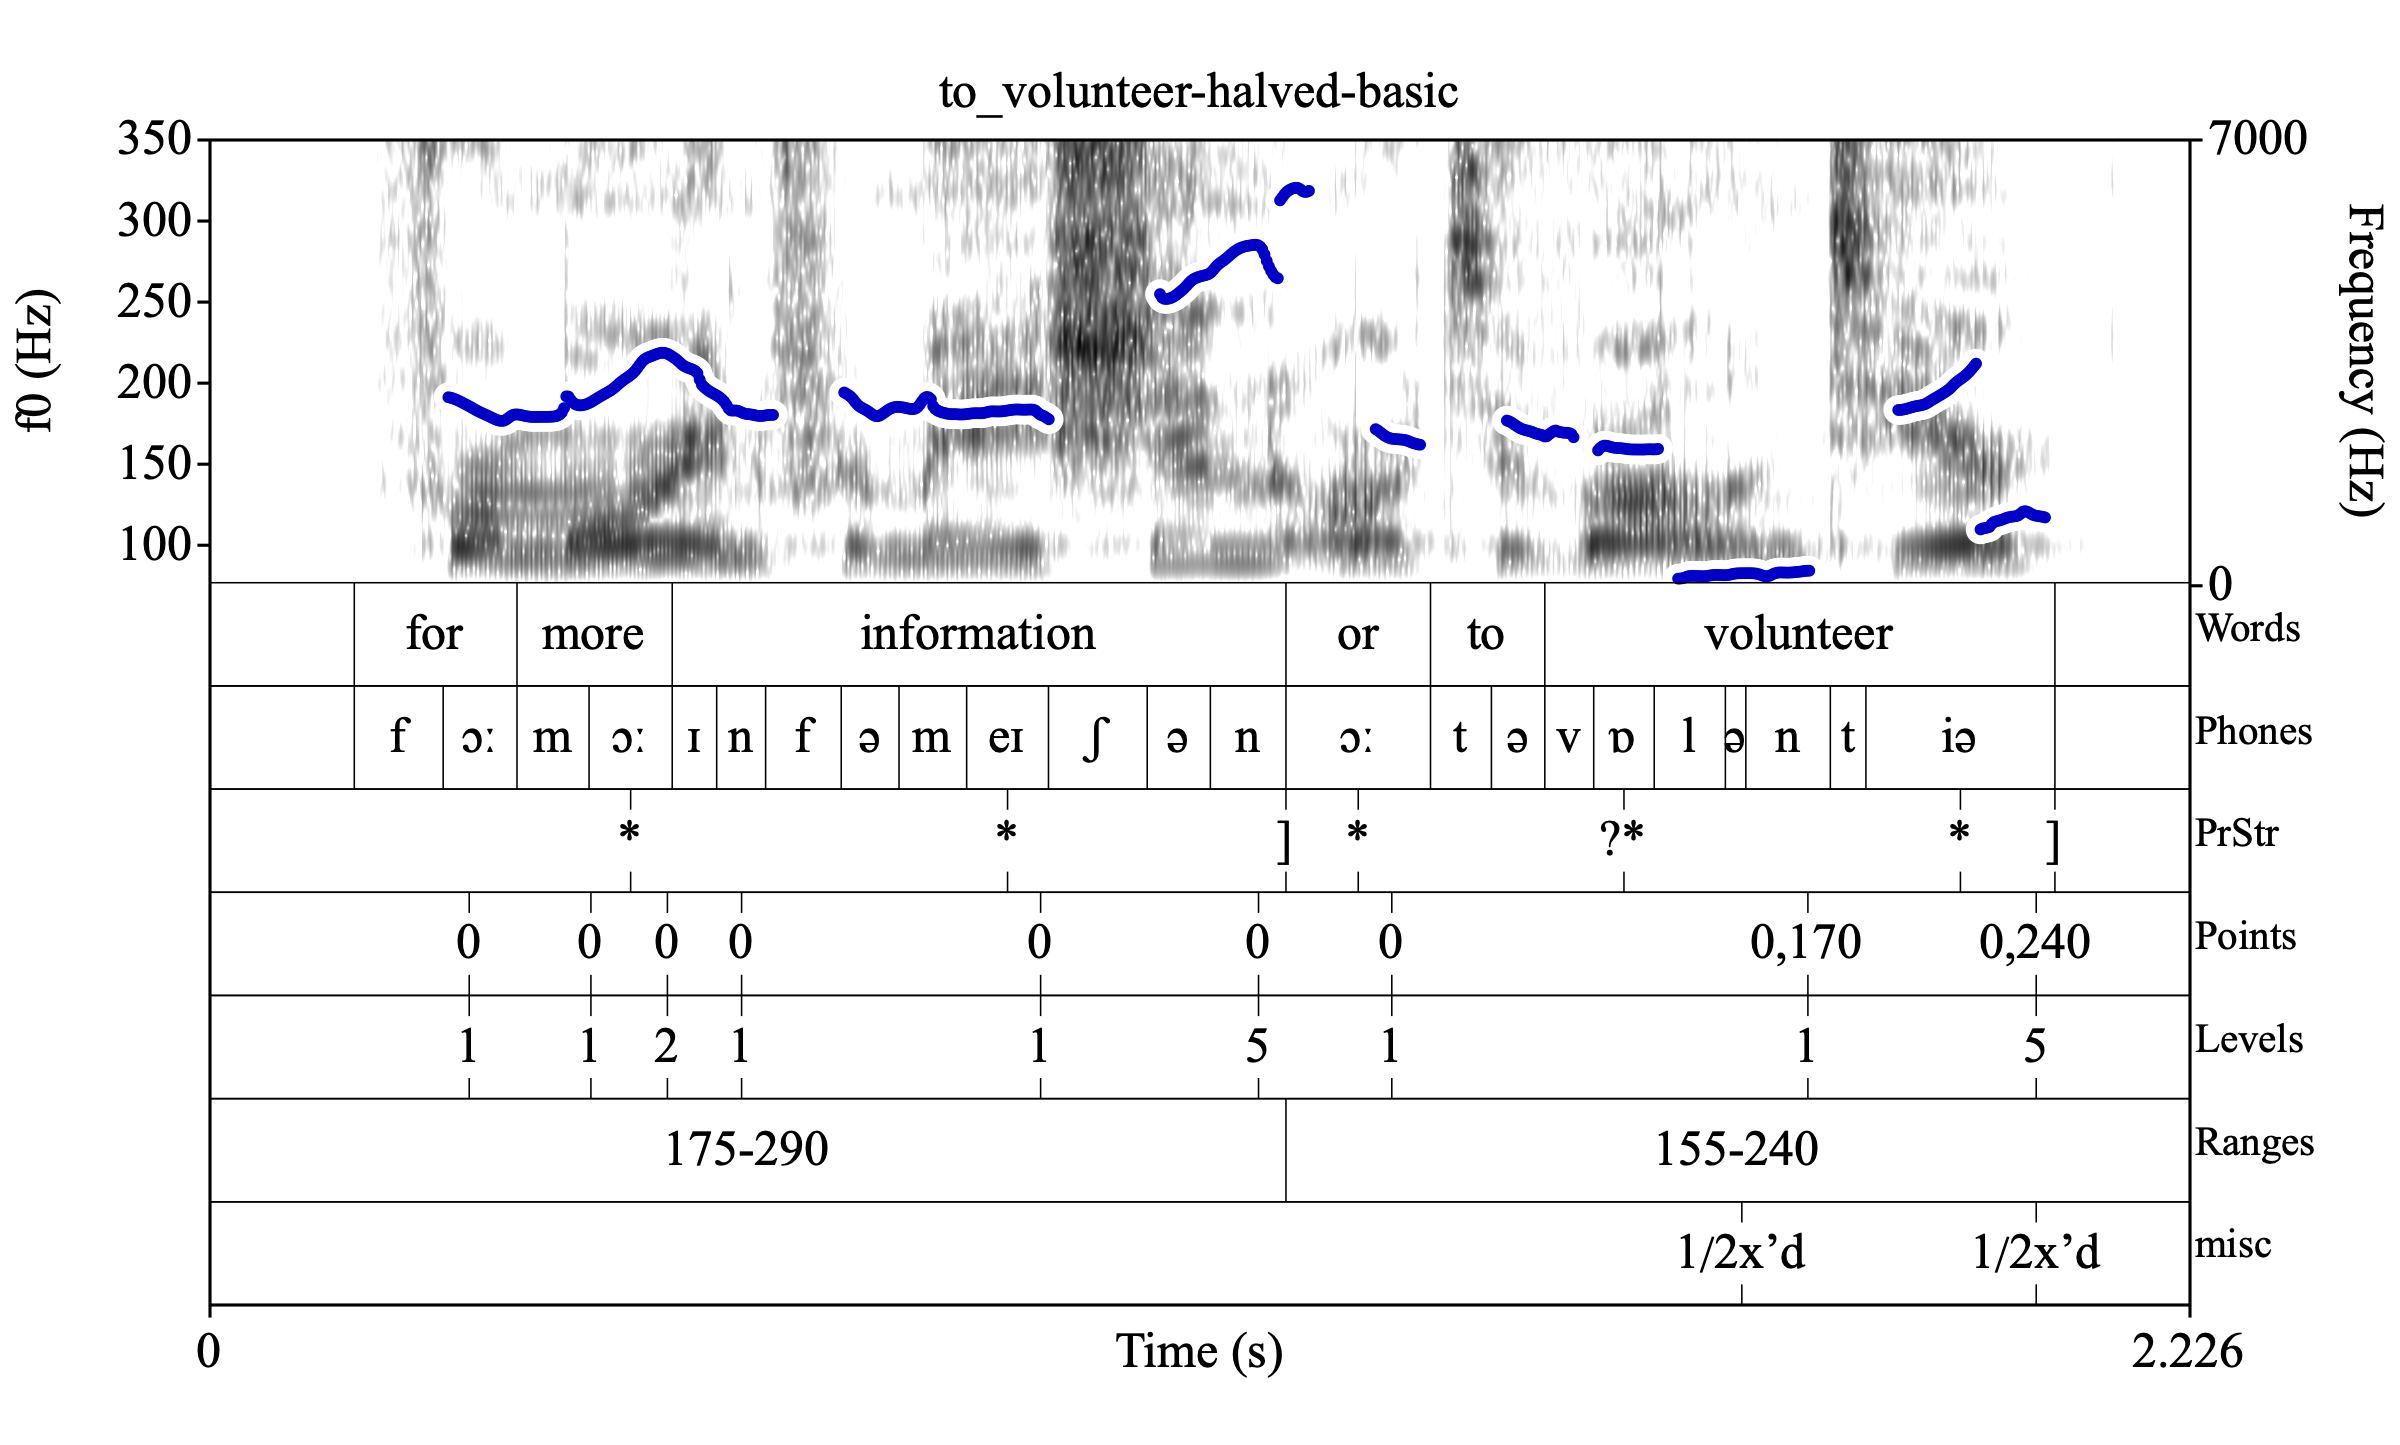
\includegraphics[width=.875\linewidth]{Appendix-to_volunteer-halved.png}
%
\caption{\texttt{to\_volunteer-halved}: An example annotated with PoLaR’s Basic labels.%
\label{fig:to volunteer-halved all basics}%
}
\end{figure}

There is no way to annotate this using PoLaR’s Basic labels, but this is the sort of thing the PoLaR Advanced labelling conventions (described in this chapter) have been designed for. Exactly how this and other analytical moves get transcribed using PoLaR Advanced labels will be described in the sections that follow.

While PoLaR Basic labels are designed to elicit agreement (even among labellers with different backgrounds in prosodic theory), Advanced labels may require labellers to have shared theoretical\slash analytical priors, in order for agreement to be reached. The PoLaR annotation system itself is not designed to provide answers that can adjudicate in these discussions, but rather it is meant to provide a starting point for these discussions to take place.

Before moving on, let us be clear about the optionality of using PoLaR Advanced labels. As described briefly above, PoLaR Advanced labels serve as a means to systematically encode higher levels of analysis or deeper intuitions that the labeller wishes to commit to. While other annotation systems require such higher-level commitments in most\slash all of their labels, PoLaR Advanced labels are always opt-in. This means that in cases where the labeller does not wish to commit to a particular analysis, they are not required to do so. (In sum, mixing PoLaR Basic labels with Advanced labels is both expected and encouraged, and researchers are encouraged to adopt the (sub)set of Advanced labels that best fits their research goals.)

\section{PoLaR Advanced Labels}\label{sec:polar-advanced-labels}

The sections that follow describe what we call PoLaR Advanced labels. These labels occupy the same four core PoLaR tiers (PrStr, Points, Levels, Ranges), but can encode more of the analyses and intuitions of advanced labellers, allowing for the annotation of relationships across tiers and for the inclusion of ideas informed by prosodic theories. In addition, these labels may be especially useful for describing data beyond idealized forms of mainstream varieties of a language produced in a laboratory setting.

Because these labels allow for inclusion of particular analyses, this chapter will have more discussion of how PoLaR labels can connect with prosodic theories and phonological analyses, and also how PoLaR fits in with / compares to existing annotation systems, especially those in the AM tradition. (See also \citealt{ahn-19}.)

A note before introducing these new PoLaR labels: Even with the addition of Advanced labels, these guidelines will \uline{not} provide an exhaustive set of labels that could be used in PoLaR. Labellers are encouraged to take advantage of PoLaR’s flexibility, by augmenting or changing the labels to fit their needs\slash views. However, whenever labellers do deviate from the descriptions set out in these guidelines, they need to provide a document that defines the labels they do use, providing descriptions that are at least as clear as those found in these guidelines (preferably with figures showing examples), so that other users have an explicit understanding of how those labels work.

\section{PrStr (Advanced)}\label{sec:prstr-advanced}

In the PrStr tier, phonological objects related to prominence and phrasing are annotated. In the Basic set of labels, the relevant labels are \textlabel{*} and \textlabel{]} (and their “uncertain” partners, \textlabel{?*} and \textlabel{?]}). One of the ideas behind reducing the number of necessary labels to \textlabel{*} and \textlabel{]} is to simplify the labelling process, allowing even untrained native speakers to provide such labels, in the spirit of Cole’s Rapid Prosody Transcription (\citealt{cole-14}). At the same time, it may be desirable (depending on the demands of the research at hand, and the abilities of the labeller(s)) to provide more detailed intuitions, beyond simply indicating the existence of prominence and phrase boundaries. To serve this need, this section will provide an expanded set of labels for the Prosodic Structure tier, for those who wish to include additional information about prominence and phrasing.

\subsection{Advanced Phrasing Labels}\label{sec:advanced-phrasing-labels}

A key component of any prosodic analysis is an understanding that there are a number of levels of hierarchical structure. English is commonly thought to make use of two phonologically distinct categories of prosodic phrasing (e.g., \citealt{selkirk81}, \citealt{beckmanpierrehumbert86}, \citealt{nesporvogel86}, \textit{et seqq}.), with evidence for such a distinction being rooted in different sorts of boundary phenomena (having to do with pitch movements, speech rate, pauses, pitch reset, etc.; \citealt{brugos-19}). As such, an advanced labeller may wish to distinguish some phrase boundaries from other phrase boundaries that are stronger. Thus in addition to the default \textlabel{]} label, PoLaR provides the \textlabel{]]} label for phrase boundaries that are perceived as stronger than others.

\begin{figure}[H]
\centering
%
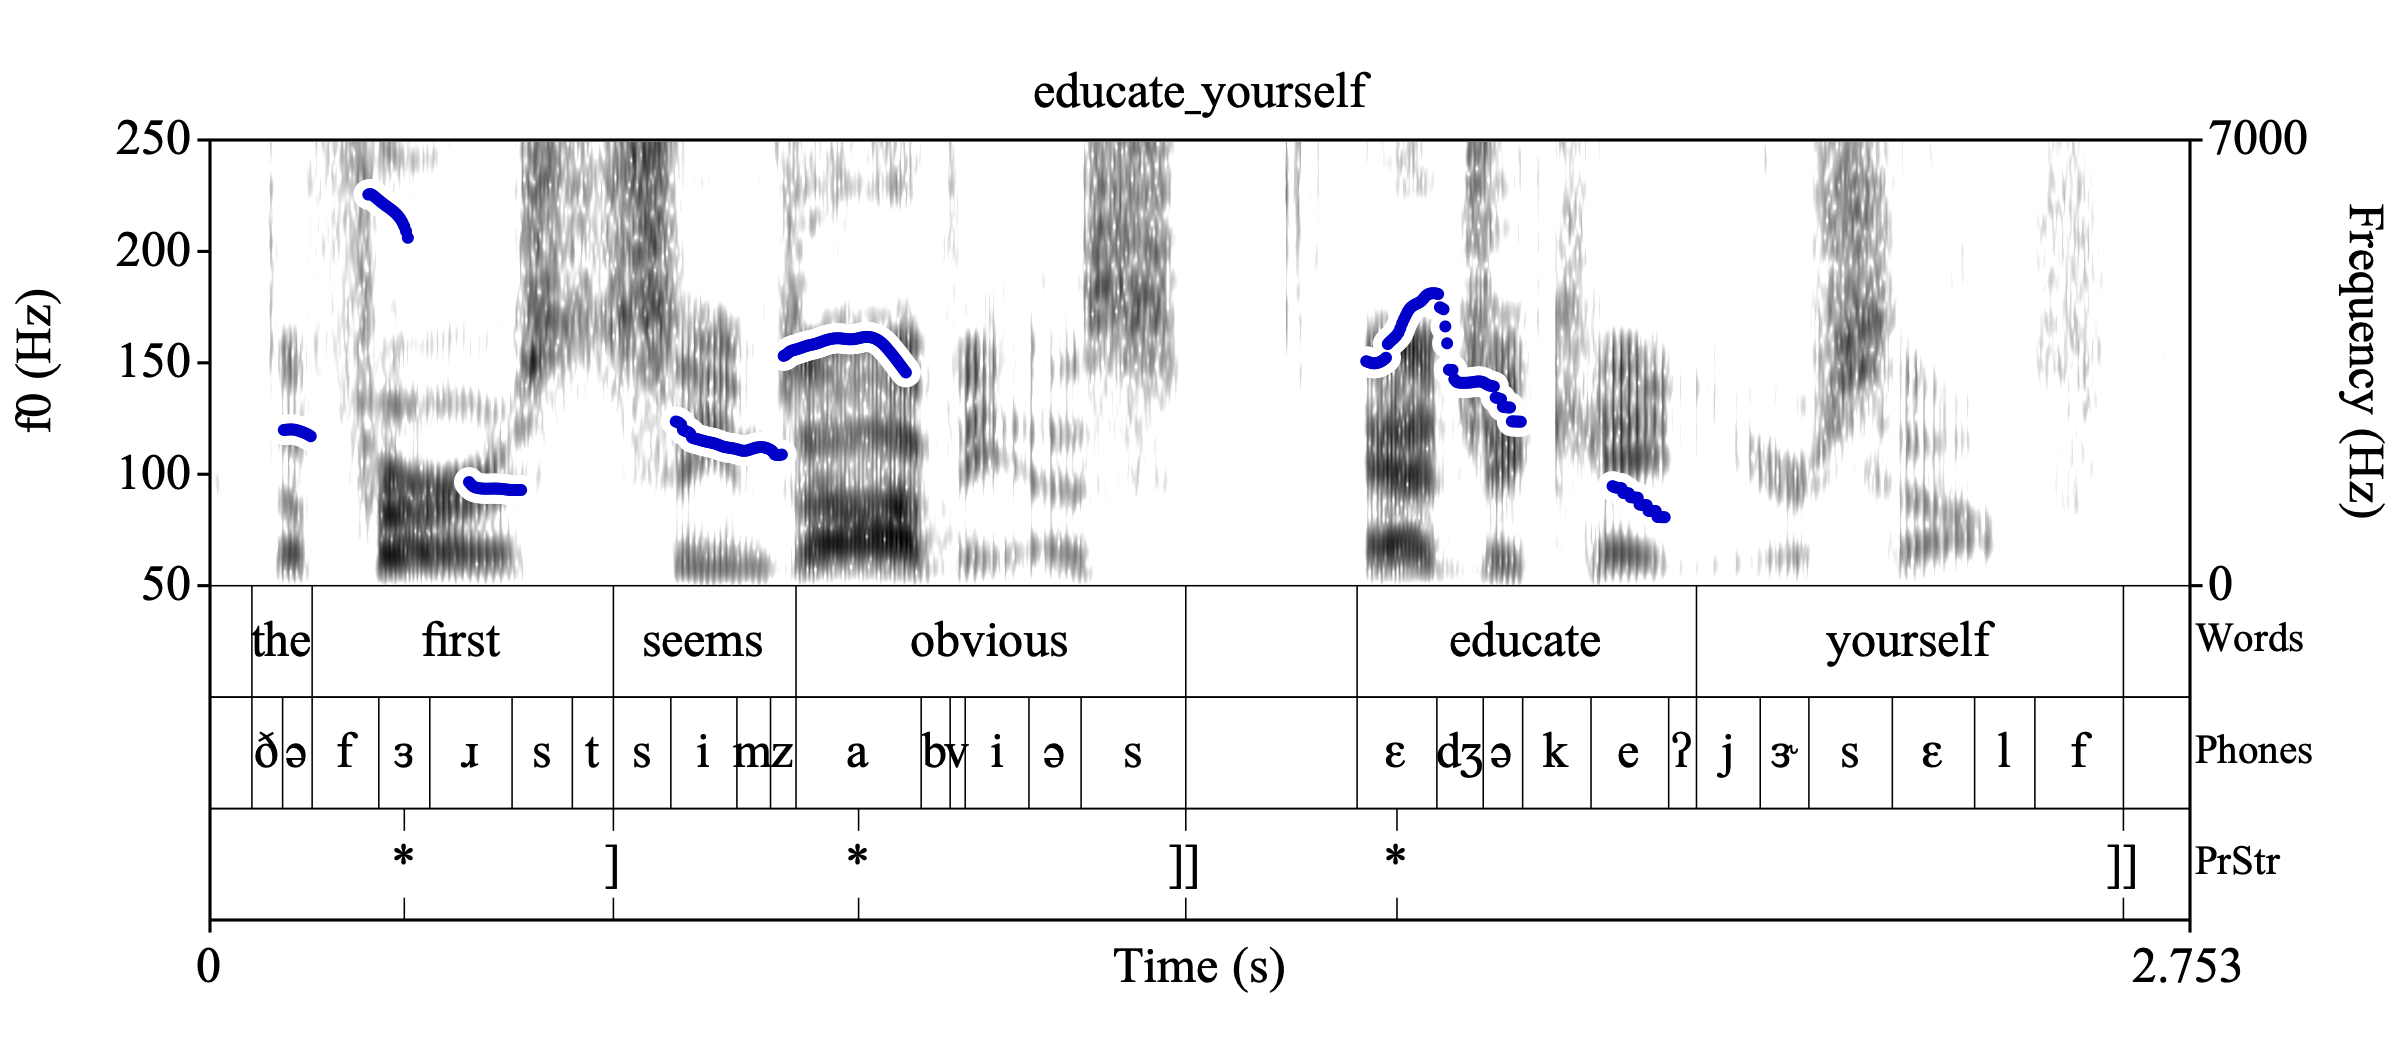
\includegraphics[width=.875\linewidth]{PrStr-educate_yourself-adv.png}
%
\caption{The labeller hears the phrase boundary between “\langtext{obvious}” and “\langtext{educate}” as stronger than the phrase boundary between “\langtext{first}” and “\langtext{seems}”.%
\label{fig:educate yourself PrStr Adv}%
\index{Annotated example, PrStr tier (advanced)!educate\_yourself}
}
\end{figure}

PoLaR does not require the labeller to adhere to any particular rigorous definitions for different sorts of prosodic phrases, across recordings. It may simply be that a labeller wishes to distinguish different levels of phrase-sizes in a particular example (perhaps due to their intuitive perception of disjuncture, or perhaps because some acoustic cue such as length of pause is particularly strong). Though labellers need not adhere to any particular rules on when to use \textlabel{]} versus {]]}, labellers may find it helpful to annotate in a “misc” tier what makes a \textlabel{]]} phrase boundary stand out as especially perceptually strong.

\subsubsection{Phrase-Initial Boundaries}\label{sec:phrase-initial-boundaries}

In addition to different sorts of phrase-final boundaries, a labeller may wish to also label the left edges of phrases, by using parallel labels like \textlabel{[}, \textlabel{?[}, and \textlabel{[[}. This may be useful if operating under an approach in which not every right edge of an intonation phrase entails the left edge of another intonation phrase. Because the Strict Layer Hypothesis (cf. \citealt{nesporvogel86}) in effect \textit{prohibits} recursion in prosodic structure, annotating a right edge is essentially annotating a left edge. However, many strands of contemporary research \textit{allow} recursion in prosodic structure (e.g., \citealt{ladd08}, \citealt{selkirk11}, \citealt{itomester12}, and \citealt{kentnerfery13}), making it useful to annotate both left and right edges of a phrase. For example, in a case of center-embedding like in “\langtext{I saw the lion \uline{which he loves} in the toy box}” with the non-restrictive relative clause, some may analyze the phrasing as “(\langtext{I saw the lion} (\langtext{which he loves}) \langtext{in the toy box})” – i.e., there is a phrase-initial edge before \langtext{which} but no phrase-final edge after \langtext{lion}. This could be annotated using Advanced phrasing labels as in Figure \ref{fig:lion toy box PrStr Adv}.

\begin{figure}[H]
\centering
%
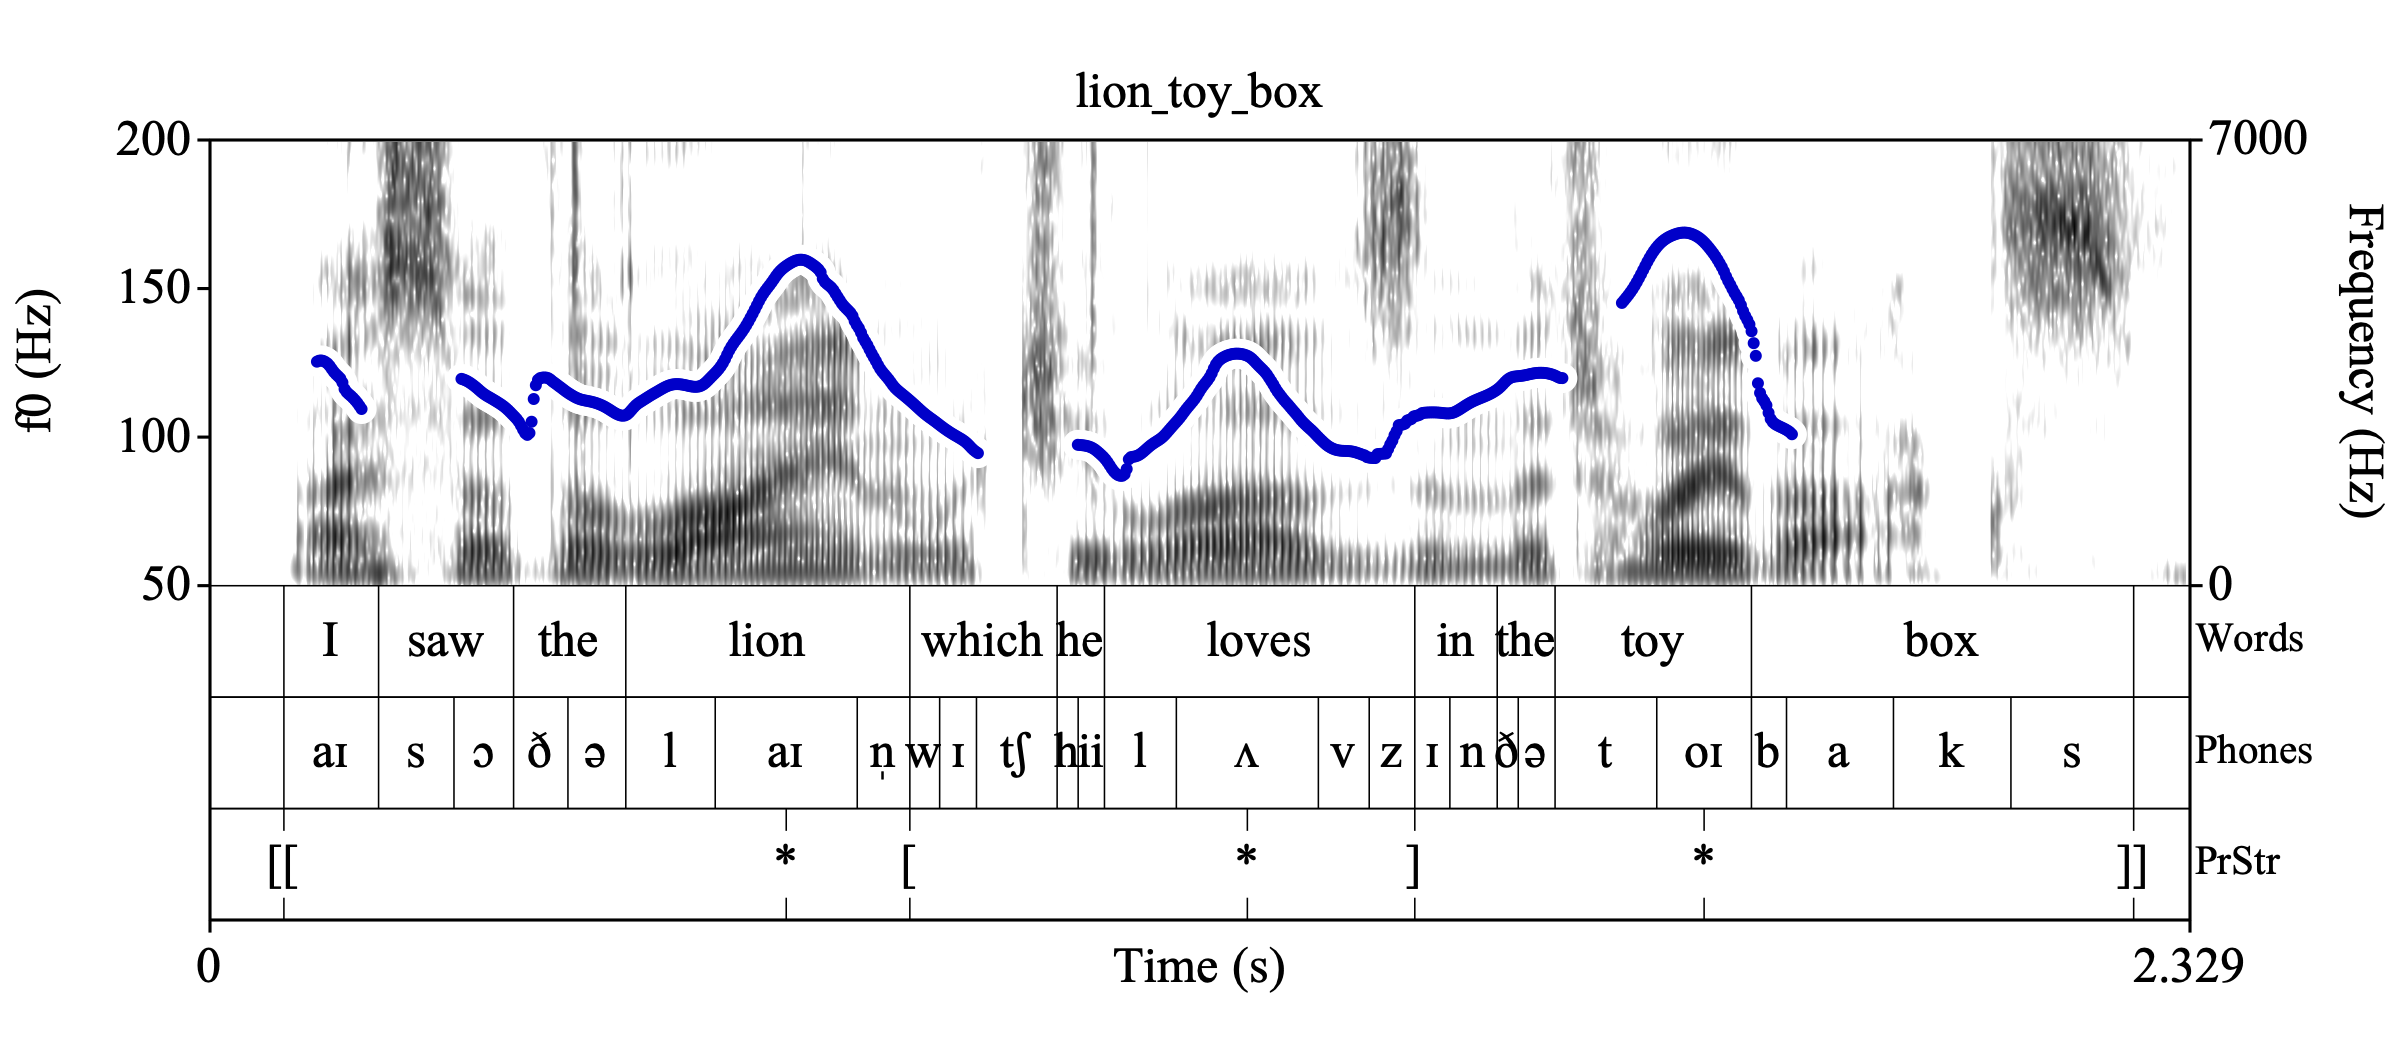
\includegraphics[width=.875\linewidth]{PrStr-lion_toy_box-adv.png}
%
\caption{The labeller is annotating an analysis in which “\langtext{lion}” is not phrase-final, even though “\langtext{which}” is phrase-initial.%
\label{fig:lion toy box PrStr Adv}%
\index{Annotated example, PrStr tier (advanced)!lion\_toy\_box}
}
\end{figure}

Similarly, with parentheticals that are produced like “\langtext{I think}” in Figure \ref{fig:long-story-ranges PrStr Adv}, there are cues to “\langtext{I}” being phrase-initial (glottalization), but not many cues to “\langtext{selling}” being phrase final. This could be analyzed in terms of nested prosodic phrases, and such an analysis is labelled on the PrStr tier in that figure.

\begin{figure}[H]
\centering
%
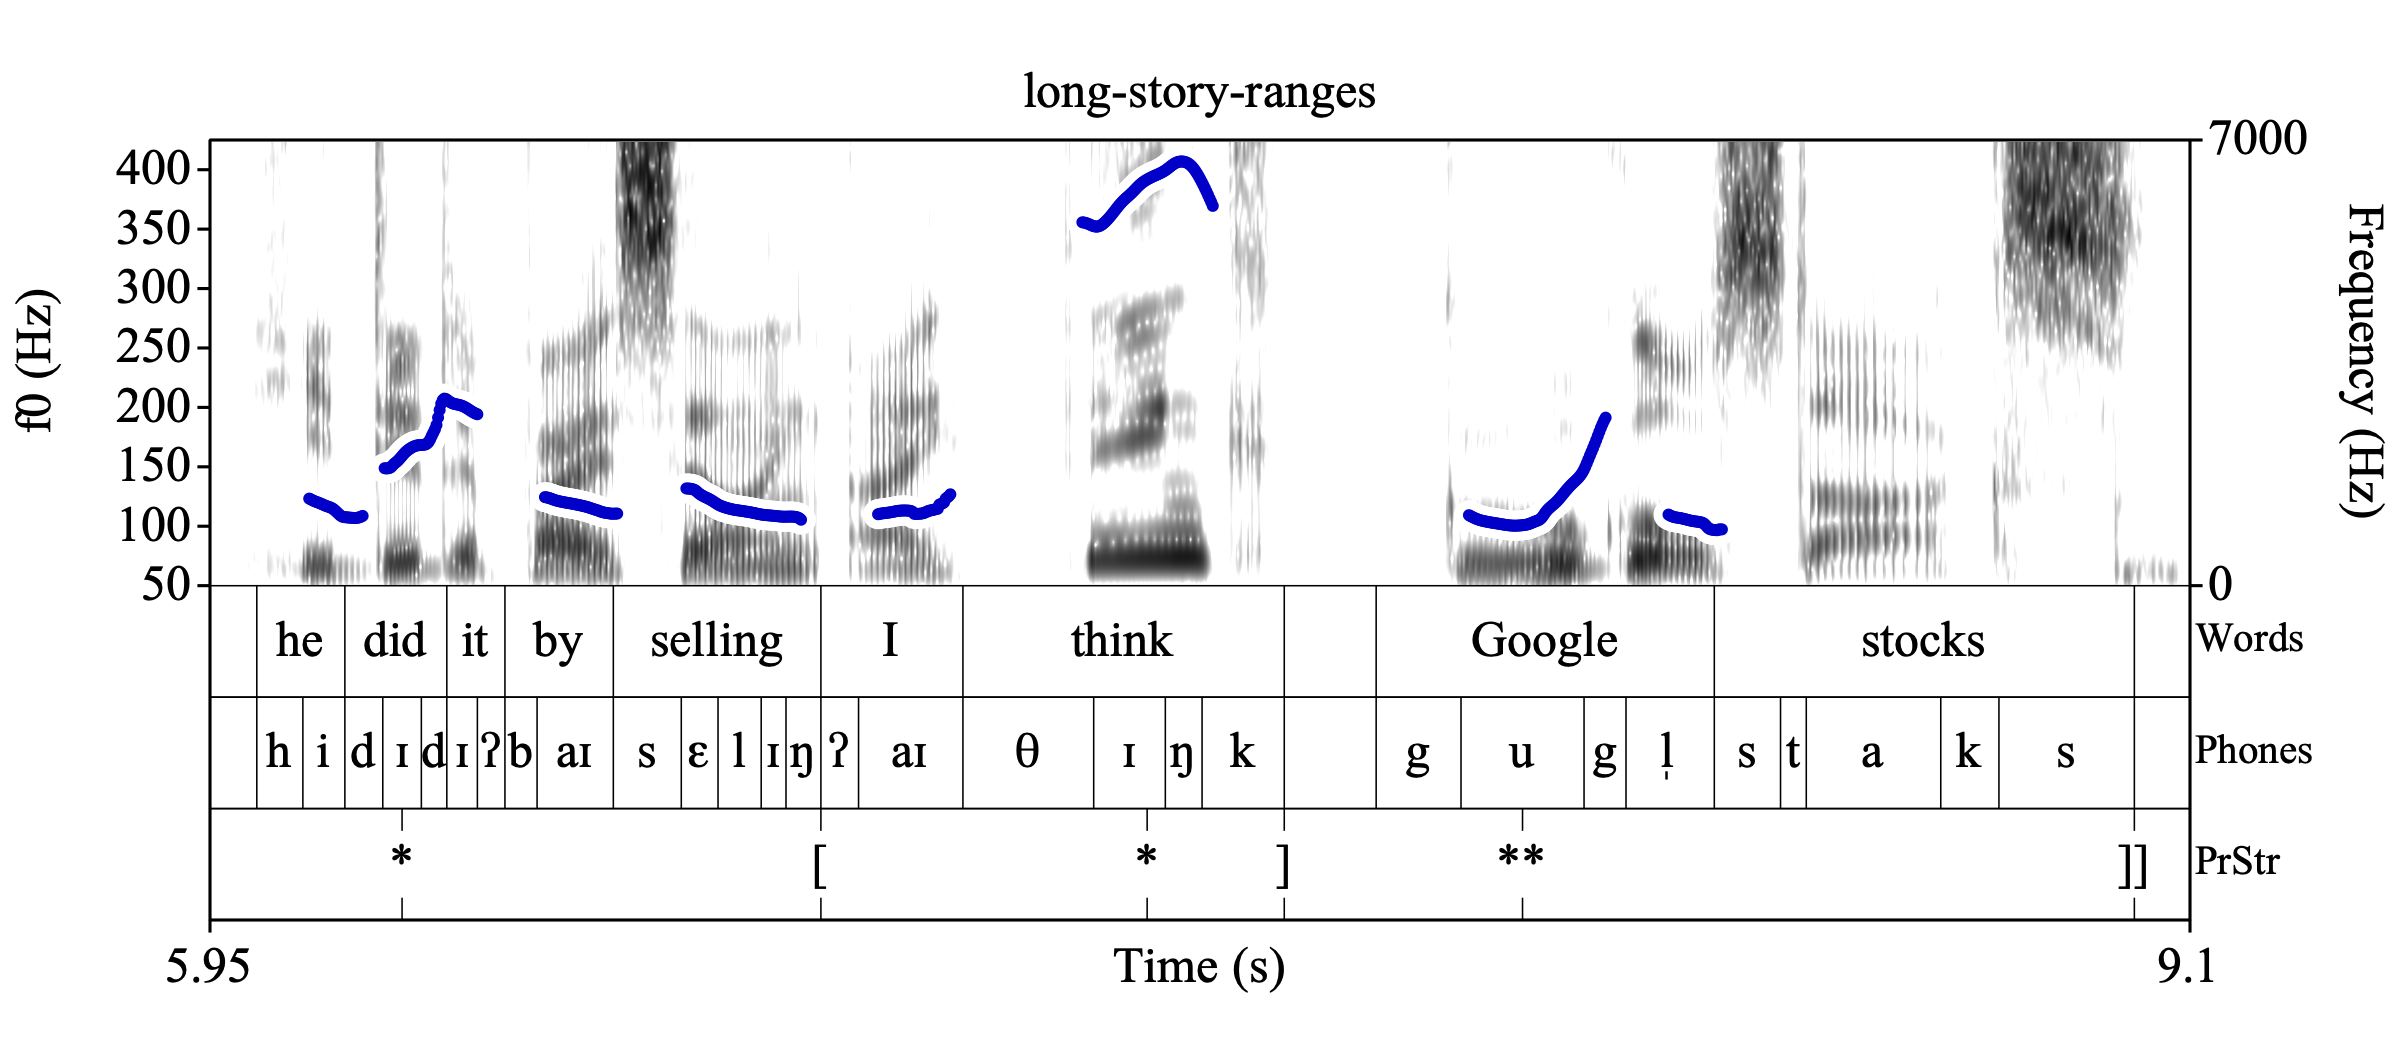
\includegraphics[width=.875\linewidth]{PrStr-long-story-ranges-adv.png}
%
\caption{The labeller is annotating an analysis in which “\langtext{selling}” is not phrase-final, just because “\langtext{I}” is phrase-initial.%
\label{fig:long-story-ranges PrStr Adv}%
\index{Annotated example, PrStr tier (advanced)!long-story-ranges}
}
\end{figure}

For researchers who choose to label phrase beginnings with the \textlabel{[} label, there may be occasions where a single word boundary coincides with both the end of one phrase and the beginning of another, with no intervening silent interval. It is possible to use \textlabel{][} at such points, as is illustrated in Figure \ref{fig:vegetable_list PrStr Adv} below:

\begin{figure}[H]
\centering
%
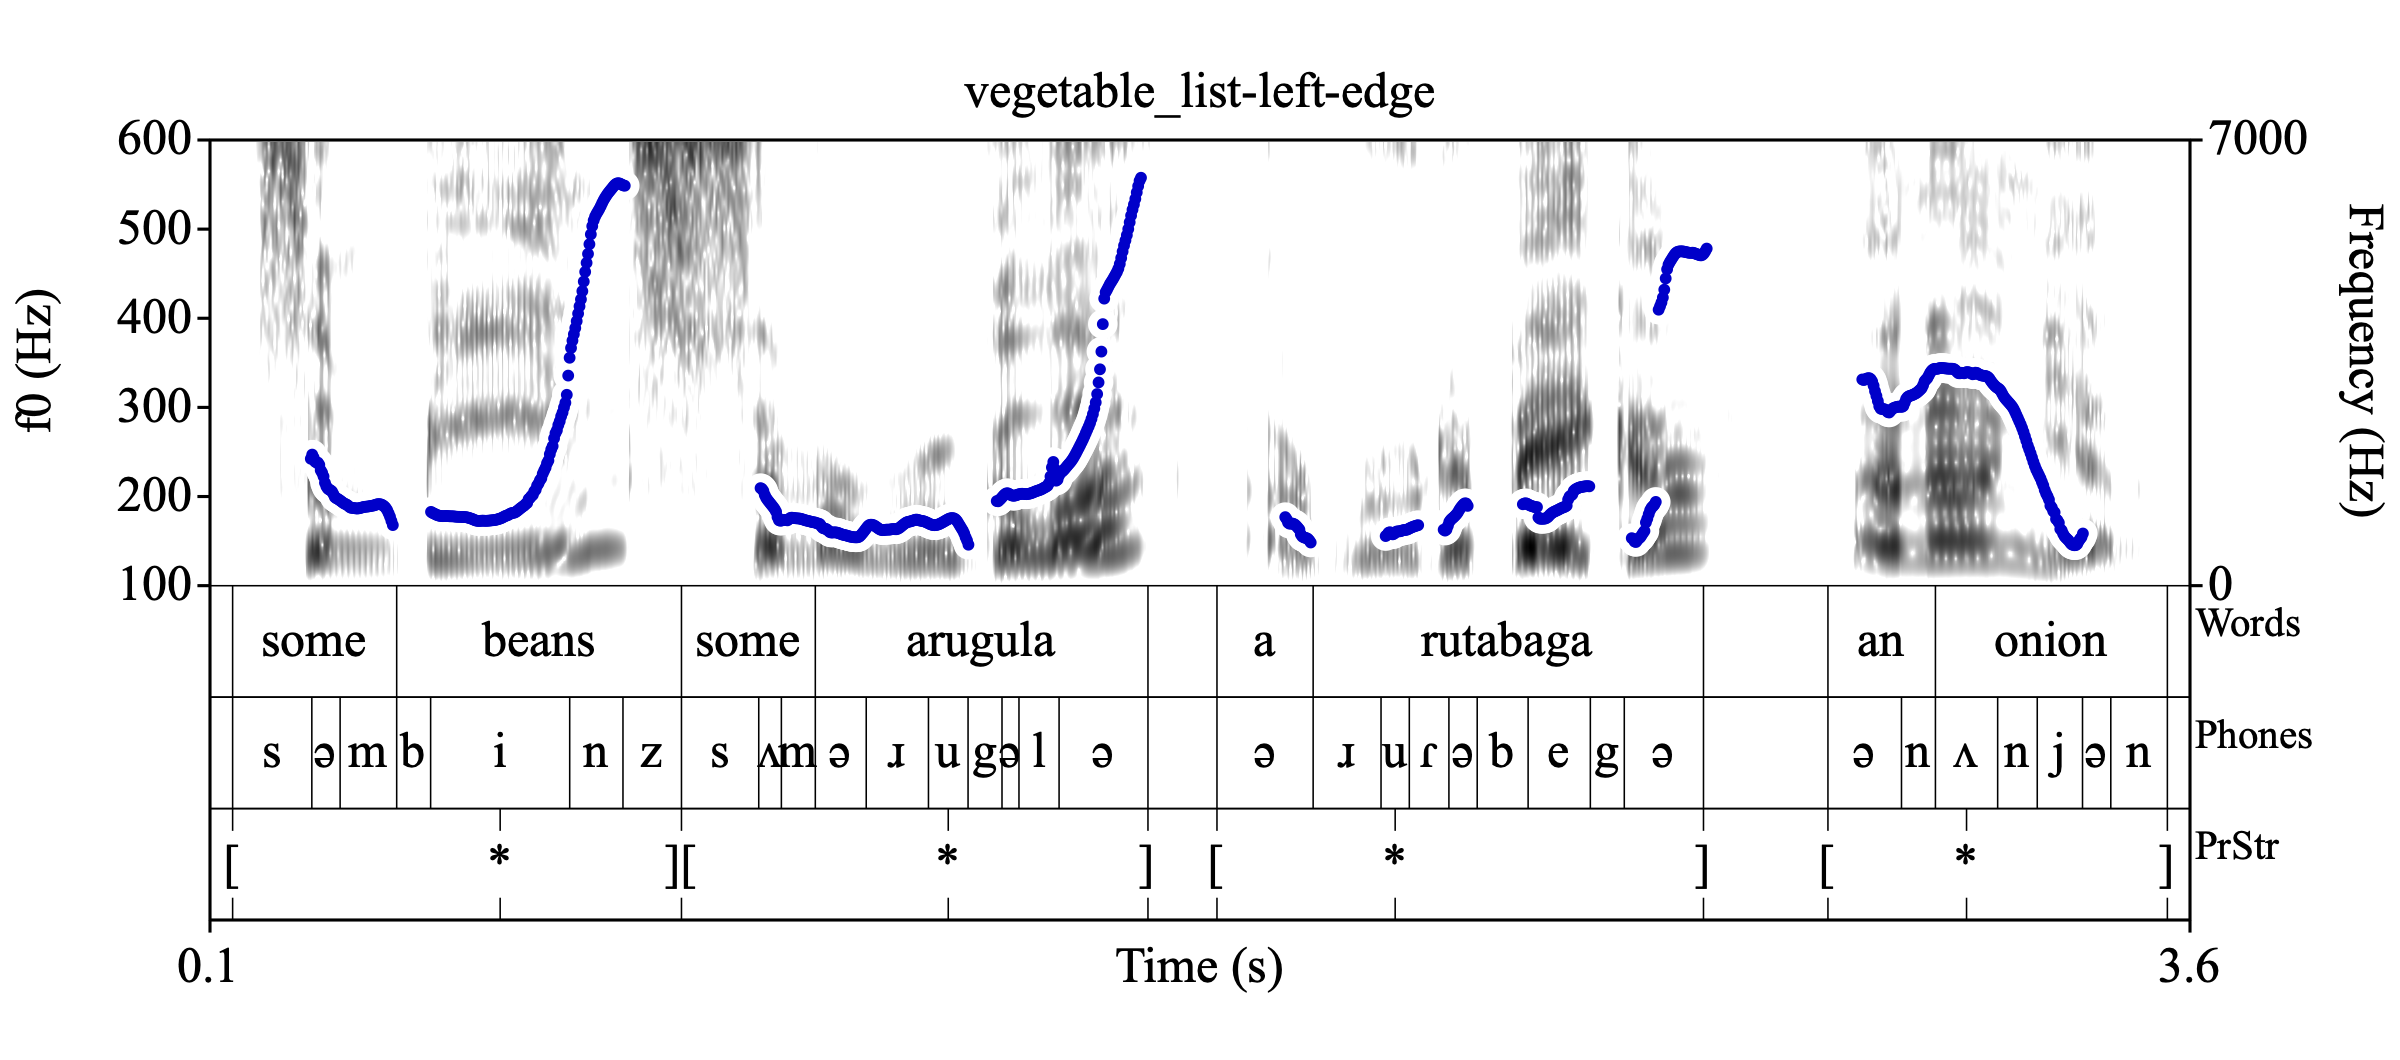
\includegraphics[width=.875\linewidth]{PrStr-vegetable_list-adv.png}
%
\caption[The labeller has annotated the beginning of each phrase as well as its end.]{The labeller has annotated the beginning of each phrase as well as its end, including an instance of the same location being both a phrase end and a phrase beginning, i.e. the marker between “\langtext{beans}” and “\langtext{some}.”%
\label{fig:vegetable_list PrStr Adv}%
\index{Annotated example, PrStr tier (advanced)!vegetable\_list}
}
\end{figure}

Note that we offer this \textlabel{[} label as a tool for those who would find using it to be helpful for their research purposes, and using it is by no means required. In other words, use the \textlabel{[} label if you are compelled to, but we take no stance on how often labellers should be using it (if at all). For some cases where \textlabel{[} labels may be useful for Advanced Points labels, see section \ref{sec:points-associated-with-phrase-initial-boundaries}.

\subsubsection{Summary of Phrasing Labels}\label{sec:summary-of-phrasing-labels}

Basic labels are highlighted, to be used by all, with the remaining Advanced labels provided for labellers who have more experience or who are targeting particular phenomena. As a reminder: phrasing is cued by acoustics, but these labels are about the labeller’s \textit{perception} or phrasing, in the given utterance context.

\begin{longtable}{clp{.5\linewidth}} \toprule \textbf{Label} & \textbf{Phonological Object} & \textbf{Significance of Label}\tabularnewline
\midrule \endhead
\rowcolor{green}
\textlabel{]} & Prosodic Phrase Boundary & A prosodic phrase ends at this point \tabularnewline
\textlabel{?]} & Possible Prosodic Phrase Boundary & A prosodic phrase may end at this point, but the labeller is uncertain \tabularnewline
\textlabel{]]} & Large Prosodic Phrase Boundary & A noticeably large prosodic phrase ends at this point \tabularnewline
\textlabel{[} & Prosodic Phrase Boundary & A prosodic phrase begins at this point \tabularnewline
\textlabel{?[} & Possible Prosodic Phrase Boundary & A prosodic phrase may begin at this point, but the labeller is uncertain \tabularnewline
\textlabel{[[} & Large Prosodic Phrase Boundary & A noticeably large prosodic phrase begins at this point \tabularnewline
%
\bottomrule
\caption{Advanced PrStr phrasing labels: encoding uncertainty or boundary strength.}
\end{longtable}

\subsection{Advanced Prominence Labels}\label{sec:advanced-prominence-labels}

Just as there are levels of prosodic phrasing, in some cases different levels of prosodic prominence can be identified perceptually and/or acoustically. In such cases an advanced labeller may wish to distinguish some prominences from other prominences that are stronger. Thus in addition to the default \textlabel{*} label, PoLaR provides the \textlabel{**} label for prominences that are perceived as stronger than others.

\begin{figure}[H]
\centering
%
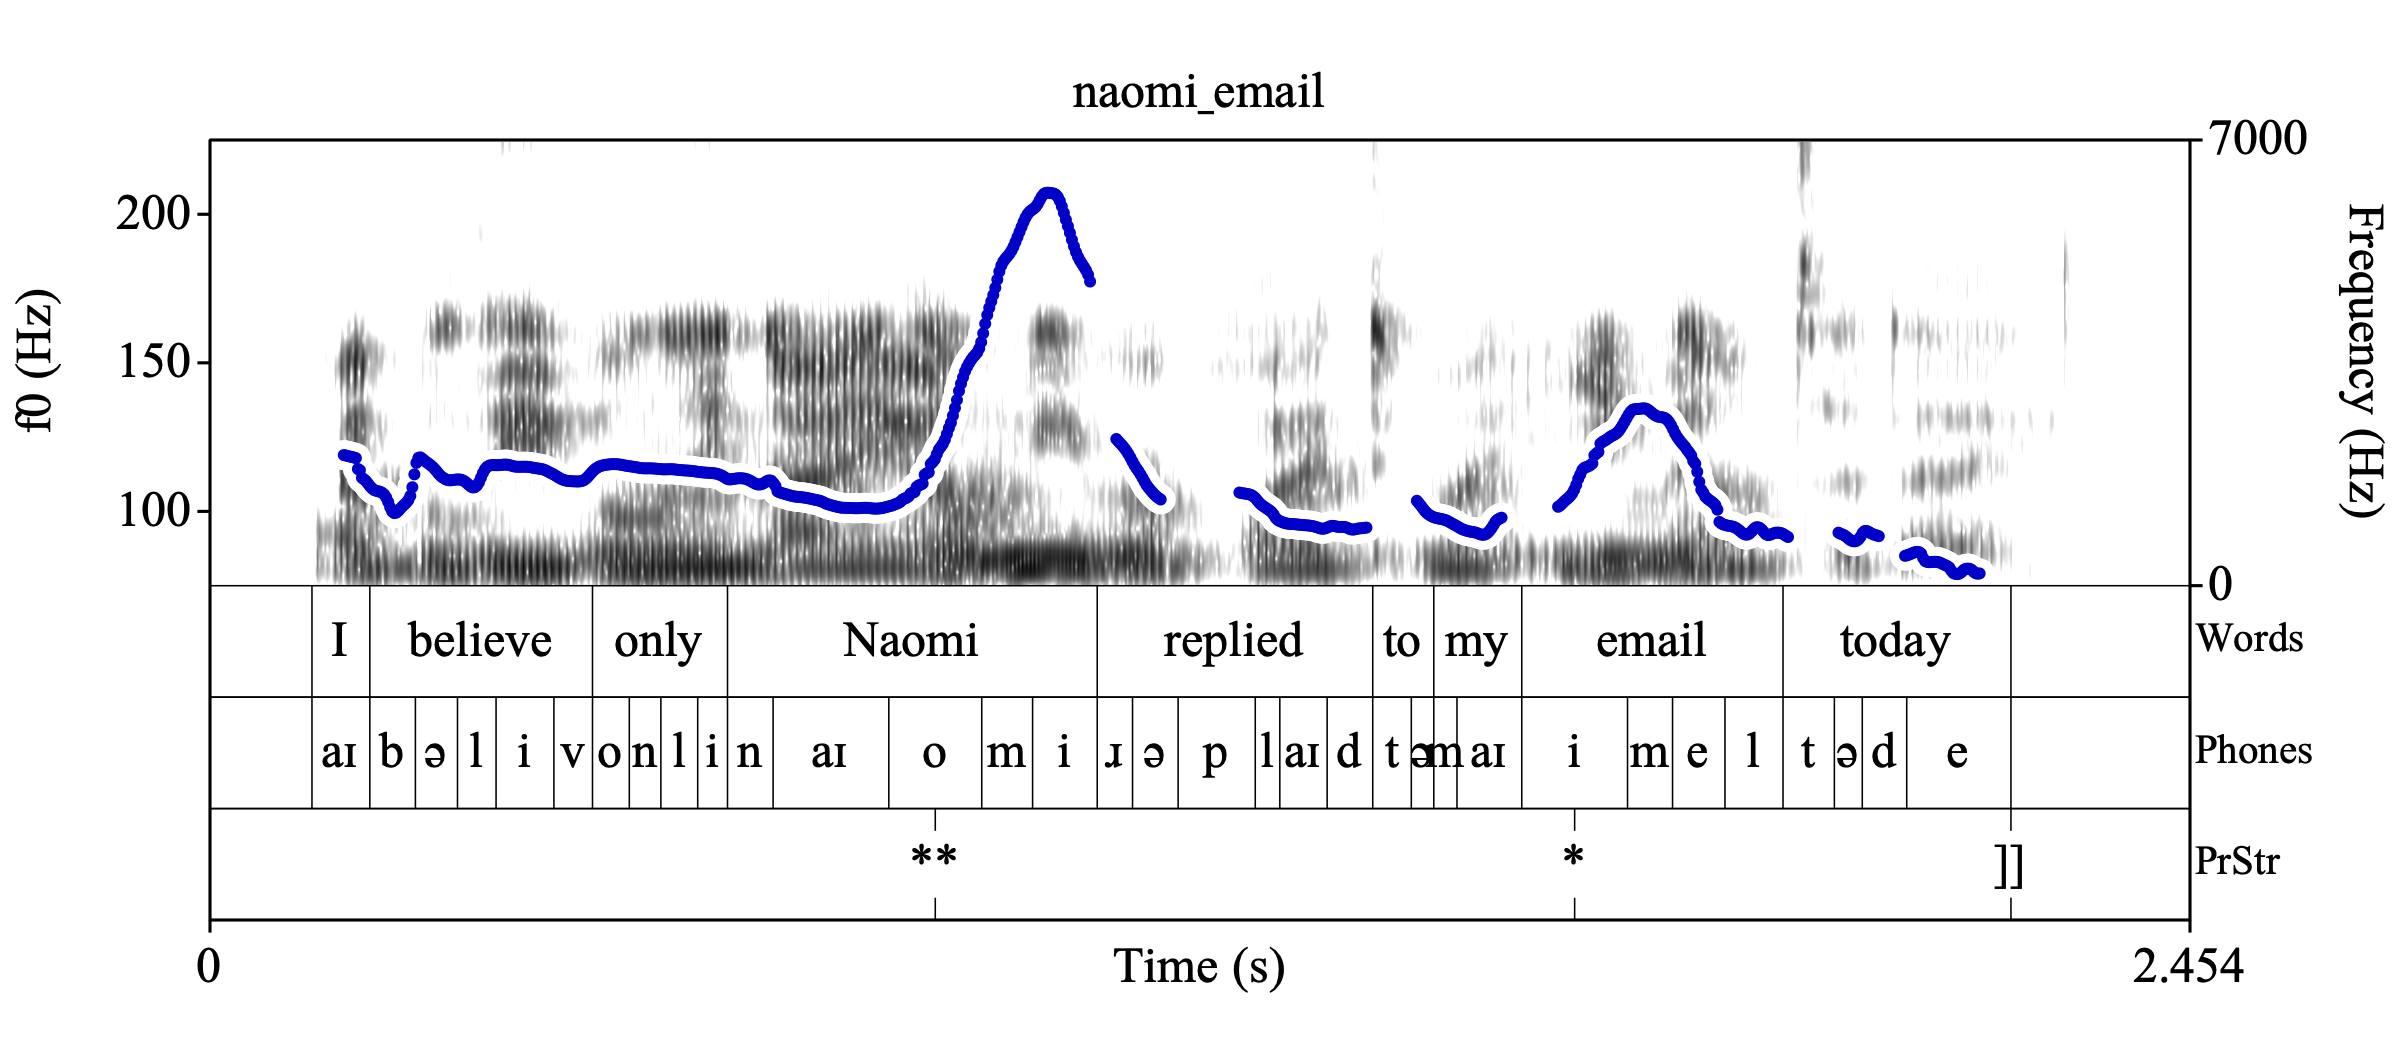
\includegraphics[width=.875\linewidth]{PrStr-naomi_email-adv.png}
%
\caption{The labeller is annotating the perception that “\langtext{Naomi}” and “\langtext{email}” are both prominent, but that “\langtext{Naomi}” is significantly more prominent.%
\label{fig:naomi_email PrStr Adv}%
\index{Annotated example, PrStr tier (advanced)!naomi\_email}
}
\end{figure}


As with all Advanced labels, there is no need to use \textlabel{**} in every utterance. As default guidance for distinguishing \textlabel{*} and \textlabel{**}, labellers should only use the \textlabel{**} label when it is very clear that one of the prominences is perceived as especially strong, as compared to the other words in the context of the utterance.

Additionally, as with the \textlabel{]} and \textlabel{]]} labels, PoLaR does not require the labeller to adhere to any particular rigorous definitions for different sorts of prominence across their entire corpus; a labeller may simply wish to distinguish different degrees of prominence in a given example (perhaps as a simple matter of perceptual strength, perhaps because of especially high f0 peaks, etc.). That said, labellers are encouraged to annotate in a “misc” tier what makes a \textlabel{**} prominence stand out as especially perceptually strong.

\subsubsection{Summary of Prominence Labels}\label{sec:summary-of-prominence-labels}

Basic labels are highlighted, to be used by all, with the remaining labels proposed for labellers who have more experience or who are targeting particular phenomena. As a reminder: prominence is cued by acoustics, but these labels are about the labeller’s \textit{perception} or prominence, in the given utterance context.

\begin{longtable}{clp{.5\linewidth}} \toprule \textbf{Label} & \textbf{Phonological Object} & \textbf{Significance of Label}\tabularnewline
\midrule \endhead
\rowcolor{green}
\textlabel{*} & Prominence & The constituent this occurs in is prominent\tabularnewline
\textlabel{?*} & Possible Prominence & The constituent this occurs in might be prominent, but the labeller is uncertain \tabularnewline
\textlabel{**} & Especially Strong Prominence & The constituent this occurs in is especially prominent \tabularnewline
%
\bottomrule
\caption{Advanced PrStr prominence labels: encoding uncertainty or prominence strength.}
\end{longtable}

\subsection{Disfluency}\label{sec:disfluency}

Here we pivot from labelling phrasing and prominence to labelling a phenomenon that may interact with perceived phrasing\slash prominence: disfluencies in speech. A disfluency is defined here as a disruption of fluent, connected speech, which manifests acoustically as a change in speech rate, a change in pitch trajectory, addition of a pause, etc. Such an acoustic disruption can be momentary in nature, or it can be observed over a period of time. (See \citealt{shattuck-hufnagelcutler99} for a discussion of how different types of disfluency can be marked prosodically. In addition, \citealt{brugos-19} describes in more detail the range of disfluency effects on prosody that are attested in English.) Characteristic of all types of disfluencies is that, if a speaker were to repeat an idealized form of the disfluency-containing utterance, with the same intended meaning, the idealized repetition could lack all disfluent regions.

As disfluencies can influence prosody in measurable ways, a labeller may find it useful to label disfluent speech as such. For this purpose, PoLaR provides the ‘\textlabel{d}’ label, which is to be marked on the PrStr tier, at the point in the utterance where there is a disfluency: i.e., in the word or partial word (in the case of a cut-off word) where the disfluency is noticed.

While disfluencies may differ prosodically from one another, this ‘d’ label can be used for all types. An example of a disfluency that corresponds to a momentary stutter (with no sense of disjuncture) is given in Figure \ref{fig:in_a_plane-disfluencies PrStr Adv}. Additionally, an example of a disfluency that induces a sense of disjuncture like that of a phrase boundary (due to the overlap in set of cues) is given in Figure \ref{fig:spoon_here PrStr Adv}. In both cases, the ‘\textlabel{d}’ label is on the PrStr tier, time-aligned with the onset of the disfluent moment\slash region, or where the speaker cuts themselves off.

\begin{figure}[H]
\centering
%
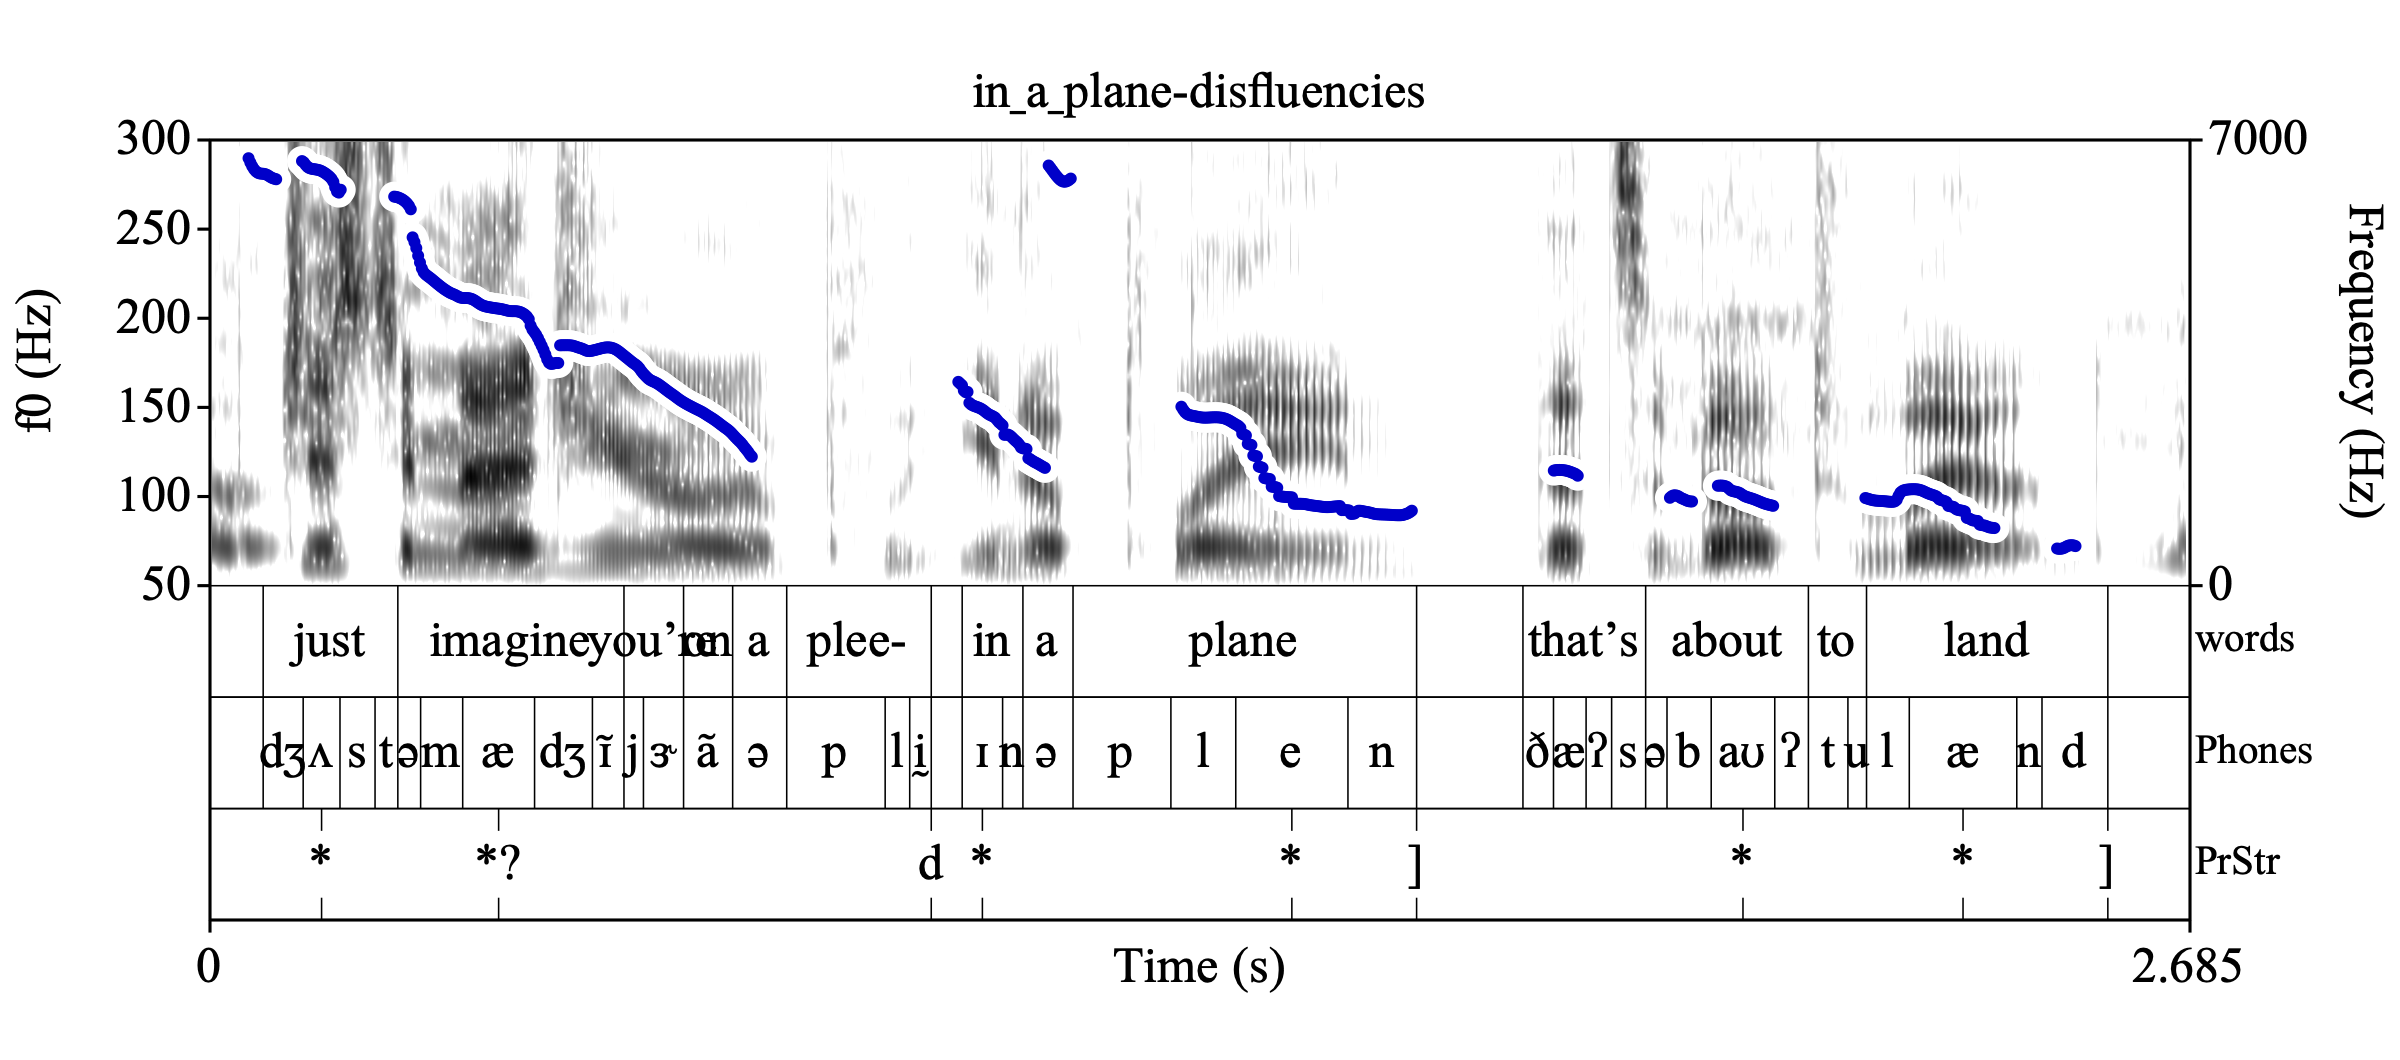
\includegraphics[width=.875\linewidth]{PrStr-in_a_plane-disfluencies-adv.png}
%
\caption[\texttt{in\_a\_plane-disfluencies}, with Advanced PoLaR labels.]{\texttt{in\_a\_plane-disfluencies}, with Advanced PoLaR labels. Note the ‘d’ on PrStr, annotating at the cut-off, before a restart begins.%
\label{fig:in_a_plane-disfluencies PrStr Adv}%
\index{Annotated example, PrStr tier (advanced)!in\_a\_plane-disfluencies}
}
\end{figure}

\begin{figure}[H]
\centering
%
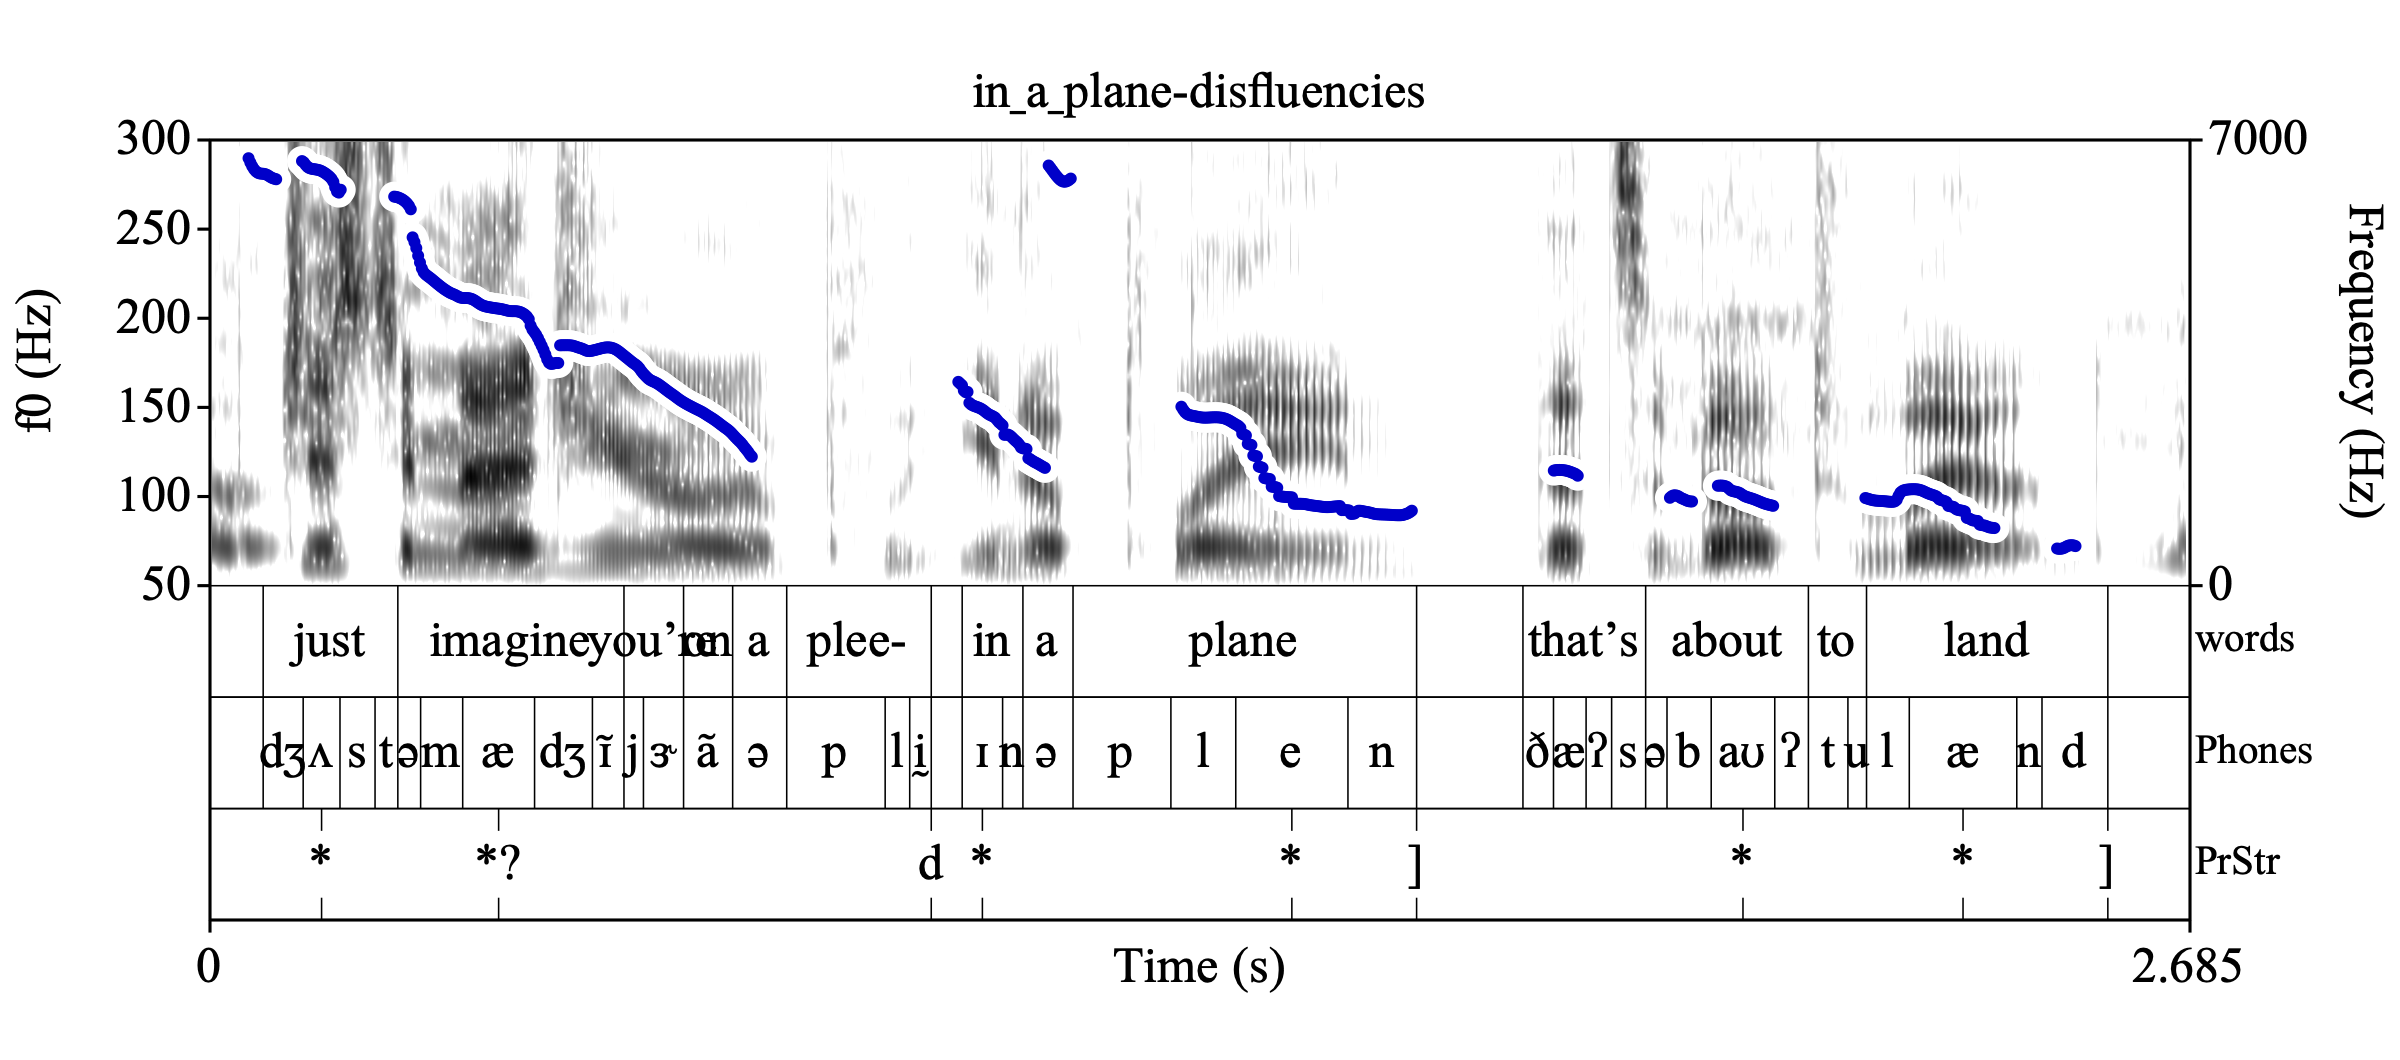
\includegraphics[width=.875\linewidth]{PrStr-in_a_plane-disfluencies-adv.png}
%
\caption[\texttt{spoon\_here}, with Advanced PoLaR labels. Note the ‘\textlabel{d}’ on PrStr.]{\texttt{spoon\_here}, with Advanced PoLaR labels. Note the ‘\textlabel{d}’ on PrStr, annotating where a labeller may perceive some of the prosody associated with this disfluency as cues to phrase break.%
\label{fig:spoon_here PrStr Adv}%
\index{Annotated example, PrStr tier (advanced)!spoon\_here}
}
\end{figure}

There may be cases in which a speaker produces not just a single disfluency, but a disfluent region. For such cases, the labeller can designate the beginning and ending of such a region by using the ‘\textlabel{\{d}’ and ‘\textlabel{d\}}’ labels in the PrStr tier at the beginning and end (respectively) of this region. The labeller can choose to skip over other labelling decisions within this designated region. Such an example is shown in Figure \ref{fig:experience-disfluent-region PrStr Adv}.

\begin{figure}[H]
\centering
%
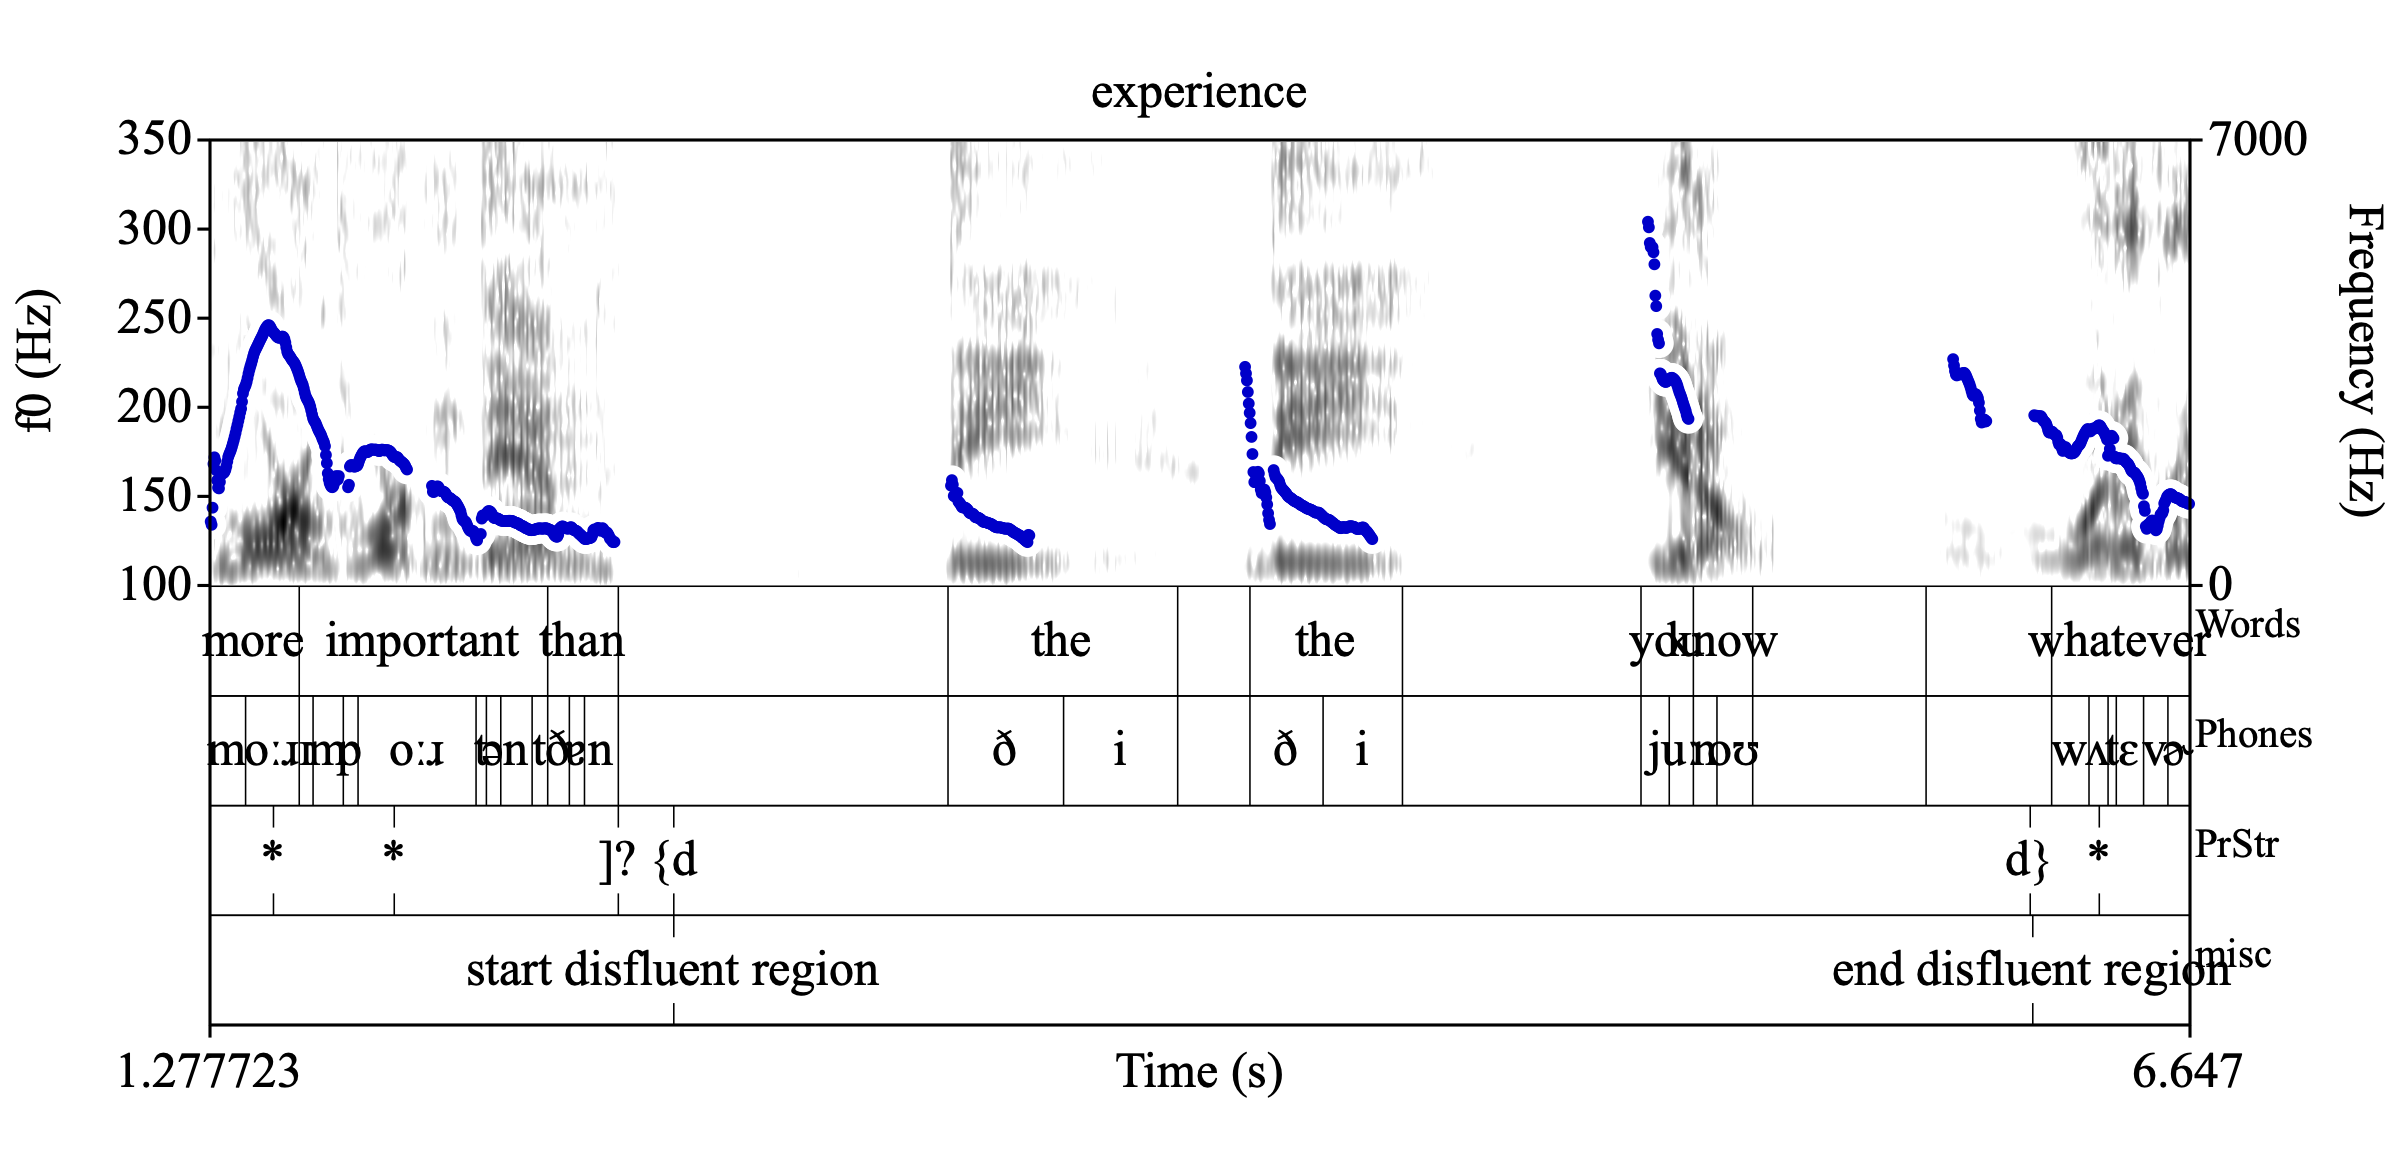
\includegraphics[width=.875\linewidth]{PrStr-experience-disfluent-region.png}
%
\caption[\texttt{experience}, with Advanced PoLaR labels. Note the region flanked by ‘\textlabel{\{d}’ and ‘\textlabel{d\}}’ on PrStr.]{\texttt{experience}, with Advanced PoLaR labels. Note the region flanked by ‘\textlabel{\{d}’ and ‘\textlabel{d\}}’ on PrStr, which annotate a stretch of time that sounds disfluent.%
\label{fig:experience-disfluent-region PrStr Adv}%
\index{Annotated example, PrStr tier (advanced)!experience}
}
\end{figure}

In all cases, the ‘\textlabel{d}’ label of PoLaR allows the labeller to annotate the presence of one or more disfluencies, without any information about the acoustic details or which (if any) type of speech error it corresponds to. Labellers who wish to label more about the details of the disfluency are encouraged to use a system of labels designed to annotate this information, perhaps on a different tier. (See \citealt{brugos-19} for some ideas of disfluency labels that could work alongside PoLaR.)

\begin{longtable}{cp{.3\linewidth}p{.45\linewidth}}
	\toprule
	\textbf{Label} & \textbf{Phonological Object} & \textbf{Time-Aligned with} \tabularnewline
	\midrule
	\endhead
	\textlabel{d} & Disfluency & A point in the utterance where there is a disfluency\tabularnewline
	\textlabel{\{d} & Start of a disfluent region & A point in the utterance where a disfluent region of speech begins\tabularnewline
	\textlabel{d\}} & End of a disfluent region & A point in the utterance where a disfluent region of speech ends\tabularnewline
	\bottomrule
	\caption{Advanced PrStr labels: encoding disfluency.}
\end{longtable}


\subsection{Examples with Advanced PrStr labels}\label{sec:examples-with-advanced-prstr-labels}

In this section we have reviewed some ways to systematically label these more refined intuitions, beyond the simple contrast of presence\slash absence of \textlabel{*} and \textlabel{]} labels; e.g., using the contrast between \textlabel{*} and \textlabel{**} labels, and \textlabel{]} and \textlabel{]]} labels to differentiate degrees of prominence\slash phrasing. In addition to the examples provided earlier in this section, these more fine-grained contrasts are exemplified in Figure \ref{fig:out_of_order_huh PrStr Adv} and Figure \ref{fig:asked_only_an_illusion PrStr Adv}.

\begin{figure}[H]
\centering
%
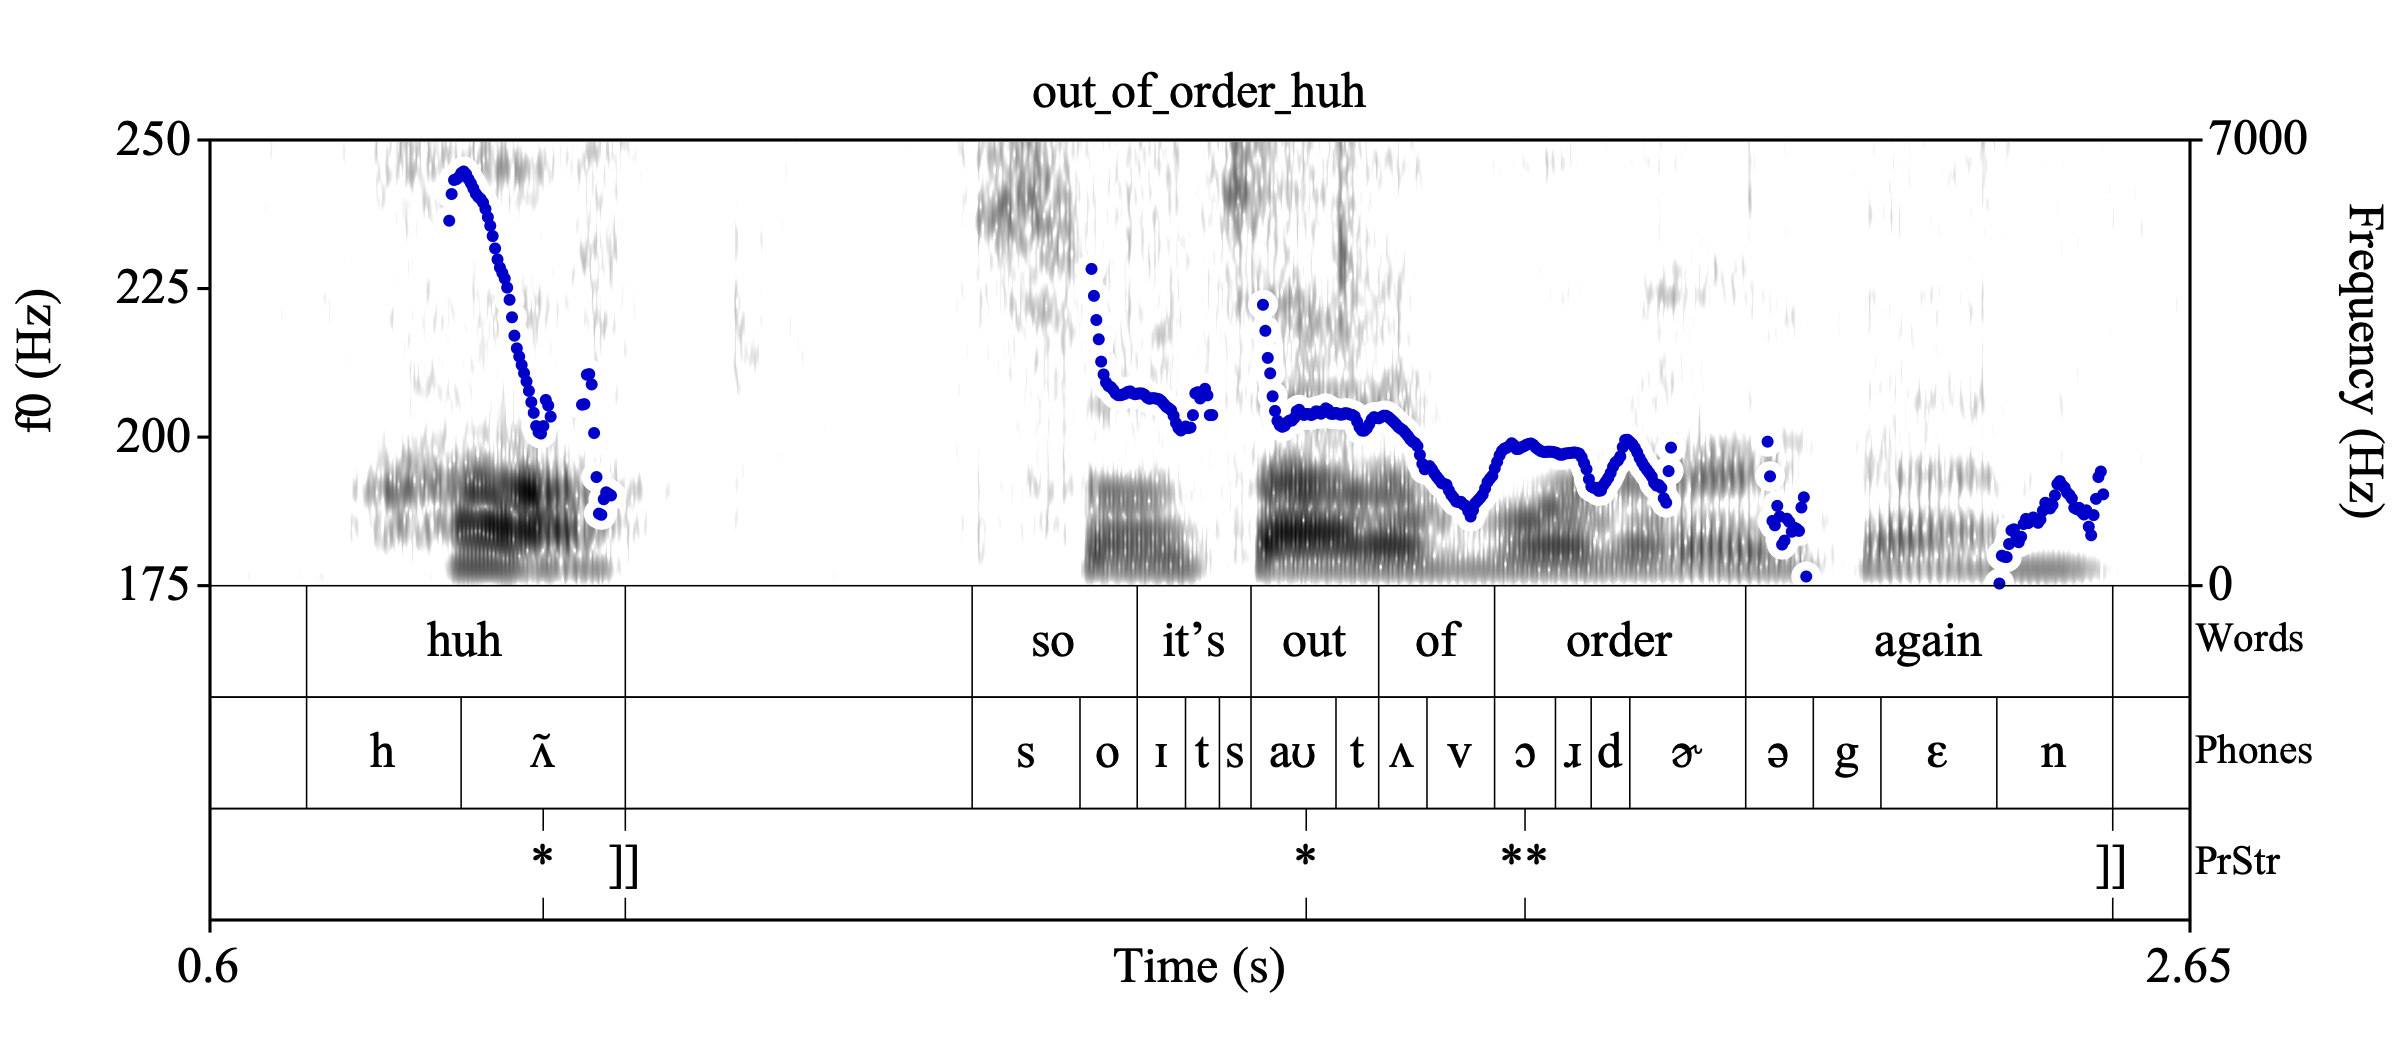
\includegraphics[width=.875\linewidth]{PrStr-out_of_order_huh-adv.png}
%
\caption[The labeller hears especially strong breaks after “\langtext{huh}” and after “\langtext{again}”.]{The labeller hears especially strong breaks after “\langtext{huh}” and after “\langtext{again}”; they also hear especially strong prominence on “\langtext{order}”.%
\label{fig:out_of_order_huh PrStr Adv}%
\index{Annotated example, PrStr tier (advanced)!out\_of\_order\_huh}
}
\end{figure}

\begin{figure}[H]
\centering
%
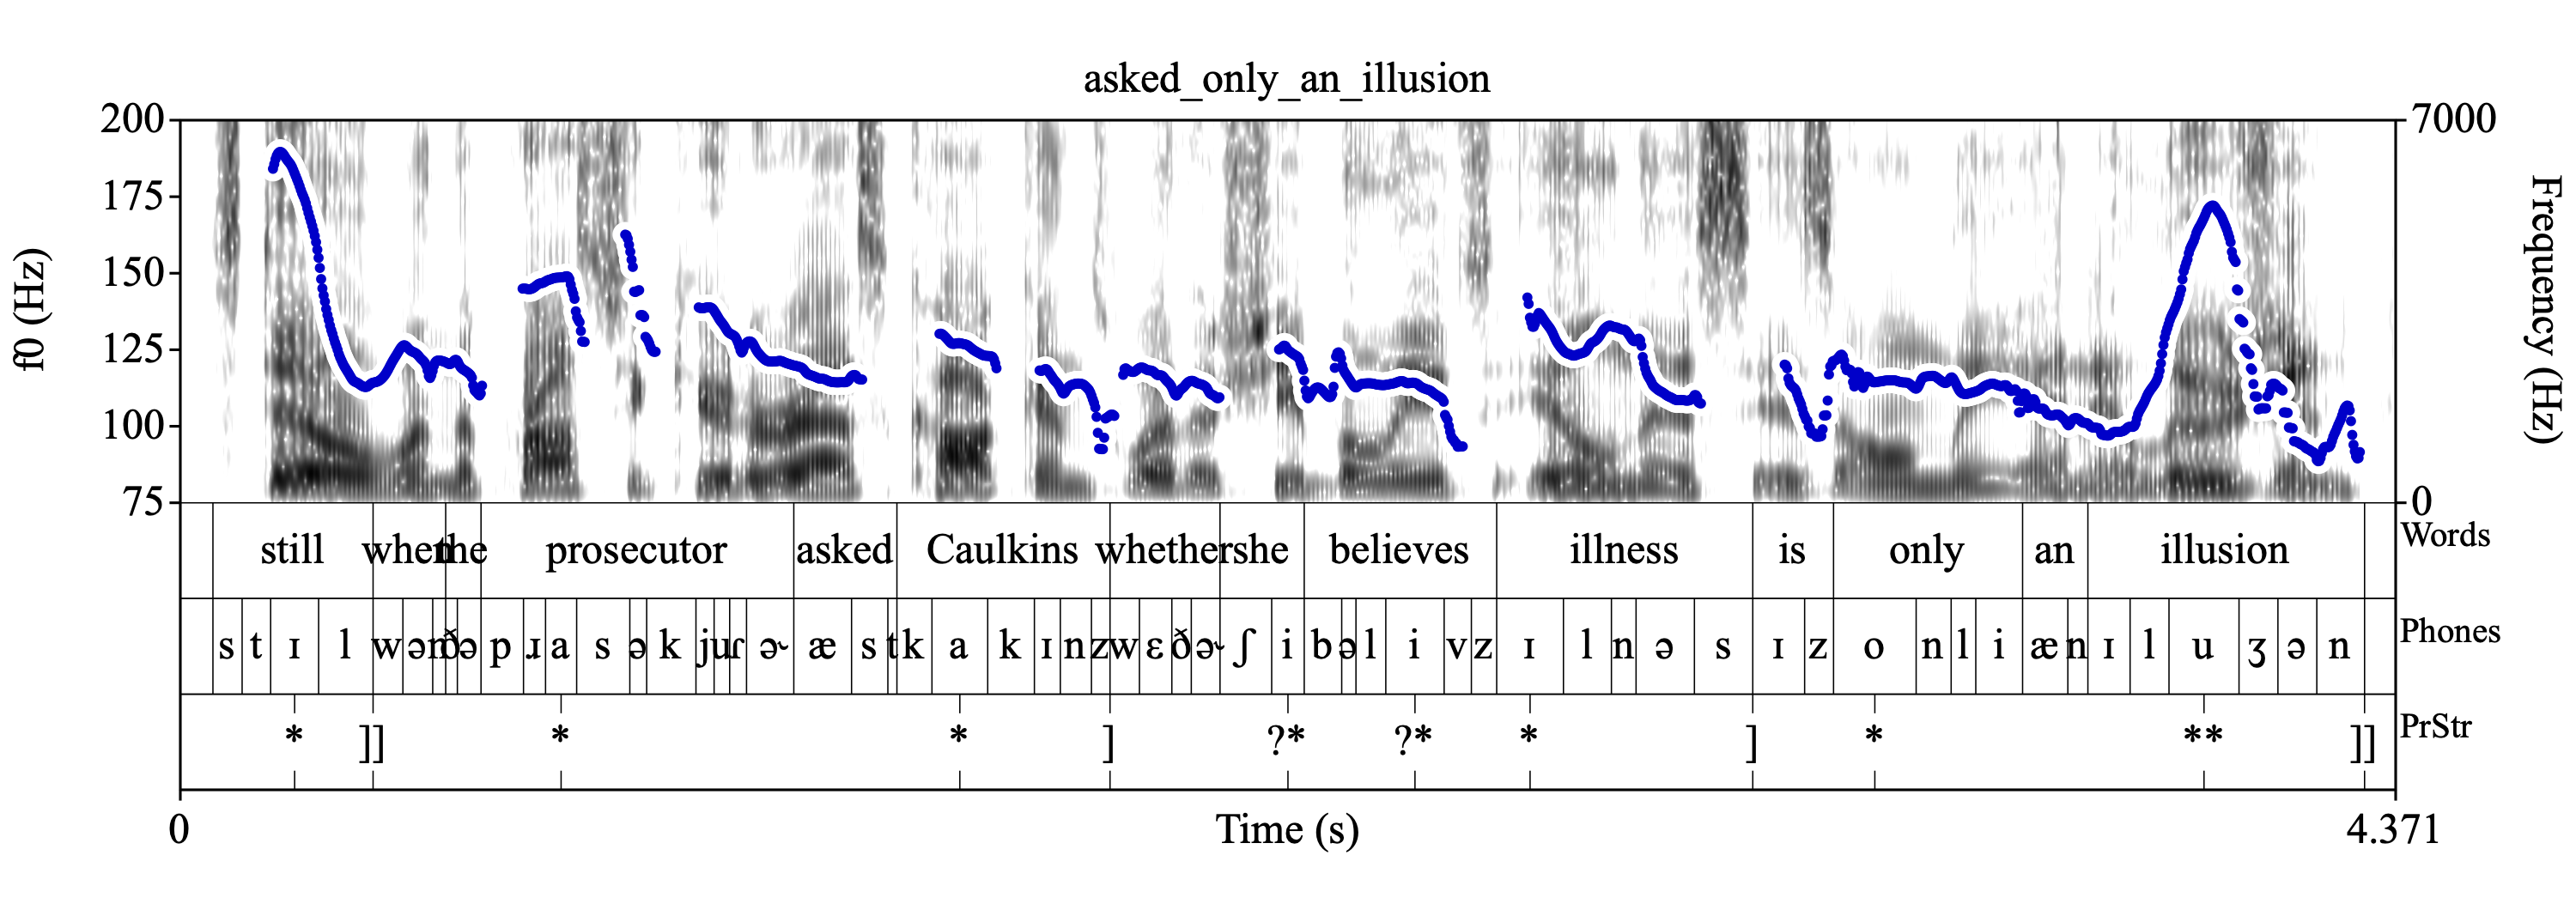
\includegraphics[width=.875\linewidth]{PrStr-asked_only_an_illusion-adv.png}
%
\caption[The labeller is at several points uncertain about prominence.]{The labeller is at several points uncertain about prominence (“\langtext{she}”, “\langtext{believes}”, “\langtext{only}”), while also hearing especially strong prominence on “\langtext{illusion}” and especially strong phrase boundaries after “\langtext{still}” and “\langtext{illusion}”.%
\label{fig:asked_only_an_illusion PrStr Adv}%
\index{Annotated example, PrStr tier (advanced)!asked\_only\_an\_illusion}
}
\end{figure}

The following example Figure \ref{fig:at_this_point-disfluencies PrStr Adv} includes instances of both labeller uncertainty about prominence (\textlabel{?*}) and a perceived a disfluency (marked with the ‘\textlabel{d}’ label). Note that some disfluencies have pauses immediately following and some do not; if it feels like the disfluency leads to new prosodic phrase boundaries, these boundaries should be annotated separately. (Likewise for disfluency-induced prominence.)

\begin{figure}[H]
\centering
%
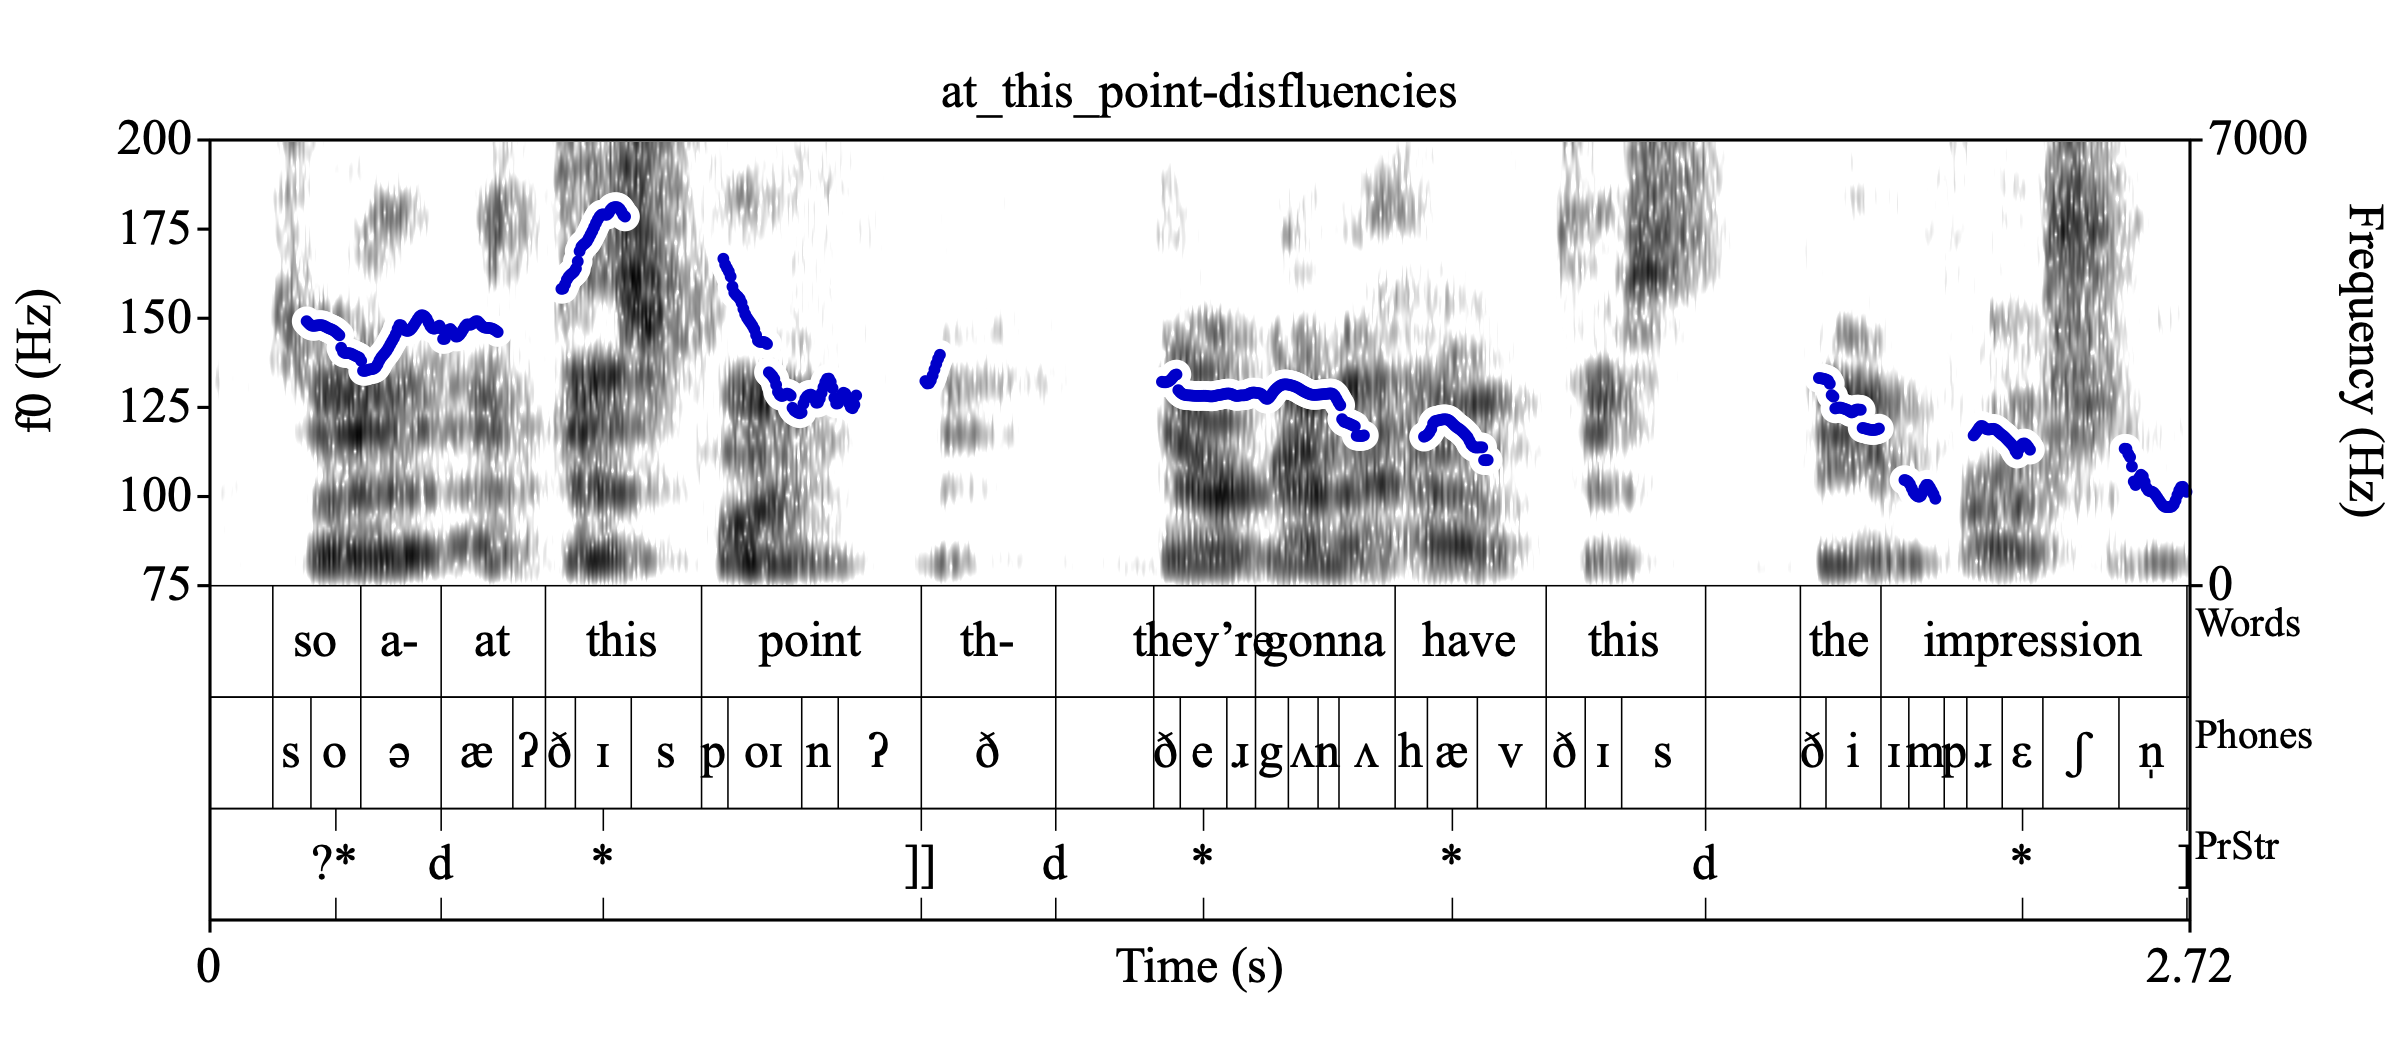
\includegraphics[width=.875\linewidth]{PrStr-at_this_point-disfluencies-adv.png}
%
\caption[The labeller hears several disfluencies.]{The labeller hears several disfluencies, where the speaker restarts\slash recasts their speech; the ‘\textlabel{d}’ labels that indicate this are at the cut-off point, before any existing disfluency-related pauses.%
\label{fig:at_this_point-disfluencies PrStr Adv}%
\index{Annotated example, PrStr tier (advanced)!at\_this\_point-disfluencies}
}
\end{figure}

\subsection{Summary of the Advanced Labels for the PrStr Tier}
This section has reviewed the Advanced labels set out for transcription in the PrStr tier. As with all Advanced labels described in this chapter, their significance and guidelines for usage are provided here, but none of the Advanced labels are required for PoLaR labellers. For example, as mentioned for the phrase-initial boundary label, \textlabel{[}, some labellers might want to use this label, while others may use it infrequently, or not at all. Similar can be said for the \textlabel{**} and disfluency-related labels.

The exhaustive list of Advanced PrStr labels are laid out in the table below, which compiles the tables found throughout this section.

\begin{longtable}{cp{.3\linewidth}p{.45\linewidth}}
	\toprule
	\textbf{Label} & \textbf{Phonological Object} & \textbf{Time-Aligned with} \tabularnewline
	\midrule
	\endhead
	\rowcolor{green}
	\textlabel{]} & Prosodic Phrase Boundary & The end of a Words interval where a prosodic phrase ends \tabularnewline
	\textlabel{?]} & Possible Prosodic Phrase Boundary & The end of a Words interval where a prosodic phrase may end (but the labeller is uncertain) \tabularnewline
	\textlabel{]]} & Large Prosodic Phrase Boundary & The end of a Words interval where a noticeably large prosodic phrase ends \tabularnewline
	\textlabel{[} & Prosodic Phrase Boundary & The beginning of a Words interval where a prosodic phrase begins \tabularnewline
	\textlabel{?[} & Possible Prosodic Phrase Boundary & The beginning of a Words interval where a prosodic phrase may begin (but the labeller is uncertain) \tabularnewline
	\textlabel{[[} & Large Prosodic Phrase Boundary & The beginning of a Words interval where a noticeably large prosodic phrase \tabularnewline
	\hline
	\rowcolor{green}
	\textlabel{*} & Prominence & The center of the Phones/Words interval that is prominent\tabularnewline
	\textlabel{?*} & Possible Prominence & The center of the Phones/Words interval that might be prominent (but the labeller is uncertain) \tabularnewline
	\textlabel{**} & Especially Strong Prominence & The center of the Phones/Words interval that is especially prominent \tabularnewline
	\hline
	\textlabel{d} & Disfluency & A point in the utterance where there is a disfluency\tabularnewline
	\textlabel{\{d} & Start of a disfluent region & A point in the utterance where a disfluent region of speech begins\tabularnewline
	\textlabel{d\}} & End of a disfluent region & A point in the utterance where a disfluent region of speech ends\tabularnewline
	\bottomrule
	\caption{The PrStr labels described in this chapter, which can be used by Advanced PoLaR labellers.}
\end{longtable}


\section{Points (Advanced)}\label{sec:points-advanced}

\subsection{Optional Advanced Labels for Relating Objects on Points Tier to Objects on Prosodic Structure Tier}\label{sec:optional-advanced-labels-for-relating-points-tier-objects-to-prosodic-structure-tier-objects}

One valuable aspect of the PoLaR system is that it allows labellers to annotate aspects of the intonational phonetics (e.g., time alignment of turning points) separately from aspects of the intonational phonology (e.g., prominences or boundaries). This independence can be achieved through using ‘\textlabel{0}’ labels on the Points tier, as we described for Basic Points labels in Chapter \ref{ch:basics}. These PoLaR Basic labels (consisting of ‘\textlabel{0}’ labels and optional comma-overrides) can be revised in a second-pass of labelling: in the first pass, PoLaR Basic Prosodic Structure and Points tiers are labelled, and in the second pass, ‘\textlabel{0}’ labels are replaced with more complex labels (described in this section) to capture relationships between the  labels on the Points tier with those on the PrStr tier. To understand these complex labels, we describe first what such labels are designed to capture, before going into the details of how to use them.

It is commonly understood that some pitch movements (like those annotated on the Points tier) are associated with (i.e., manifest cues to) particular prosodic events (like those annotated on PrStr). For example, some pitch movements are used to mark prominences, while others are used to mark boundaries. The labeller, therefore, might ask themselves if a particular turning point contributes to an intonational contours’s shape that in turn contributes to a listener’s perception of prominence or phrasing. In cases where the answer is ‘yes’, the Advanced Points labels provide the means for the labeller to capture this relationship.

Even relatively naive intonational annotators will note that pitch patterns often serve as acoustic cues to a prominence or phrase boundary. Consider the example in Figure \ref{fig:amelia_knew2 in Adv}, annotated with Basic PoLaR labels.

\begin{figure}[H]
\centering
%
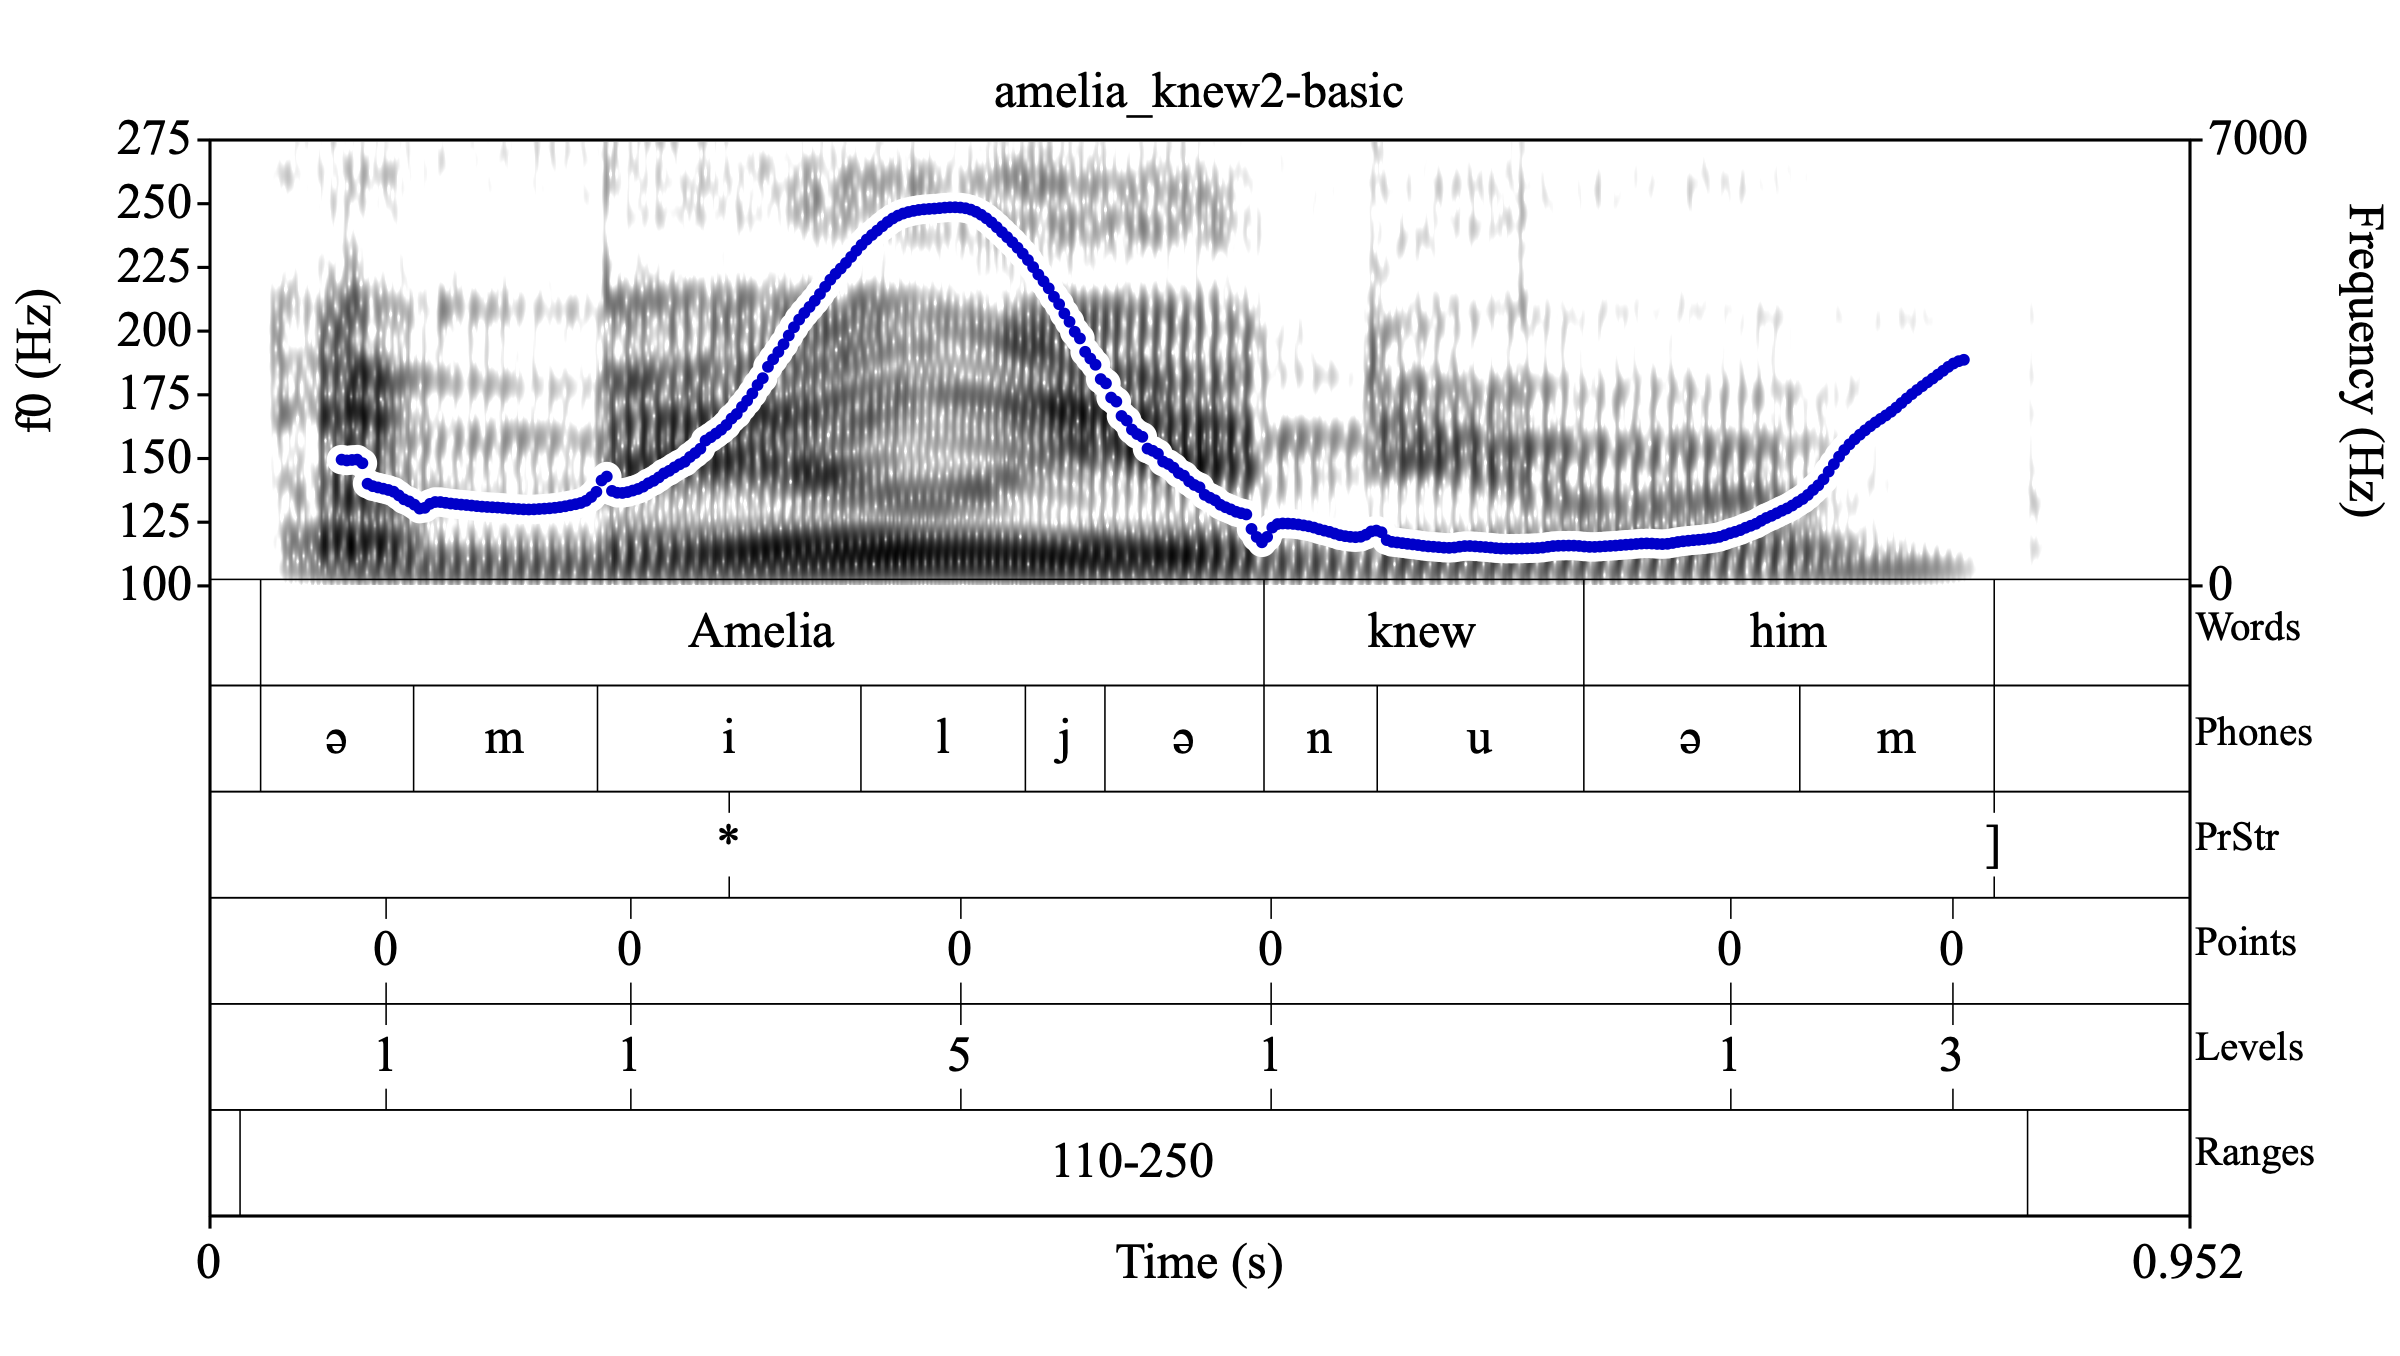
\includegraphics[width=.875\linewidth]{Points-amelia_knew2.png}
%
\caption{\texttt{amelia\_knew2}, with Basic PoLaR labels.%
\label{fig:amelia_knew2 in Adv}%
\index{Annotated example, PrStr tier (advanced)!at\_this\_point-disfluencies}
}
\end{figure}

Here the third label on the Points tier (marking the f0 peak) is cueing the prominence on “\langtext{Amelia}” labelled on the PrStr tier, while the final two labels on the Points tier (marking the phrase-final rise) cue the utterance-final phrase boundary labelled on the PrStr tier. Which, if any, of the other Points labels are related to the PrStr objects is subject to some debate, and labellers may well disagree.

Users of other annotation systems are intimately familiar with this idea; much of what many other annotation systems do is model the relationship between pitch movements and other prosodic objects. Systems that do this include those that make an important distinction between pitch movements of various types; e.g., IPO, ToBI, IViE, or RaP. Because of this, such labellers have strong intuitions whether a particular f0 turning point “belongs to” a prominence (i.e., manifests a cue for a pitch accent) or a phrase boundary (i.e., manifests a cue for an edge tone). PoLaR labellers who are familiar with those models are encouraged to use their background in these other models to inform how they relate Points and PrStr objects with Advanced Points labels. (Note this means users with different theoretical priors may well label the same Basic Points labels of a single utterance with different Advanced Points labels - we take this to be a feature, not a bug.)

Below we provide a more comprehensive description of the Advanced PoLaR labels that can replace pitch turning points that are originally marked with a ‘\textlabel{0}’ on the Points tier, to indicate that a given turning point is perceived to be prominence-marking or edge-marking (or both). A PoLaR Advanced Points label consists of a minimum of two components: (i) the \textit{\uline{type}} of phonological object the turning point is associated with, and (ii) a \textit{\uline{pointer}} to the relevant Prosodic Structure tier label’s time coordinate. We find that there are three different scenarios that arise when deciding whether a turning point is associated with a prosodic event labelled on the PrStr tier, and if so, with which one:

\begin{enumerate} \def\labelenumi{\arabic{enumi}.}
\item No PrStr labelled event is associated with the f0 turning point, or it’s not clear that one is. In this case, use ‘\textlabel{0}’ as the complete label. (This is a ‘neutral’ label, indicating that the labeller is not committing to any particular analysis, but has determined that a significant turning point needs to be marked at that location.)
\item A particular \textit{\uline{type}} of PrStr labelled event (either ‘\textlabel{*}’ or ‘\textlabel{]}’; marked below as ‘\textlabel{\_}’) is associated with the f0 turning point, which is time-aligned in various ways, indicated by one of three \textit{\uline{pointer}}s:

 \begin{enumerate} \def\labelenumii{\alph{enumii}.}
\item PrStr label follows Points label (‘\textlabel{\_>}’)
\item PrStr label precedes Points label (‘\textlabel{\_<}’)
\item {[\textit{uncommon}]} PrStr label is precisely co-timed with Points label (‘\textlabel{\_@}’) \end{enumerate}
\item Occasionally, multiple PrStr labelled events are associated with a single f0 turning point. That is, the turning point is either (i) ambiguous between being associated with the preceding PrStr labelled event and being associated with the following event, or (ii) the labeller believes that the point relates to both of those events. In these cases a complex label is used, with two labels separated by a \textlabel{/} (‘\textlabel{\_</\_>}’). \end{enumerate}

There are two observations to be made about these labels right away. First, any non-‘\textlabel{0}’ label on the Points tier indicates the labeller has an intuition about the appropriate analysis. Thus, in the absence of such an intuition, the advanced labeller should leave the ‘\textlabel{0}’ label in place.

Second, the pointers themselves (‘\textlabel{>}’, ‘\textlabel{<}’, ‘\textlabel{@}’) carry no significance beyond indicating a relationship of how a PrStr label and a Points label happen to be time-aligned. That is, because the timing of a PrStr label is at the discretion of the labeller, its precise location in time is not meaningful.  Thus, a label ‘\textlabel{*>}’ in the Points tier simply means that “this turning point manifests a cue to the prominence labelled as a ‘\textlabel{*}’ on the Prosodic Structure tier, which is time-aligned later than (to the right of) this Points tier label.” A minimally different label, ‘\textlabel{*<}’, says that the relevant PrStr ‘\textlabel{*}’ label is time-aligned earlier than the Points tier label. To repeat, in the interest of clarity: these two labels are not in and of themselves informatively different, in part because the particular timing of the PrStr label is not informative.\footnote{In other words, the difference between, e.g., ‘\textlabel{*>}’ and ‘\textlabel{*<}’ is not a meaningful one; it may simply be a reflection of how the ‘\textlabel{*}’ label happens to be timed – which is at the whim of the labeller. (Recall that the ‘\textlabel{*}’ label on the PrStr tier need only be time-aligned within the stressed vowel.) This may be somewhat surprising for labellers familiar with other annotation systems, where labels that use different symbols in a label are meant to signify meaningful\slash phonological distinctions (e.g., \textlabel{L+H*} vs. \textlabel{L*+H} in ToBI or \textlabel{H*L} vs. \textlabel{!H*L} in IViE).}

The options and the order of the notation is summarized below. (A more complete grammar for Points tier labels is provided in section \ref{sec:summary-of-the-points-tier}.)

\begin{figure}[H]
\centering
%
  \begin{tikzpicture}[node distance=4em, anchor=west, align=flush center, FLOW/.style={->, very thick}, LABEL/.style={draw, fill=yellow!80, inner sep=.75em}, scale = .775, transform shape]
    \node[draw, text width=5.5em] (node2) {Assert a relationship to a PrStr object?};
    \node[LABEL, below right=1em and 6em of node2.east] (node3no) {\textlabel{0}};
    \node[LABEL, above right=1em and 6em of node2.east] (node3yes) {\textlabel{*}\\\textlabel{]}\\\textlabel{[}};
    \node[draw, text width=8em, right=3em of node3yes] (node4) {Where is the PrStr Tier object that corresponds to the Points Tier object?};
    \node[LABEL, right=3em of node4.east] (node5) {\textlabel{>}\\\textlabel{<}\\\textlabel{@}};
    \node[draw, text width=8em, below=1.5em of node5, anchor=north] (node6) {Could this Points Tier object also correspond to another PrStr object?};
    \node[right=3em of node6] (node7yes) {};
    \node[LABEL, above=of node7yes.center] (node7) {\textlabel{/}};
    \node[above=5em of node7] (node7-loopback1) {};
    \node[above=2em of node3yes] (node7-loopback2) {};
%%%%%%%%%%%%%%%
%%%%%%%%%%%%%%%
    \draw [black,FLOW] (node2.east) -- node[pos=0.5, above, sloped]{Yes} (node3yes.west);
    \draw [black,FLOW] (node2.east) -- node[pos=0.5, above, sloped]{No} (node3no.west);
    \draw [black,FLOW] (node3yes.east) -- (node4.west);
    \draw [black,FLOW] (node4.east) -- (node5.west);
    \draw [black,FLOW] (node5.south) -- (node6.north);
    \draw [black,FLOW] (node6.east) -- node[pos=0.5, above, sloped]{Yes} (node7yes.center) -- (node7.south);
    \draw [black,FLOW] (node7.north) --  (node7-loopback1.center) -- (node7-loopback2.center) -- (node3yes);

  \end{tikzpicture}
%
\caption{A grammar of the core Advanced Points tier labels.%
\label{fig:Points FSG basic}%
%\index{}
}
\end{figure}

In summary, these Advanced Points tier labels are either (1) the simple ‘\textlabel{0}’ label, (2) a complex label with two components in the order \textit{<{type}>{}} \textit{<{pointer}>}, or (3) a label made up of two complex labels separated by a \textlabel{/}.

\begin{longtable}{cp{.8\linewidth}}
\toprule
\textbf{Type Label} & \textbf{Relationship with a Prosodic Structure Tier Object}\tabularnewline\hdashline
\textlabel{0} & The default label is still the most appropriate choice if the annotator chooses not to affiliate a turning point with a Prosodic Structure label. (No pointer is used in conjunction with a ‘\textlabel{0}’ label.) \tabularnewline\hdashline
\textlabel{*} & An f0 turning point for a \textlabel{*} (\textit{of any type; e.g., also \textlabel{**} or \textlabel{?*}}) in the Prosodic Structure tier \tabularnewline\hdashline
\textlabel{]} & An f0 turning point for a \textlabel{]} (\textit{also \textlabel{?]} or \textlabel{]]}}) in the Prosodic Structure tier \tabularnewline\hdashline
\textlabel{[} & An f0 turning point for a \textlabel{[} (\textit{also \textlabel{?[} or \textlabel{[[}}) in the Prosodic Structure tier \tabularnewline
\midrule
\textbf{Pointer Label} & \textbf{Timing of the relevant Prosodic Structure Tier Object}\tabularnewline\hdashline
\textlabel{>{}} & This f0 turning point is related to a Prosodic Structure tier object that follows it \tabularnewline\hdashline
\textlabel{<{}} & This f0 turning point is related to a Prosodic Structure tier object that precedes it \tabularnewline\hdashline
\textlabel{@} & This f0 turning point is related to a Prosodic Structure tier object that is precisely aligned with it \tabularnewline
\midrule
\textbf{Special Label} & \textbf{Noted ambiguity} \tabularnewline\hdashline
\textlabel{/} & This f0 turning point’s affiliation is ambiguous; it may be related to the Prosodic Structure event before the turning point, or to the Prosodic Structure event that follows it. \tabularnewline
\bottomrule
\caption[Advanced Points labels]{Advanced Points labels: The possible types of phonological object that a turning point is related to, and the pointers to the location of the Prosodic Structure Tier object in time. By default, a labeller does not offer a phonological analysis, using the label that is highlighted.}
\end{longtable}

\subsection{Some Introductory Examples of Advanced Points Labels}\label{sec:some-first-examples-of-advanced-points-labels}

A simple Advanced Points label is shown in Figure \ref{fig:me Points Adv}. This is a more complete label of this file, which is shown earlier with its Basic Point labels as Figure \ref{fig:me Points basic} in Chapter \ref{ch:basics}). The ‘\textlabel{*>}’ on the Points tier is pointing rightward to the ‘\textlabel{*}’ label on the PrStr tier that follows it, indicating the labeller’s judgment that this turning point helps to cue the prominence marked by the ‘\textlabel{*}’.\footnote{Here the ‘\textlabel{*}’ label on the Prosodic Structure tier is time-aligned to the precise middle of the stressed vowel interval (as determined by a forced-aligner). This illustrates the general principle that no Prosodic Structure tier object is aligned in any particular way with respect to f0 movements.}

\begin{figure}[H]
\centering
%
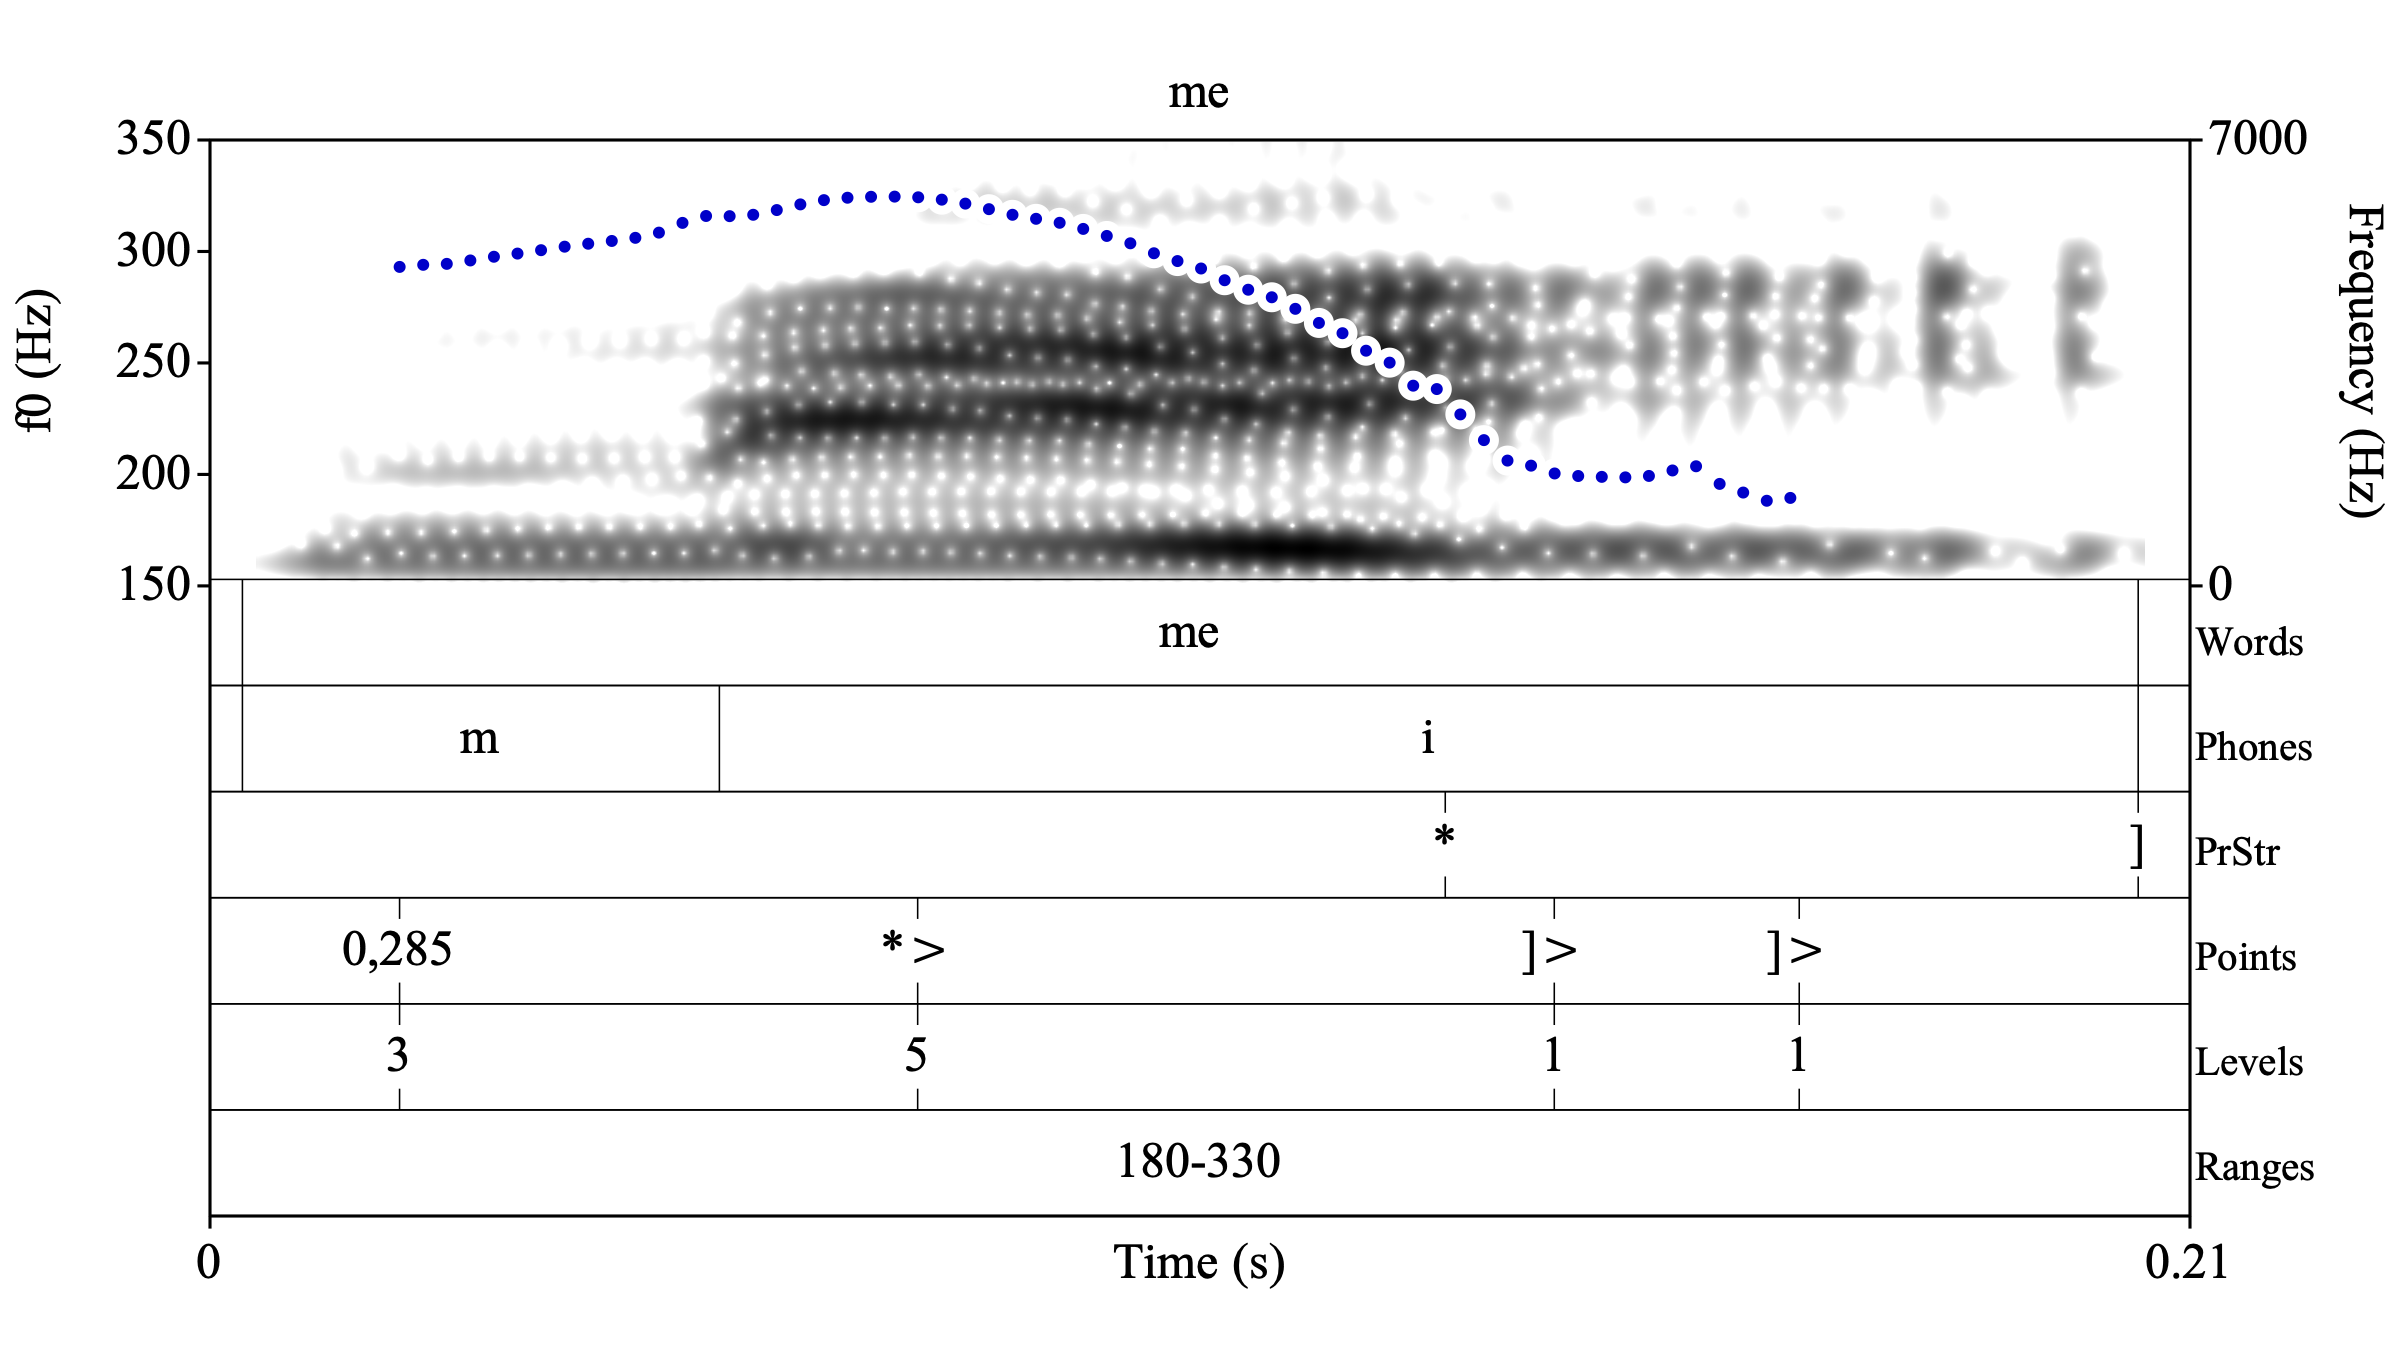
\includegraphics[width=.875\linewidth]{Points-me-adv.png}
%
\caption{\texttt{me}, with Advanced PoLaR labels.%
\label{fig:me Points Adv}%
\index{Annotated example, Points tier (advanced)!me}
}
\end{figure}

This example also shows the usage of the ‘\textlabel{]>}’ label. This indicates that the f0 movement labelled by the third and fourth points tier labels (formerly ‘\textlabel{0}’s) are related to the following phrase boundary, labelled with a \textlabel{]} on the Prosodic Structure tier. Note that there are \textit{\uline{two}} of these labels for this recording: one to mark the beginning of the low flat f0 that signals the end of the phrase (cf. ToBI phrase accents), and one to mark the end of that plateau. Also note that the final ‘\textlabel{]>}’ label is not timed to be at (or even near to) the PrStr ‘\textlabel{]}’, but rather to label the end of the reliable f0 track.

A second example, shown below, was also presented as Figure \ref{fig:really_would_not_annoy Points basic} during the discussion of Basic ‘\textlabel{0}’ Point tier labels in Chapter \ref{ch:basics}.

\begin{figure}[H]
\centering
%
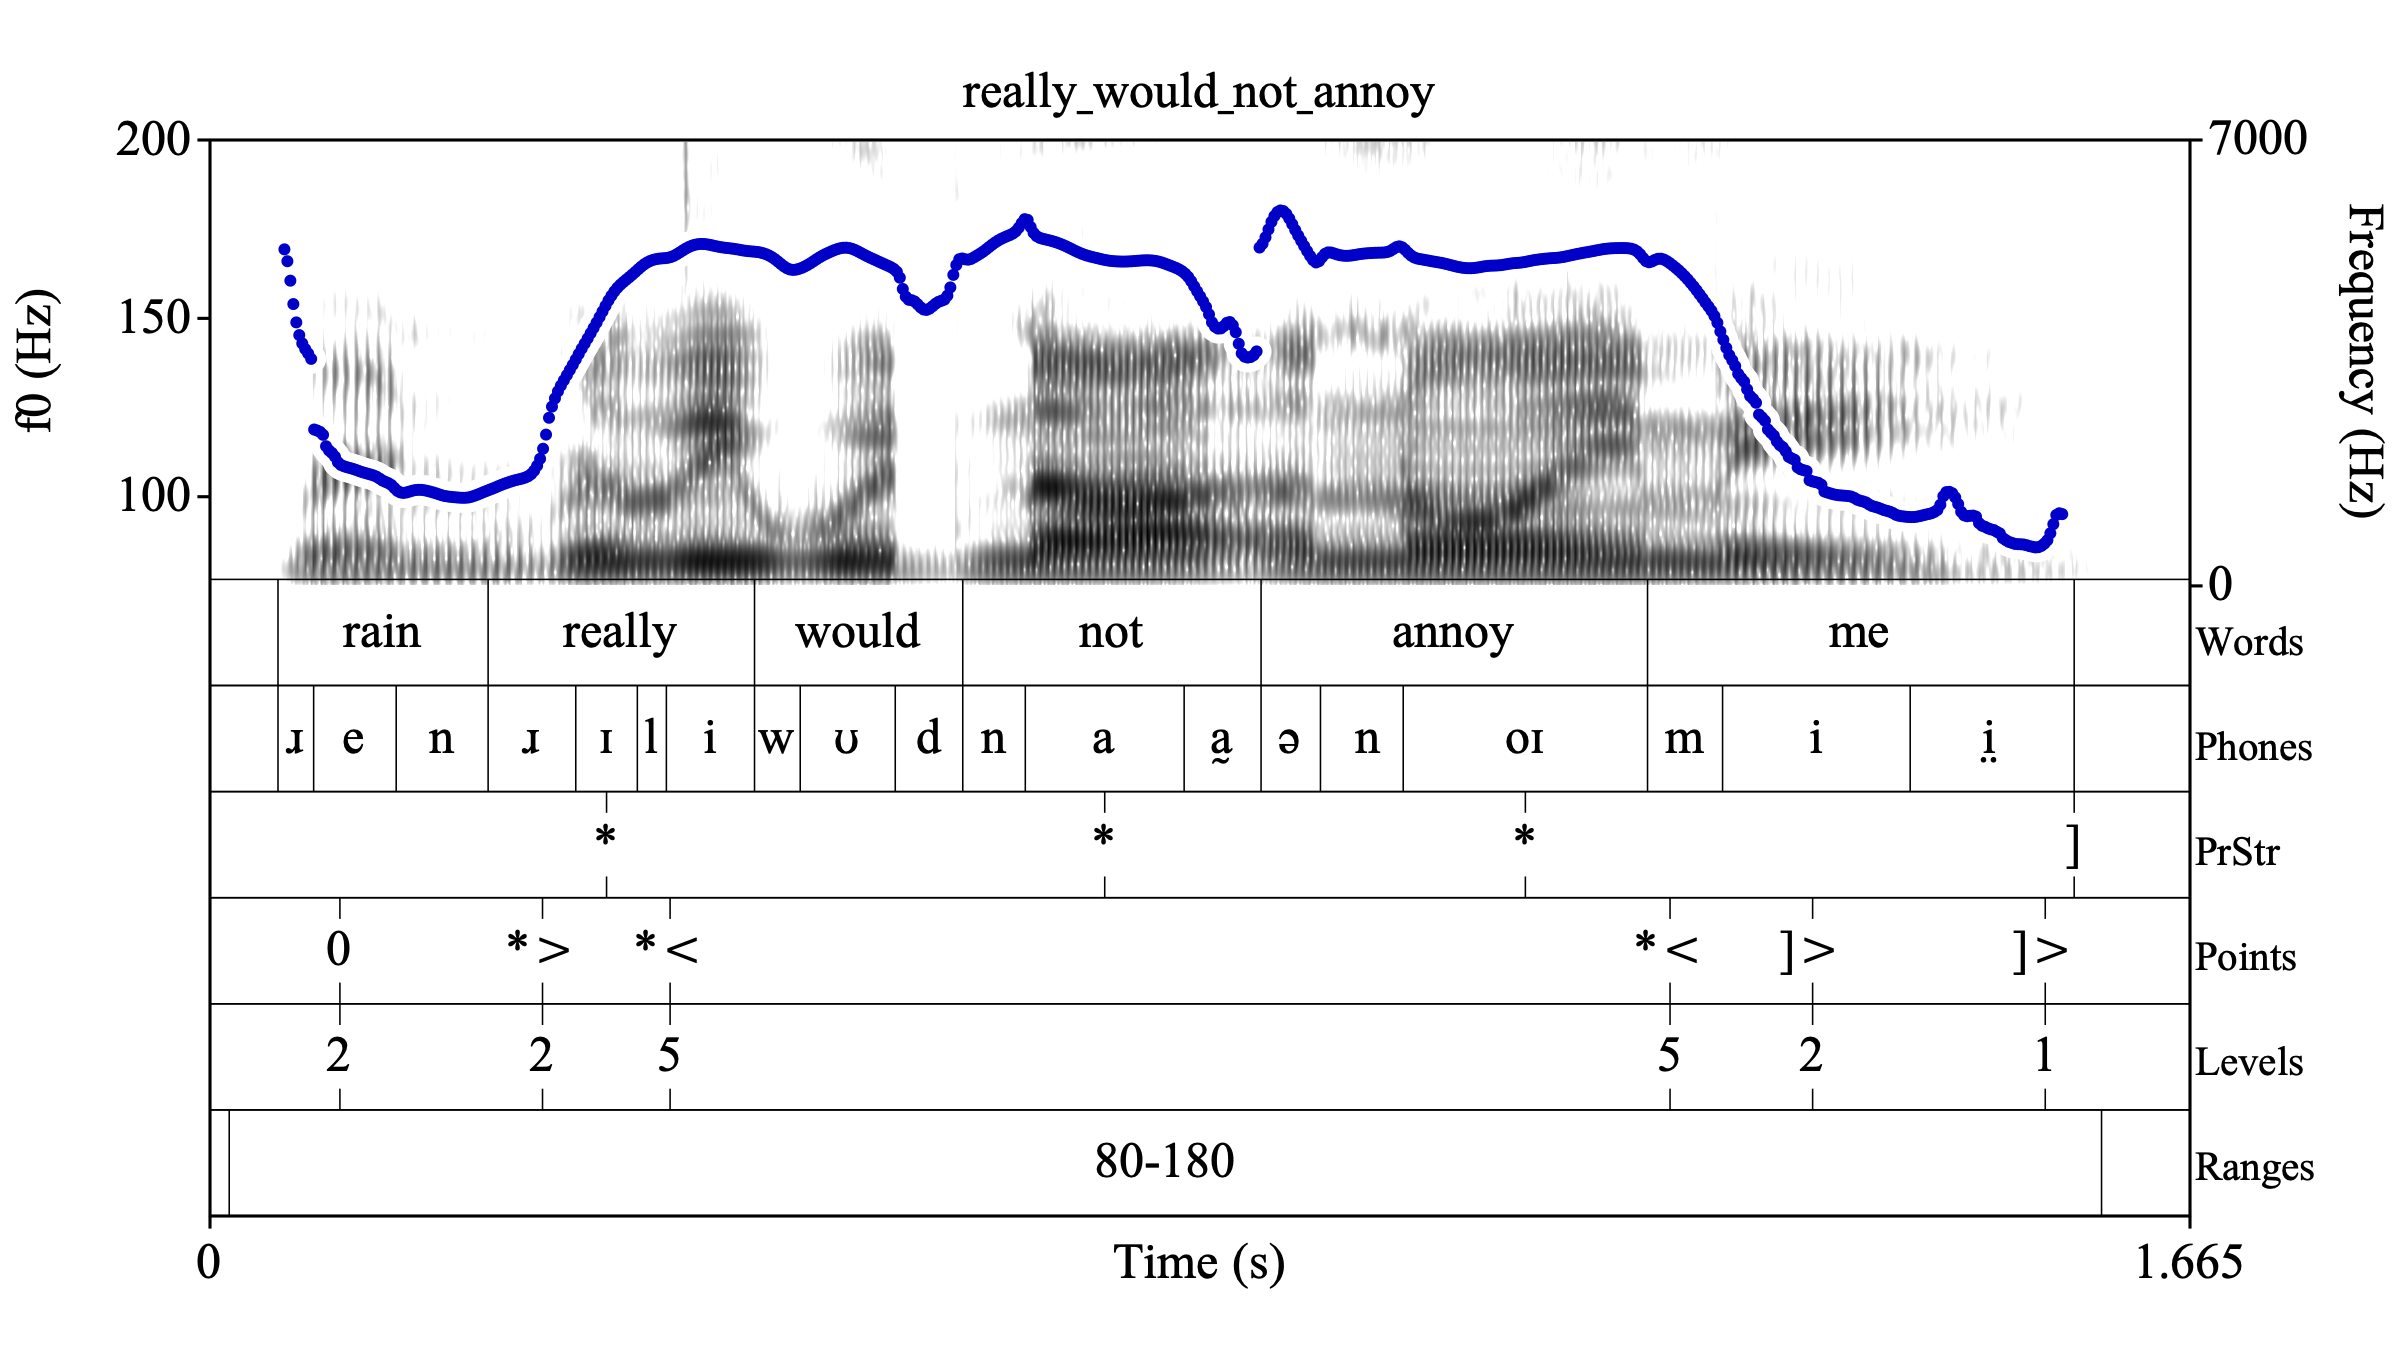
\includegraphics[width=.875\linewidth]{Points-really_would_not_annoy-adv.png}
%
\caption{\texttt{really\_would\_not\_annoy}, with Advanced PoLaR labels.%
\label{fig:really_would_not_annoy Points Adv}%
\index{Annotated example, Points tier (advanced)!really\_would\_not\_annoy}
}
\end{figure}

Again, note that the Points tier labels ignore unreliable pitch tracks (such as the very high pitch tracking at the beginning of “\langtext{rain}”, the dip in the [d] of “\langtext{would}”, the perturbations between “\langtext{not}” and “\langtext{annoy}”, etc.). For further discussion of such phenomena, the reader is referred to Chapter \ref{ch:basics} (specifically section \ref{sec:intonational-contours-and-software-based-pitch-tracks}), for its discussion of pitch track disruptions (a.k.a. “microprosody”).

The first Point tier label, therefore, occurs where the initial f0 becomes reliable. Because that turning point is not perceived to contribute to any of the Prosodic Structure (PrStr) events, the ‘\textlabel{0}’ label remains. The second and third Point tier labels are determined to be related to the prominence on the word “\langtext{really}” and so the default ‘\textlabel{0}’ label is replaced with a \textlabel{*} to indicate its relationship to a prominence (rather than a phrase break) and the ‘\textlabel{>}’ and ‘\textlabel{<}’ pointers further indicate which prominence: the one labelled in the middle of the vowel in the first syllable of “\langtext{really}” in the Prosodic Structure Tier above.

Notably, “\langtext{not}”, though prominent, is not marked by any label on the Points tier; it occurs in the middle of a high plateau. To emphasize: not every prominence or phrase boundary in PrStr necessarily corresponds to a Points tier label. The fourth Points tier label is determined to be related to the prominence on “\langtext{annoy}”, marked at an earlier time point in the PrStr tier. Finally, the last two Points tier labels are associated with the final low phrase break to their right.

A broader point illustrated by this example is that there is no minimum or maximum number of Points tier objects that are related to a given PrStr tier object. Each of the three \textlabel{*} labels in this example is related to a different number of Points labels (in temporal order, the PrStr \textlabel{*}s are affiliated with two, zero, and one Points labels, respectively).

\subsection{Ambiguous Association with a PrStr Object}\label{sec:ambiguous-association-with-a-prstr-object}

There are situations where a turning point in the f0 contour might reasonably be analyzed as associated with multiple prosodic elements. This could be a situation of indeterminacy: i.e., the labeller does not have enough information to decide one way or another. Alternatively, a labeller might have reason to believe that there are \uline{two} turning points, at an abstract level of the speaker’s intentions, but the acoustic signal is such that only one turning point is identifiable.

As an example, if a prominent syllable is phrase-final, a turning point could be associated with the \textlabel{*} or the \textlabel{]} on the PrStr tier, both of which are labelled on the same syllable. This is illustrated by the word \langtext{beans} in Figure \ref{fig:vegetable_list Points Adv} below.

\begin{figure}[H]
\centering
%
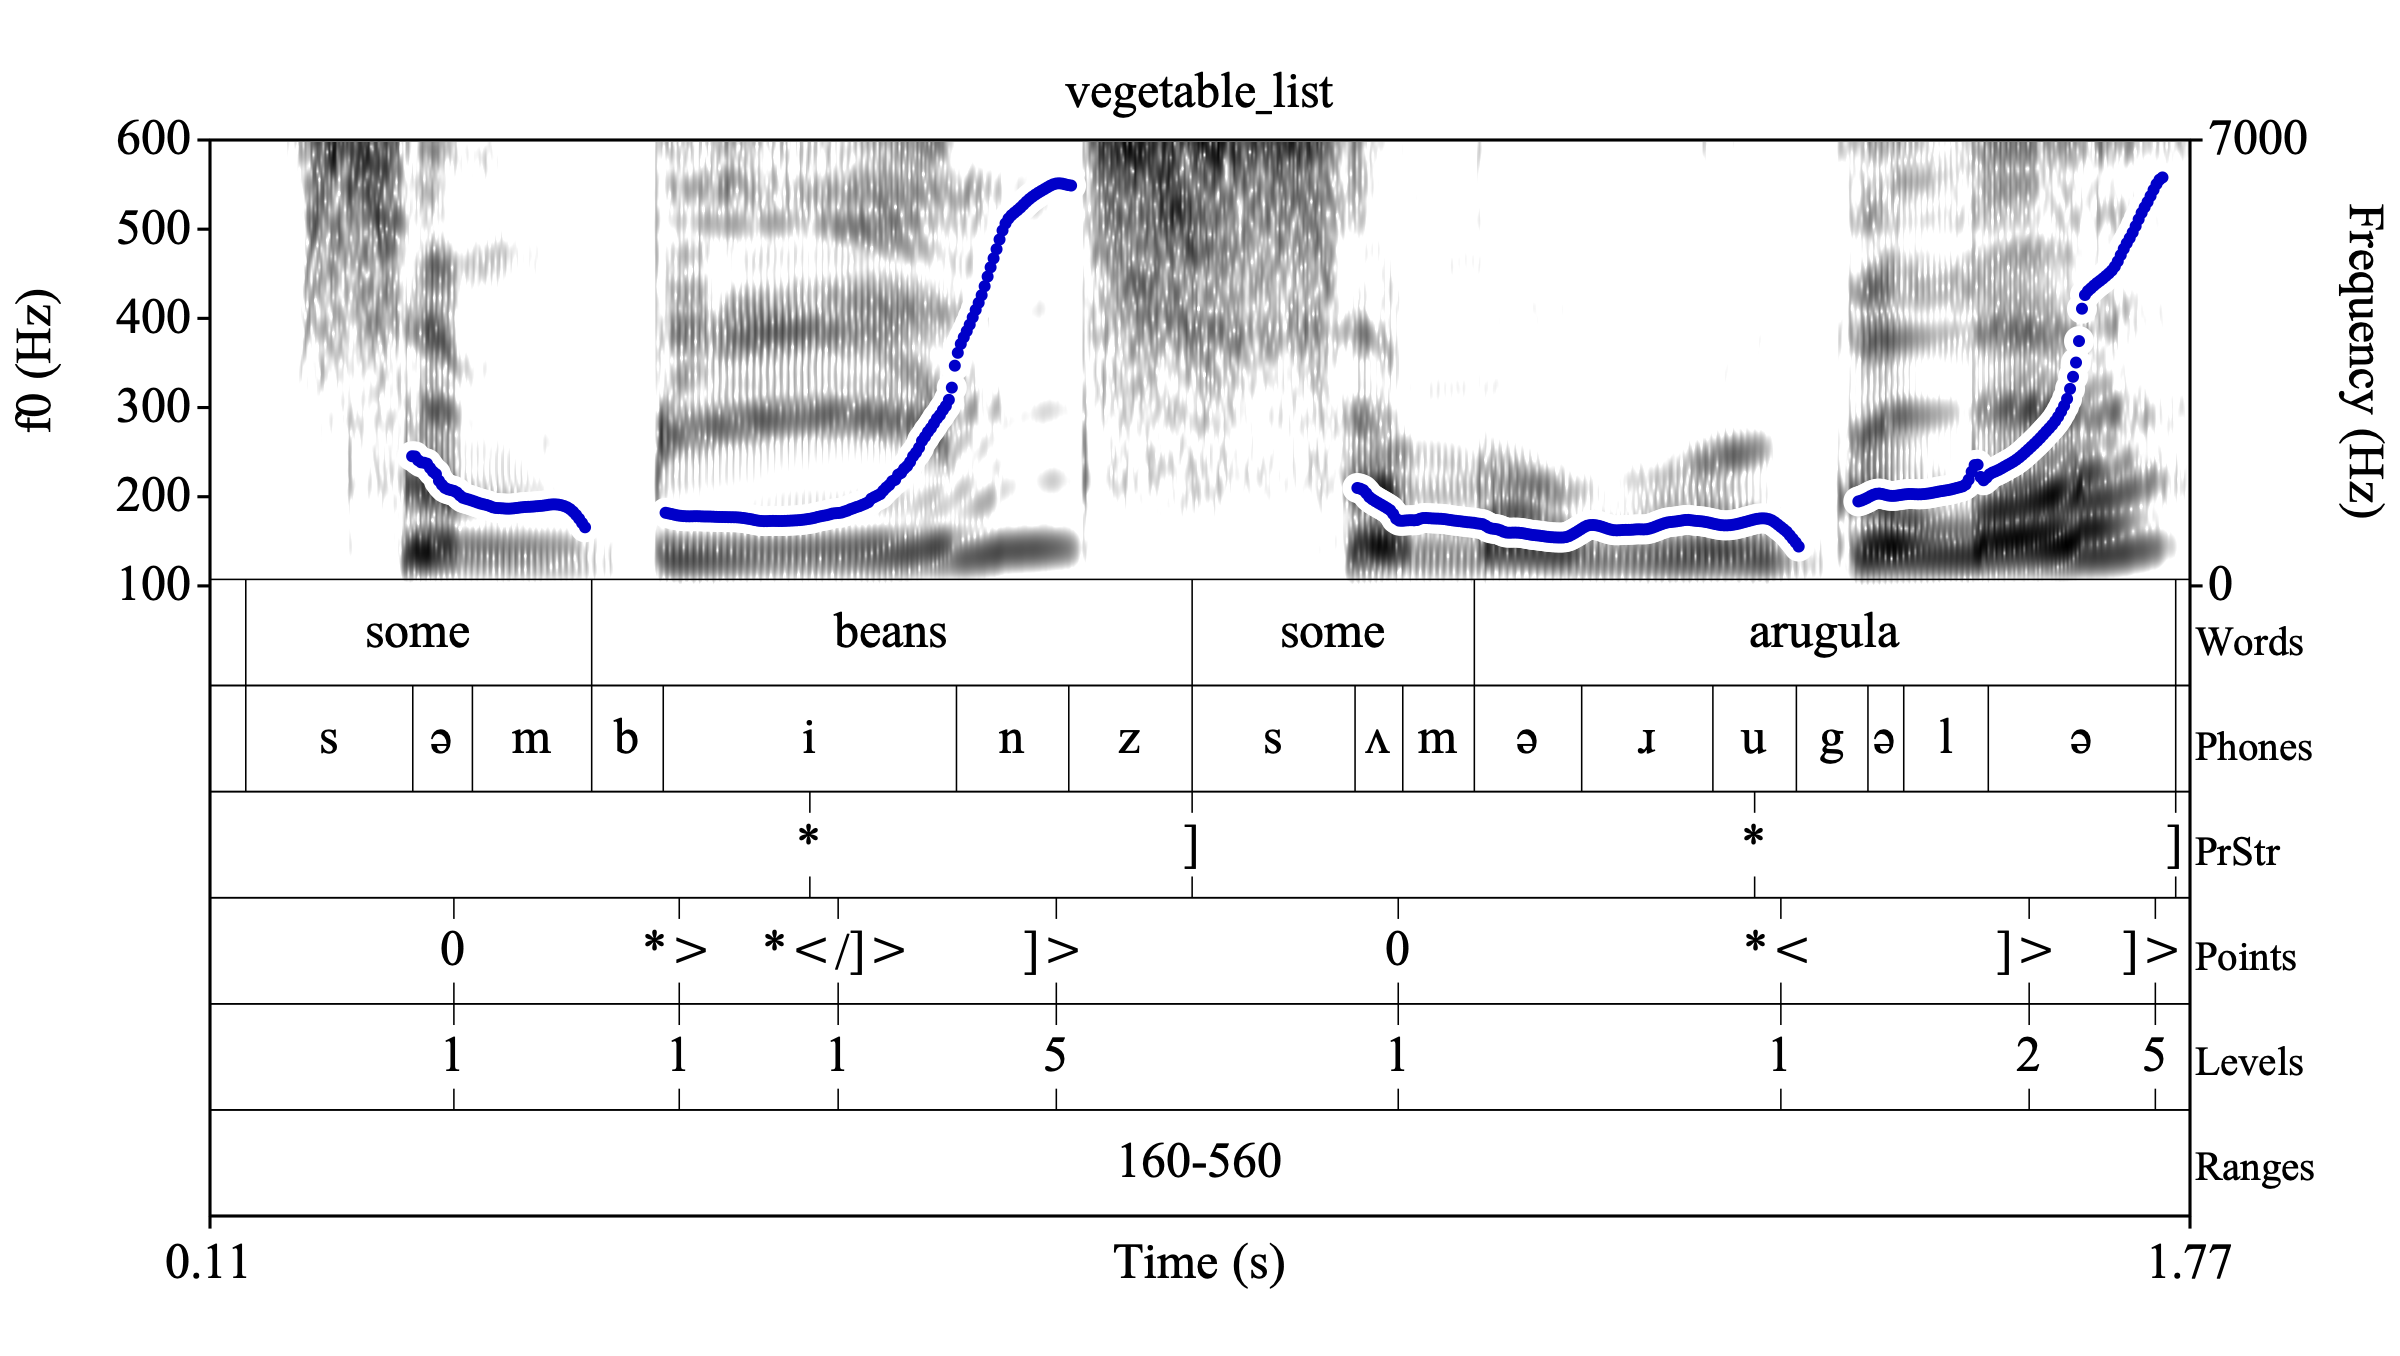
\includegraphics[width=.875\linewidth]{Points-vegetable_list-adv.png}
%
\caption[The [i] vowel in \langtext{beans} is prominent and is also phrase-final.]{The [i] vowel in \langtext{beans} is prominent and is also phrase-final. The low f0 could be associated with the \textlabel{*} (i.e., a low pitch accent), or it could also be associated with the \textlabel{]} (i.e., as the beginning of a final rise edge tone).%
\label{fig:vegetable_list Points Adv}%
\index{Annotated example, Points tier (advanced)!vegetable\_list}
}
\end{figure}

Rather than require the labeller to arbitrarily assign the turning point label leftward or rightward, the \textlabel{/} can be used between two labels, allowing the labeller to indicate that they believe both PrStr associations are plausible. This is the case in Figure \ref{fig:vegetable_list Points Adv}, where ‘\textlabel{*</]>}’ means the turning point could be associated with the ‘\textlabel{*}’ on the PrStr tier that precedes the Point or with the ‘\textlabel{]}’ on the PrStr tier that follows it. Listeners hear “the same” intonational contour being relevant for both \langtext{beans} and \langtext{arugula}; note the similarities between the two, in particular with respect to their Points labels. While there are two Points labels annotated in \langtext{beans} and three in \langtext{arugula}, the analysis in them is the same: there is a low point related to the prominence ‘\textlabel{(*<)}’, another low(ish) points related to the boundary (‘\textlabel{]>}’), and a high point related to the boundary ‘\textlabel{(]>)}’. It just happens that in \langtext{beans}, two of these relationships are annotated at the same point in time (‘\textlabel{*</]>}’). The additional syllables in \langtext{arugula} (particularly between the prominent [ɹu] and the phrase-final boundary) provide enough time to see more clearly the motivation for each of the prominence and boundary being associated with a “low” point in the intonation.

Similar to this usage of ‘\textlabel{*</]>}’, the \textlabel{/} can be used to create compound labels like ‘\textlabel{*</*>}’, ‘\textlabel{*>/]>}’, ‘\textlabel{]</*>}’, etc. Additional examples with compound labels like this will be found in the following sections.

\subsection{Points associated with phrase-initial boundaries}\label{sec:points-associated-with-phrase-initial-boundaries}
While AM annotation conventions typically annotate only the boundary at the end of a phrase, PoLaR allows the flexibility of optionally marking the beginning of a phrase. In such cases, there may be f0 turning points that the labeller would like to attribute to an initial boundary. A widely-known circumstance in which this may occur is for a high initial f0 in a phrase that is not clearly associated with a prominence. (I.e. those rare cases that are labelled \textlabel{\%H} in ToBI.) With PoLaR, the labeller may choose to assign any or all phrase-initial turning points to a \textlabel{[} boundary marker.

The example below shows a case where an initial high f0 has been attributed to an initial High boundary tone (\textlabel{\%H}) in ToBI training materials. In PoLaR, such a case could be labelled with a \textlabel{[} in the PrStr tier, and an early high f0 point in the Points tier with a \textlabel{[<} label:

\begin{figure}[H]
\centering
%
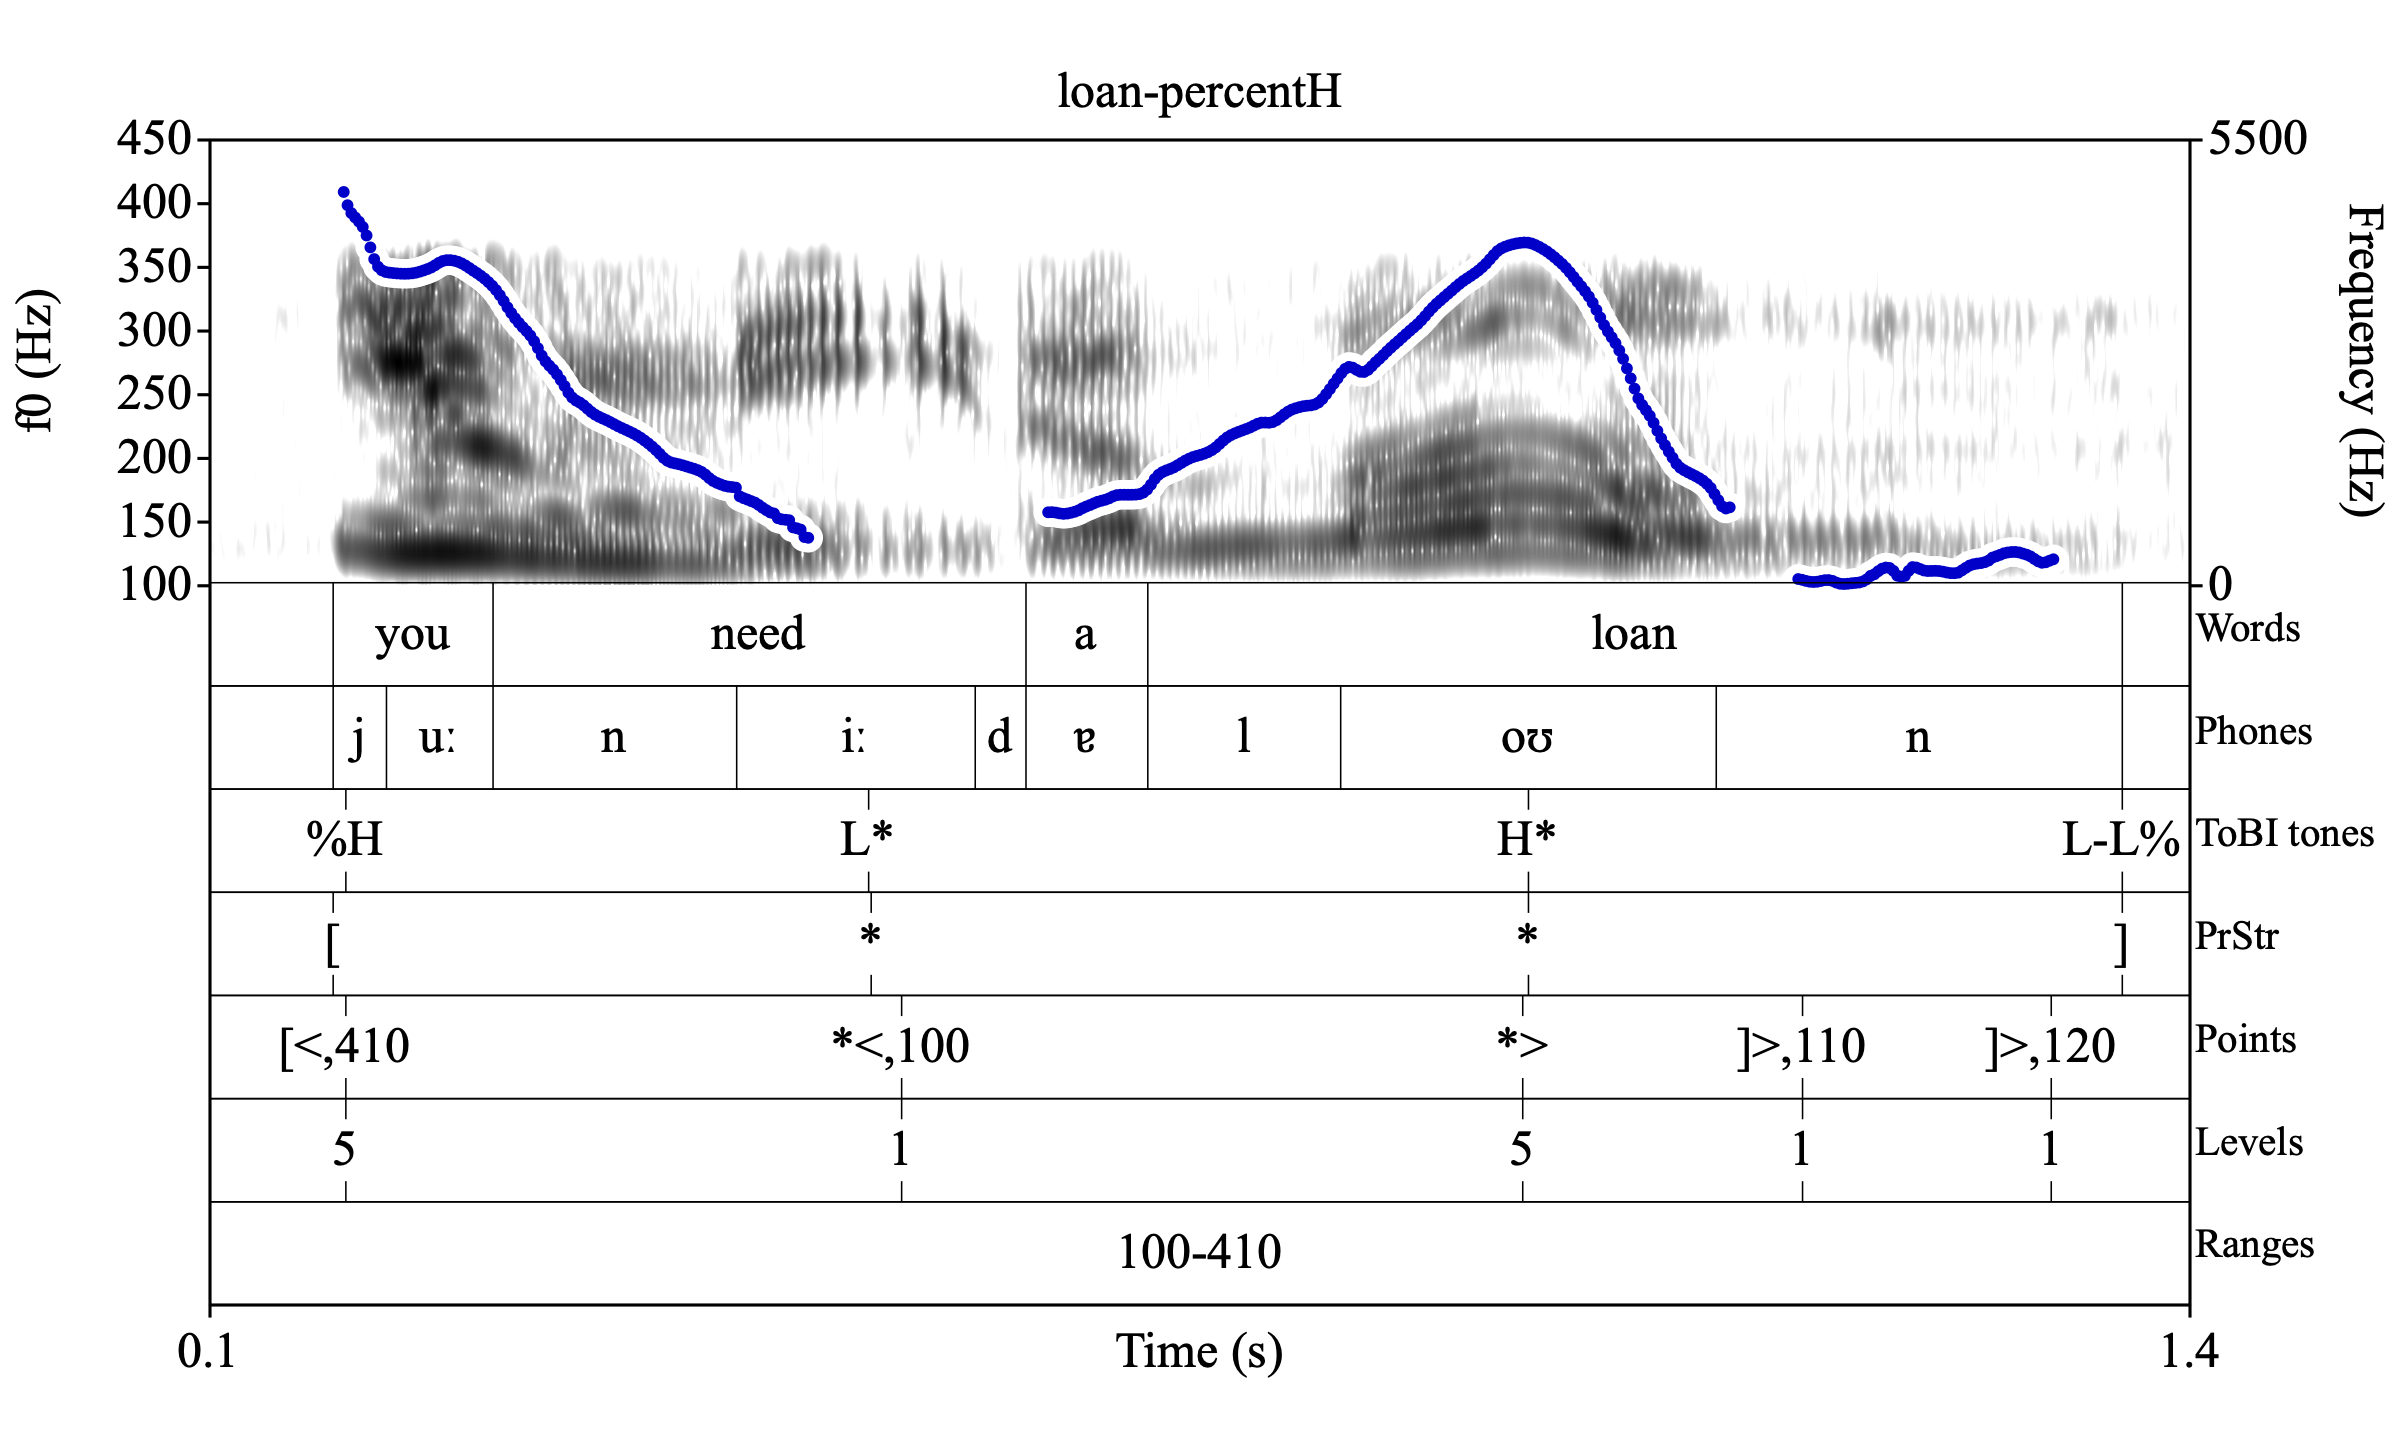
\includegraphics[width=.875\linewidth]{Points-loan-percentH-adv.png}
%
\caption[An initial high-f0 turning point is given a \textlabel{[<} label in the Points tier.]{An initial high-f0 turning point is given a \textlabel{[<} label in the Points tier, indicating affiliation with the \textlabel{[} object in the PrStr tier.%
\label{fig:loan-percentH Points Adv}%
\index{Annotated example, Points tier (advanced)!loan-percentH}
}
\end{figure}

As with other ambiguous cases as described above, there may be times when the signal is ambiguous, so that where there is a high f0 at the beginning of a phrase, a labeller may be uncertain whether there is a prominence or not. In such cases, the labeller can capture this ambiguity with a label such as \textlabel{[</*<} (accompanying, for example  a \textlabel{[} and \textlabel{?*} in the PrStr tier.), as is shown in Figure \ref{fig:honorariums Points Adv}.  This label indicates that the high initial f0 may be associated with either the left boundary, the prominence, or both.

\begin{figure}[H]
\centering
%
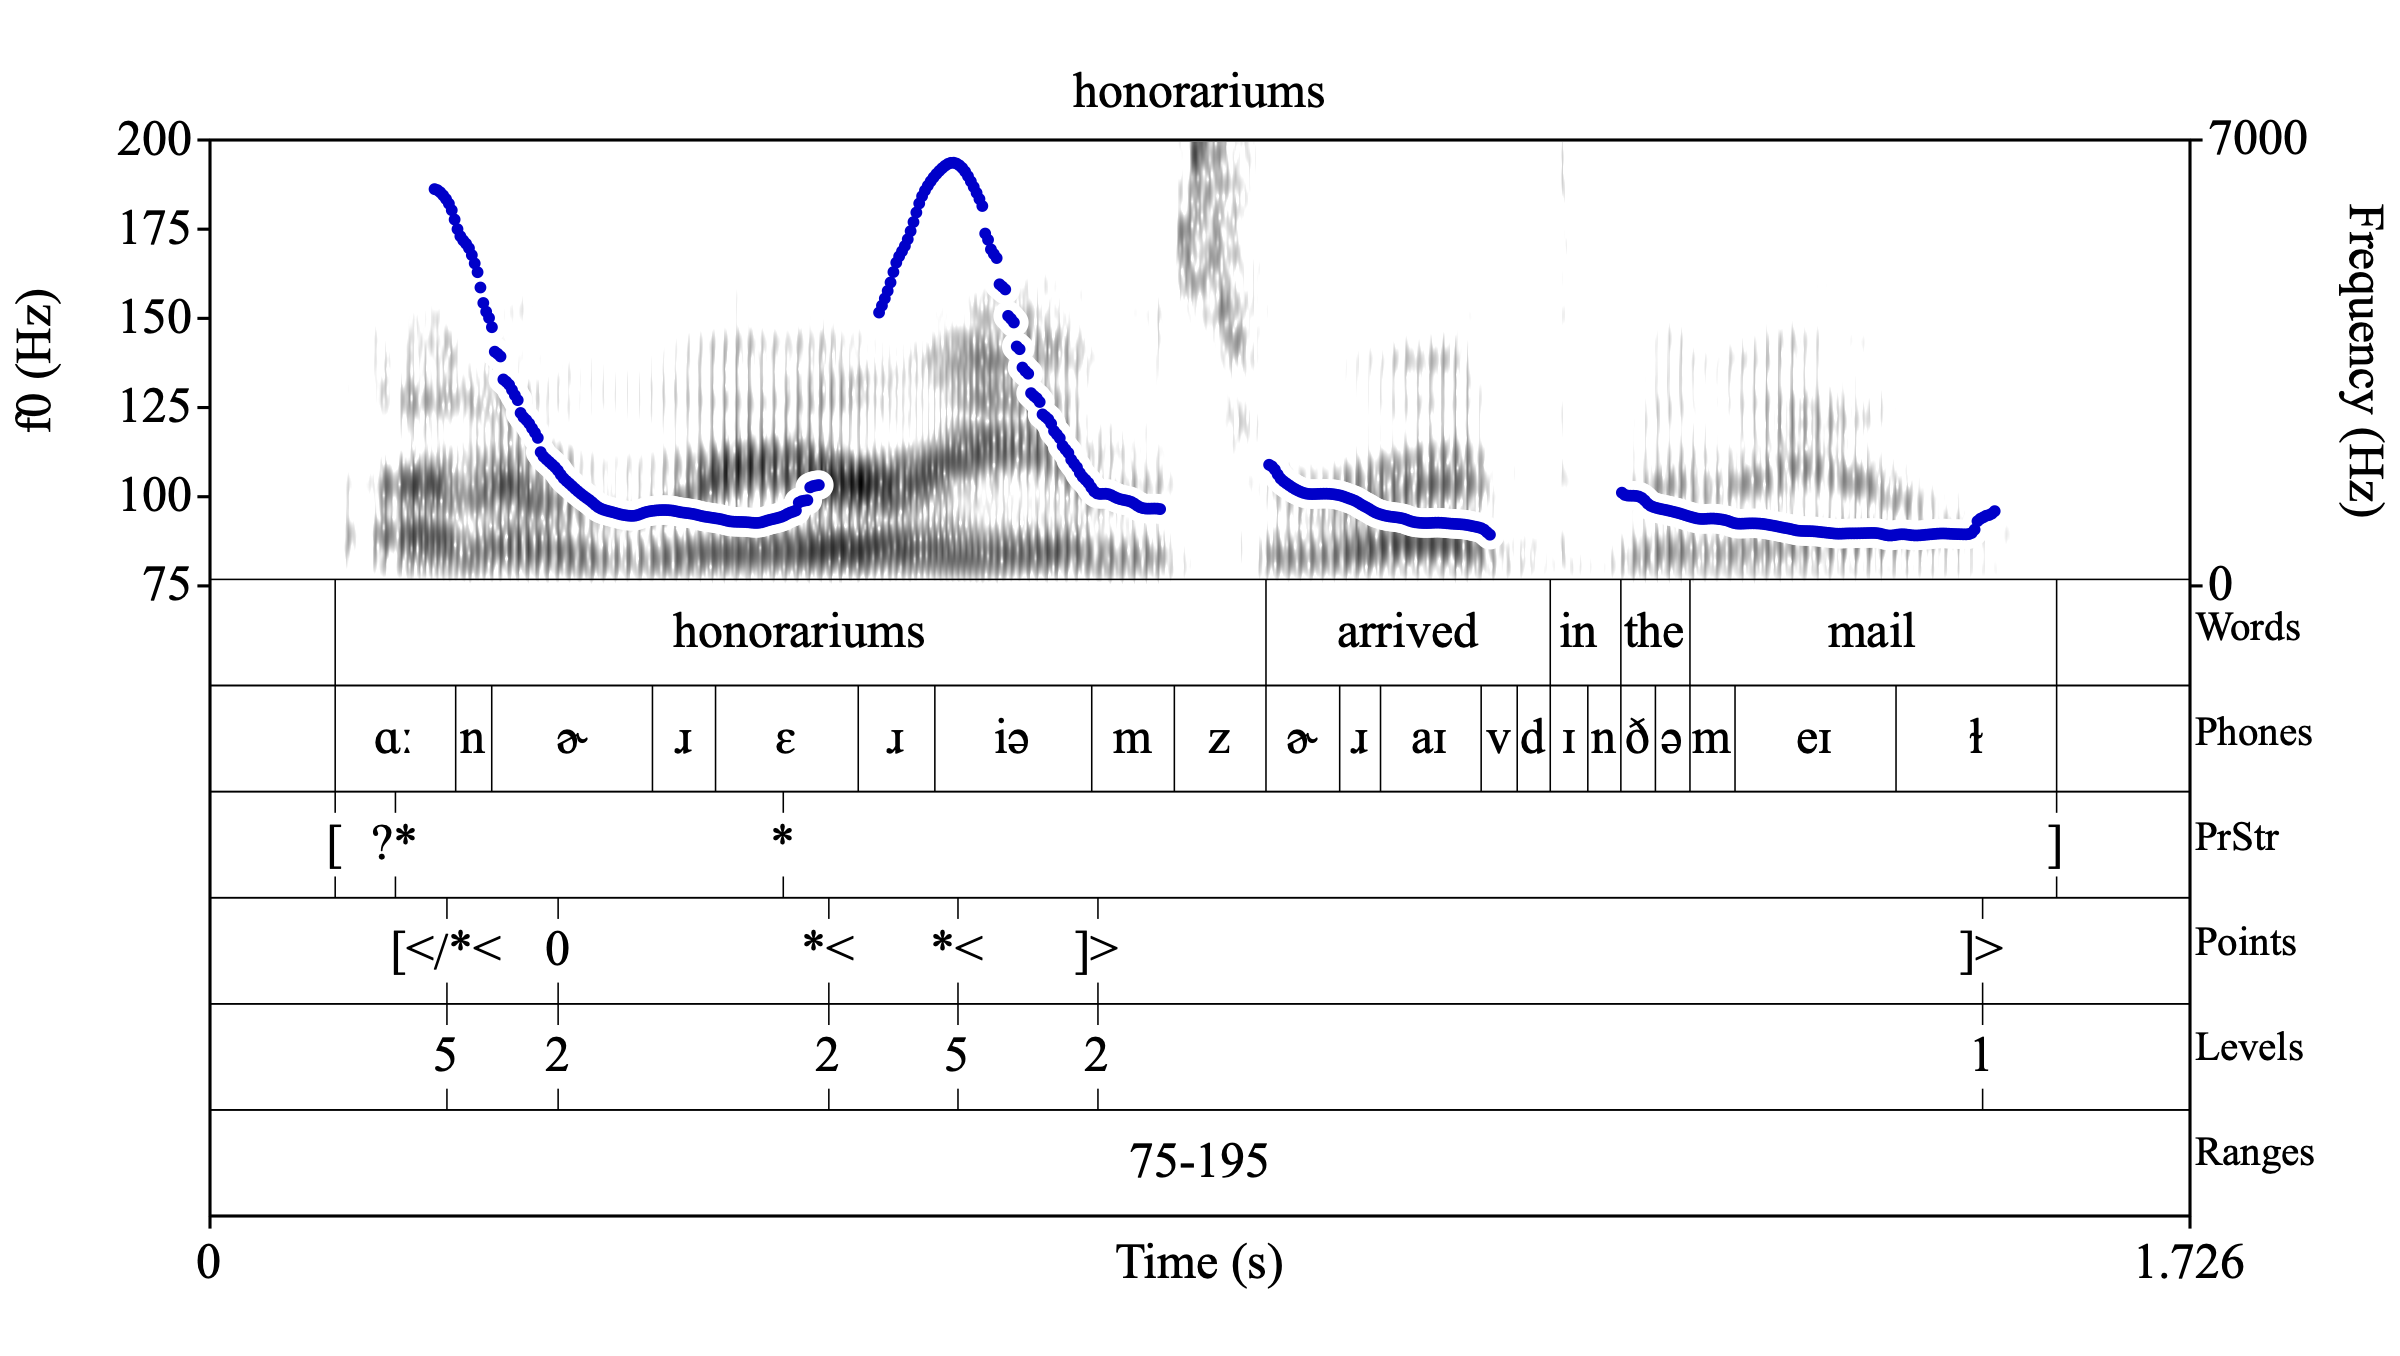
\includegraphics[width=.875\linewidth]{Points-honorariums-adv.png}
%
\caption[An initial high-f0 turning point is given the label \textlabel{[</*<} label in the Points tier.]{An initial high-f0 turning point is given the label \textlabel{[</*<} label in the Points tier, indicating that the labeller considers the affiliation ambiguous between an initial phrase boundary and a potential prominence, labelled \textlabel{[} and \textlabel{?*} (respectively) in the PrStr tier.%
\label{fig:honorariums Points Adv}%
\index{Annotated example, Points tier (advanced)!honorariums}
}
\end{figure}

Researchers using PoLaR may opt to attribute any initial f0 points to phrase beginnings. The example \texttt{vegetable\_list} from Section \ref{sec:phrase-initial-boundaries} is repeated here in Figure \ref{fig:vegetable list Points left edge Adv} with Advanced Points tier labels indicating that initial f0 points are being attributed to the beginnings of each phrase.

\begin{figure}[H]
\centering
%
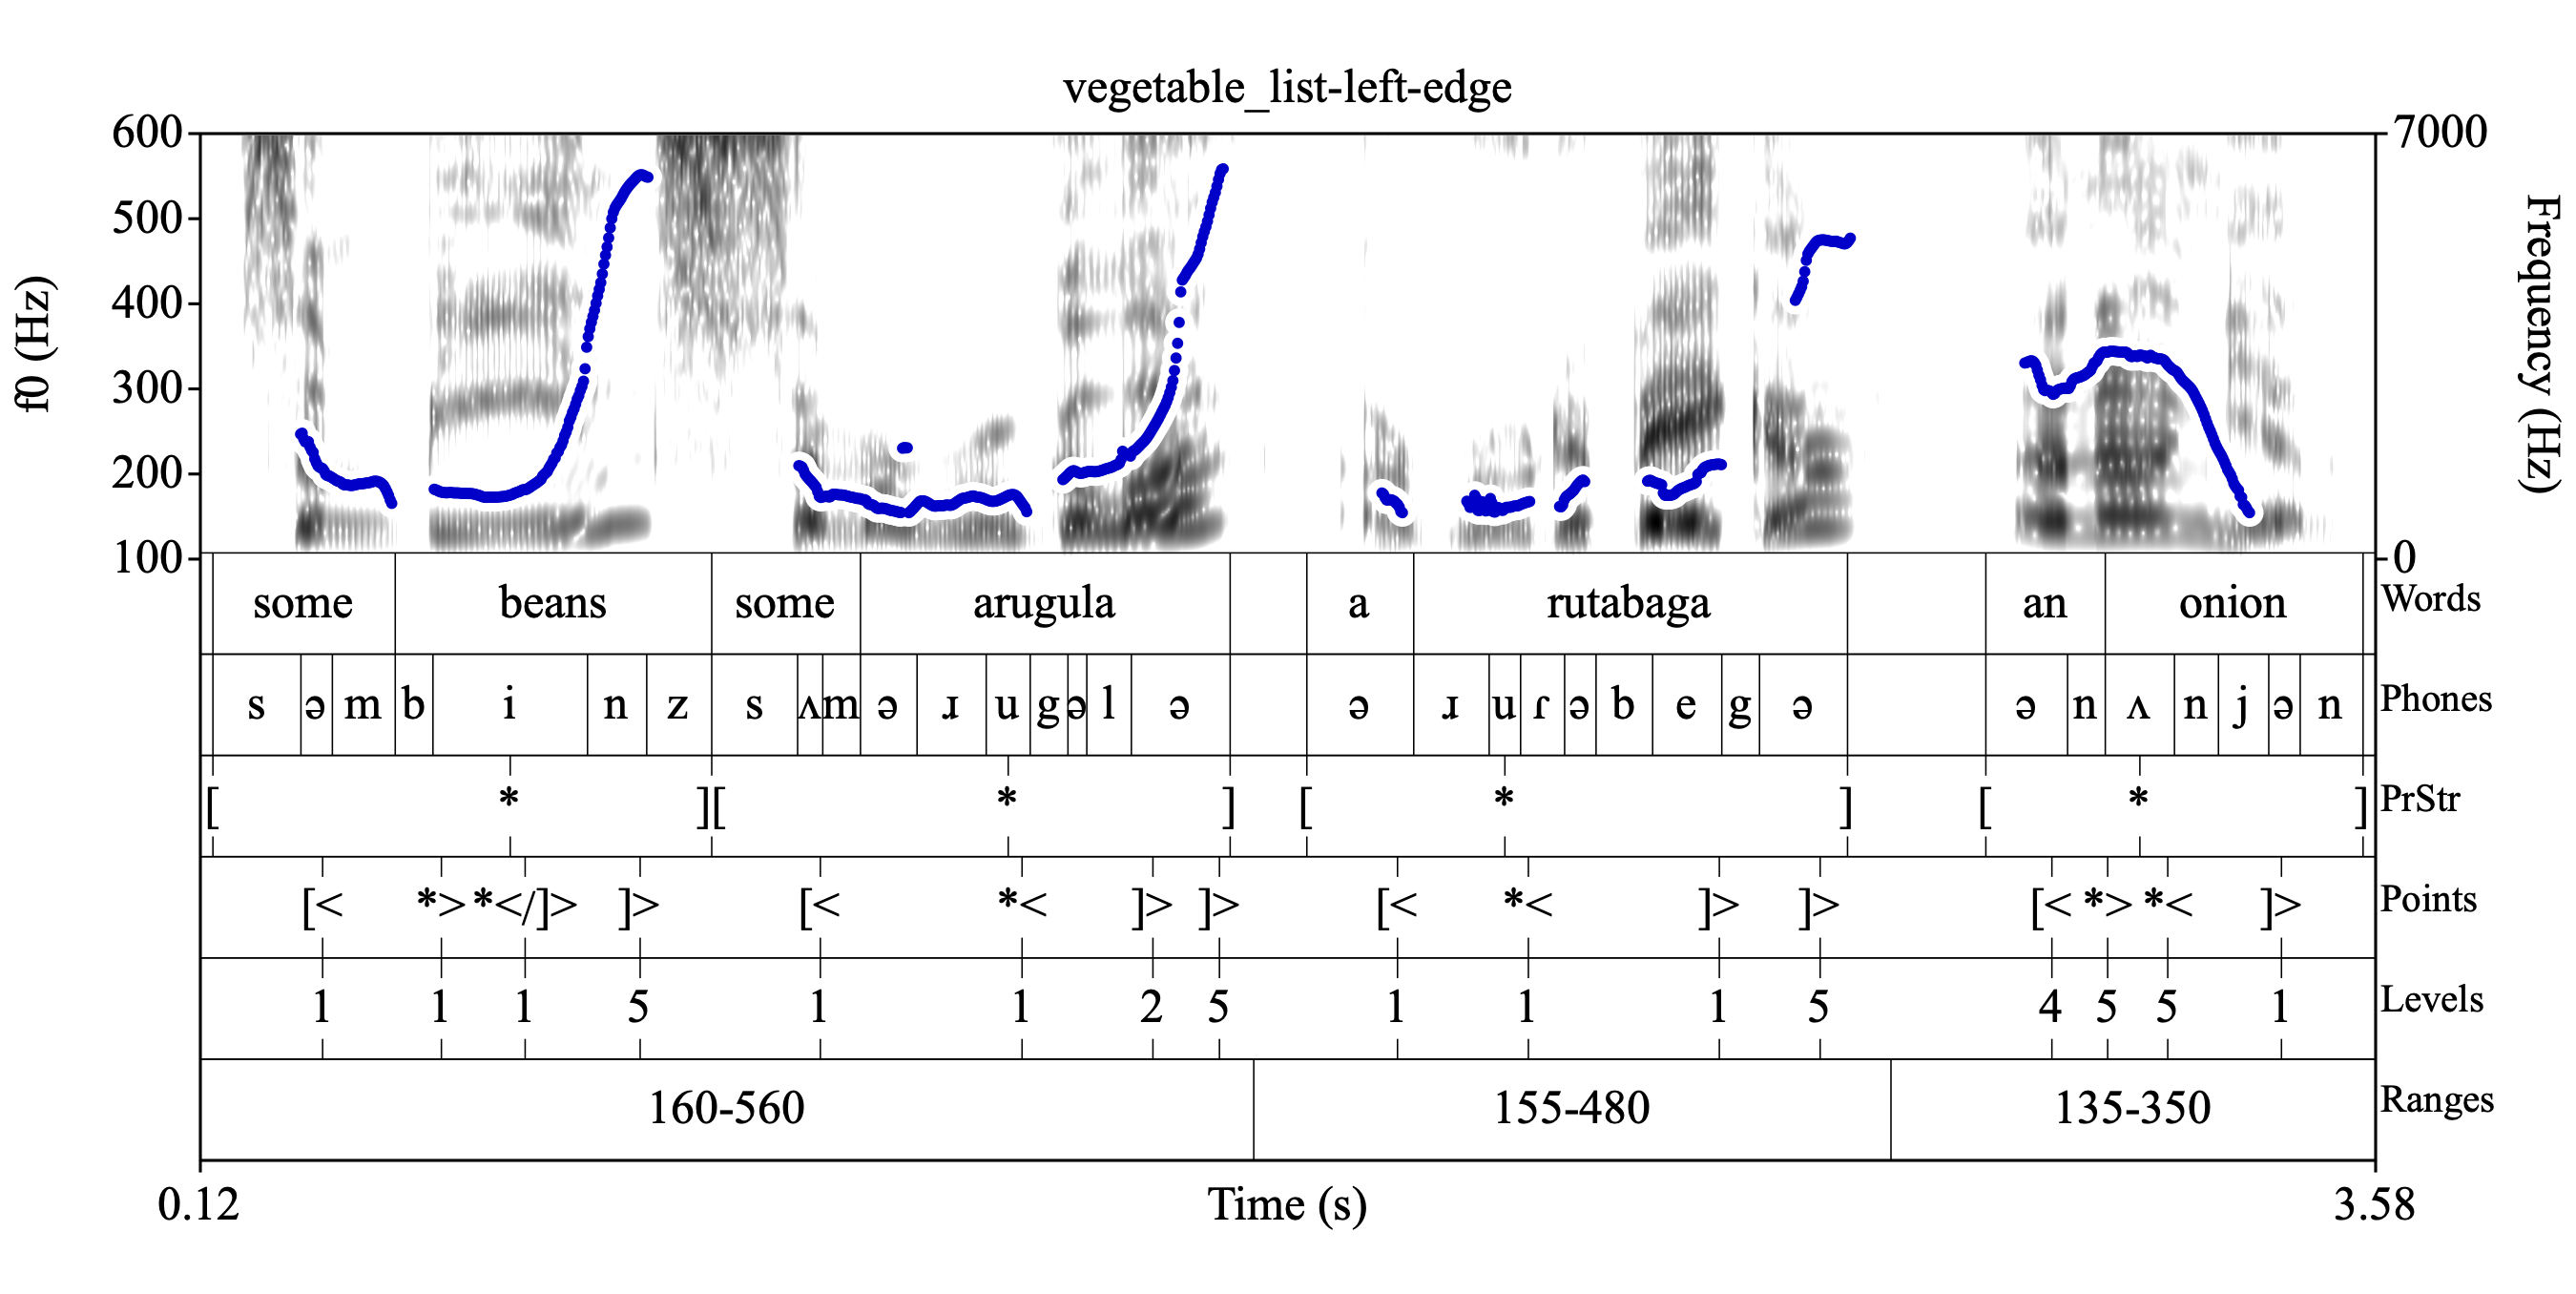
\includegraphics[width=.875\linewidth]{Points-vegetable_list-left-edge.png}
%
\caption[Advanced Points tier labels here indicate that the labeller associates f0 points with phrase ends or beginnings.]{The example \texttt{vegetable\_list} repeated from \S\ref{sec:phrase-initial-boundaries}, with both phrase beginnings and ends annotated in the PrStr tier. Advanced Points tier labels here indicate that the labeller associates f0 points with phrase ends or beginnings.%
\label{fig:vegetable list Points left edge Adv}%
\index{Annotated example, Points tier (advanced)!vegetable\_list}
}
\end{figure}


\subsection{More Examples of Advanced Points Tier Labels}\label{sec:more-examples-of-advanced-points-tier-labels}

When using Advanced labels, it is important for prosodic labellers to be systematic so that data can be retrieved and aggregated with similar contexts or compared against contrasting contexts. Here, we present a series of examples to help annotators establish and internalize the PoLaR system with respect to Points labelling.

The next two examples both contain prominence-related rises, and Example 2 also contains a boundary-related rise. Those labellers with some familiarity with English intonational phonology may have strong intuitions about which phonological event (on the PrStr tier) each of these rises is associated with. The Advanced PoLaR Points labels attempt to capture these intuitions.

\paragraph{Advanced Points Example 1: Points and PrStr}
First, examine this example of turning points in the pitch track each associated with distinct objects in the Prosodic Structure tier:

\begin{figure}[H]
\centering
%
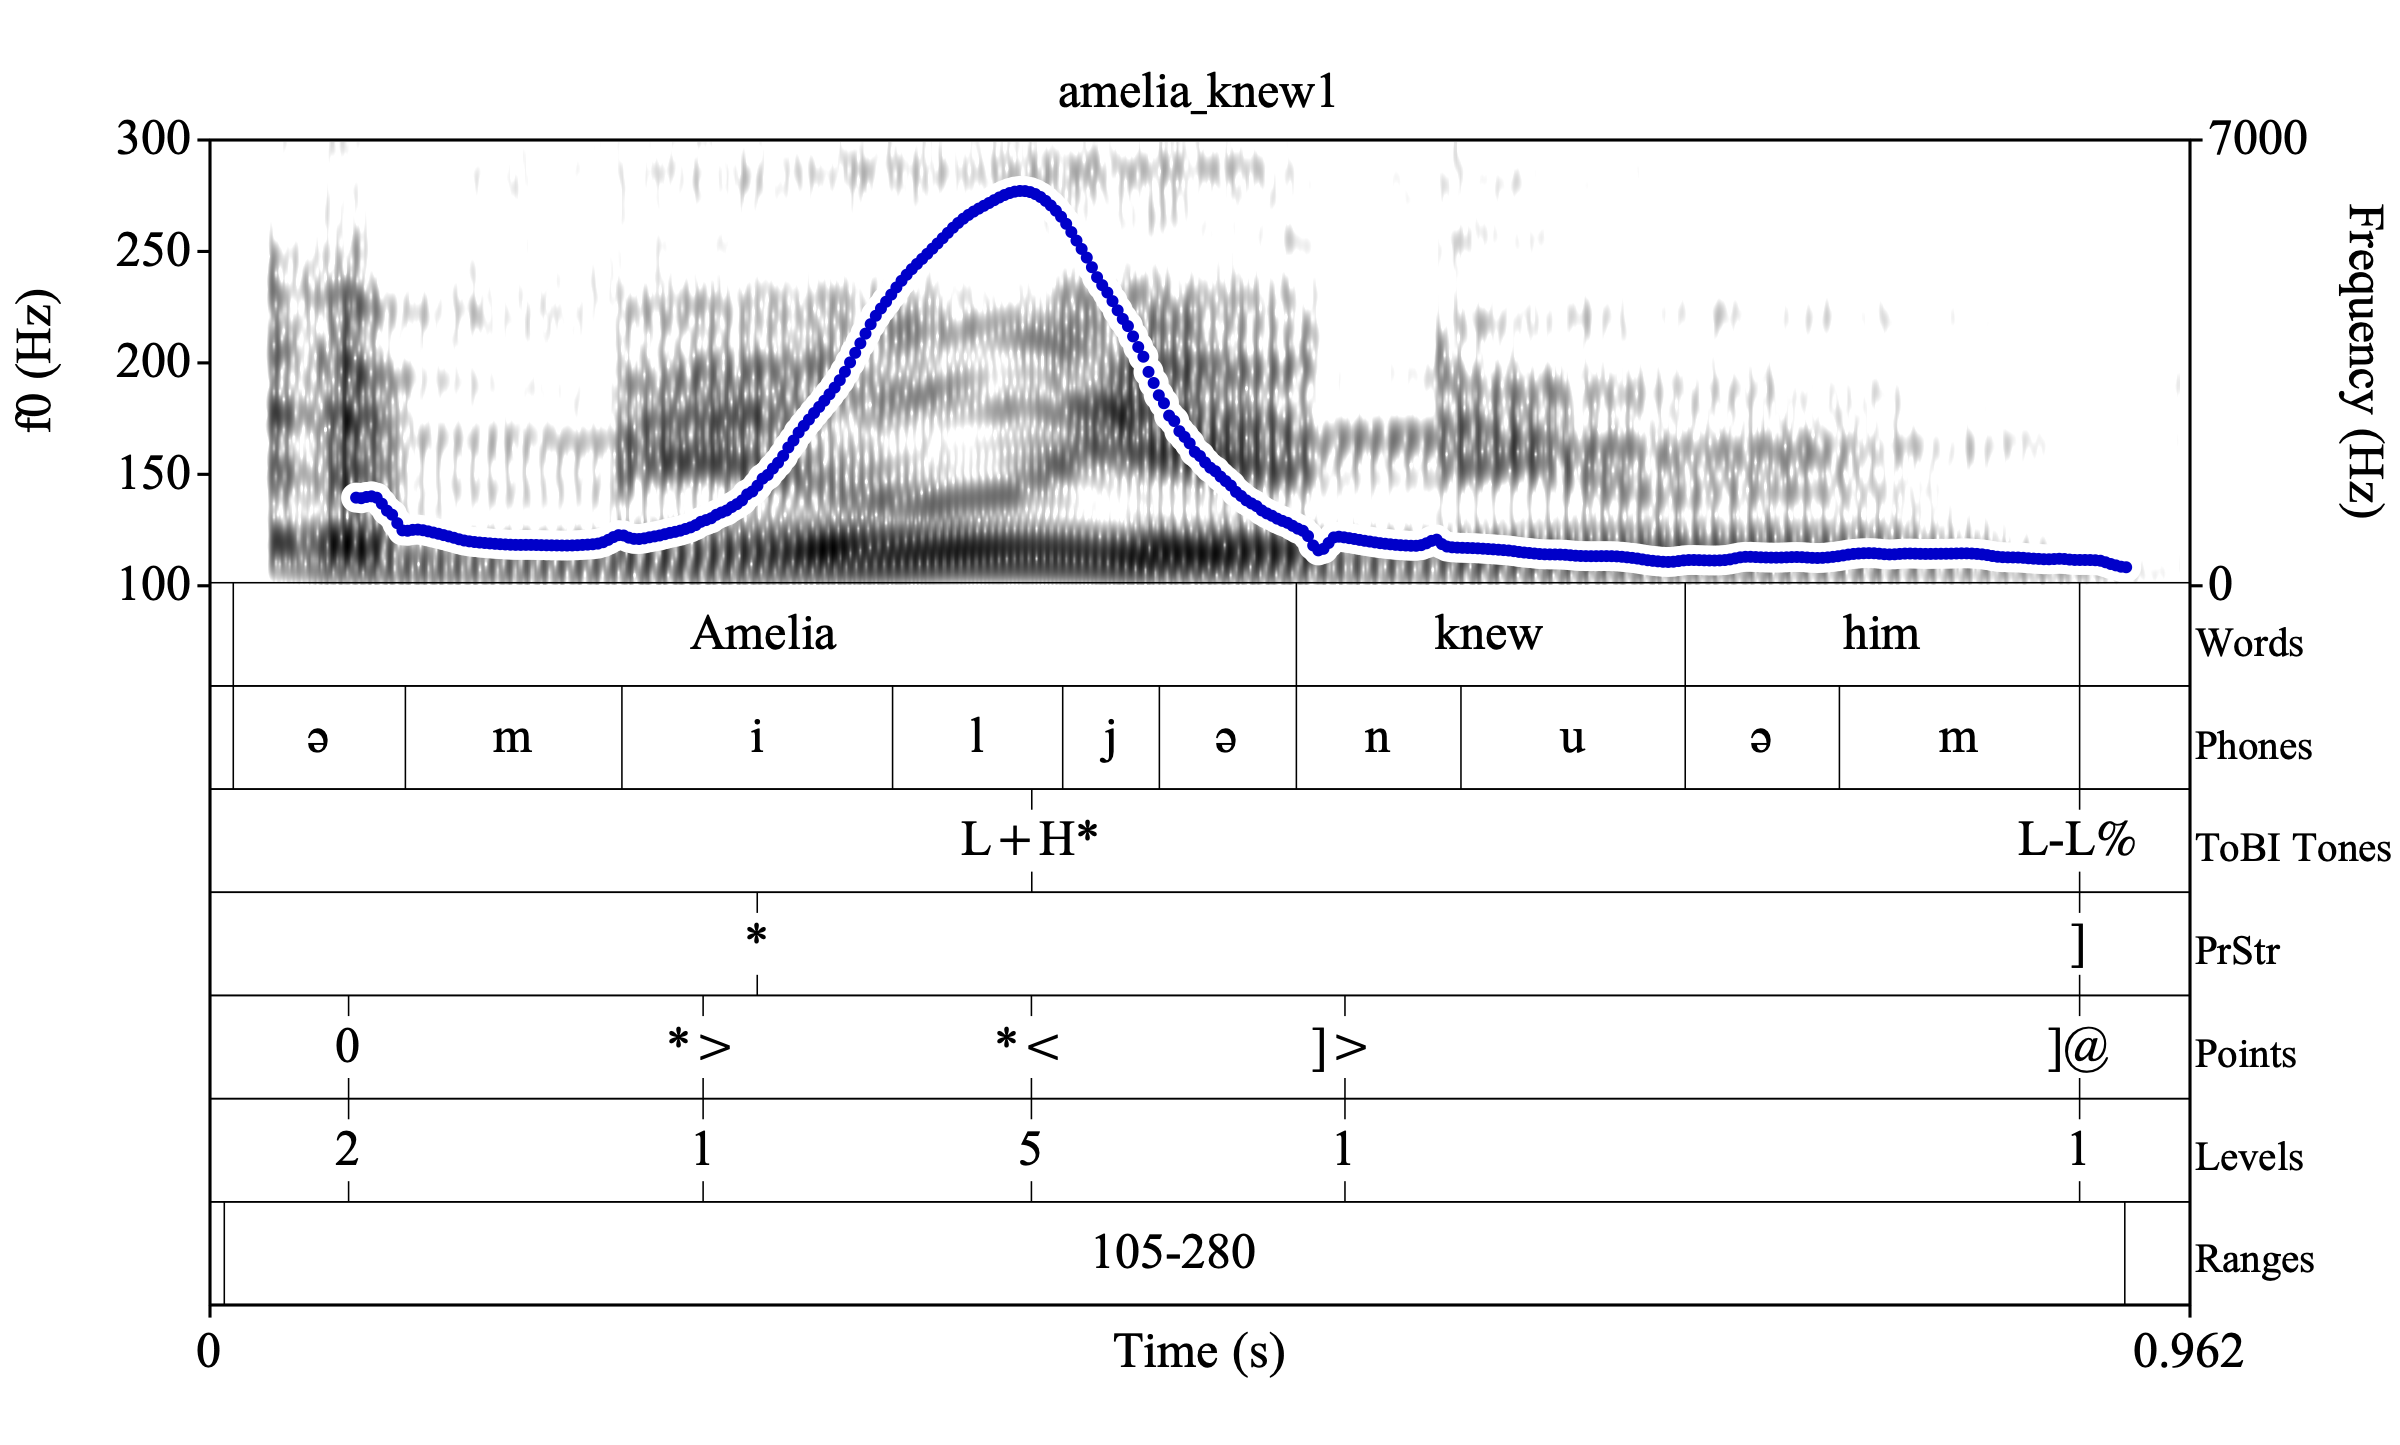
\includegraphics[width=.875\linewidth]{Points-amelia_knew1-adv.png}
%
\caption{\texttt{amelia\_knew1}, with Advanced PoLaR labels.%
\label{fig:amelia_knew1 Points Adv}%
\index{Annotated example, Points tier (advanced)!amelia\_knew1}
}
\end{figure}

Again there is a single prominent word and the utterance is comprised of a single intonational phrase. In this case, the annotator has labelled the beginning of the reliable pitch with a ‘\textlabel{0}’, indicating they don’t believe this initial pitch is related to any particular PrStr object. Next, the rise in pitch (described with two f0 turning points: one at the base of the rise and one at the peak) is analyzed as being associated with one phonological object: the prominence labelled on the PrStr tier (at the midpoint of [i] vowel in Am\textbf{\uline{e}}lia, as transcribed in the Phones tier). We annotate our analysis (that these two turning points are associated with this single phonological object) by using the ‘\textlabel{*>}’ and ‘\textlabel{*<}’ labels for two Points tier objects. Next, the pitch falls to a steady low, which has been analyzed as related to the phrase boundary labelled on the PrStr tier. The beginning of this steady low is annotated with a ‘\textlabel{]>}’ label. The end of this steady low has been annotated with a ‘\textlabel{]@}’ label: the ‘\textlabel{]}’ label on the PrStr tier and the f0 turning point on the Points tier are positioned at the same point in time, and so a @ pointer is used (instead of the more common ‘\textlabel{>}’ or ‘\textlabel{<}’).

\paragraph{Advanced Points Example 2: A minimal pair with above}
This example differs minimally from the one above: there are two rises in pitch. The first is related to the prominence (as before), but there is a second rise related to the phrase boundary.

\begin{figure}[H]
\centering
%
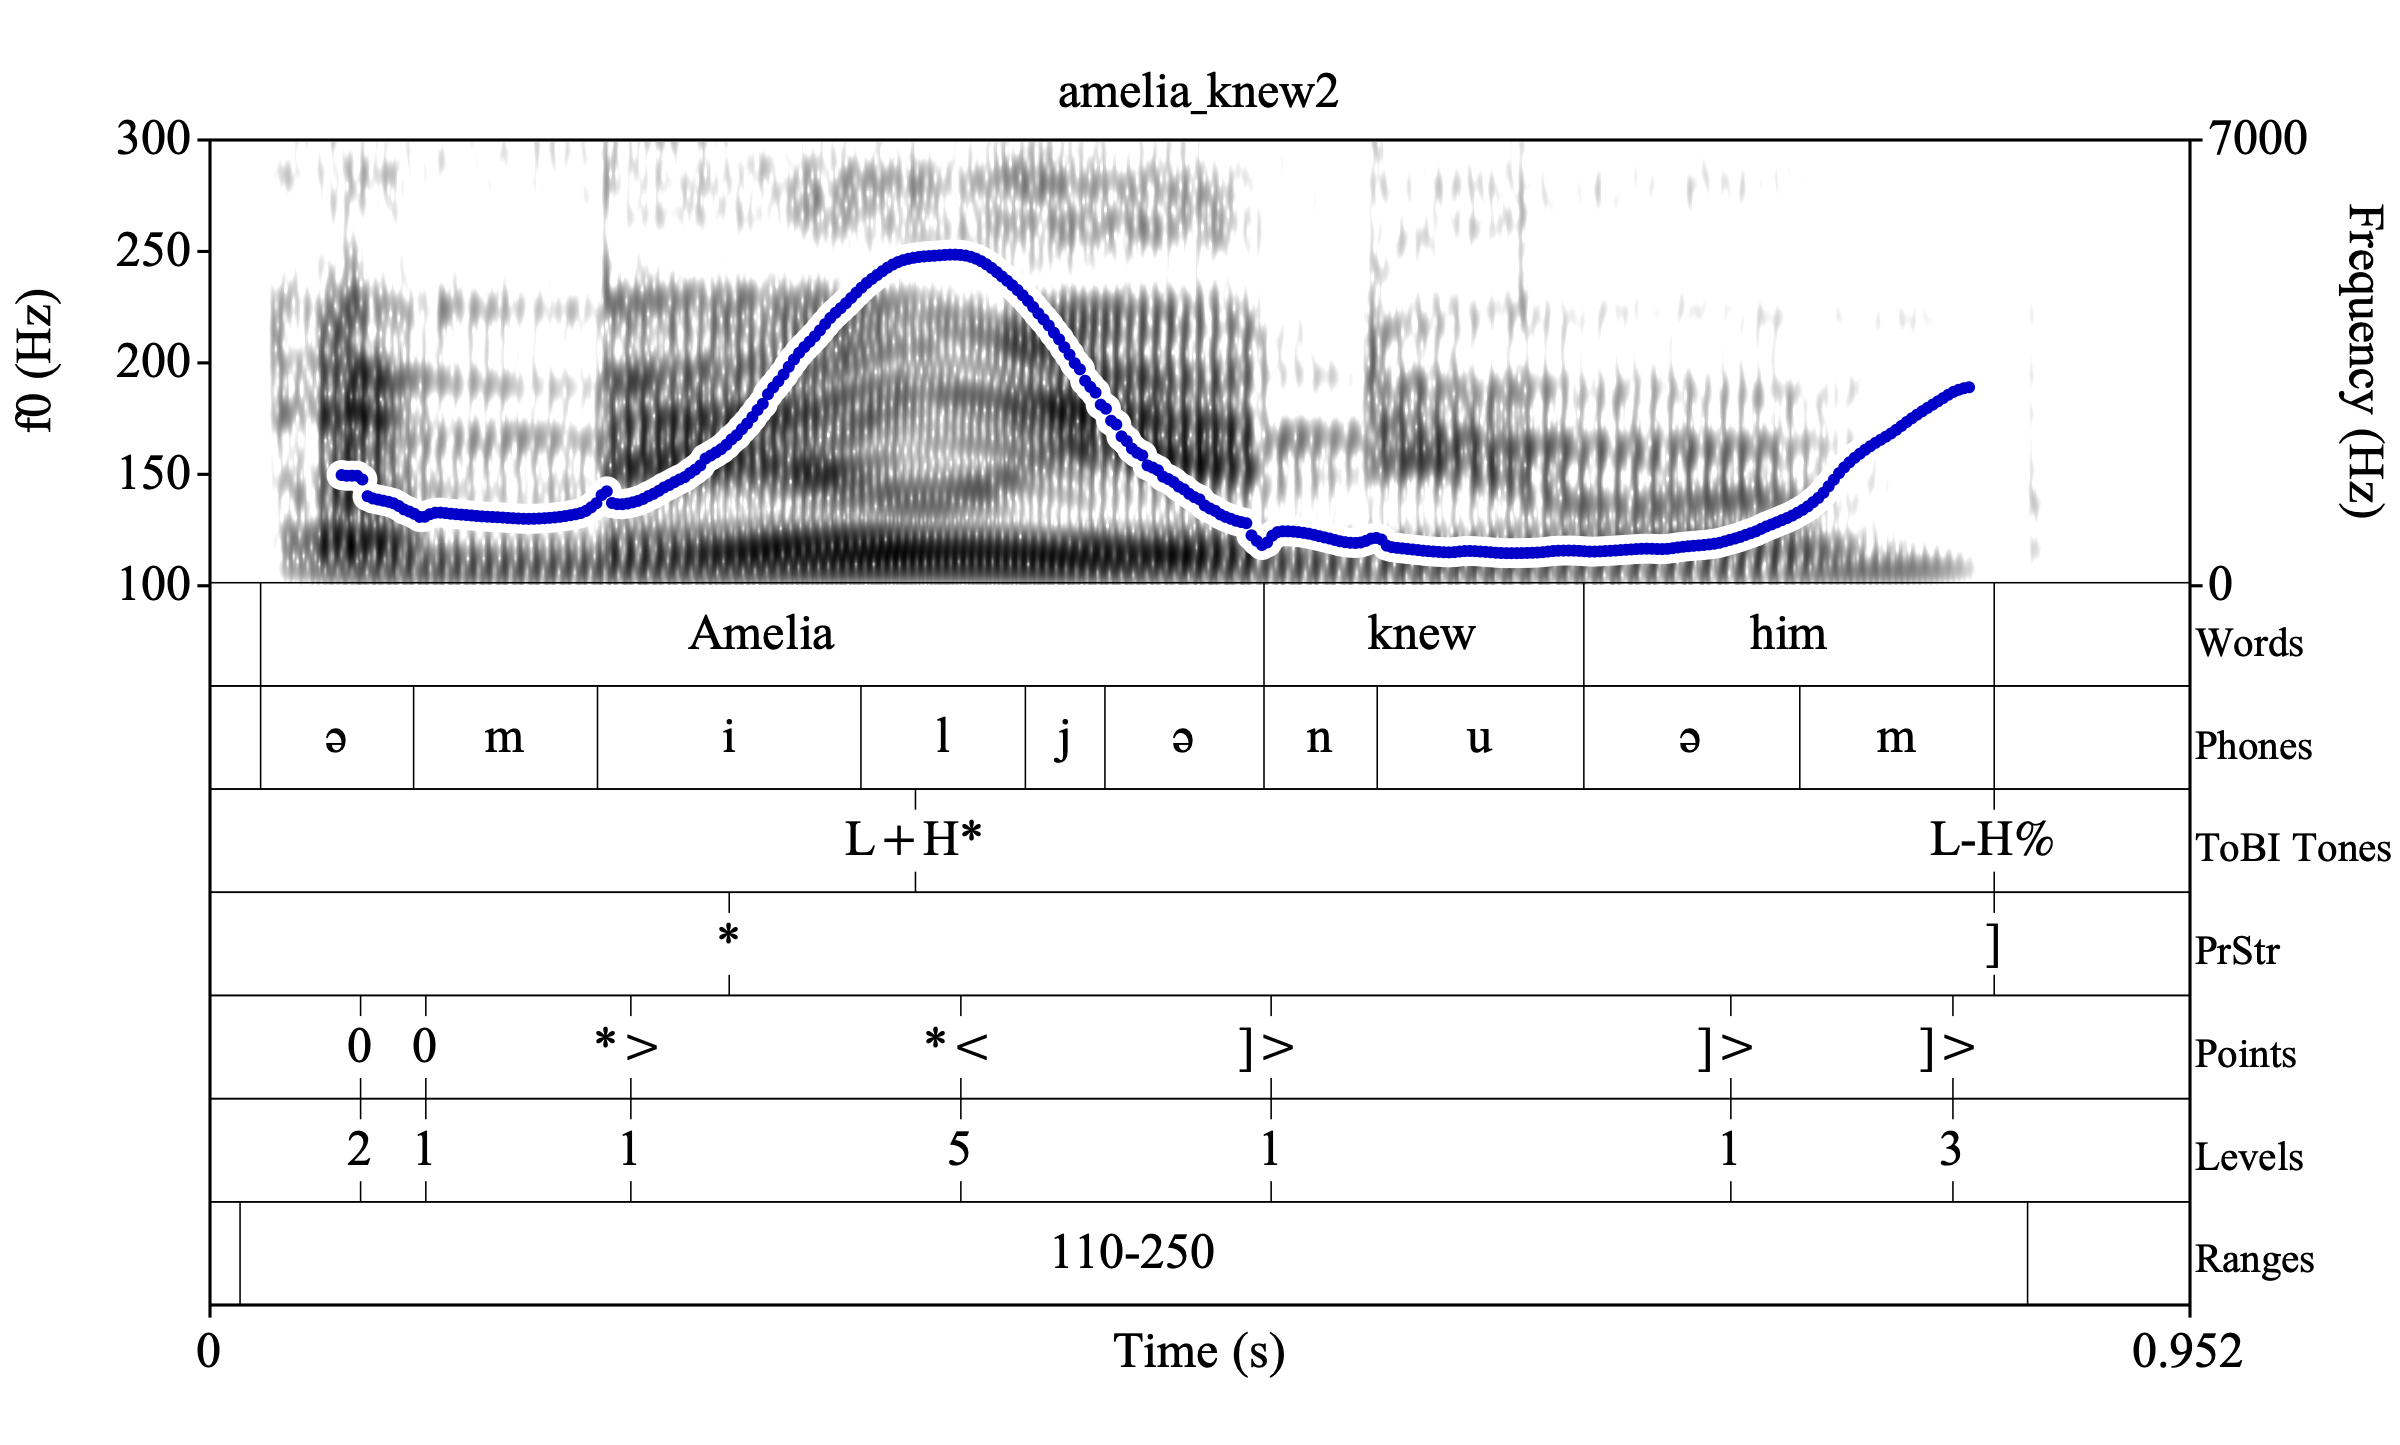
\includegraphics[width=.875\linewidth]{Points-amelia_knew2-adv.png}
%
\caption{\texttt{amelia\_knew2}, with Advanced PoLaR labels.%
\label{fig:amelia_knew2 Points Adv}%
\index{Annotated example, Points tier (advanced)!amelia\_knew2}
}
\end{figure}

In this example, three ‘\textlabel{]>}’ labels are used. The first two bookend the low plateau, and the third is for the endpoint of the final rise. By assigning all three of these movements ‘\textlabel{]>}’ labels, the labeller indicates that they analyze the low plateau and the final mid rise as all related to the phrase-final boundary. Thus, PoLaR provides a means for a labeller to distinguish boundary-related rises and prominence-related rises.

\paragraph{Advanced Points Example 3: Ambiguous signal}
As mentioned above, there are also cases where the signal might be ambiguous, such that a labeller could find support for an analysis where a rise may be a sort of ‘trailing tone’ for a previous pitch accent, or a ‘leading tone’ for a following pitch accent. An example of this is shown in Figure \ref{fig:sara_murray Points Adv}.

\begin{figure}[H]
\centering
%
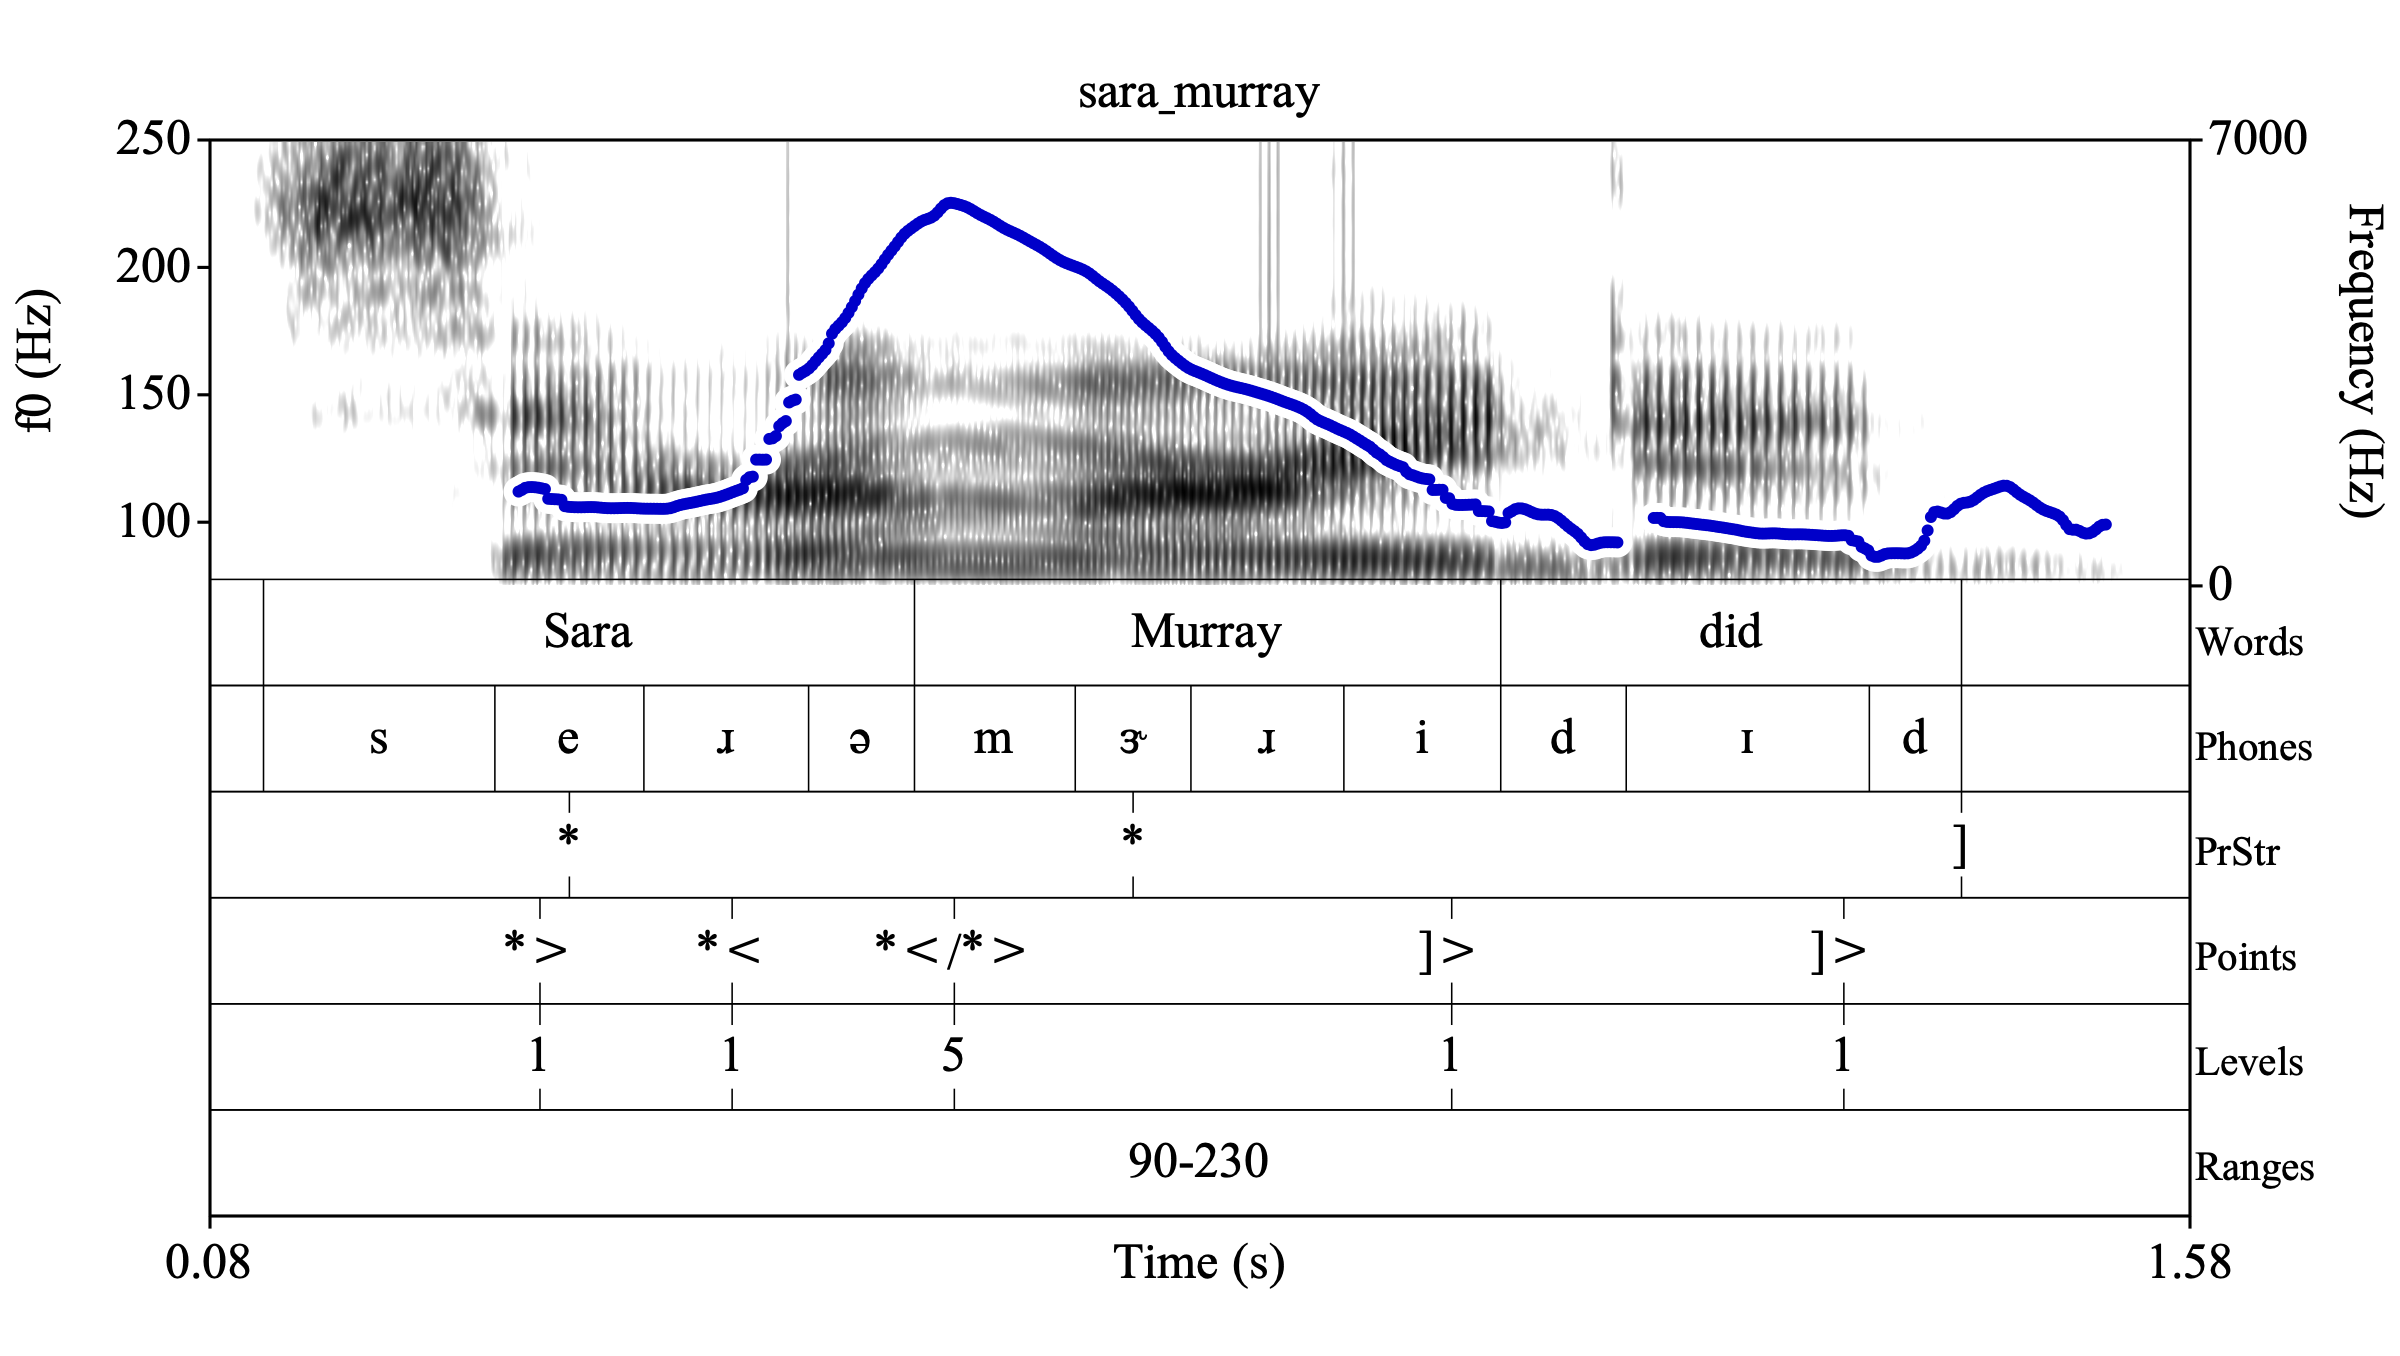
\includegraphics[width=.875\linewidth]{Points-sara_murray-adv.png}
%
\caption{\texttt{sara\_murray}, with Advanced PoLaR labels.%
\label{fig:sara_murray Points Adv}%
\index{Annotated example, Points tier (advanced)!sara\_murray}
}
\end{figure}

As in the previous examples, most turning points can be analyzed as being associated with PrStr events. Turning points 1 and 2 are associated with the low pitch accent on \langtext{Sara} and the last two turning points are associated with the phrase boundary. However, the label on the 3rd point, ‘\textlabel{*</*>}’, indicates that this turning point is possibly associated with the preceding pitch accent (‘\textlabel{*<}’; i.e., \langtext{Sara} is associated with a late-rising pitch accent), with the following pitch accent (‘\textlabel{*>}’; i.e., \langtext{Murray} is associated with an early-falling pitch accent), or possibly even both (as a kind of coalescence). Finally, the 4th and 5th turning points, both labelled ‘\textlabel{]>}’, indicate that the labeller hears the word \langtext{did} as flat, with this plateau as cues to the phrase-final boundary. Before continuing on, one might note that there appears to be a visible shift in the slope of the fall curing the [ɹ] of \langtext{Murray}. To see if this should be labelled as a turning point in the intonational contour, one can use straight-line approximation methods to attempt resolve the uncertainty (e.g., pitch manipulation, as discussed in section \ref{sec:intonational-contours-and-software-based-pitch-tracks} of Chapter \ref{ch:basics}. However, the results might not be definitive – in such a case, a labeller can use the \textlabel{?0} label where they believe there may be a pitch turning point. (A labeller might also choose to postpone using the algorithm until later, and until this point is using \textlabel{?0} as a kind of placeholder.)

\paragraph{Advanced Points Example 4: A minimal pair with above}
In the previous example, \texttt{sarah\_murray}, there is a turning point that could be interpreted as cuing the \textlabel{*} on \langtext{Sara} or the \textlabel{*} on \langtext{Murray}. Compare that with what might be perceived as “the same” intonational contour, overlaid on a slightly longer utterance – one with an additional unstressed between the stressed syllables of \langtext{Sara} and \langtext{Murray}:

\begin{figure}[H]
\centering
%
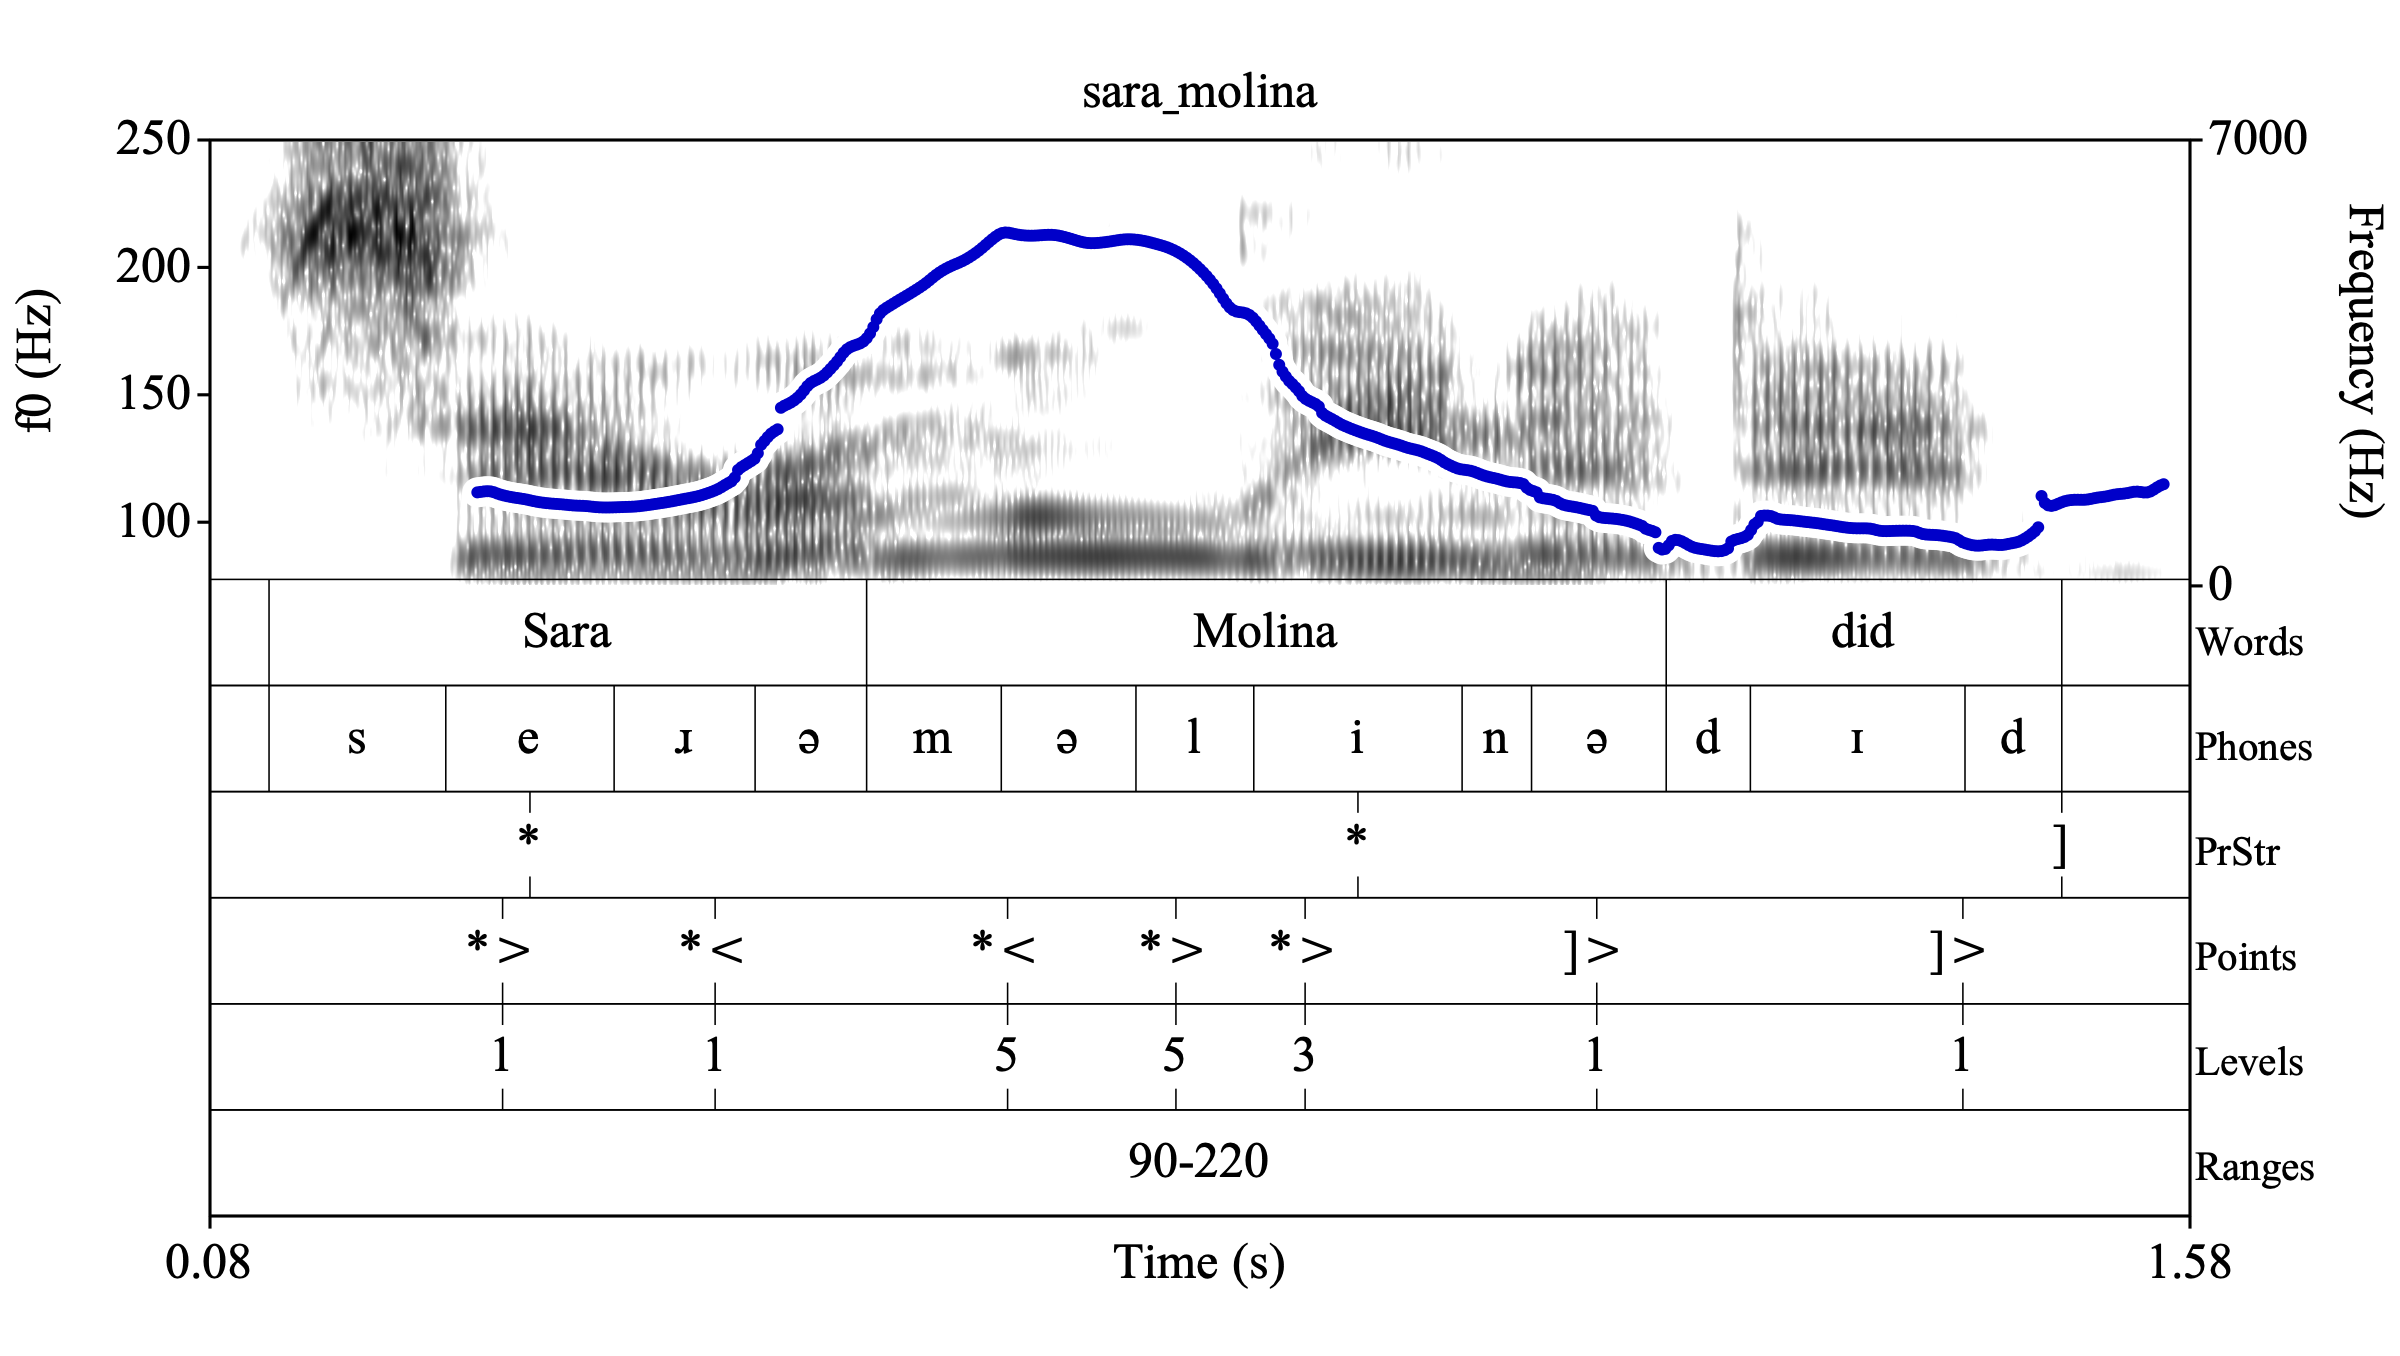
\includegraphics[width=.875\linewidth]{Points-sara_molina-adv.png}
%
\caption{\texttt{sara\_molina}, with Advanced PoLaR labels.%
\label{fig:sara_molina Points Adv}%
\index{Annotated example, Points tier (advanced)!sara\_molina}
}
\end{figure}

In this case, we can see that there is a plateau stretching between the [m] and [l] of \langtext{Molina}. The labeller has indicated an analysis on the Points tier that says the prominence on \langtext{Sara} is a low-high rise (1-1-5, in the Levels labels) and \langtext{Molina} as a high-mid fall (5-3, in the Levels labels). Notably, instead of the ‘\textlabel{*</*>}’ single point in \texttt{sarah\_murray} as in Figure \ref{fig:sara_murray Points Adv}, in this example there are two points ‘\textlabel{*<}’ and ‘\textlabel{*>}’ at the beginning of \langtext{Molina} (where there is ‘more space’ than in \langtext{Murray}). This supports the analysis that the ‘\textlabel{*</*>}’ in \texttt{sarah\_murray} is a kind of coalescence, as suggested in the discussion above.

\paragraph{Advanced Points Example 5: Non-PrStr-related Points labels}
There is always a possibility that a labeller might want to analyze a movement (here, a rise) in pitch that is neither prominence-related nor boundary-related. Such an example is below:\footnote{Note that the fourth Points tier label is ‘\textlabel{*@}’ and not ‘\textlabel{**@}’. The ‘\textlabel{*@}’, ‘\textlabel{*<}’, and ‘\textlabel{*>}’ labels are meant to point at any type of \textlabel{*} label (i.e., ‘\textlabel{*}’, ‘\textlabel{**}’, ‘\textlabel{?*}’) on the Prosodic Structure tier. Similar for ‘\textlabel{]>}’ on the Points tier pointing to a ‘\textlabel{]]}’ on the PrStr tier.}

\begin{figure}[H]
\centering
%
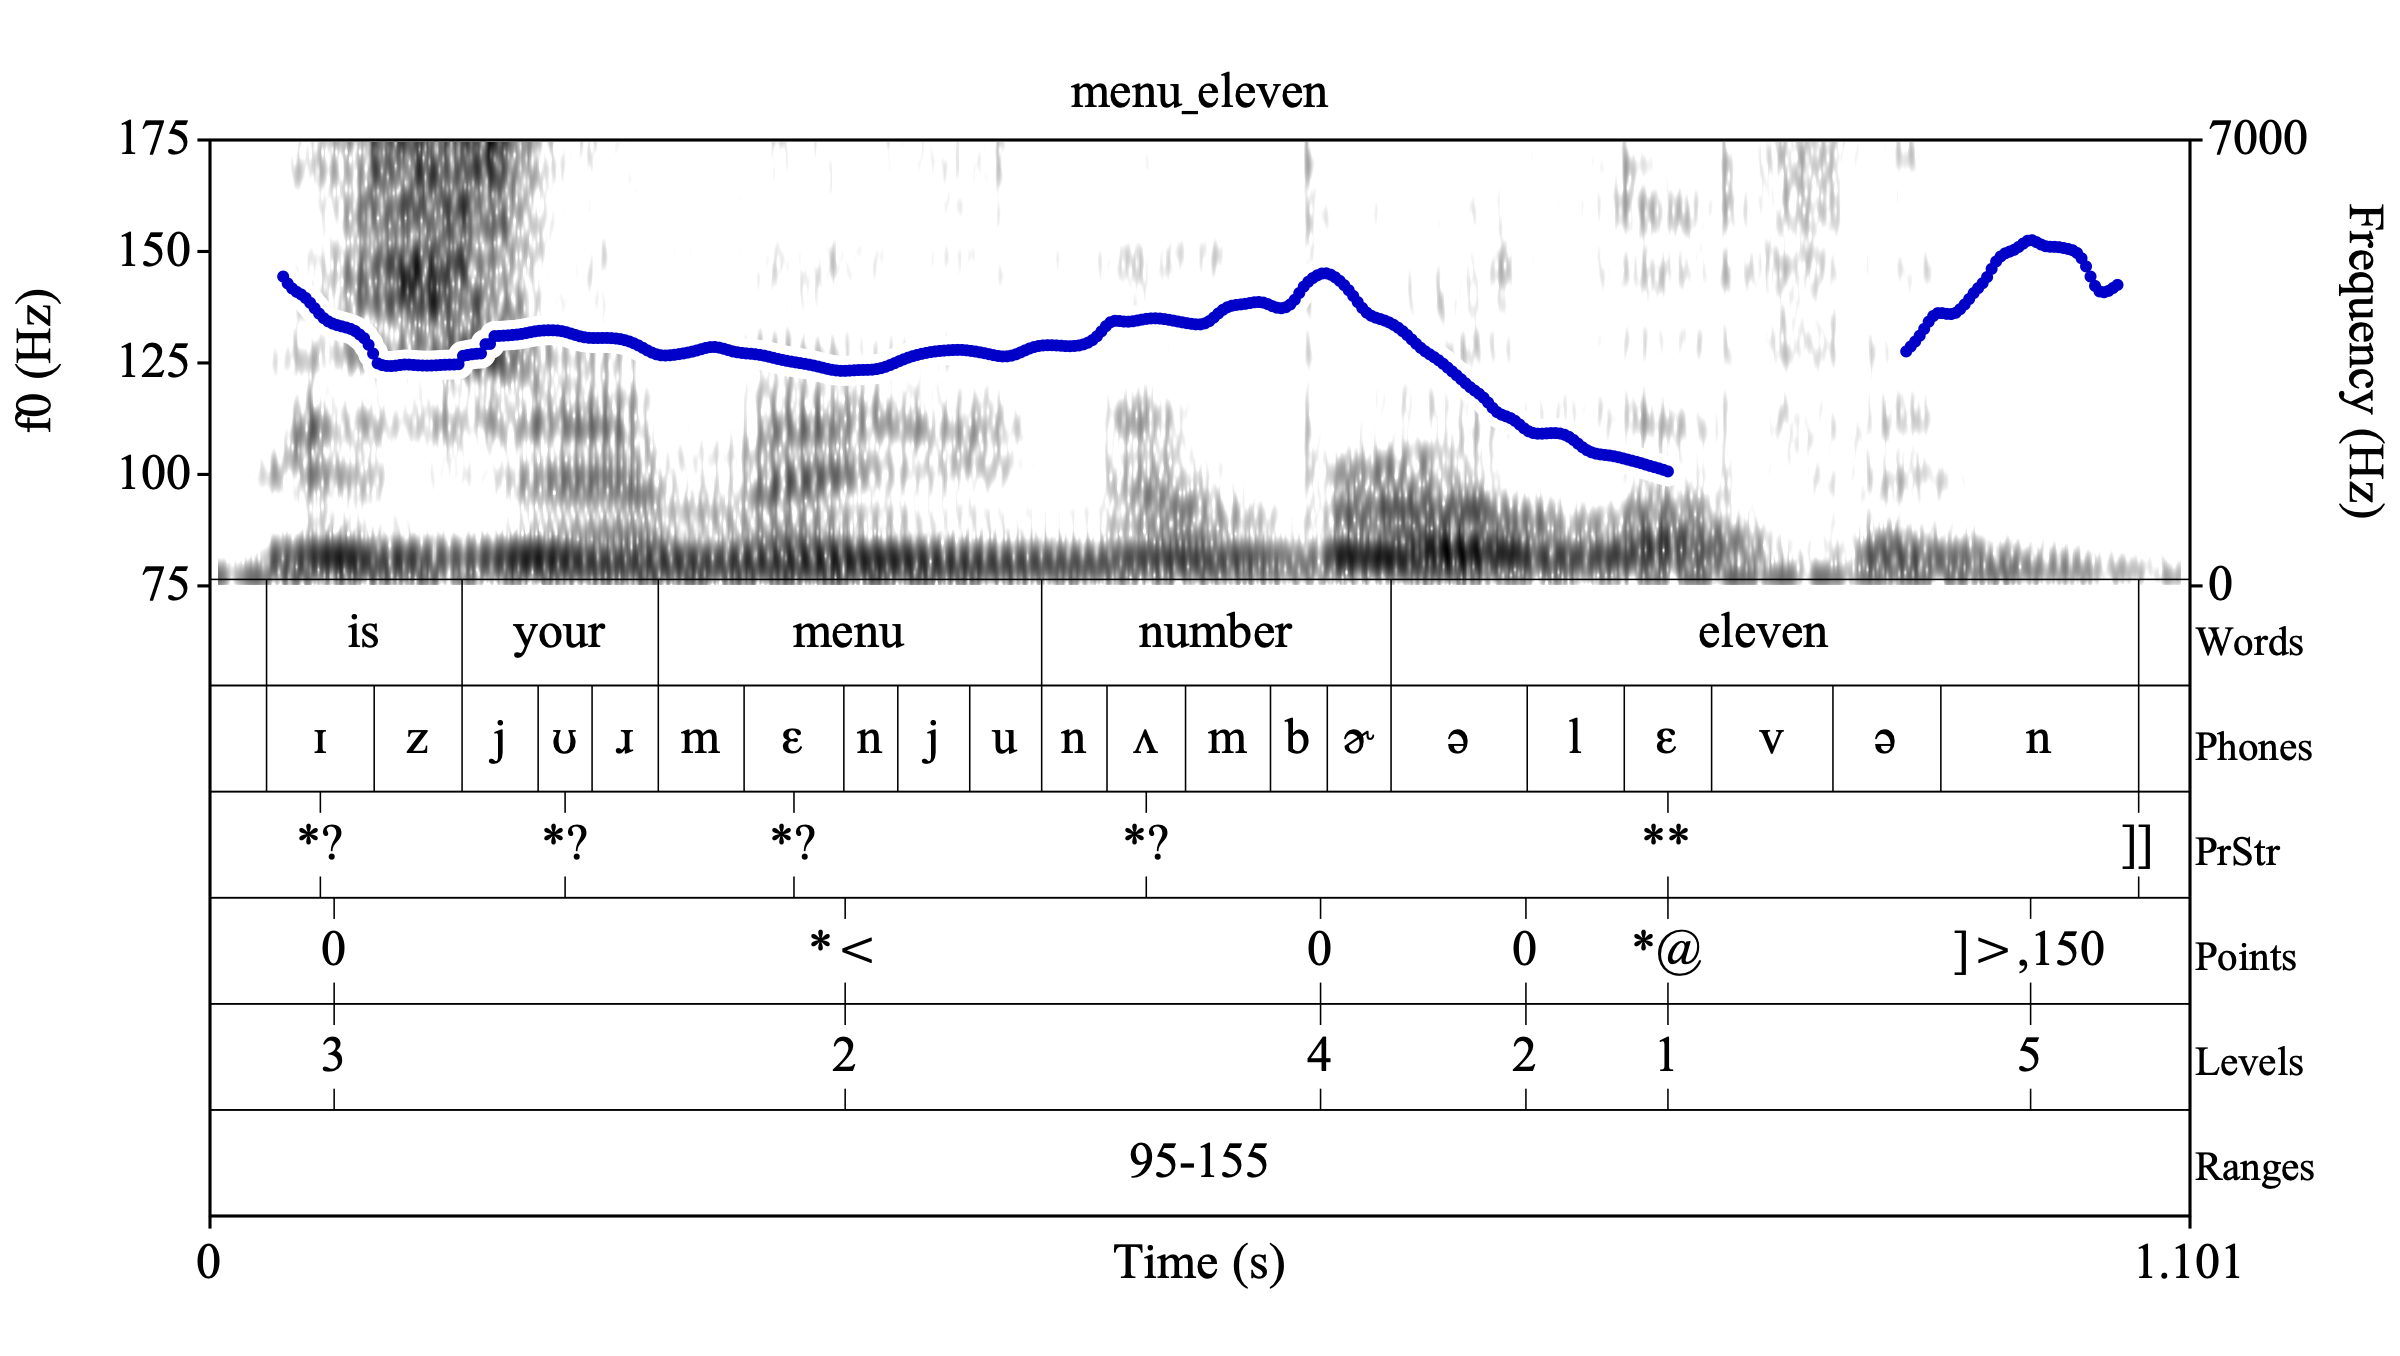
\includegraphics[width=.875\linewidth]{Points-menu_eleven-adv.png}
%
\caption[\texttt{menu\_eleven}, with Advanced PoLaR labels.]{\texttt{menu\_eleven}, with Advanced PoLaR labels. Note the placement of the comma-override label at the end of “\langtext{eleven}”: it comes after the ‘\textlabel{]>}’. %
\label{fig:menu_eleven Points Adv}%
\index{Annotated example, Points tier (advanced)!menu\_eleven}
}
\end{figure}

Since the initial f0 movements at the very beginning of the utterance are not always reliable, a ‘\textlabel{0}’ here marks the first reliable f0. However, there is a perceptible rise, beginning with the low f0 (in \langtext{menu}). While the low f0 itself is here analyzed as contributing to a sense of prominence on \langtext{menu}, this labeller has used a ‘\textlabel{0}’ label at the peak, to \textit{\uline{avoid}} analyzing the rise to the high in the unstressed syllable of \langtext{number} as a cue to a PrStr phonological object. In this way, while many A-M framework annotation systems do not provide labels for an f0 movement unrelated to prominence\slash boundary, PoLaR allows the labeller to indicate a phonological analysis of pitch turning points, but the labeller is \textit{\uline{not required}} to do so. Moreover, even when committing to a phonological analysis, these annotation conventions allow a labeller to systematically label f0 movements that are not predicted by the current state of their chosen phonological theory.

It is possible that a different labeller with a different set of theoretical tools and analyses might indeed want to label the turning point in \langtext{number} as related to some phonological object. PoLaR embraces this variety in approaches, and does not require that its labellers adhere to any particular theory. Instead, \textbf{what PoLaR aims to do is allow the labeller to \textit{\uline{explicitly}} annotate aspects of intonational phonetics} (e.g., in the Points tier), \textbf{intonational phonology} (e.g., in the Prosodic Structure tier), \textbf{and mapping relationships between the two} (e.g., with non-‘\textlabel{0}’ labels on Points tier).

These non-‘\textlabel{0}’ labels should be used whenever the labeller is confident in a particular phonological analysis.\footnote{Such labelled intuitions will be useful for later machine learning.} On the other hand, if the labeller cannot decide on (or does not feel comfortable with) a (complete) phonological analysis, they can simply use the ‘\textlabel{0}’ label for either or both of the two f0 turning points. \textbf{As a general rule, the labeller is advised that they can always use a ‘\textlabel{0}’ label.} To reiterate what was said earlier, the default should be seen as: every perceptually salient turning point labelled in the Points tier can be labelled with a ‘\textlabel{0}’. Advanced labels are provided when the labeller is comfortable making assertions about the relationship between changes in f0 and intonational phonology.

\paragraph{Advanced Points Example 6: No commitment to an analysis}
Another example of using the ‘\textlabel{0}’ label for lack of phonological commitment is given below.\footnote{A possible MAE\_ToBI label for this would have an \textlabel{H*} on \langtext{seems} and an \textlabel{H+!H*} on \langtext{out}. Such labelling would indicate either (i) \langtext{seems} is prominent, or (ii) \textlabel{H*}s occur on non-prominent syllables. Indication (i) would not comport with the labellers’ intuitions here, that \langtext{seems} is not prominent (see Prosodic Structure tier). While indication (ii) would require non-canonical views on MAE\_ToBI, some labellers may adopt it; but adopting such a view would make \textlabel{H*} a label for prominence and high pitch, or no prominence and high pitch. PoLaR gets around these complications by giving the labeller the freedom to explicitly label prominence separately from the perceived pitch.}

\begin{figure}[H]
\centering
%
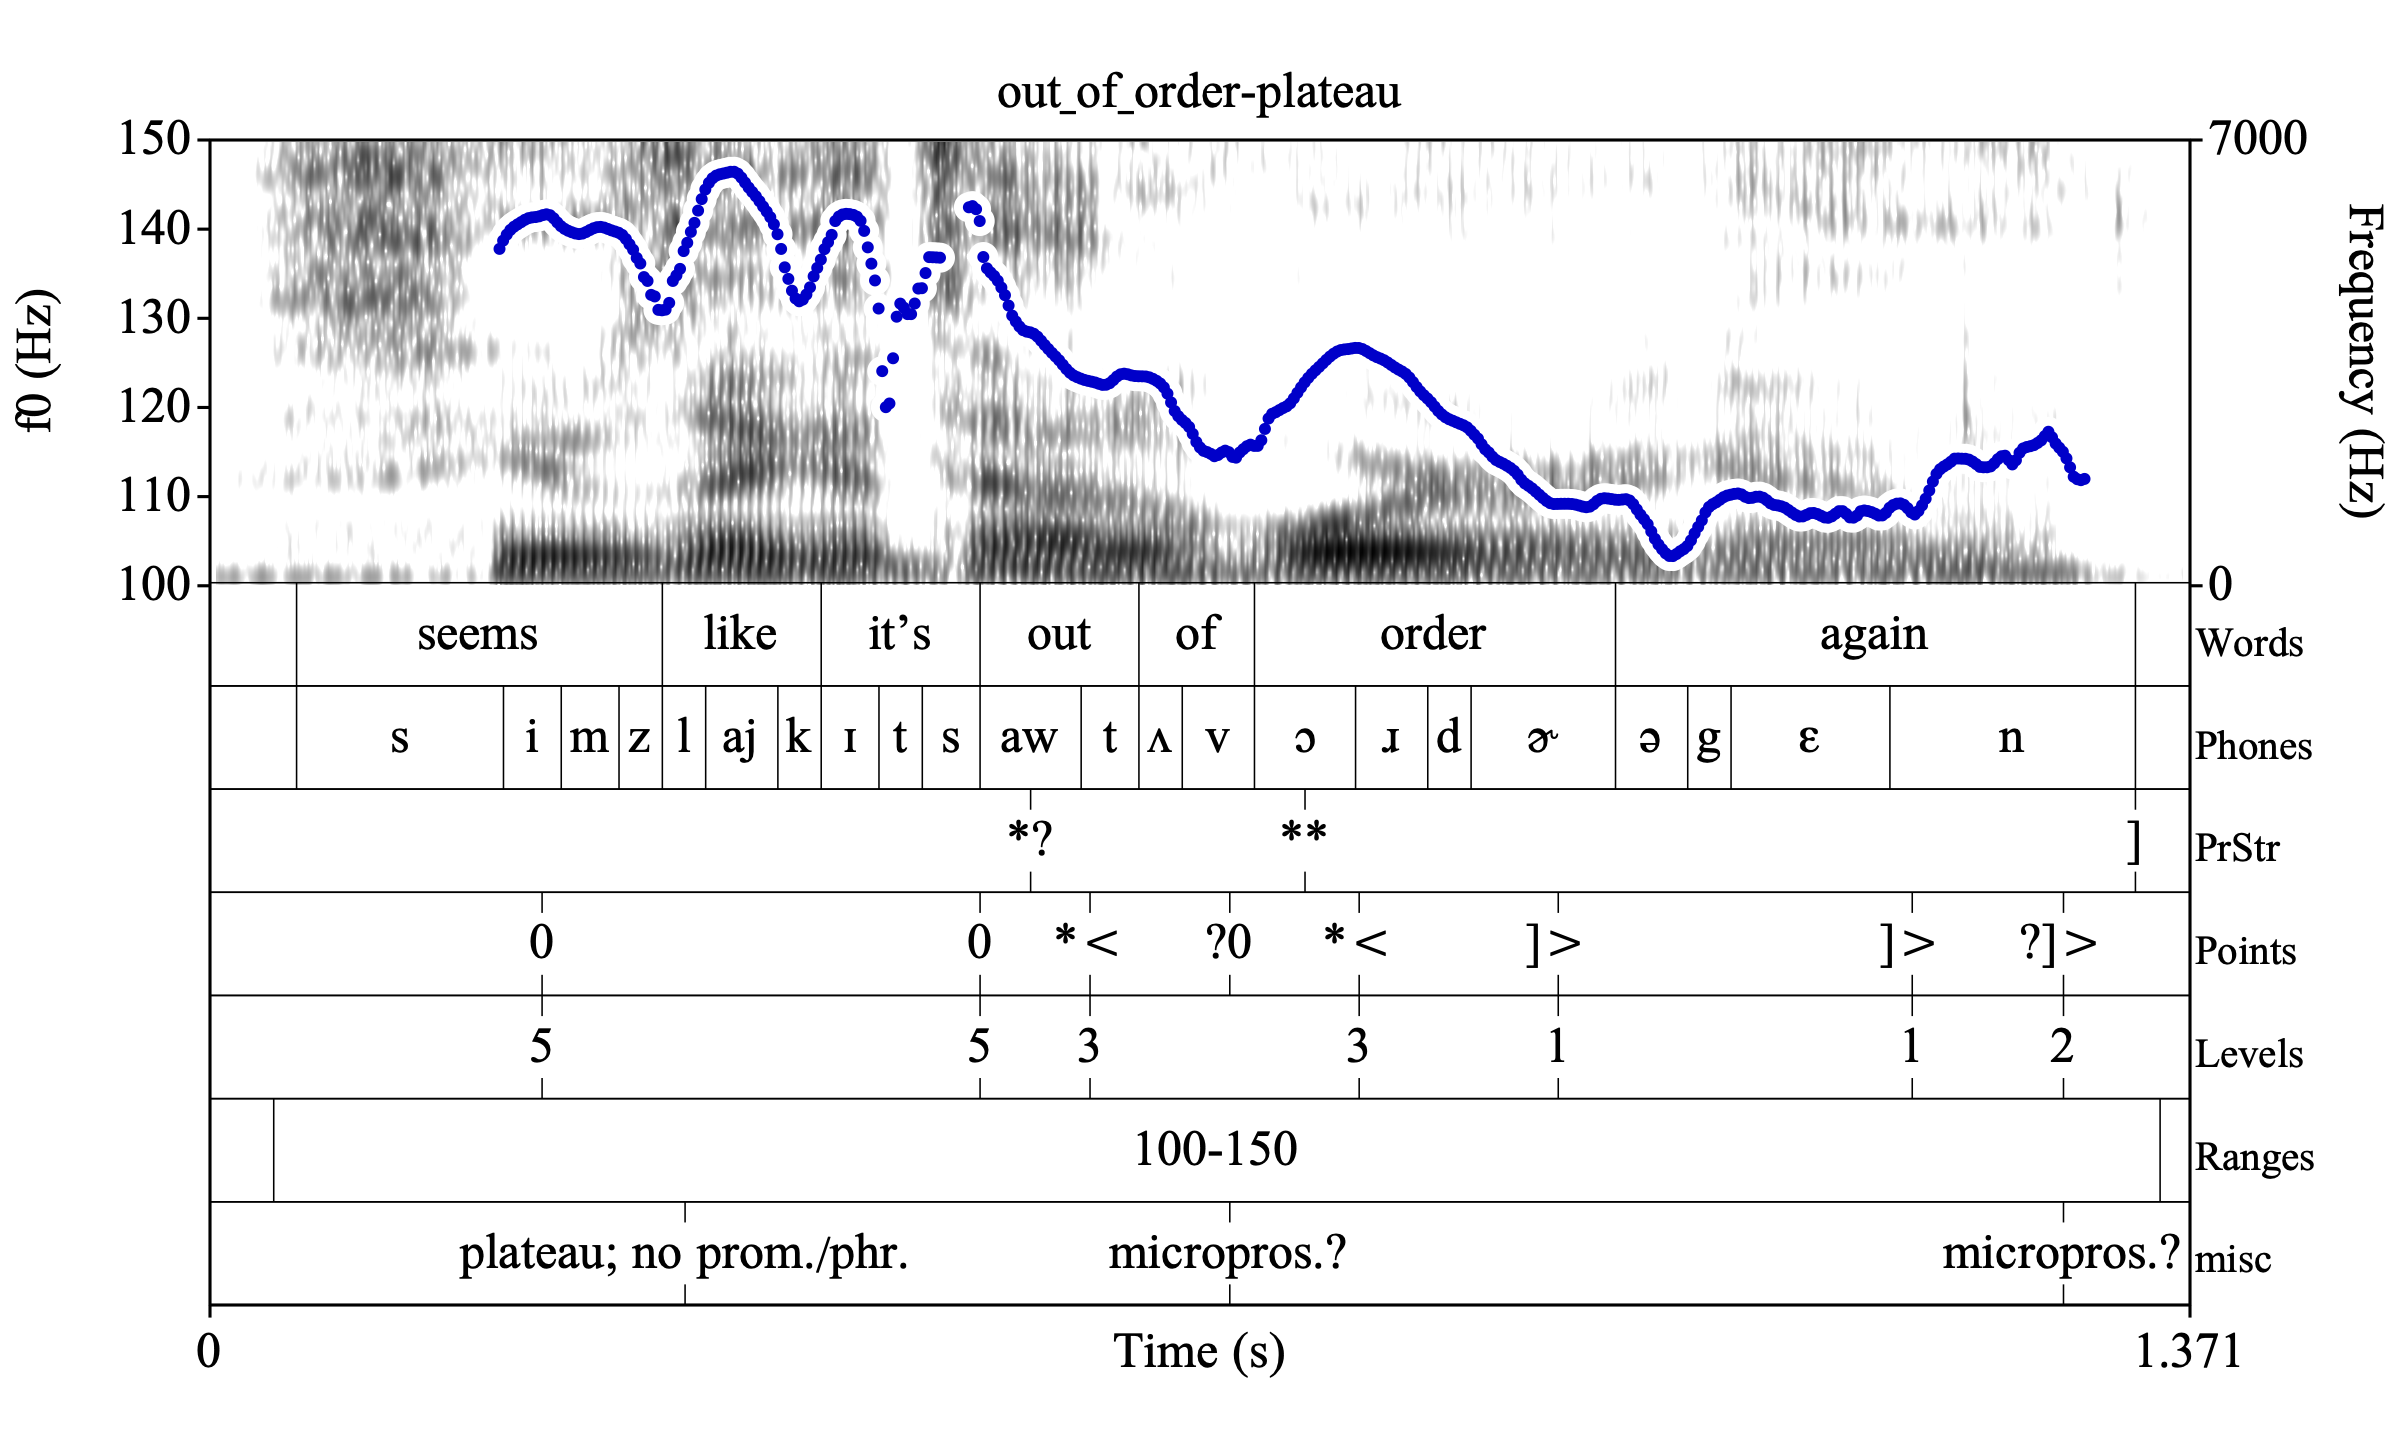
\includegraphics[width=.875\linewidth]{Points-out_of_order-plateau-adv.png}
%
\caption{\texttt{out\_of\_order-plateau}, with Advanced PoLaR labels.%
\label{fig:out_of_order-plateau Points Adv}%
\index{Annotated example, Points tier (advanced)!out\_of\_order-plateau}
}
\end{figure}

We have already discussed the plateau at the beginning of this utterance, in Chapter \ref{ch:basics}. Given the labellers’ lack of phonological analysis for the plateau, these labels remain as ‘\textlabel{0}’s, even when the label is otherwise using the wider array of Advanced Points labels.

This example also has two notable movements in the f0-tracking where the labeller is uncertain. The first is the dip in the tracking between “\langtext{out}” and “\langtext{order}”, and the other is the rise in the tracking at the end of “\langtext{again}”. In both cases, the labeller has begun their Points tier labels with a ‘\textlabel{?}’ to indicate their uncertainty about whether there is a turning point. (One factor contributing to the uncertainty is likely that this utterance is produced in a very narrow pitch range: 100-150Hz, making it hard to ascertain whether a small f0 movement is significant enough to merit a Points label or whether it may be a microprosodic effect, as in the case of the dip during “of” that might be related to the [v].)

\subsection{Summary of the Advanced Labels for the Points Tier}\label{sec:summary-of-the-points-tier}

The PoLaR annotation system, which is neither purely phonetic nor purely phonological, provides a means to make explicit how labelling of acoustic cues is phonologically informed. Moreover, PoLaR is flexible enough that it does not require its labellers to ascribe to any particular phonological model. (Even the set of labels in the Prosodic Structure Tier could be modified to fit different phonological models.) This allows the labeller to not only annotate phonological objects (in the Prosodic Structure tier) and phonetic cues (e.g., f0 turning points), but \uline{also to indicate a mapping relationship}, all without requiring commitment to a particular phonological model (to avoid being an impediment towards wide adoption).

The table below lists 7 Points Tier objects that a PoLaR labeller can use. It is possible to add a ‘\textlabel{?}’ before each label, to indicate labeller uncertainty about the presence of a pitch turning point, and it is also possible to include a numeric value after each label, to indicate labeller intuition about the pitch value (in Hz).

\begin{longtable}{c>{\centering}p{.33\linewidth}>{\centering\arraybackslash}p{.45\linewidth}} \toprule \textbf{Label} & \textbf{Relevant Prosodic Structure object} & \textbf{Relative to an object on the PrStr tier, this f0 turning point is time-aligned…}\tabularnewline
\midrule \endhead
\rowcolor{green}\textlabel{0} & No phonological analysis given by the labeller & N/A\tabularnewline
\midrule
\textlabel{*>} & & …before the relevant \textlabel{*}\tabularnewline
\textlabel{*<} & Prominence: \textlabel{*}, \textlabel{?*}, or \textlabel{**} & …after the relevant \textlabel{*}\tabularnewline
\textlabel{*@} & & …with the relevant \textlabel{*}\tabularnewline
\midrule
\textlabel{]>} & & …before the relevant \textlabel{]}\tabularnewline
\textlabel{]<} & Phrase boundary: \textlabel{]}, \textlabel{?]}, \textlabel{]]} & …after the relevant \textlabel{]}\tabularnewline
\textlabel{]@} & & …with the relevant \textlabel{]}\tabularnewline
\midrule
\textlabel{[>} & & …before the relevant \textlabel{[}\tabularnewline
\textlabel{[<} & Phrase boundary: \textlabel{[}, \textlabel{?[}, \textlabel{[[} & …after the relevant \textlabel{[}\tabularnewline
\textlabel{[@} & & …with the relevant \textlabel{[}\tabularnewline
\bottomrule
\caption[An expanded set of labels for the Points tier, with several advanced options.]{An expanded set of labels for the Points tier, with several advanced options. The fundamental label ‘\textlabel{0}’ is highlighted, with the remaining labels being for labellers with more experience. Note that, as always, a ‘\textlabel{?}’ can be prepended to any of these labels to indicate labeller uncertainty about whether there is indeed a pitch turning point at this time.}
\end{longtable}


(\textit{Note: an individual ‘\textlabel{]}’ on the PrStr tier is very often associated with multiple ‘\textlabel{]>}’, ‘\textlabel{]<}’, or ‘\textlabel{]@}’ targets. Similarly, this sort of many-to-one relationship is also very common for prominence-type annotations.})

\begin{figure}[H]
\centering
%
  \begin{tikzpicture}[node distance=4em, anchor=west, align=flush center, FLOW/.style={->, very thick}, LABEL/.style={draw, fill=yellow!80, inner sep=.75em}, scale = .625, transform shape]
    \node[draw, text width=6em,anchor=east] (node0) {Is the labeller certain that there should be a Point object here?};
    \node (node1) [right=5em of node0] {};
    \node (node1up) [above=1em of node1] {};
    \node (node1down) [LABEL, below=1em of node1] {\textlabel{?}};
    \node[draw, text width=5.5em, right=5em of node1] (node2) {Assert a relationship to a PrStr object?};
    \node[LABEL, below right=1em and 6em of node2.east] (node3no) {\textlabel{0}};
    \node[LABEL, above right=1em and 6em of node2.east] (node3yes) {\textlabel{*}\\\textlabel{]}\\\textlabel{[}};
    \node[draw, text width=8em, right=3em of node3yes] (node4) {Where is the PrStr Tier object that corresponds to the Points Tier object?};
    \node[LABEL, right=3em of node4.east] (node5) {\textlabel{>}\\\textlabel{<}\\\textlabel{@}};
    \node[draw, text width=8em, below=5.5em of node5, anchor=north] (node6) {Could this Points Tier object also correspond to another PrStr object?};
    \node[right=3em of node6] (node7yes) {};
    \node[LABEL, above=of node7yes.center] (node7) {\textlabel{/}};
    \node[above=9em of node7] (node7-loopback1) {};
    \node[above=2em of node3yes] (node7-loopback2) {};
    \node[draw, text width=10em, below=2em of node3no] (node8) {Does the labeller want to directly annotate a value for the pitch (in Hz) for this Point?};
    \node[LABEL, text width=8em, left=of node8] (node9) {\textlabel{,}<\textit{value in Hz}>};
%%%%%%%%%%%%%%%
%%%%%%%%%%%%%%%
    \draw [black,FLOW] (node0.east) -- node[pos=0.5,below, sloped]{No} (node1down.west);
    \draw [black,FLOW] (node1down.east) -- (node2.west);
    \draw [black,FLOW] (node0.east) -- node[pos=0.5, above, sloped]{Yes} (node2.west);
    \draw [black,FLOW] (node2.east) -- node[pos=0.5, above, sloped]{Yes} (node3yes.west);
    \draw [black,FLOW] (node2.east) -- node[pos=0.5, above, sloped]{No} (node3no.west);
    \draw [black,FLOW] (node3yes.east) -- (node4.west);
    \draw [black,FLOW] (node4.east) -- (node5.west);
    \draw [black,FLOW] (node3no.south) -- (node8.north);
    \draw [black,FLOW] (node5.south) -- (node6.north);
    \draw [black,FLOW] (node6.west) -- node[pos=0.5, above, sloped]{No} (node8.east);
    \draw [black,FLOW] (node6.east) -- node[pos=0.5, above, sloped]{Yes} (node7yes.center) -- (node7.south);
    \draw [black,FLOW] (node7.north) --  (node7-loopback1.center) -- (node7-loopback2.center) -- (node3yes);
    \draw [black,FLOW] (node8.west) -- node[pos=0.5, above, sloped]{Yes} (node9.east);
  \end{tikzpicture}
%
\caption{A finite state grammar for Advanced Points tier labels.%
\label{fig:Points FSG complete}%
\index{Grammar (finite state), Advanced Points labels}
}
\end{figure}


\section{Ranges (Advanced)}\label{sec:ranges-advanced}

As described in Chapter \ref{ch:basics}, the Ranges tier defines the pitch space in which the Points tier labels are to be interpreted via the Levels tier, giving it a critical role in describing local pitch dependencies, such as within a prosodic phrase. But a range is not always limited to a single phrase; a further advantage of annotating ranges is the ability to annotate more complicated pitch relations across longer stretches of speech, allowing labellers to capture observed\slash intuited cross-phrase relations. By delinking the designation of pitch ranges from phrasing, PoLaR can shed light on the complex ways in which tonal cues interact with other cues to prosodic grouping and prominence. In this section, we discuss in detail some ways in which the Ranges tier labels can reflect labeller intuitions about relations among local ranges, as well as interactions across PoLaR tier labels. We will look at common types of range changes that occur within even a short utterance, as well as how ranges may interact across longer stretches of speech.

The idea of variable local pitch ranges within an utterance may be familiar to those labellers who have experience with other labelling frameworks, such as ToBI, in which it is generally understood that a local pitch range can change in the middle of the utterance. For example, the ToBI guidelines indicate that, even within a single utterance, “[e]ach new intermediate phrase represents a new paradigmatic choice of pitch range” (\citealt{beckmanayers97}:p.25). A familiar example is the highly compressed pitch range often used for a parenthetical (see, e.g., \citealt{dehewichmann10}; we discuss parentheticals and cases similar to them in later sections of this chapter.

Even though there may be a connection between local pitch ranges and particular sorts of prosodic phrases, as made explicit in phonological models of intonation (as with ToBI; but see section \ref{sec:how-tobi-and-polar-treat-ranges}, which contrasts PoLaR and ToBI treatments of ranges), PoLaR does not require the labeller to always attend to any particular definition of (syntactic\slash prosodic) phrase boundaries when making decisions about pitch range intervals. (i.e., A labeller need not (i) have a particular definition of constituents like “intermediate phrase”, (ii) be able to recognize constituents on the basis of phonetic cues, or (iii) have a theory of the alignment between constituent structure and pitch range changes.) Instead of relying on an existing linguistic theory that would predict where range changes will occur, the primary direction for labelling pitch range is that the labeller should rely on their intuition as to which regions of an utterance belong to separate pitch range intervals. (In the last part of this section, we will return to the idea of intuition, and what sorts of things a labeller may wish to attend to in sorting out their intuitions.)

Because the ranges are labelled separately from prosodic phrasing, local pitch range intervals are not constrained by the boundaries. (This even allows Ranges and PrStr to be annotated separately, perhaps even by separate labellers.) Just as we saw that a pitch range could span more than a phrase (in the example, \texttt{tomorrow\_morning}, in Figure \ref{fig:tomorrow_morning Ranges basic} of Chapter \ref{ch:basics}), we can also have ranges that begin\slash end in the middle of a prosodic phrase (as delineated by boundaries annotated on the PrStr tier). In other words, a single prosodic phrase may contain multiple Ranges intervals.

\subsection{A complex example of many range changes}\label{sec:a-complex-example-of-many-range-changes}

Let us begin by imagining a set of utterances with a complex set of changes in ranges. A particular individual may have a physiological pitch range of 50-700 Hz, while their comfortable implementable pitch range may be 60-425Hz. As we have already discussed, the local pitch ranges will typically be smaller than either of these ranges, and may occur across various stretches of pitch space at various points during speech. Below is an idealization of four hypothetical utterances (in different colors) produced by a single speaker; note that some of these utterances are themselves composed of multiple local pitch ranges:

\begin{figure}[H]
\centering
%
\begin{tikzpicture}
\draw (0,4.5) -- (0,0) -- (9,0);
\node[rotate=90] at (-1,2.25) {\relsize{-.5}f0 (Hz)};
\begin{scope}[anchor=east, style={font=\relsize{-1}\bfseries}]
	\node at (0,0) {0};
	\node at (0,1) {100};
	\node at (0,2) {200};
	\node at (0,3) {300};
	\node at (0,4) {400};
\end{scope}
\begin{scope}[anchor=north,align=center, style={font=\relsize{-1}\bfseries}]
	\node at (1,0) {Utt.1\\pt.1};
	\node at (2,0) {Utt.1\\pt.2};
	\node at (3,0) {Utt.2\\pt.1};
	\node at (4,0) {Utt.2\\pt.2};
	\node at (5,0) {Utt.3\\pt.1};
	\node at (6,0) {Utt.3\\pt.2};
	\node at (7,0) {Utt.3\\pt.3};
	\node at (8,0) {Utt.4};
\end{scope}
\draw[fill=CB1] (.8,.75) rectangle (1.2,3.6);
\draw[fill=CB1] (1.8,.75) rectangle (2.2,1.6);
%
\draw[fill=CB2] (2.8,1) rectangle (3.2,2.25);
\draw[fill=CB2] (3.8,2.5) rectangle (4.2,3.45);
%
\draw[fill=CB3] (4.8,1) rectangle (5.2,2.2);
\draw[fill=CB3] (5.8,1) rectangle (6.2,4.1);
\draw[fill=CB3] (6.8,.5) rectangle (7.2,2);
%
\draw[fill=CB4] (7.8,.5) rectangle (8.2,1.25);
\end{tikzpicture}
%
\caption[An idealization of pitch ranges in four hypothetical utterances.]{The y-axis is f0 (in Hz) and each of the bars indicates the speaker’s local pitch range in particular (hypothetical) utterances; successive utterances are indicated by color changes.%
\label{fig:Ranges bars}%
%\index{Annotated example, Ranges tier (advanced)!XXXXX}
}
\end{figure}


To reiterate, the Ranges that are annotated as intervals on the tier are intended to indicate what the labeller believes would constitute a “high” pitch in this local interval of time, and what would constitute a “low” pitch in the same interval. In this way, what the labeller is doing is making some postulations about how they believe the speaker is setting their pitch range during a particular time interval. An example that mirrors the idealization in Figure \ref{fig:Ranges bars} is provided, in Figure \ref{fig:long-story-ranges Ranges Adv}.

\begin{figure}[H]
\centering
%
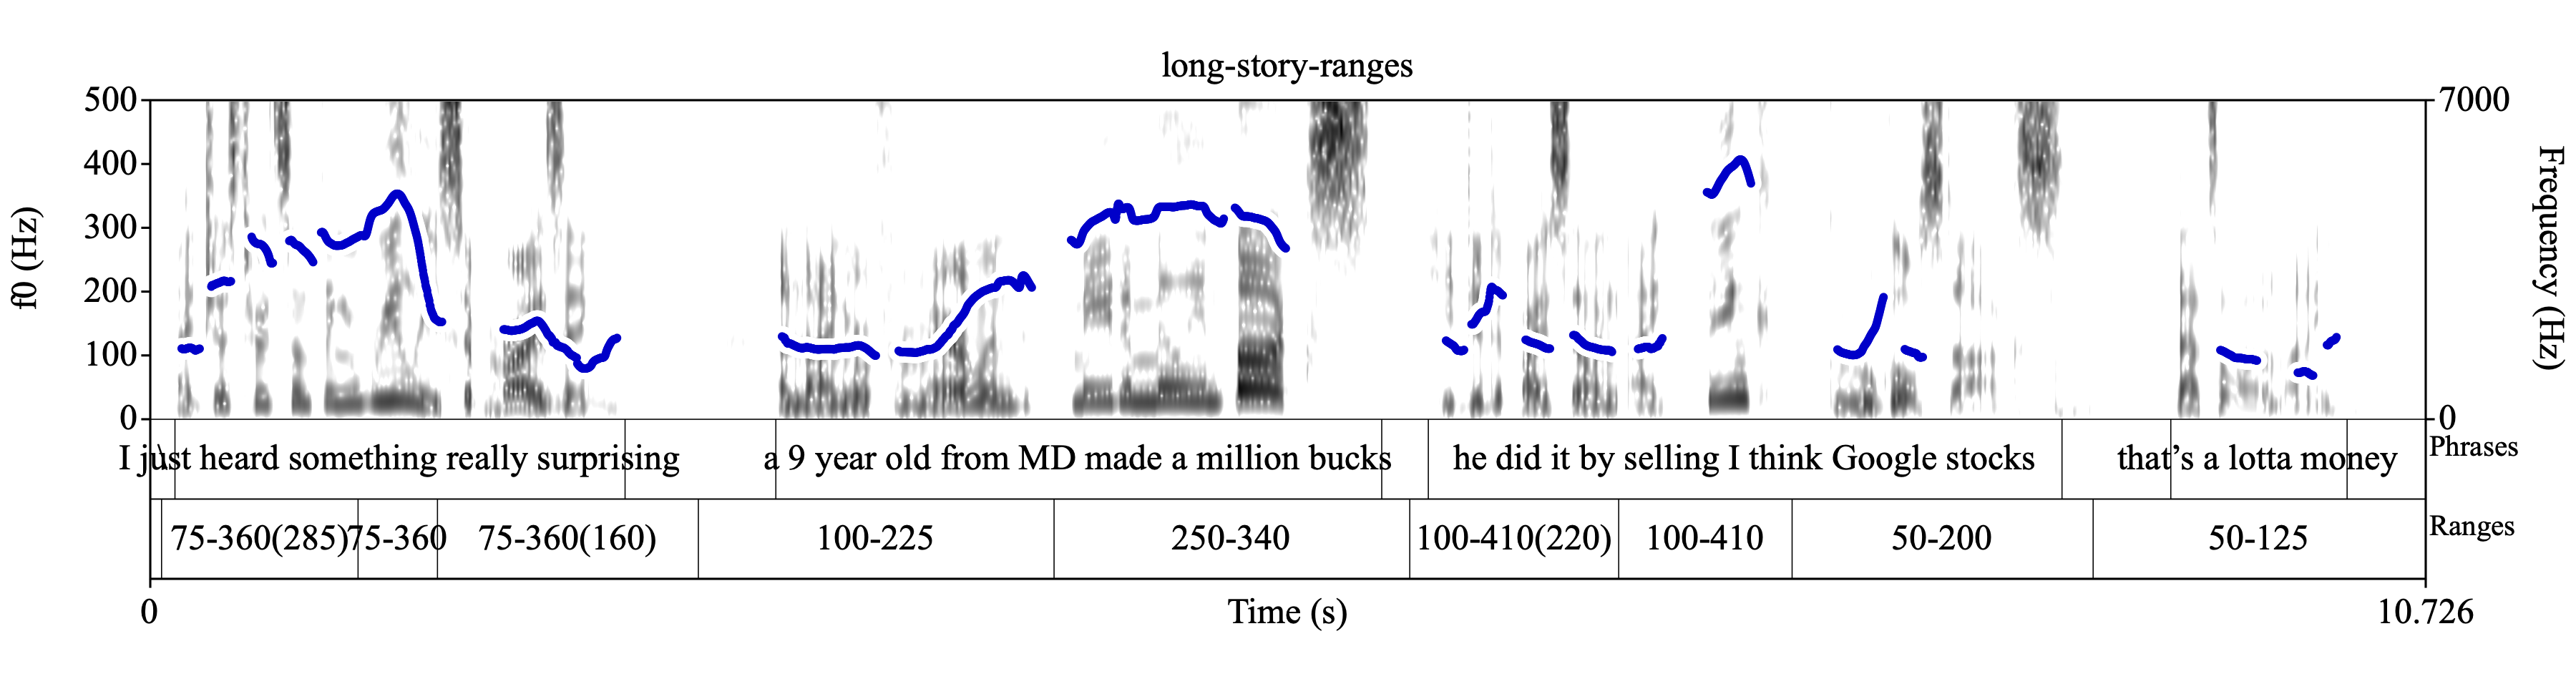
\includegraphics[width=\linewidth]{Ranges-long-story-ranges-adv.png}
%
\caption[An example of four utterances with nine pitch range intervals.]{An example of four utterances with nine pitch range intervals. Note that words are not aligned with the speech signal or the Range constituent intervals.%
\label{fig:long-story-ranges Ranges Adv}%
\index{Annotated example, Ranges tier (advanced)!long-story-ranges}
}
\end{figure}

Consider the interval following the first pause (\langtext{a 9 year\ldots}), labelled ‘\textlabel{100-225}’, and compare that to the following interval (\langtext{made a\ldots}) labelled ‘\textlabel{250-340}’. The specific annotation indicates that the labeller perceives that a pitch of 225 Hz on \langtext{Maryland} would certainly count as a “high” (and would be transcribed with a value of ‘\textlabel{5}’ on the Levels tier) in the first part of this utterance. However, moments later (during \langtext{made a…}), 250Hz is perceived as the “low” floor of this interval (and would be transcribed with a value of ‘\textlabel{1}’ on the Levels tier).

In particular, the relevant aspect of intuition concerns “what goes together” as a pitch range constituent. To make this clear, let’s zoom in on \langtext{he did it by selling I think Google stocks} in the previous example and discuss why the labeller has labelled \langtext{I think} as a pitch range (sub)interval, rather than including \langtext{I} as part of the preceding pitch range interval, despite the fact that it begins with a low f0 very close to the f0 of the preceding word.

\begin{figure}[H]
\centering
%
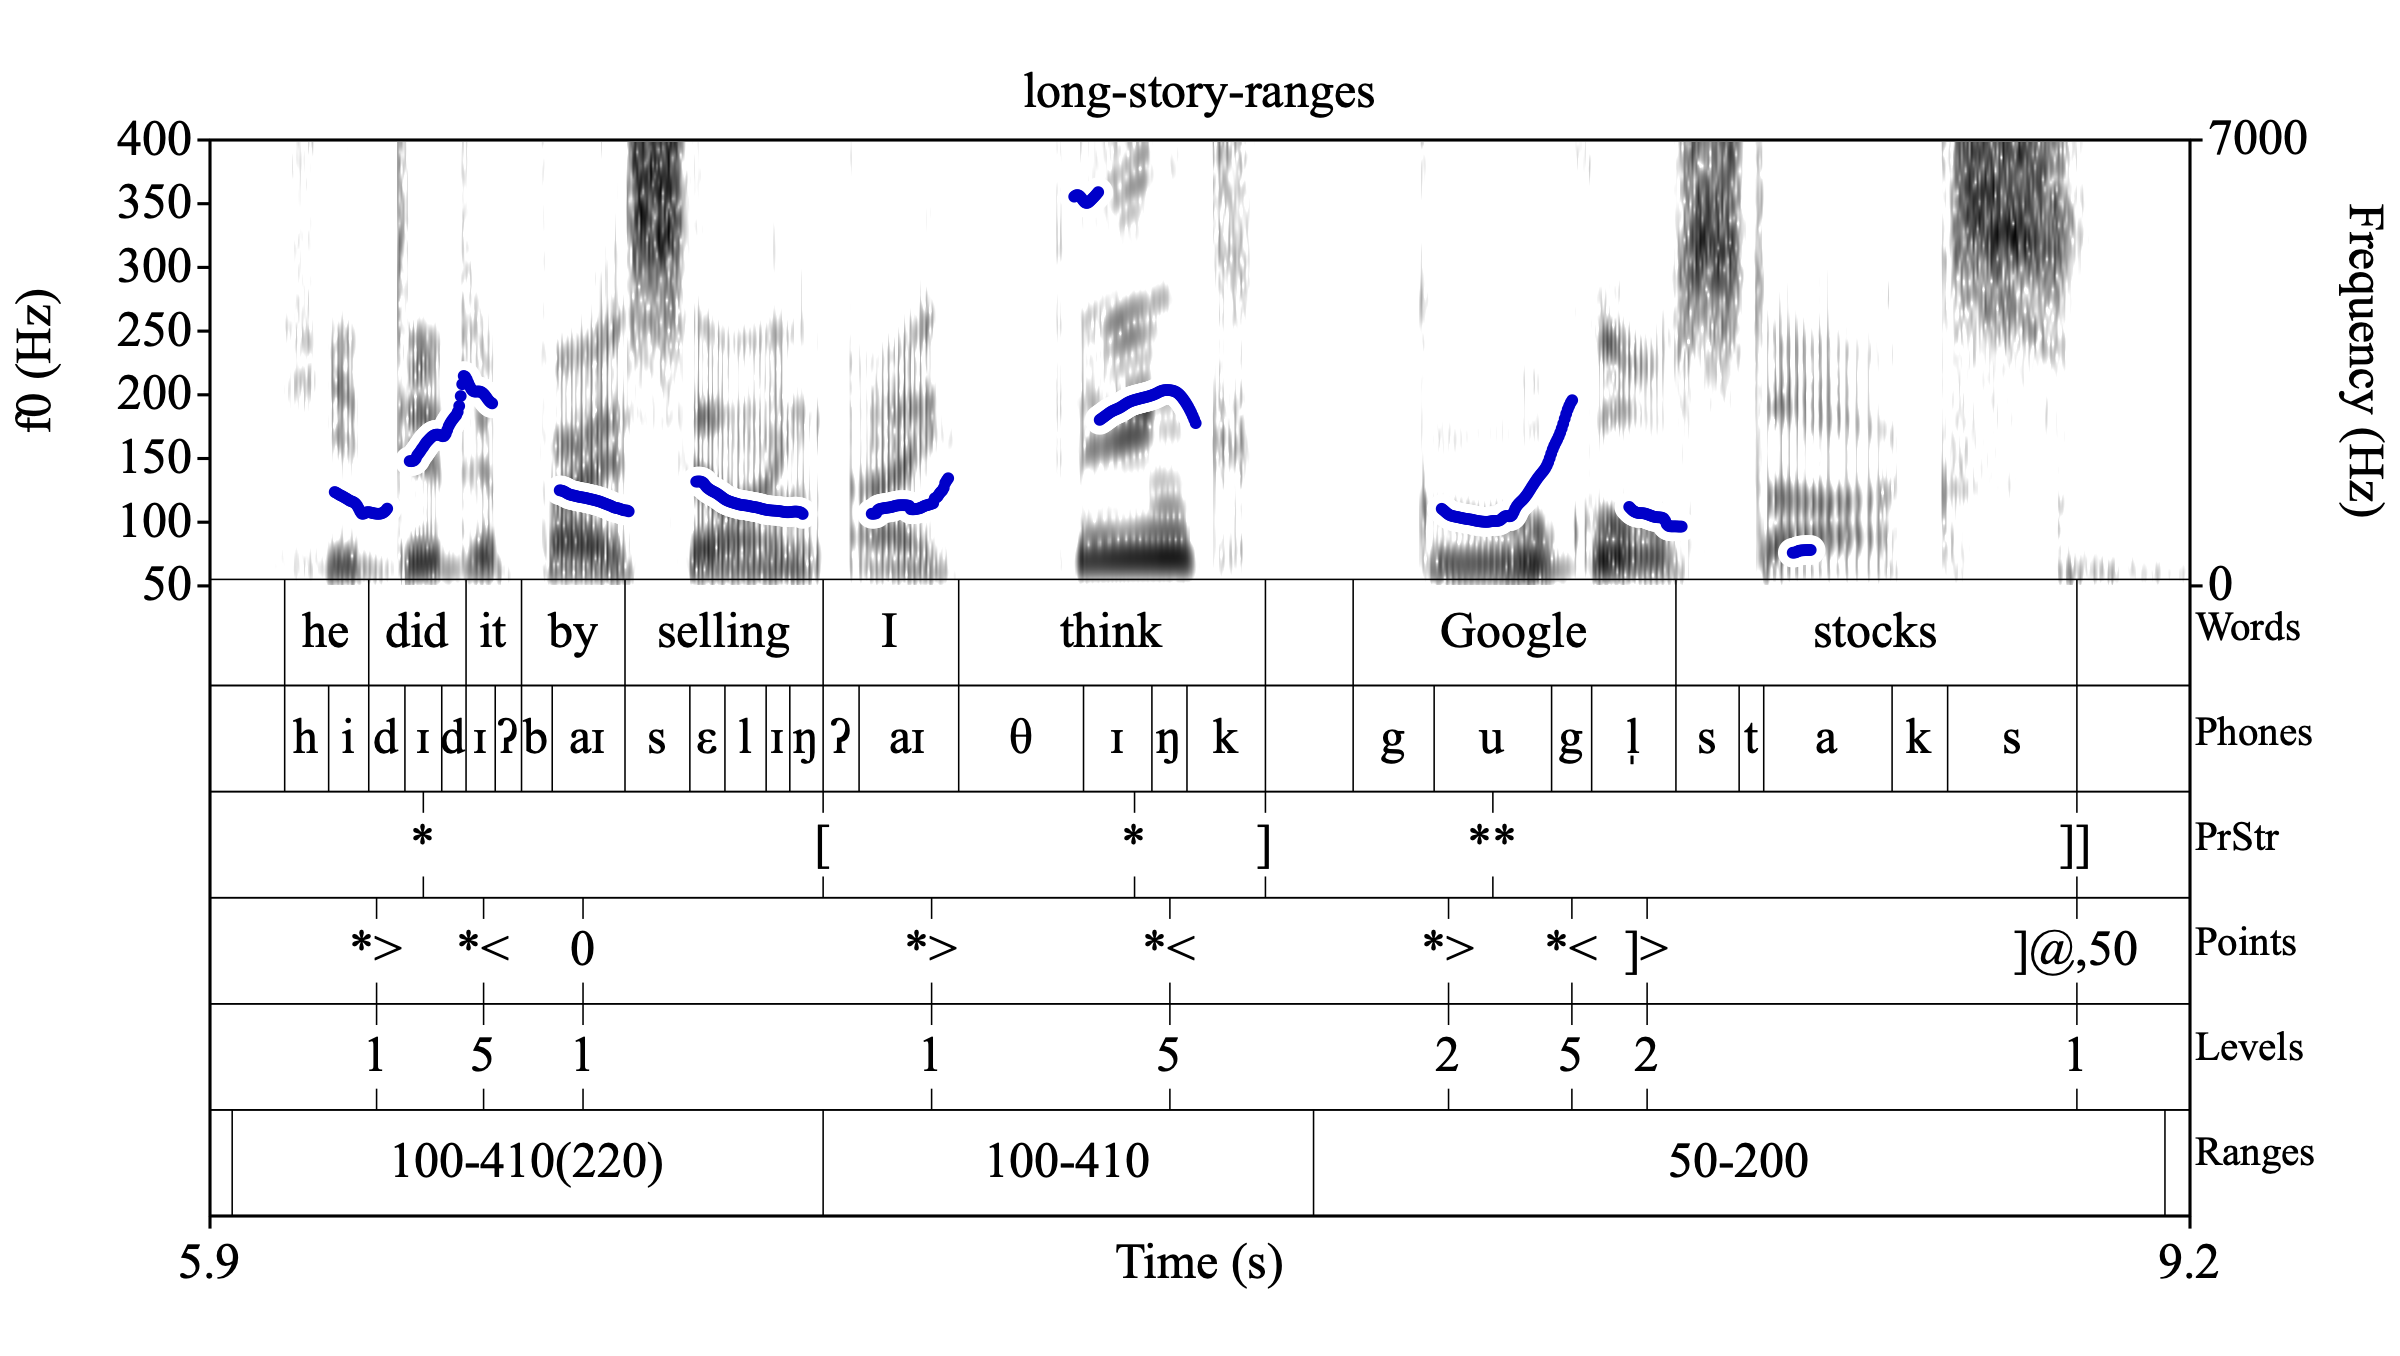
\includegraphics[width=.875\linewidth]{Ranges-long-story-ranges-adv-short.png}
%
\caption{A closer look at some Ranges intervals.%
\label{fig:long-story-ranges short Ranges Adv}%
\index{Annotated example, Ranges tier (advanced)!long-story-ranges}
}
\end{figure}

In this figure, we can see that the three pitch range constituents map onto the following strings of words: \langtext{he did it by selling}, \langtext{I think}, and \langtext{Google stocks}. Looking at this pitch track alone, it isn’t obvious that \langtext{I} should be part of the same pitch range constituent as \langtext{think} – that is, one might wonder whether \langtext{think} should constitute a complete pitch range constituent in itself, such that \langtext{I} is part of the preceding one. There are a few reasons why the labellers in this case have grouped \langtext{I think} together, all of which are strongly linked to their intuitions as English speakers. First and foremost: it is clear that the f0 during \langtext{think} is very high, in a different local range than the “high” pitches in surrounding words; while it is therefore clear (solely on the basis of measurements) that the local pitch maximum is around 410Hz, determining a value for the local pitch minimum requires consulting some intuitions about how words are grouped together and/or analyzing some additional cues to grouping in the signal. What are the relevant sources of information that underlie these (tacit) intuitions and (conscious) analyses? The answer lies in constituency (of various types), and the cues to constituency.

Let’s step back and look at the basic ideas behind local pitch ranges. We assume that local pitch ranges (which is what the Ranges tier aims to annotate) map onto constituents of some type(s), even if we are not entirely certain yet what those are. Language encodes various types of constituency, whose boundaries determine various linguistic properties: (i) ability to be manipulated syntactically, (ii) domains of semantic interpretation, and (iii) senses of juncture in speech informed by (for example) the beginnings\slash ends of coherent pitch contours, the local pitch range, placements of silence, final lengthening, and initial strengthening, among many other properties.\footnote{Not every boundary corresponds to all of these factors named above, and these cues can also be used to signal different aspects of structure (such as lengthening associated with prominence). Moreover, different types of constituents may be signalled by different types of cues. (It may even be that there are constituents which are only detectable through one of these properties, instead of a constellation of them.)} In this way, finding the beginning\slash end of a pitch range interval can be aided by finding other cues to the beginning\slash end of a constituent (with respect to any one of these linguistic properties; or more likely, with respect to multiple coinciding properties).

Returning to the example, let us review three reasons why one might want to label the Range interval constituent as the word sequence \langtext{I think} (and, e.g., not just the single word \langtext{think}). Let’s start with an f0-based intuition about constituency. When the annotators labelled this, they intuited that there is a single pitch movement —a large rise from low to high— which includes the pitch values during \langtext{I}. That is, the relevant pitch movement does not occur solely within the word \langtext{think} (where there is a rise from around 325Hz to 410Hz); instead, it is intuited as a rise from within \langtext{I} to within \langtext{think} (a rise of about 105Hz to 410Hz). It may be that if this interval consisted of continuous sonorant material, e.g. \langtext{I wink}, we would see more clear pitch-based evidence that there is a single f0 ‘scoop’ that starts in \langtext{I}. A second way in which prosody may contribute to the intuition of constituency might be based in the fact that there is a brief period of glottal closure between \langtext{selling} and \langtext{I}, resulting in a brief silence and initial strengthening in the form of a glottal release at the onset of \langtext{I}. Since glottal marking of this kind is common in American English (see \citealt{dilley-96}), its presence here may contribute to the intuition that a new constituent begins at the onset of \langtext{I}. Third and finally, “\langtext{I think}” maps on to a syntactic\slash semantic constituent (the evidence for which we won’t discuss here). If we kept the f0 the same, but changed the words from \langtext{…selling I think…} to \langtext{…selling it but…} (where the extra high pitch falls entirely on \langtext{but}), there might be some cause to shift the Ranges interval to encapsulate only \langtext{but} – \langtext{it but} is not a syntactic\slash semantic constituent. (Of course, one would also need to weigh these factors against other cues, such as the placement of glottal events.)

To summarize the previous three paragraphs, there are three locally defined pitch ranges labelled above, and they may or may not map onto the boundaries of any currently-well-defined type of prosodic phrase (e.g., the ToBI intermediate phrase). In this way, instead of being forced to attend to predefined sets of cues, labellers are encouraged to attend to their intuitions (which are underwritten by a network of cues, not all of which are always present). In other words, the labeller should not feel restricted by particular perceptions about where (syntactic or prosodic) boundaries are.

\subsection{How Many Range Intervals? Different Approaches and Their Implications}\label{sec:how-many-range-intervals-different-approaches-and-their-implications}

Whereas complete PoLaR labels must have at least one range annotated for every utterance, it will often be the case that an utterance has more than one range. A beginning labeller might start off by labelling ranges relatively sparsely, such as choosing a range for each interval of speech separated by noticeable silent intervals. As labellers become more comfortable with labelling, they may develop more detailed intuitions about local range changes, and therefore label more (and shorter) range domains for the same utterance that was annotated with a single range by a beginner labeller. That is to say, a more advanced labeller is likely to label \uline{more range changes} than a beginner labeller.

One important goal of fine-grained labelling of ranges is that it allows for salient pitch changes from low to high to be captured using Levels annotations, even if those pitch ranges may be smaller than nearby range changes. (i.e., A fall that is perceived as going from high to low might involve a drop in pitch by 200Hz in one part of an utterance, where it may only involve a change of 50 Hz in another part.)

The recording in \texttt{out\_of\_order-ranges} exemplifies this issue well; in particular, both “\langtext{seems}” and “\langtext{order}” both sound high.  In this passage, we will consider different ways of labelling the Ranges tier for this utterance. In Figure \ref{fig:out_of_order-ranges 1range Ranges Adv}, the single phrase (note the lack of phrasing labels on the PrStr tier) has been labelled with a single Range interval (‘150-400’).

\begin{figure}[H]
\centering
%
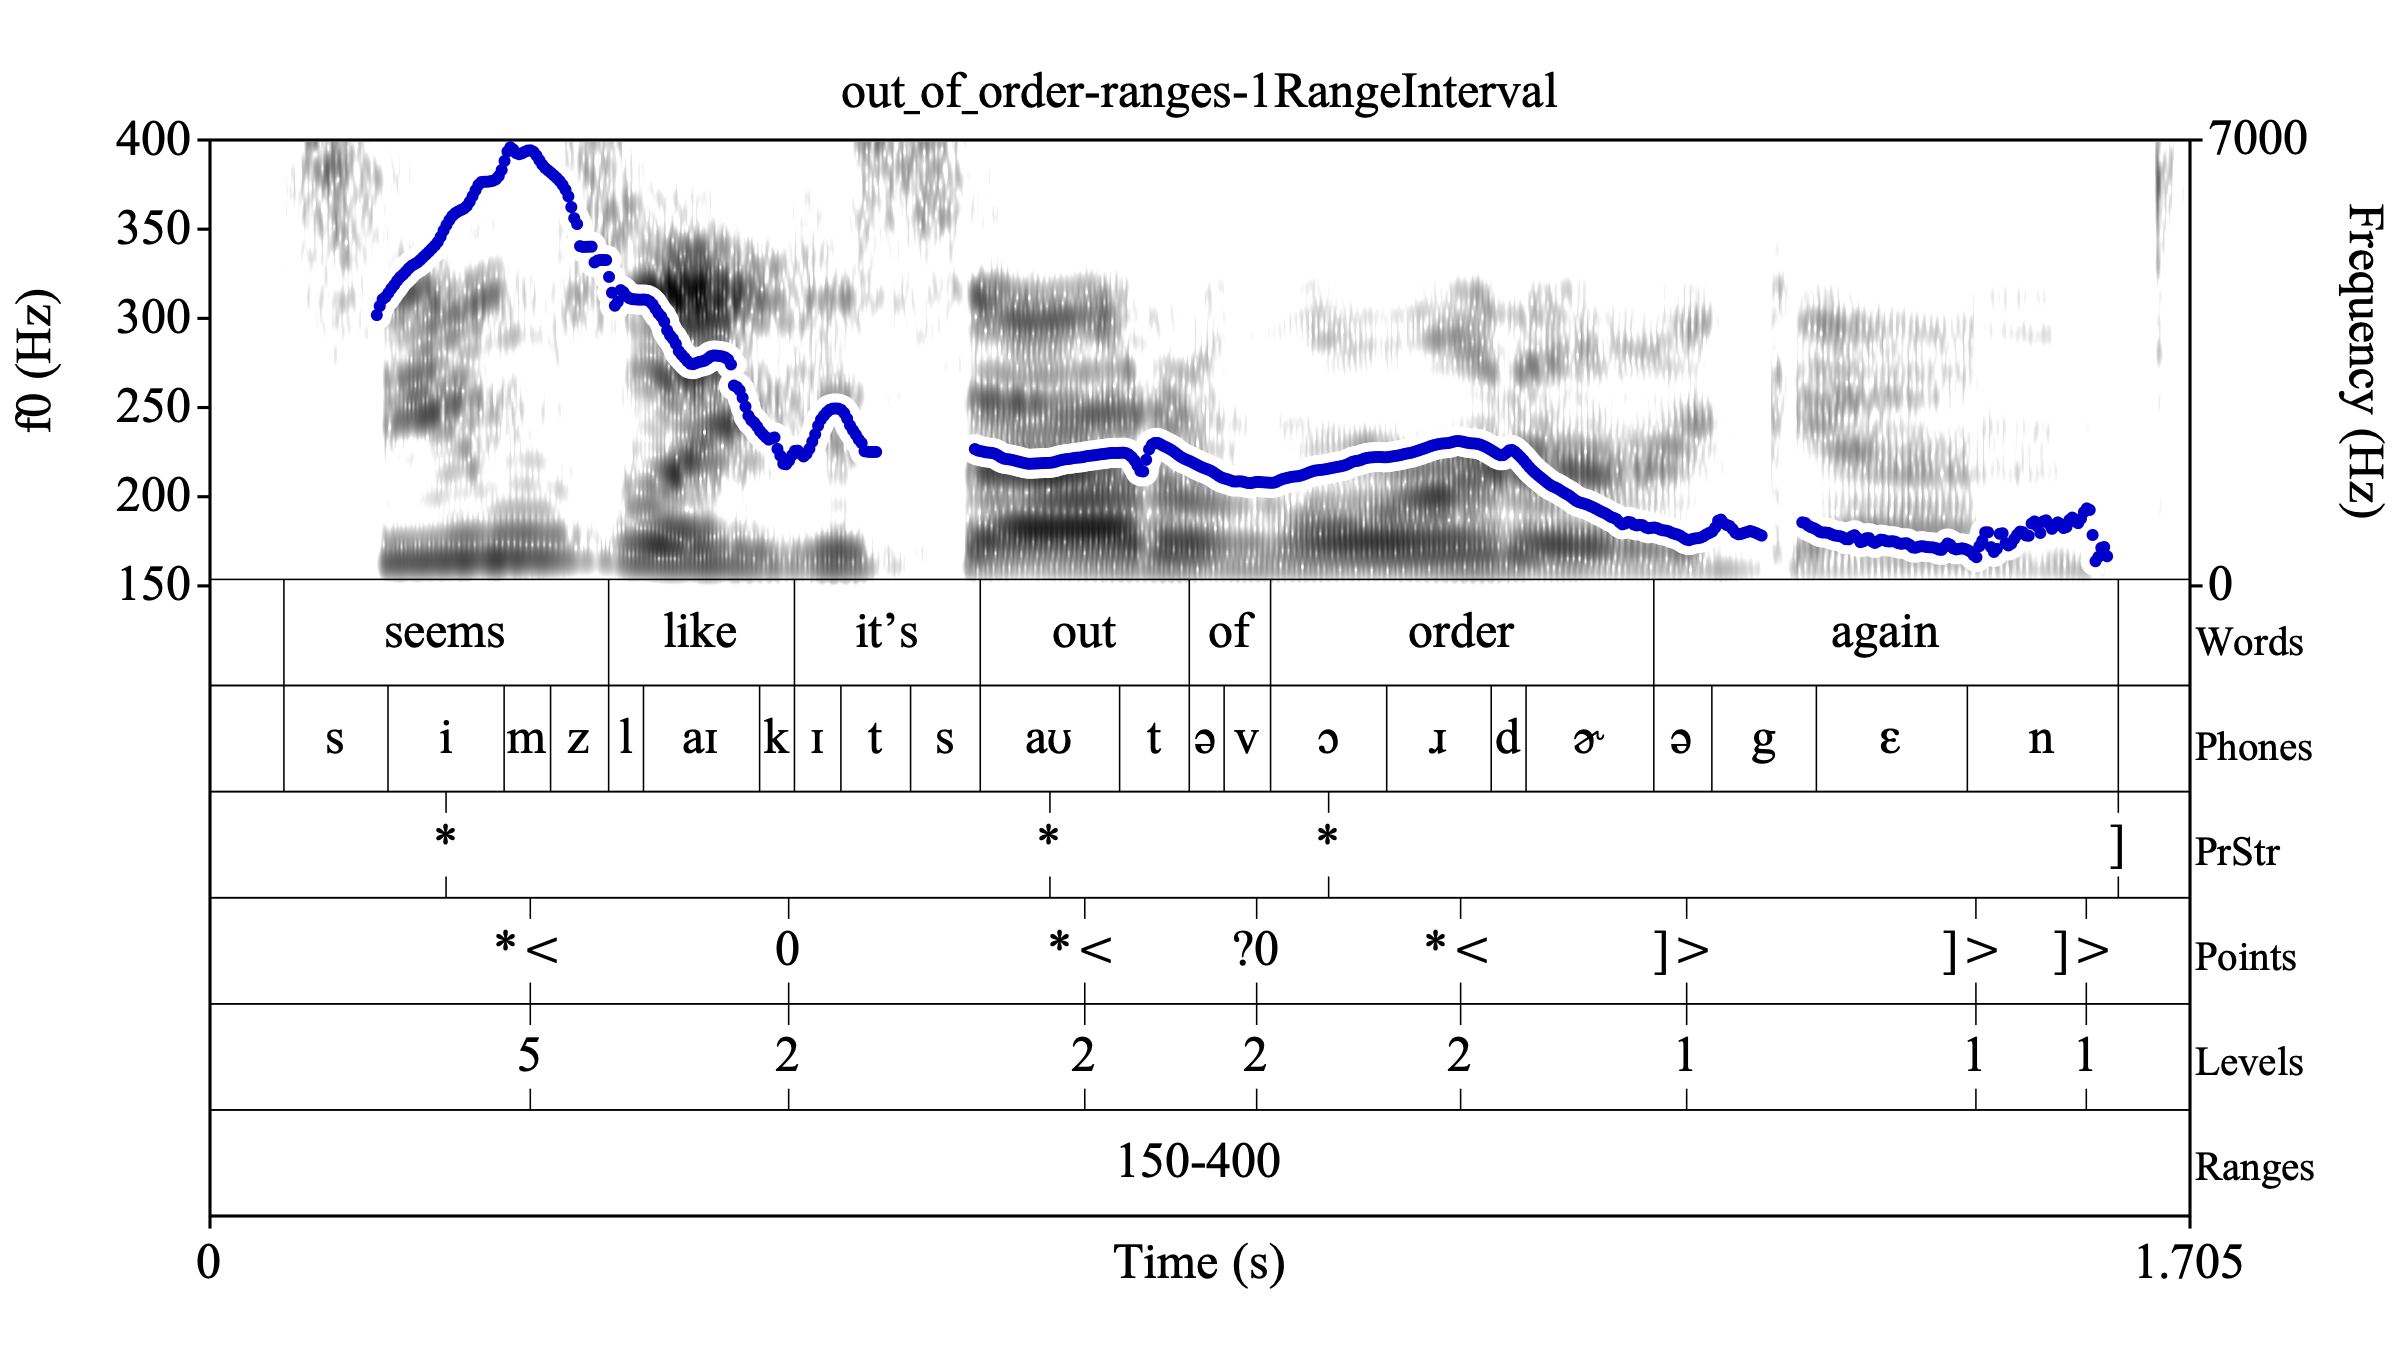
\includegraphics[width=.875\linewidth]{Ranges-out_of_order-ranges-1RangeInterval.png}
%
\caption[A single Range interval for the entire utterance.]{The recording in \texttt{out\_of\_order-ranges} labelled with a single Range interval for the entire utterance.%
\label{fig:out_of_order-ranges 1range Ranges Adv}%
\index{Annotated example, Ranges tier (advanced)!out\_of\_order-ranges}
}
\end{figure}

Whereas this approach to Ranges labelling is not wrong, per se, it does not capture many labellers’ intuitions about the pitch contour in the second half of the recording. Namely, labelling only one long Range interval misses the intuition that “\langtext{order}” is perceived as high in the speaker’s \emph{local range}. (Note that this type of pitch shift downward, i.e. a local compression of the range which includes what is commonly known as downstep, will be discussed in more detail in the next section.)

In addition, some small but still salient pitch movements are not reflected in the Levels, because of the (Basic) single range annotated in the Ranges tier. Listeners report hearing a pitch rise in the first syllable of “\langtext{order}”, but both Levels labels in this syllable have the same value of 2. This is because Levels directly follow Ranges labels, as illustrated in Figure \ref{fig:out_of_order-ranges rainbow Ranges Adv}, by way of the horizontal bands representing the pitch quintiles encoded as Levels labels.

\begin{figure}[H]
\centering
%
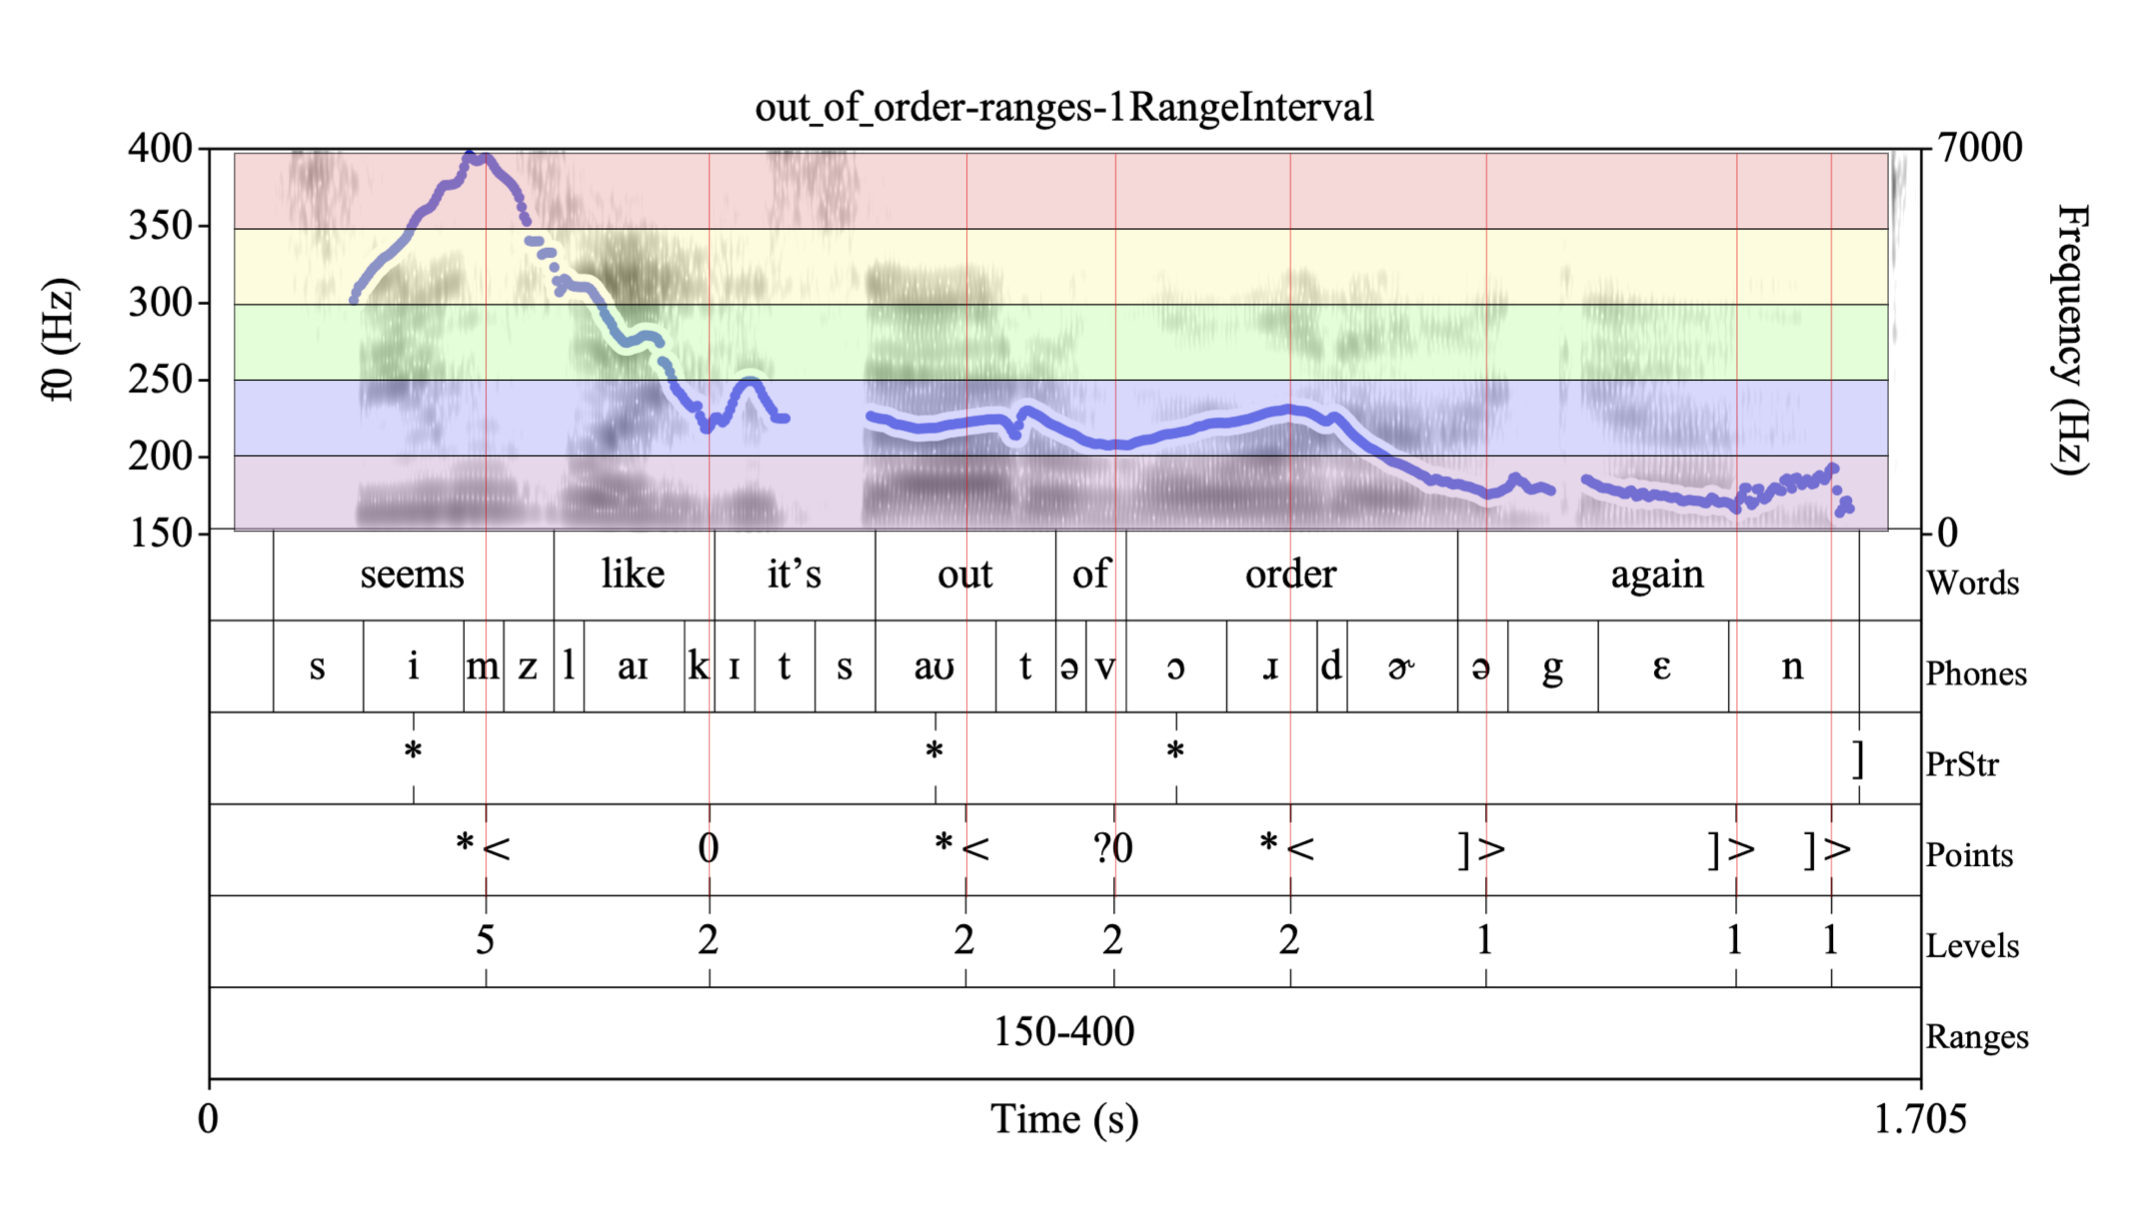
\includegraphics[width=.875\linewidth]{out_of_order-ranges-1RangeInterval-rainbow.png}
%
\caption[Each colored band represents the chunk of pitch space corresponding to each numbered Level, 1-5.]{Each colored band represents the chunk of pitch space corresponding to each numbered Level, 1-5, as determined by the min and max values labelled in the sole Ranges interval.%
\label{fig:out_of_order-ranges rainbow Ranges Adv}%
\index{Annotated example, Ranges tier (advanced)!out\_of\_order-ranges}
}
\end{figure}

In other words, a single Ranges interval here does not capture the intuition of a significant pitch rise during “\langtext{or-}”, since that Ranges interval places both Levels labels in the same pitch quintile.

By contrast, to account for listeners who hear a rise in pitch during order, the Ranges tiers can be labelled as in Figure \ref{fig:out_of_order-ranges rainbow Ranges Adv}. The beginning of the utterance is given a range of 150-400Hz, but the second range has a compressed range of 150-230Hz, encoding a local rise in pitch.\footnote{Note that the first Ranges interval has a pitch floor of 150Hz, which is not attested in this portion of the utterance. We clarify why one might want this to be 150Hz in discussions of pitch floors (section \ref{sec:ranges-and-pitch-floors}) and Levels (section \ref{sec:the-influence-of-levels-and-ranges-on-one-another}).}

\begin{figure}[H]
\centering
%
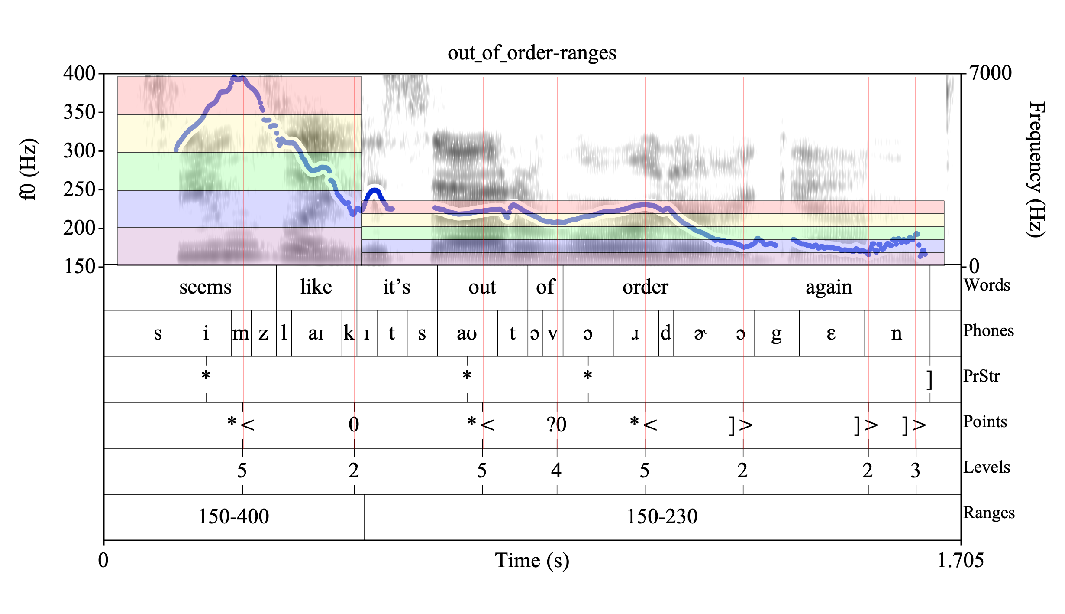
\includegraphics[width=.875\linewidth]{out_of_order-ranges-2RangeIntervals-noparens-rainbow.pdf}
%
\caption[Each colored band represents the chunk of pitch space corresponding to each numbered Level, 1-5.]{Each colored band represents the chunk of pitch space corresponding to each numbered Level, 1-5, as determined by the min and max values labelled in each of the two Ranges intervals.%
\label{fig:out_of_order-ranges 2range no() Ranges Adv}%
\index{Annotated example, Ranges tier (advanced)!out\_of\_order-ranges}
}
\end{figure}

The second Ranges interval is added because the labeller is annotating their perception\slash interpretation that “\langtext{seems}”, “\langtext{out}”, and “\langtext{order}” all sound high.  The practical guidance is, when the pitch sounds high but looks low (relative to other pitch), the labeller ought to consider adding a new Ranges interval. We return to the issue of Levels labels and how they inform Ranges labels in section \ref{sec:the-influence-of-levels-and-ranges-on-one-another}.

\subsubsection*{Refining Basic Ranges into Range groups}
Additionally, an advanced labeller who is dividing up Ranges intervals into smaller ones (as in Fig. \ref{fig:out_of_order-ranges 2range no() Ranges Adv}) may want to preserve the more global aspects of the utterance, as indicated in the single, larger Ranges interval in Fig. \ref{fig:out_of_order-ranges rainbow Ranges Adv}. To do so, an advanced labeller can add optional “parentheses labels” to the labels of the floor or ceiling of a range (or both), when dividing a larger interval into smaller ones. Inside the parentheses, the labeller adds the more advanced intuition, while leaving the label outside the parentheses the same across the smaller intervals that are interrelated. This is illustrated in Figure \ref{fig:out_of_order-ranges 2range Ranges Adv}, which shows the \texttt{out\_of\_order-ranges} example again, this time with two ranges and a parentheses label.

\begin{figure}[H]
\centering
%
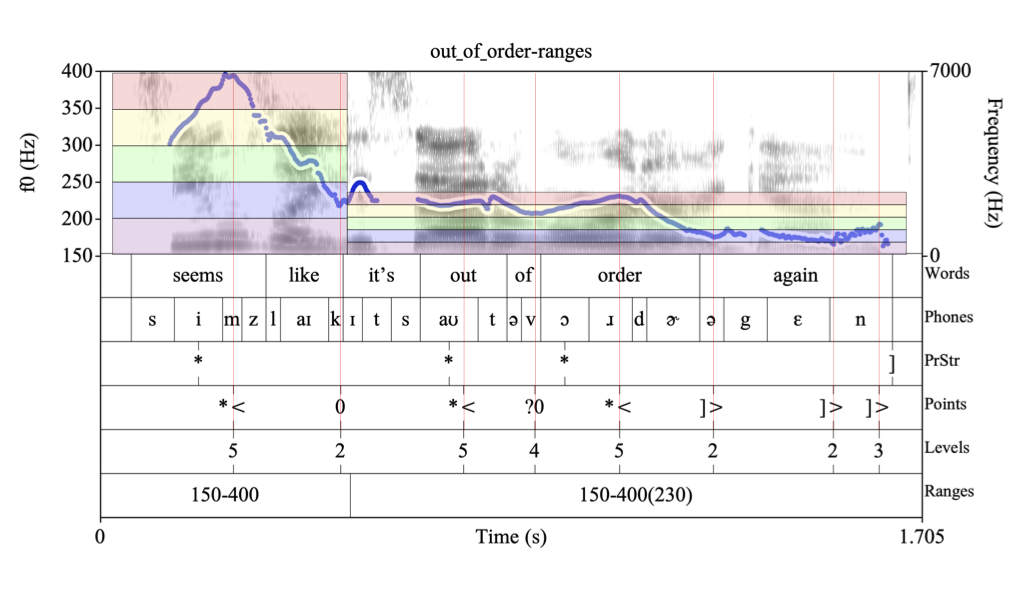
\includegraphics[width=.875\linewidth]{out_of_order-ranges-2RangeIntervals.png}
%
\caption{Parentheses labels are used to mark an advanced intuition that there is a second pitch range within what had been labelled as one pitch range by a labeller using PoLaR Basic labels.%
\label{fig:out_of_order-ranges 2range Ranges Adv}%
\index{Annotated example, Ranges tier (advanced)!out\_of\_order-ranges}
}
\end{figure}

These labels could be generated stepwise as follows. First, a labeller adding Basic Ranges labels could label the entire recording as one Ranges interval of “\textlabel{150-400}”; then, when an advanced labeller is adding more fine-grained labels, they notice the pitch range compression after “\langtext{seems like}” and so they divide the range in two, and in the second range they add a new, lower pitch ceiling label in parentheses: “\textlabel{150-400(230)}”. In other words, here the value in parentheses indicates \emph{the change} from the Basic label. Thus the advanced labeller has captured their intuition that the pitch range is compressed, in direct relation to the range labelled “\textlabel{150-400}” (i.e., that this is some kind of range compression operation that subordinates the latter range to the former one).

In this way, parentheses labels in the Ranges tier can be used both in cases where there is a second round of labelling (first Basic, then Advanced, as in this example), and where an advanced labeller initially captures global aspects of groups of ranges. (See section \ref{sec:sub-ranges-and-super-ranges-grouping-together-ranges-using-a-common-floor} on subranges and superranges for more on this.)

In the coming subsections, we discuss other commonly occurring contexts in which one may be motivated to annotate multiple Range intervals for a single utterance or prosodic phrase.

\subsection{Ranges and Pitch Floors}\label{sec:ranges-and-pitch-floors}

It has been observed that the pitch floor is typically more constant across long stretches, while the ceiling is much more variable: It is more likely that a labeller will find changes to the pitch range maximum, than they will to the pitch range minimum, especially within a particular utterance. (Though speakers do also make use of entirely different pitch ranges, with minima and maxima both differing, especially in cases of using falsetto voice or of intonationally distinguishing parenthetical speech, as discussed later in this section.) The observation that maxima vary more than minima, within speaker, is documented in \citealt{libermanpierrehumbert84}, which provides the following figure (\textit{ibid.}, p.159):

\begin{figure}[H]
\centering
%
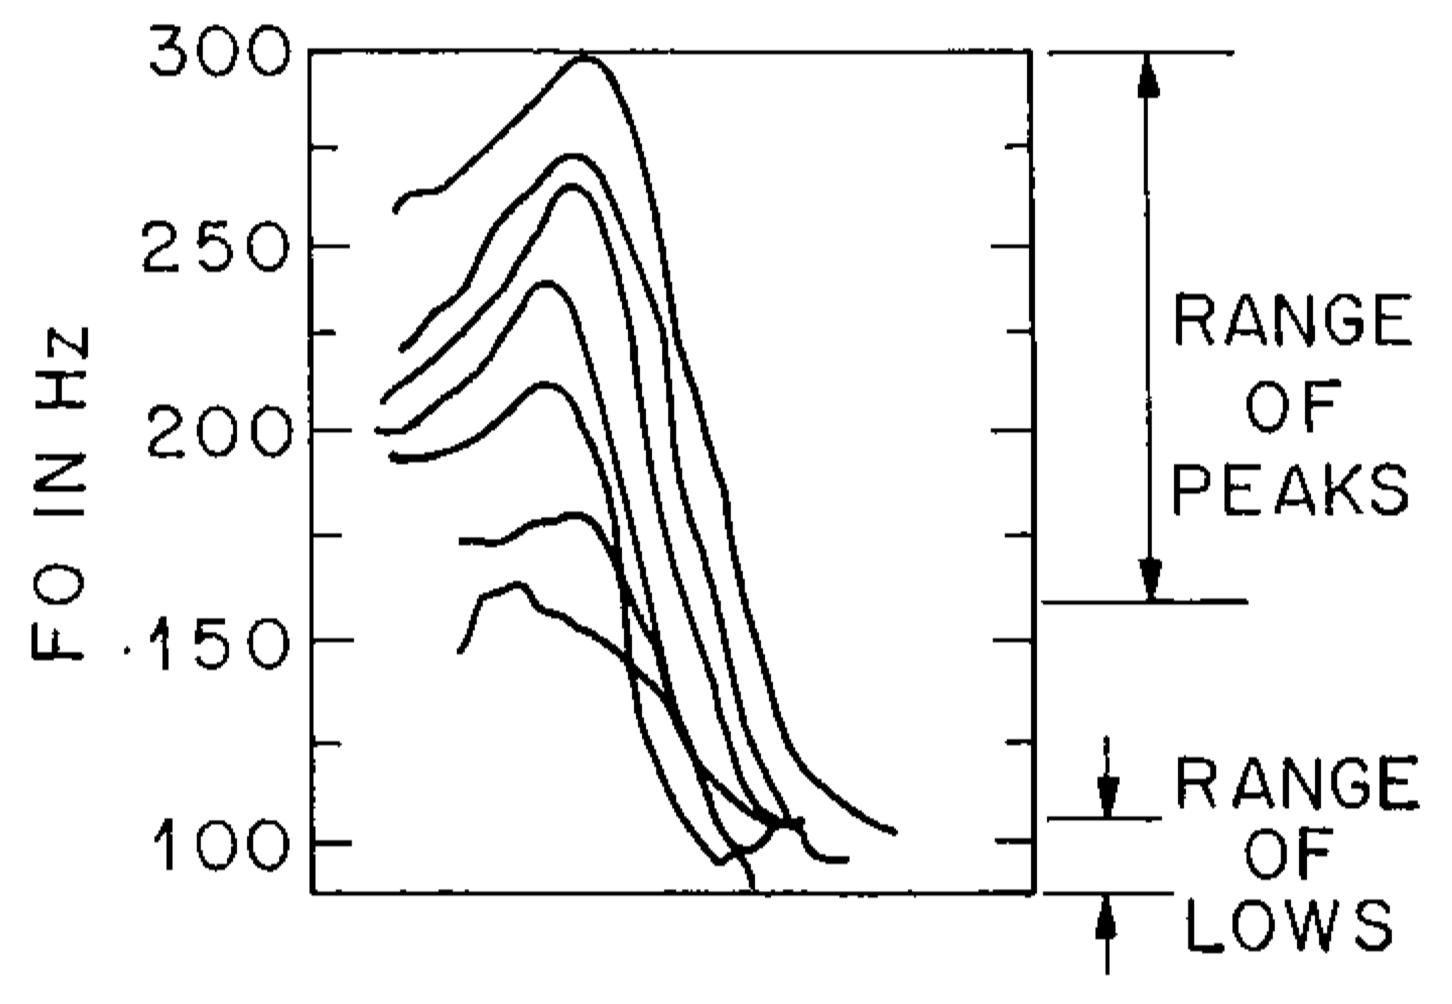
\includegraphics[height=2.75in]{LibermanPierrehumbert-Ranges.png}
%
\caption{Pitch maxima seem to vary more than pitch minima, for a given speaker.\textit{(From \citealt{libermanpierrehumbert84})}%
\label{fig:Liberman Pierrehumbert Ranges}%
}
\end{figure}

Thus, in cases where determining a pitch minimum is difficult (such cases described in the preceding sections), a labeller may be able to draw inferences about a pitch range minimum by elsewhere in recordings by the same speaker. For example, one could compare with other utterances by the same speaker where they use a similar pitch range and the pitch minimum is more easily measured. (In fact, a labeller might not need to look further than other parts of the same recording to find a more easily measured pitch minimum.) Additionally, if a large enough set of recordings for that speaker exists, a labeller might be able to get a sense of the speaker’s “normal” pitch range (its size, its floor, and/or its ceiling) and might be able to use this information to draw inferences about where the pitch minimum “should” be, even when difficult to measure directly.

\subsection{Some Trickier Cases with Local Pitch Ranges and Not-Attested Minimums}\label{sec:some-trickier-cases-with-local-pitch-ranges}

There are some fringe cases, which require deviation from the default approach, and where the labeller must attend to the more global context to identify the floor or ceiling. Not only will this deviation capture the labeller’s intuitions but the automatic Levels Tier algorithm will produce more useful results (more on this in the next section).

For example, the observed f0 minimum for a given interval does not always occur at the bottom of the local pitch range that the speaker gave themselves for a particular interval (i.e., the local minimum might not be a categorical “low”). This possibility raises an important question: how does an annotator know what to label as the mix\slash max for a local pitch range? As stated before in section \ref{sec:local-pitch-ranges-typical-cases}, the Basic Ranges default is to use the observed f0 points in the pitch contour as indicative of the minimum\slash maximum of the pitch range. However, you could imagine that a speaker may (in their mind) select a local pitch range but only ever produce observable pitch points in the high end of this range. As an example, an utterance may intonationally consist solely of high targets (e.g., a contour labelled in ToBI as /\textlabel{H* H* H-H\%}/). Such an example is provided in the figure below.

\begin{figure}[H]
\centering
%
\tikzset{
    dots/.style={
        line width=4pt,
        line cap=round,
        dash pattern=on 0pt off 6pt
    }
}
\begin{tikzpicture}[scale=1.25]
\draw (0,4.25) rectangle (5.25,1.5);
%\draw (0,1.5) rectangle (5.25,1);
%\node at (2.625, 1.25) {X-330};
\node[rotate=90] at (-0.75,2.875) {\relsize{-2}f0 (Hz)};
\begin{scope}[anchor=east, style={font=\relsize{-2}}]
%	\node at (0,0) {0};
%	\node at (0,1) {100};
	\node at (0,2) {200};
	\node at (0,3) {300};
	\node at (0,4) {400};
\end{scope}
\foreach \y in {2,...,4}
{
	\draw (0,\y) -- (-.1,\y);
}
\coordinate (pt1) at (0.2,3.1);
\coordinate (pt2) at (.7,3.3);
\coordinate (pt3) at (4.6,3.3);
\coordinate (pt4) at (5.1,3.6);
%\draw[fill] (pt1) circle (.05);
%\draw[fill] (pt2) circle (.05);
%\draw[fill] (pt3) circle (.05);
%\draw[fill] (pt4) circle (.05);
\draw[dots, CB1] (pt1) .. controls (pt2) .. (3,3.3) .. controls (pt3) .. (pt4);
\end{tikzpicture}
%\includegraphics[width=4in]{ranges-what-if3.png}
%
\caption{A hypothetical pitch track.%
\label{fig:ranges-what-if3 Ranges Adv}%
%\index{Annotated example, Ranges tier (advanced)!XXXXX}
}
\end{figure}

Assume that the labeller hears all these targets as high. As such, they have a good idea that the local pitch range max is something around 330Hz. At the same time, they see the local attested minimum value for the pitch is around 300Hz – labelling the Range as 300-330 would seem to miss the intuition that the minimum attested pitch sounds high.

In another case, a speaker may end up only producing pitch in the middle portion and high end of their selected local pitch range. For example, a speaker may start in the middle of this mental local pitch range, rise to high in that range, and fall to somewhere back to the middle of that range. An example of such a scenario is given Fig. \ref{fig:alejna2-nolabels}, for \texttt{alejna2} (we are assuming the speaker’s comfortable pitch range is 75Hz-450):

\begin{figure}[H]
\centering
%
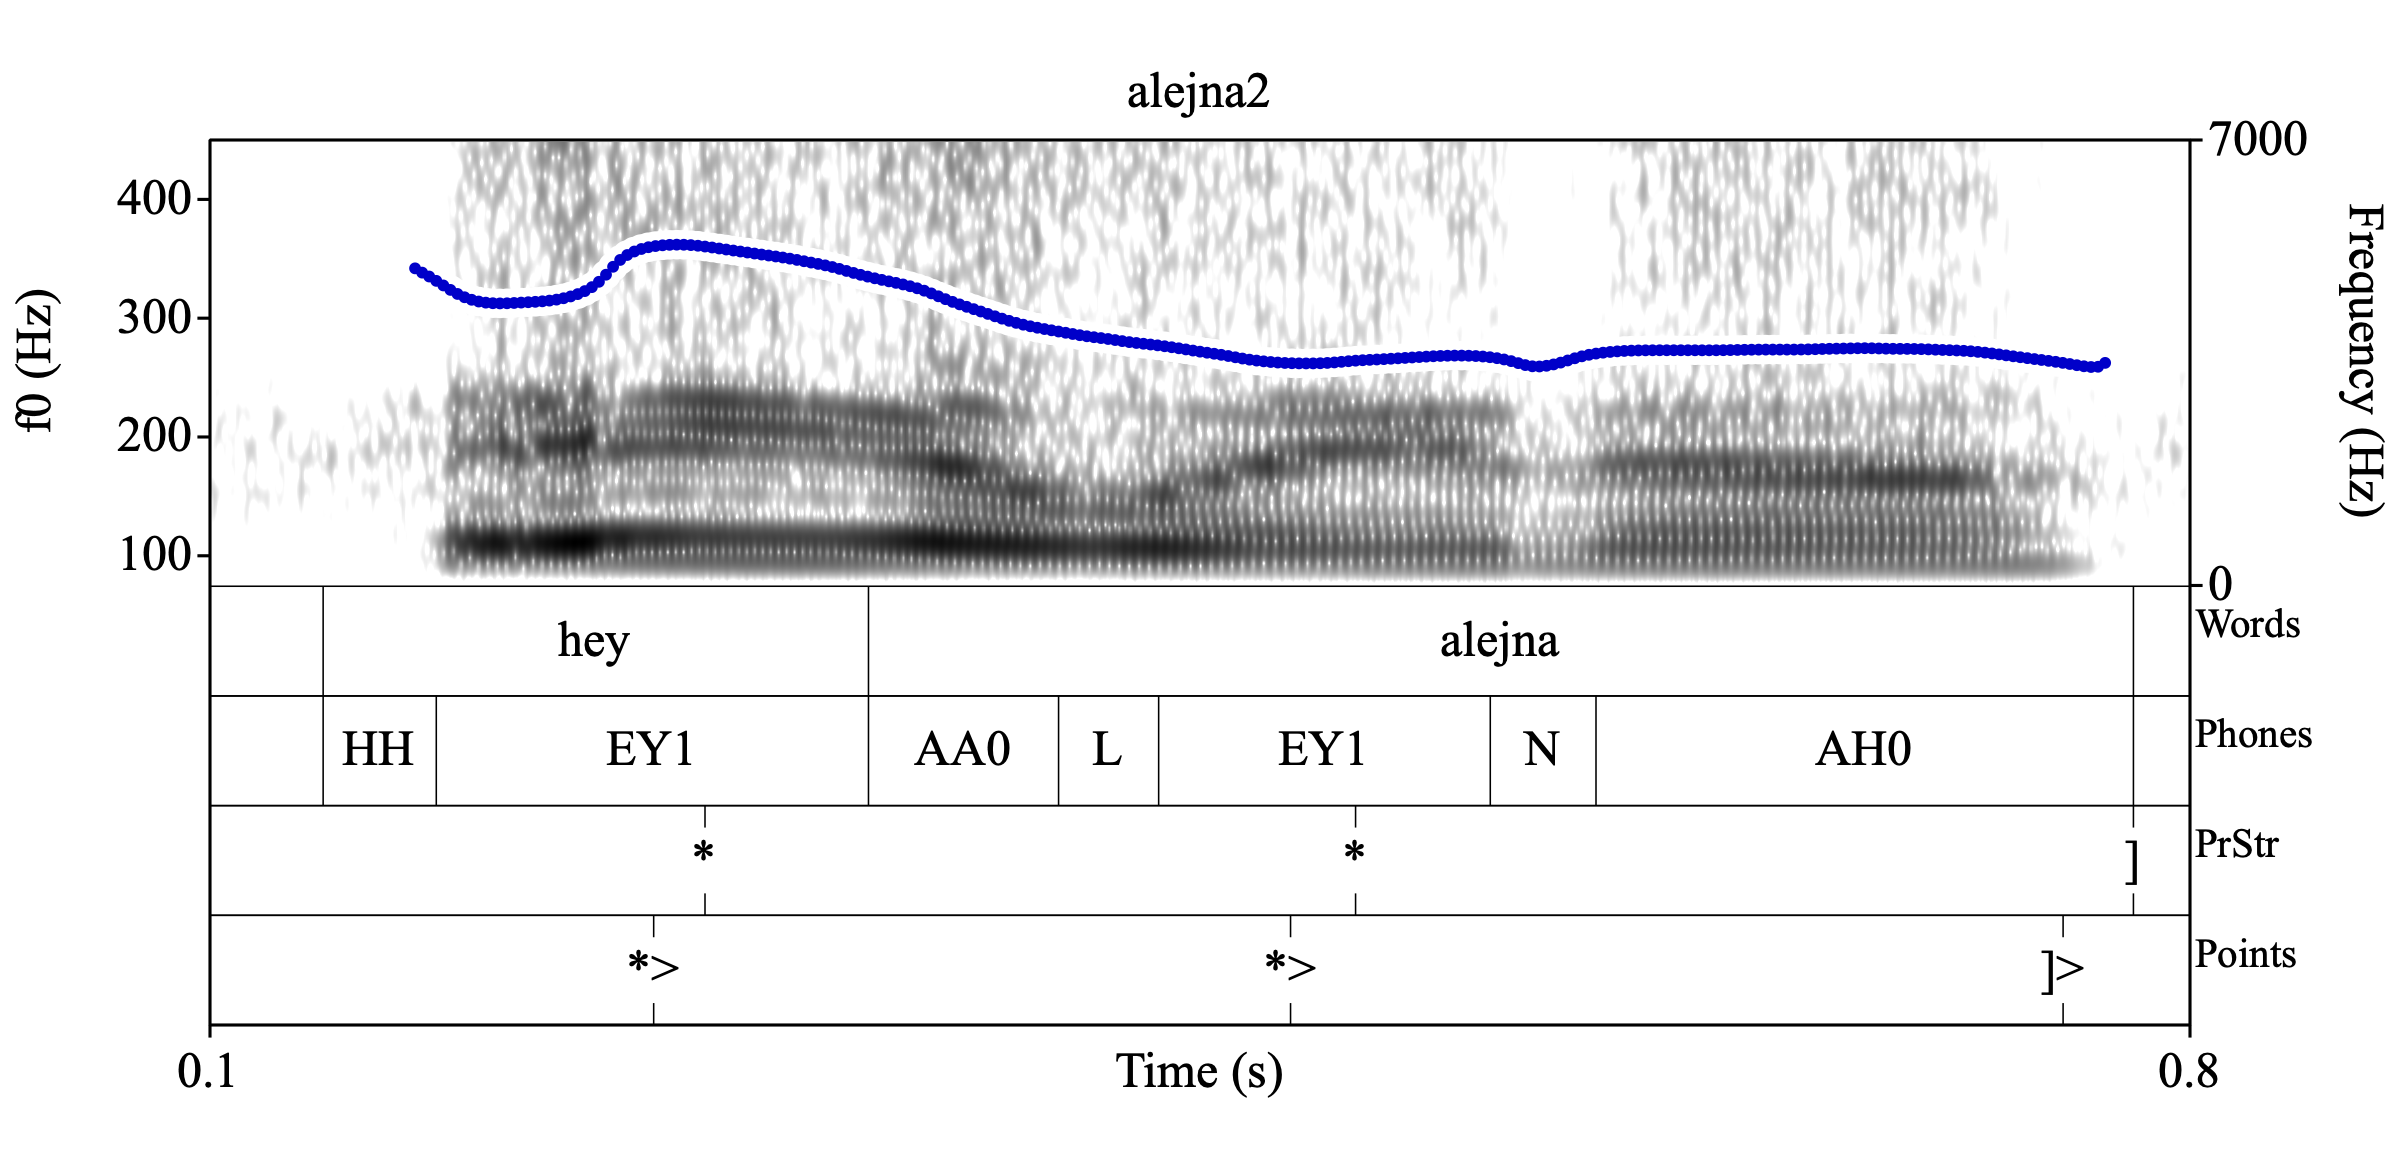
\includegraphics[width=.875\linewidth]{Ranges-alejna2-nolabels.png}
%
\caption{A recording with an attested pitch minimum of about 250Hz to 365Hz.%
\label{fig:alejna2-nolabels}%
\index{Annotated example, Ranges tier (advanced)!alejna2}
}
\end{figure}

On the basis of the f0 alone, the labeller would, by the default approach, label the interval as 250-365. However, it may be the case that the local pitch range (as represented in the mind of the speaker) is indeed something like 135Hz to 365Hz (meaning the speaker intended to never reach a “low” pitch – they fixed 135Hz as their pitch minimum, and only intended to reach a minimum of a “mid-level” pitch). This imagined scenario may be visualized as in the figure below, where each of the dots is an observable f0 point, and the box indicates the local pitch range for this utterance in the mind of the speaker. Note that none of the dots fall in the bottom portion of the range.

\begin{figure}[H]
\centering
%
\begin{tikzpicture}[scale=1.25]
\draw (0,4.5) -- (0,0.75) -- (1.8,.75);
%\node[anchor=south west] at (-0.9,-.2) {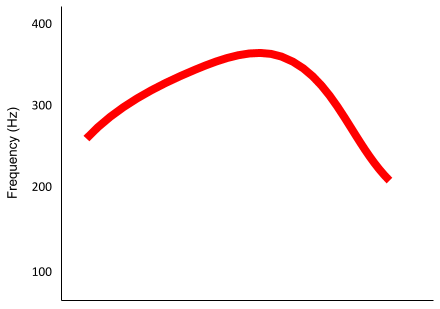
\includegraphics[scale=.4]{ranges-what-if1.png}};
\node[rotate=90] at (-0.75,2.2) {\relsize{-2}f0 (Hz)};
\begin{scope}[anchor=east, style={font=\relsize{-2}}]
	\node at (0,1) {100};
	\node at (0,2) {200};
	\node at (0,3) {300};
	\node at (0,4) {400};
\end{scope}
\foreach \y in {1,...,4}
{
	\draw (0,\y) -- (-.1,\y);
}

\draw[fill=CB1!40] (.3,1.35) rectangle (1.5,3.65);
\coordinate (pt1) at (0.925,3.6);
\coordinate (pt2) at (.825,3.57);
%
\coordinate (pt3) at (.885,3.48);
\coordinate (pt4) at (.933,3.23);
\coordinate (pt5) at (1.05,3);
\coordinate (pt6) at (0.85,2.9);
\coordinate (pt7) at (0.925,2.7);
%
\coordinate (pt8) at (.65,2.62);
\coordinate (pt9) at (0.75,2.58);
\coordinate (pt10) at (.85,2.6);
\coordinate (pt11) at (.95,2.6);
\coordinate (pt12) at (1.05,2.55);
\coordinate (pt13) at (1.15,2.65);
\foreach \x in {1,...,13}
{
\draw[fill] (pt\x) circle (.04);
}
%
\end{tikzpicture}
%\includegraphics[width=2in]{ranges-what-if2.png}
%
\caption{The filled box indicates the speaker’s intended local pitch range, and the black dots indicate f0 observations.%
\label{fig:ranges intuition alejna2}%
%\index{Annotated example, Ranges tier (advanced)!XXXXX}
}
\end{figure}

What this figure reflects is an intuition that the speaker did not reach the bottom of their local pitch range (i.e., that the speaker did not produce a low pitch in this utterance).

This would mean that in examples like Fig. \ref{fig:ranges-what-if3 Ranges Adv} and Fig. \ref{fig:alejna2-nolabels}) there are \uline{no local acoustic cues} for determining even an approximation of the local pitch range minimum. This is because only a portion of the speaker’s local pitch range is actually attested by the f0 contour (e.g., the speaker is using only high, or only low, pitch targets). To be clear, this means there are cases where the labeller ought to \uline{deviate from the default practice} of using observed f0 for deciding local pitch range max\slash min.

To allow for this, we provide a convention to capture that there are “unused” portions of the local pitch range, while also preserving what the attested values for the pitch range min\slash max are. In these cases, the labeller should label the pitch min\slash max with the attested value plus an educated guess for the “actual” floor\slash ceiling value plus “\textlabel{:na}” (for “not attested”).

Solely on the basis of observed f0, a labeller would label the Range interval as “250-365”. Using this convention and matching the intuition described in Fig. \ref{fig:ranges intuition alejna2}, we add “\textlabel{(135:na)}”, as below, to indicate that the pitch space extends down to 135Hz, even though no measured f0 is attested between 135Hz and 250Hz. 

\begin{figure}[H]
\centering
%
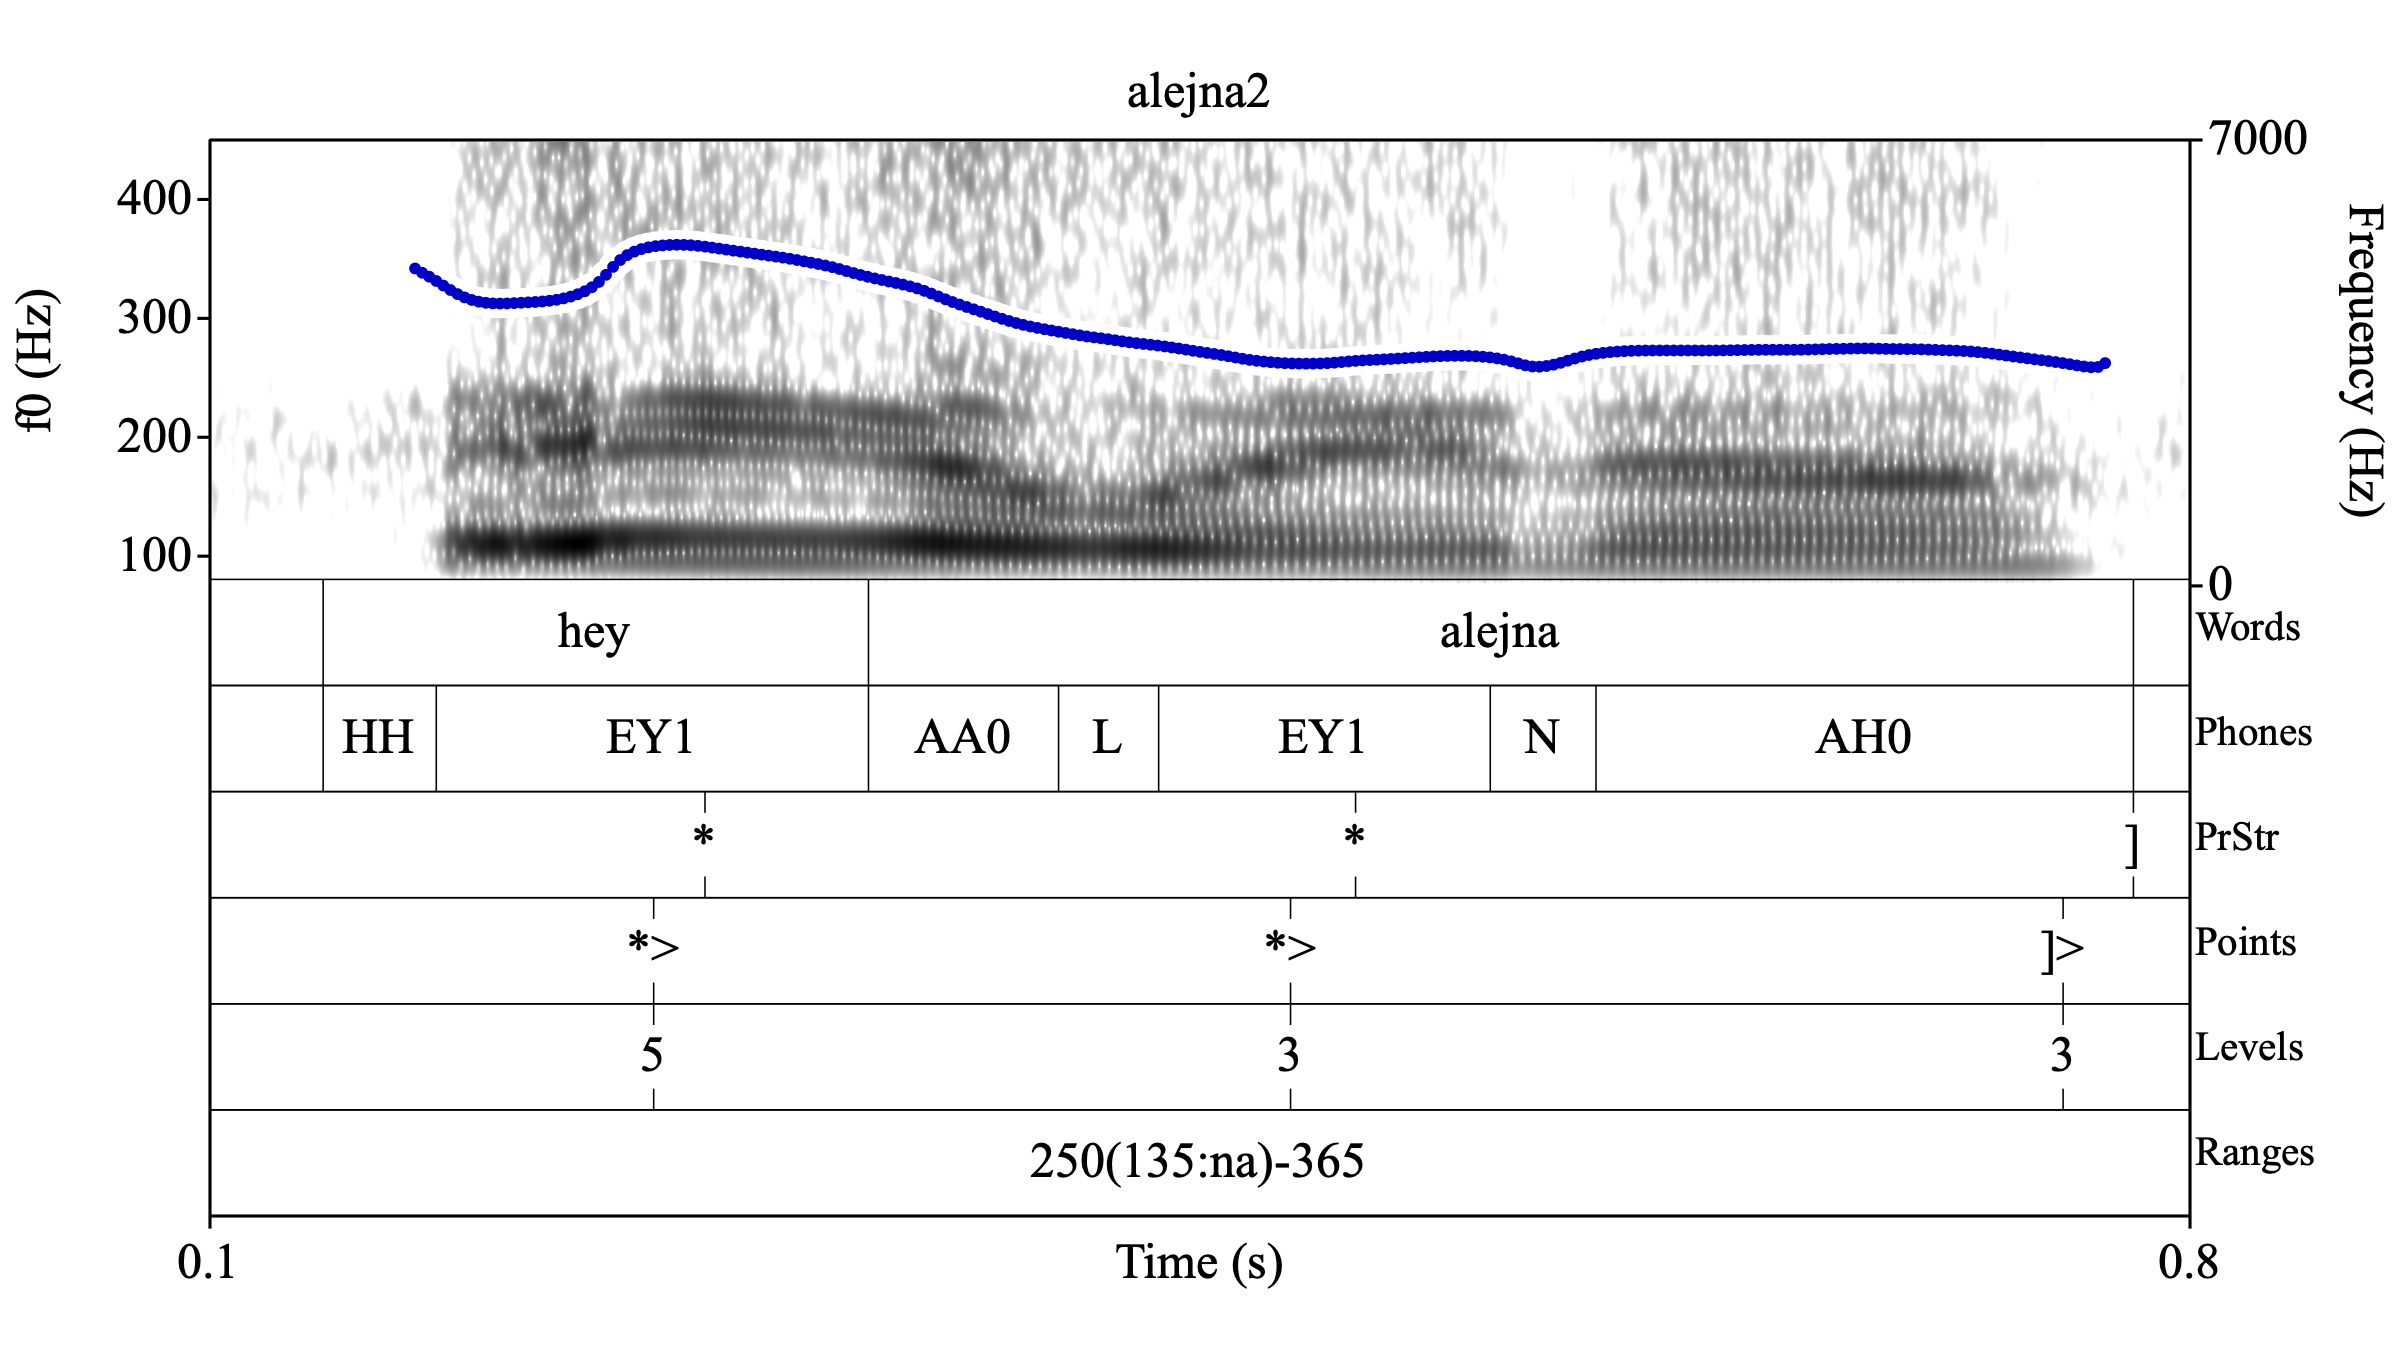
\includegraphics[width=.875\linewidth]{Ranges-alejna2.png}
%
\caption{Labels capturing the intuition that the pitch range minimum (intuited as 135Hz) is not attested in the f0 track.%
\label{fig:alejna2 na}%
\index{Annotated example, Ranges tier (advanced)!alejna2}
}
\end{figure}

We must recognize that the value for the unattested minimum is meant to be an educated guess. We provide some guidance on how to best arrive at such a guess.

First, a labeller may know what this particular speaker sounds like when they produce a low – perhaps pulling from information about the speaker’s prosody in other cases (e.g., phonation, lengthening, or local pitch range size). Using this more global\footnote{In the data analysis, if there is enough data from the same speaker, it may be possible to reconstruct what the pitch min is in cases like this (e.g., on the basis of normal pitch range sizes).} information, a labeller may have the sense after listening to this particular recording that the pitch at 250Hz in this context is \emph{\uline{not}} the speaker’s low (even if 250Hz is this speaker’s low elsewhere, in other recordings). 

Second, if a labeller hears the end of the utterance being in the middle of the pitch range, the labeller can do some simple arithmetic along the following reasoning: “250Hz is in the middle of the range, if the maximum is 365Hz, the minimum should be about equidistant from 250Hz – 135Hz.” Of course, a range of values would yield this same result of 250Hz being somewhere in the middle of the pitch range, so the labeller might just as well label this Range as “\textlabel{250(160:na)-365}” or something else, if it aligns with other more global information better than 135Hz as the pitch range minimum. (We return in the next section to using Levels values as a sanity check on Ranges labels, in a similar way.)

Another similar example with this “\textlabel{:na}” label is provided with \texttt{minimum2}.

\begin{figure}[H]
\centering
%
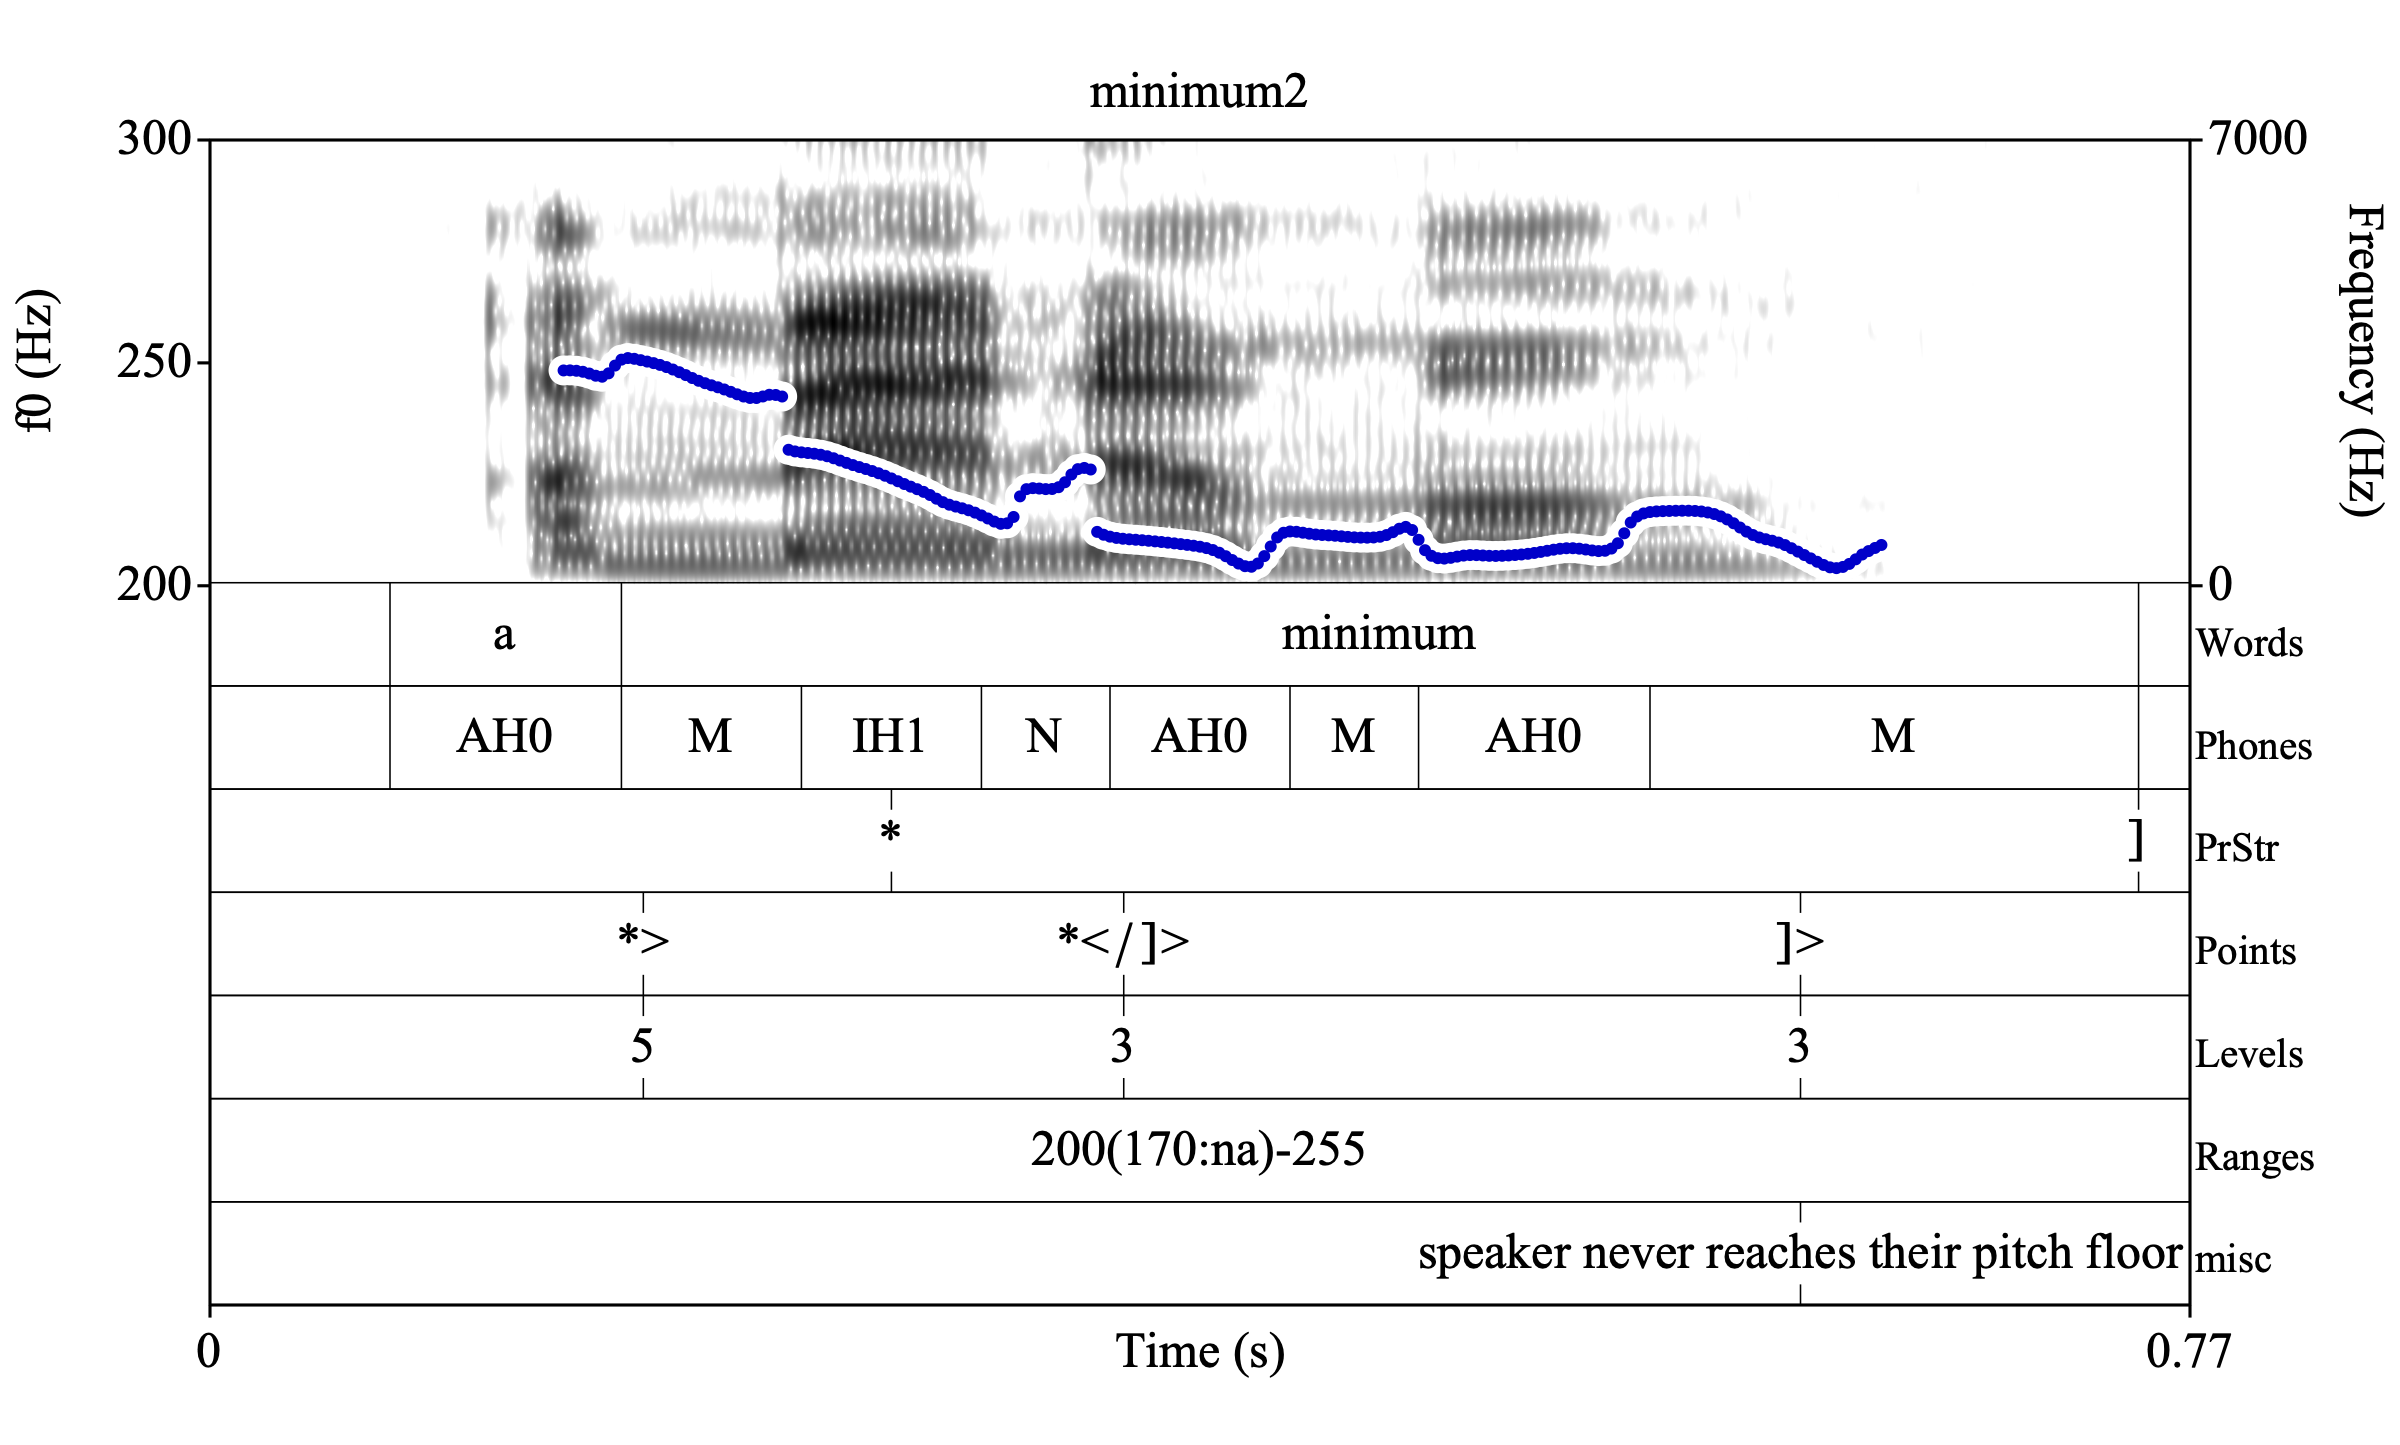
\includegraphics[width=.875\linewidth]{Ranges-minimum2-ranges-adv.png}
%
\caption{Labels capturing the intuition that the pitch range minimum (intuited as 170Hz) is not attested in the f0 track.%
\label{fig:minimum2 Ranges Adv}%
\index{Annotated example, Ranges tier (advanced)!minimum2}
}
\end{figure}

Here the labellers hear the pitch as falling to a steady mid-level, and not to a steady low, and so the lower half of the pitch range must not be attested by the f0 contour.

Another case where the labeller may want to use their ear is when the pitch track becomes untrackable or unreliable. For example, in an example like raining-ranges, labellers report being able to hear the pitch continuing to fall, even after “\langtext{raining}”, where the pitch track gets lost and/or becomes unreliable because of issues with voice quality. (i.e., Here the labeller knows that the end of “\langtext{there}” is not higher than “\langtext{raining}”, so the tracked pitch must be erroneous.)

\begin{figure}[H]
\centering
%
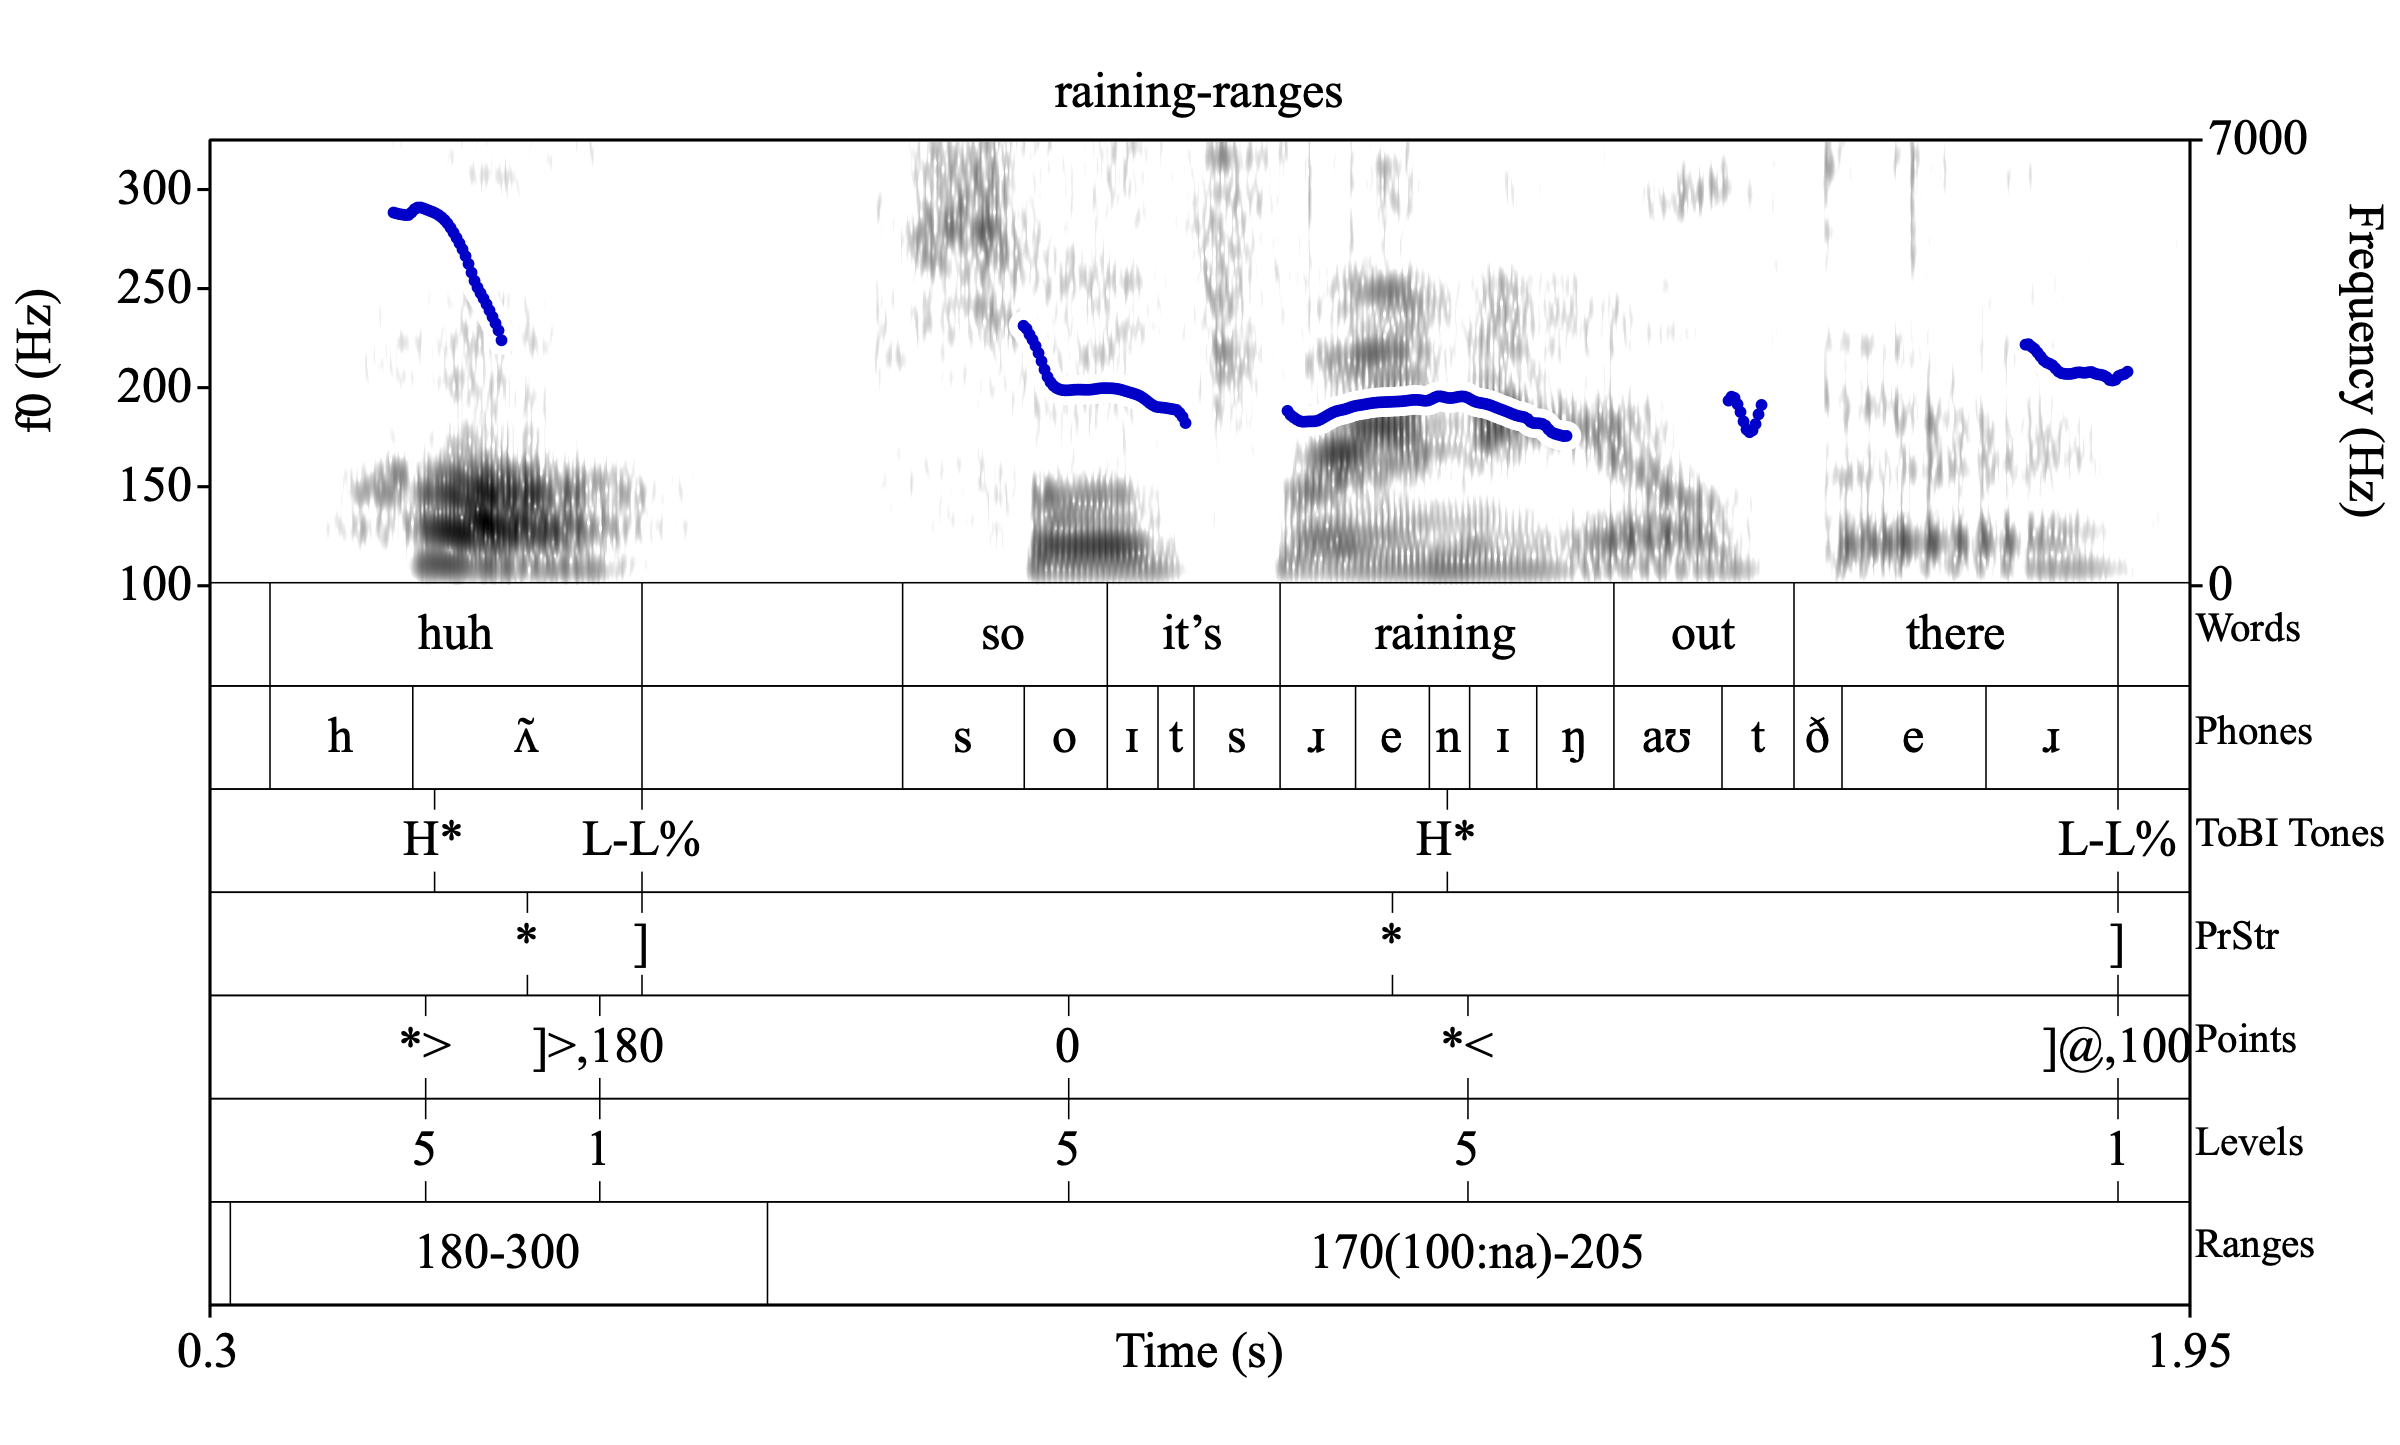
\includegraphics[width=.875\linewidth]{Ranges-raining-ranges-adv.png}
%
\caption{The labeller provides an educated guess of the pitch minimum during “\langtext{out there}”.%
\label{fig:raining-ranges Ranges Adv}%
\index{Annotated example, Ranges tier (advanced)!raining-ranges}
}
\end{figure}

Here the f0 measured at the end of “\langtext{there}” is measured as around 200Hz; as this might be an instance of pitch doubling, an educated guess for the final f0 may be 100Hz (as indicated by the comma-override), but the lowest reliable f0 (towards the end of “\langtext{raining}”) is around 170Hz. This leads to the Ranges label of “\textlabel{170(100:na)-205}”.

Finally, there are cases where there is what seems to be an entire Range interval where there is no (reliable) f0 tracking (e.g., because of low recording quality, or non-modal phonation). To be clear, this is intended to identify cases where the labeller has no visual cues to the pitch values, perhaps because the software-generated f0 track is missing or is tracked at the wrong pitch height (as determined by the labeller’s ear) for a long stretch of time, as in the figure below:

\begin{figure}[H]
\centering
%
\tikzset{
    dots/.style={
        line width=4pt,
        line cap=round,
        dash pattern=on 0pt off 6pt
    }
}
\begin{tikzpicture}[scale=1.25]
%\node[anchor=north west, xscale=.225, yscale=.225] at (-0.525,4.15) {\includegraphics{ranges-what-if4.png}};
\node[rotate=90] at (-0.75,3) {\relsize{-2}f0 (Hz)};
\begin{scope}[anchor=east, style={font=\relsize{-2}}]
%	\node at (0,0) {0};
%	\node at (0,1) {100};
	\node at (0,2) {200};
	\node at (0,3) {300};
	\node at (0,4) {400};
\end{scope}
\foreach \y in {2,...,4}
{
	\draw (0,\y) -- (-.1,\y);
}
\begin{scope}
\draw (0,4.25) rectangle (7.75,1.75);
\draw (0,1.75) rectangle (3.5,1.25);
\node at (1.75, 1.5) {\relsize{-2}220-350};
\draw (3.5,1.75) rectangle (7.75,1.25);
\node at (5.625, 1.5) {\relsize{-2}(100:na)-(220:na)};
\coordinate (pt1) at (0.2,2.5);
\coordinate (pt2) at (.7,3.4);
\coordinate (pt3) at (1.4,2.35);
\coordinate (pt4) at (2,2.75);
\coordinate (pt5) at (2.35,2.25);
\coordinate (pt6) at (2.75,2.22);
\coordinate (pt7) at (4.75,2.1);
\coordinate (pt8) at (4.85,2.2);
\coordinate (pt9) at (5.05,1.95);
\coordinate (pt10) at (6.7,3.75);
\coordinate (pt11) at (6.85,3.75);
\coordinate (pt12) at (6.9,3.65);
\coordinate (pt13) at (7.3,3.85);
\coordinate (pt14) at (7.4,3.75);
%\foreach \x in {1,...,14}
%{
%	\draw[fill] (pt\x) circle (.05);
%}
\draw[CB1, dots] (pt1) sin (pt2) cos ([xshift=-7,yshift=10]pt3) sin (pt3) cos ([xshift=7,yshift=5]pt3) sin  (pt4) cos ([xshift=-5,yshift=7]pt5) sin (pt5) -- (pt6);
\draw[CB1, dots] (pt7) .. controls (pt8) .. (pt9);
\draw[CB1, dots] (pt10) .. controls (pt11) and (pt12) .. ([xshift=-3]pt13) .. controls (pt13) .. (pt14);
\end{scope}
\end{tikzpicture}
%\includegraphics[width=4in]{ranges-what-if4.png}
%
\caption{A hypothetical pitch track.%
\label{fig:ranges-what-if4 Ranges Adv}%
%\index{Annotated example, Ranges tier (advanced)!XXXXX}
}
\end{figure}

Here, the labeller thinks they are hearing the f0 as all lower than 220Hz (the previous range minimum), and is providing an educated guess (perhaps based on other recordings by this speaker) that the minimum is at 100Hz. However, the labeller does not want to commit to saying there are any attested f0 values, and so they have given a label where there are no pitch range values outside of the parentheses. Thus in all cases, labellers ought to give Ranges labels – even if made up entirely of guesses for which the f0 min\slash max are not attested directly in the f0 contour.

As a contrast with Fig. [fig:ranges what if 4], consider Fig. \ref{fig:ranges-what-if5 Ranges Adv}, where the f0 track becomes unreliable but it \emph{does} recover (and the labeller hears it as the same local pitch range throughout), there is no need to add any “\textlabel{:na}” labels (assuming the labeller does not hear any dip in pitch during the interval where no f0 is measured by the software).

\begin{figure}[H]
\centering
%
\tikzset{
    dots/.style={
        line width=4pt,
        line cap=round,
        dash pattern=on 0pt off 6pt
    }
}
\begin{tikzpicture}[scale=1.25]
%\node[anchor=north west, xscale=.225, yscale=.225] at (-0.525,4.15) {\includegraphics{ranges-what-if5.png}};
\node[rotate=90] at (-0.75,3) {\relsize{-2}f0 (Hz)};
\begin{scope}[anchor=east, style={font=\relsize{-2}}]
%	\node at (0,0) {0};
%	\node at (0,1) {100};
	\node at (0,2) {200};
	\node at (0,3) {300};
	\node at (0,4) {400};
\end{scope}
\foreach \y in {2,...,4}
{
	\draw (0,\y) -- (-.1,\y);
}
\begin{scope}
\draw (0,4.25) rectangle (7.75,1.75);
\draw (0,1.75) rectangle (7.75,1.25);
\node at (3.875, 1.5) {\relsize{-2}220-350};
\coordinate (pt1) at (0.2,2.5);
\coordinate (pt2) at (.7,3.4);
\coordinate (pt3) at (1.4,2.35);
\coordinate (pt4) at (2,2.75);
\coordinate (pt5) at (2.35,2.25);
\coordinate (pt6) at (2.75,2.22);
\coordinate (pt7) at (5.3,2.25);
\coordinate (pt8) at (6.4,2.25);
\coordinate (pt9) at (7.45,2.2);
%\foreach \x in {1,...,9}
%{
%	\draw[fill] (pt\x) circle (.05);
%}
\draw[CB1, dots] (pt1) sin (pt2) cos ([xshift=-7,yshift=10]pt3) sin (pt3) cos ([xshift=7,yshift=5]pt3) sin  (pt4) cos ([xshift=-5,yshift=7]pt5) sin (pt5) -- (pt6);
\draw[CB1, dots] (pt7) .. controls (pt8) .. (pt9);
\end{scope}
\end{tikzpicture}
%\includegraphics[width=4in]{ranges-what-if5.png}
%
\caption{A hypothetical pitch track.%
\label{fig:ranges-what-if5 Ranges Adv}%
%\index{Annotated example, Ranges tier (advanced)!XXXXX}
}
\end{figure}

\subsection{Sub-ranges and super-ranges: Grouping together ranges using a common floor}\label{sec:sub-ranges-and-super-ranges-grouping-together-ranges-using-a-common-floor}

In labelling the ranges of longer stretches of speech containing multiple ranges, the labeller may have the intuition that two or more nearby ranges (often consecutive, but not necessarily so) are related tonally, and form part of a larger group. For labellers who have such intuitions and wish to capture them, they are encouraged to indicate this relationship by labelling related ranges with the same Ranges minimum value.

The figure below shows an example of a speaker producing a sequence of phrases produced with distinct pitch ceilings. The first range covers quite a short duration, and contains a single word, as well as just one phrase and prominence as marked in the PrStr tier. If a labeller were to only see this part of the utterance, it might seem like the floor should be around the lowest point of this particular group, i.e., the beginning of the utterance, or around 260Hz. This would suggest that the pitch movement, at the beginning of the word “\langtext{this}” goes from the local low to the local high. However, when the rest of the utterance is taken into consideration, the labeller’s  intuition might be that the three ranges form part of the same larger tonal group and this can be captured, as it is here, by giving all intervals the same pitch floor of 130Hz. Further, this common-floor approach captures the sense that the word “\langtext{this}” does not sound as though it starts at a real local low in the speaker’s range – but rather somewhere in the middle of their range. By choosing the floor from the observed pitch track in the subsequent ranges, the labeller captures both the intuitions about the floor of the first range, but also that the three ranges form part of the same tune or melody, i.e., some larger tonal group.

\begin{figure}[H]
\centering
%
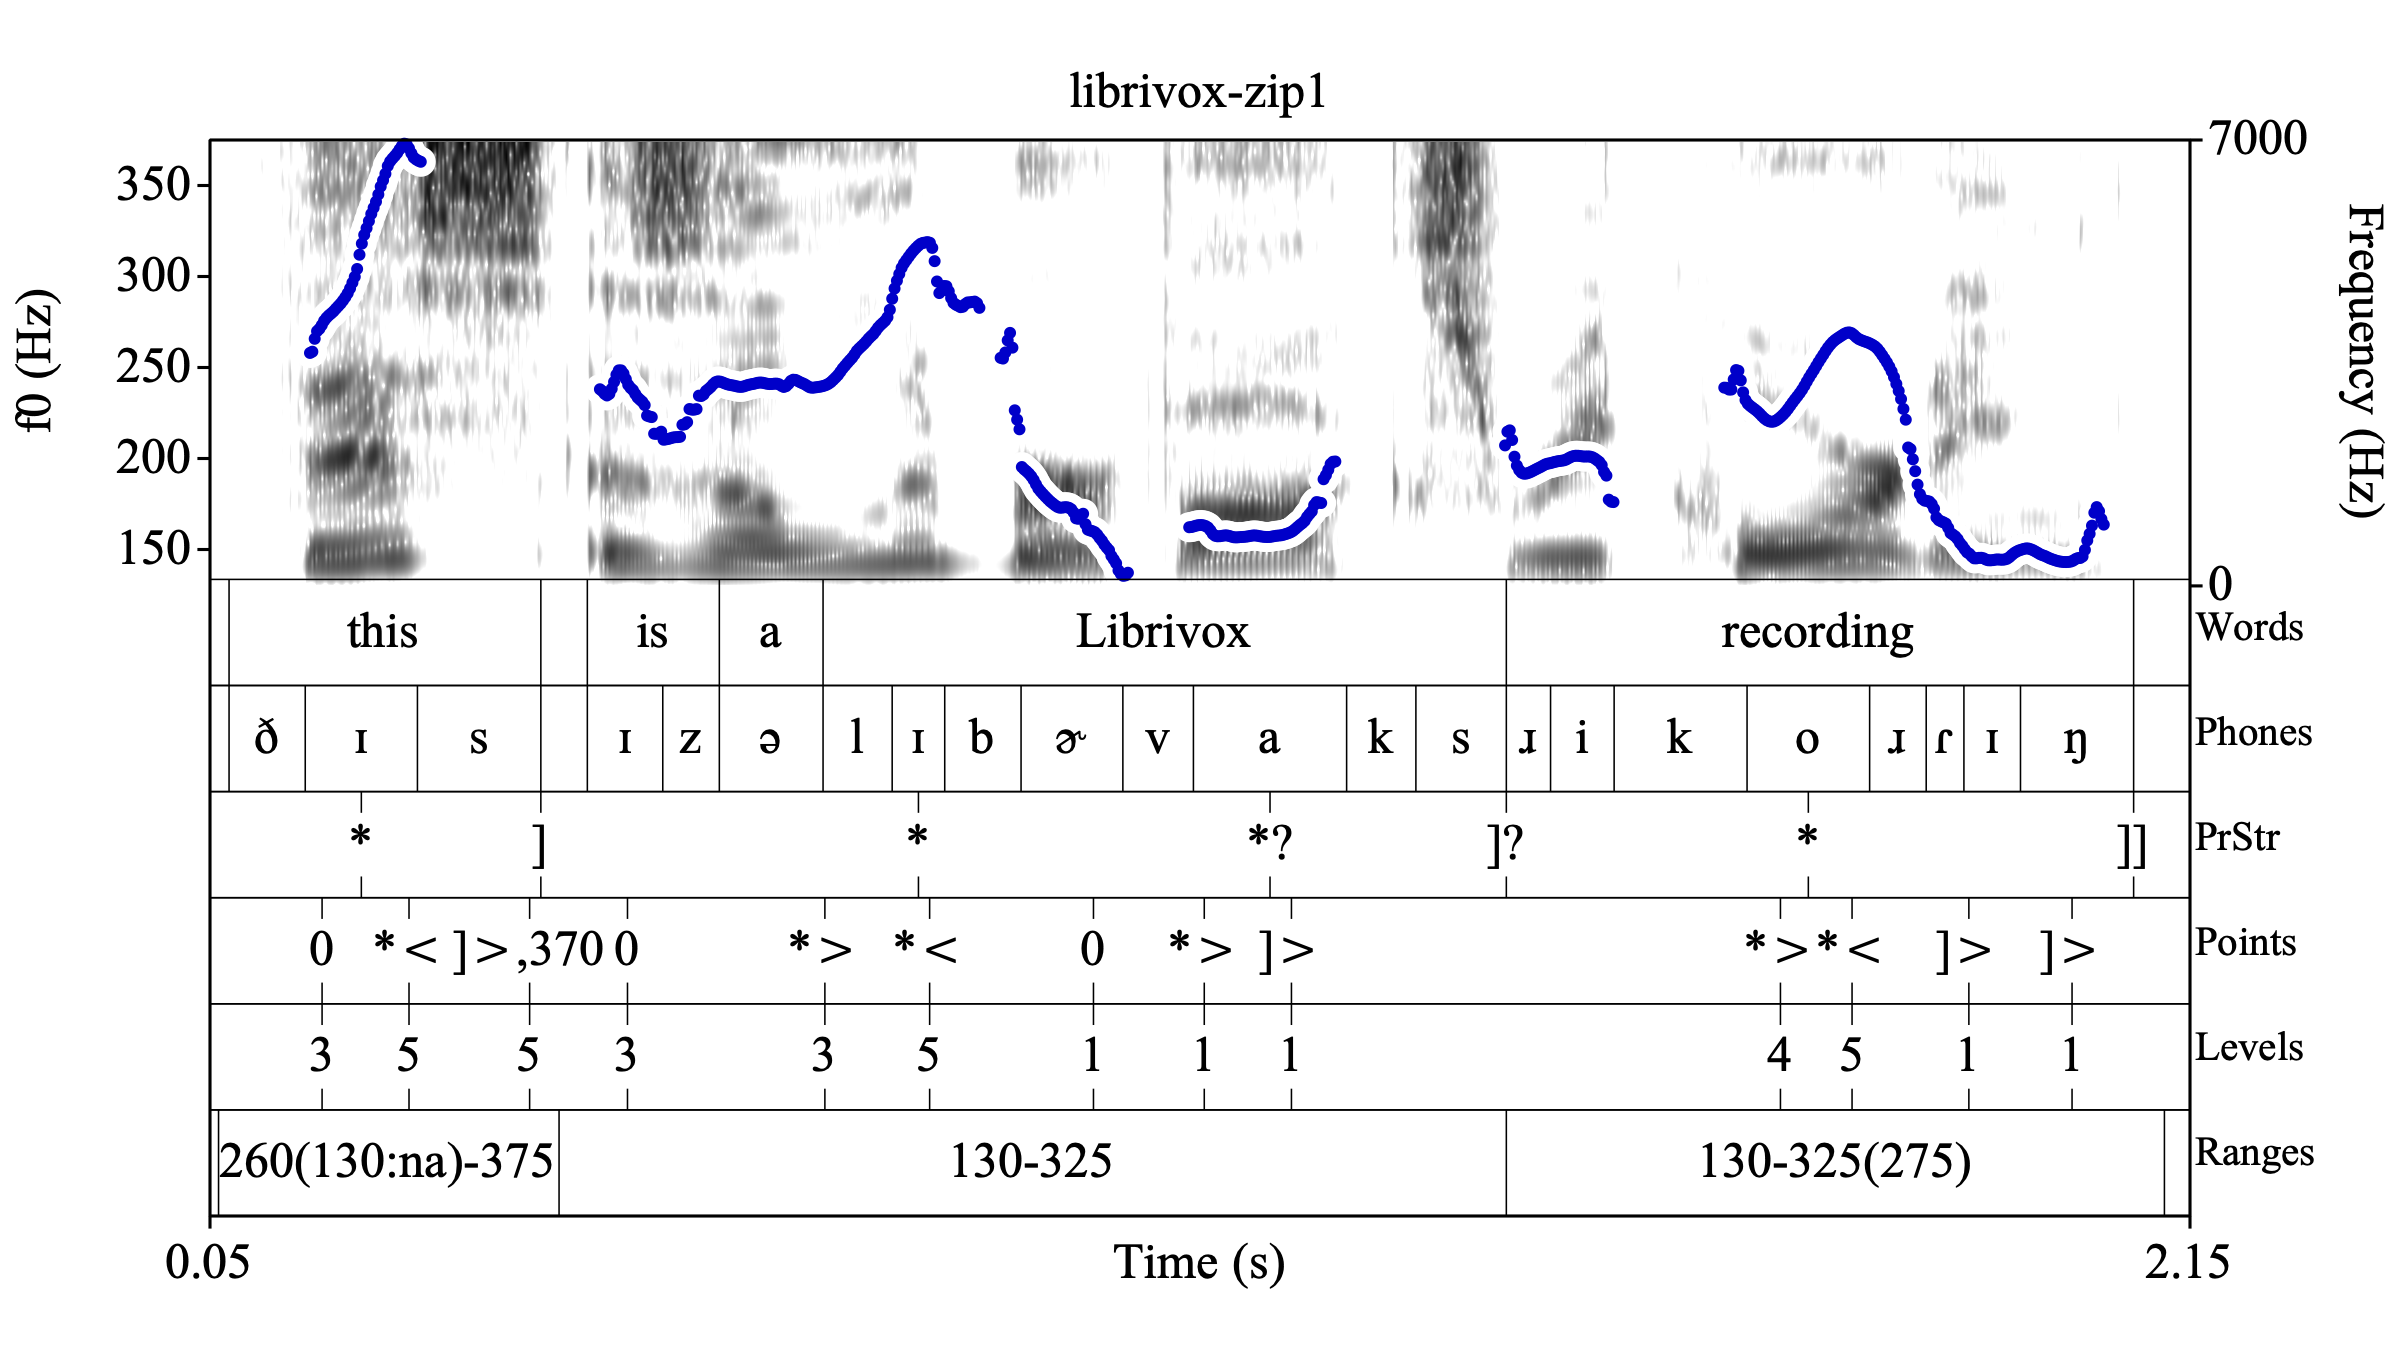
\includegraphics[width=.875\linewidth]{Ranges-librivox-zip1-adv.png}
%
\caption{\texttt{librivox-zip1}, with Advanced PoLaR labels.%
\label{fig:librivox-zip1 Ranges Adv}%
\index{Annotated example, Ranges tier (advanced)!librivox-zip1}
}
\end{figure}

This example further illustrates varying approaches to labelling the Ranges tier, and their effects. For instance, one labeller might consider that there is only one local pitch range for the whole short utterance, such as 130-375. Another labeller might want to capture three ranges, one for each of the three prosodic phrases, where both the ceiling and floor are determined locally, on the basis of what the listener can observe\slash intuit about pitch minima and maxima in the time span. A third approach (and the one used to label Figure \ref{fig:librivox-zip1 Ranges Adv}) could be considered a hybrid of these approaches: the pitch maxima are locally determined based on observations\slash intuition, while the use of a ‘shared’ pitch minimum captures the intuition that the phrases form part of some hierarchically superior tonal group. It is left to individual labellers to determine whether they want to capture the granularity of ranges in an utterance and the relationships between them. As we will see below, these choices can impact the automatic Levels Tier labels.

\subsection{Summary of the Advanced Labels for the Ranges Tier}\label{sec:summary-advanced-ranges-labels}
\begin{longtable}{cp{.46\linewidth}p{.32\linewidth}} \toprule \textbf{Label} & \textbf{Phonological Object} & \textbf{Example}\tabularnewline
\midrule \endhead
\rowcolor{green}
{[\textit{min}]-[\textit{max}]} &
	{[\textit{min}] is the local pitch minimum, in Hertz, rounded down to a nearby number ending in a 5 or a 0}; {[\textit{max}] is the local pitch maximum, in Hertz, rounded up to a nearby number ending in a 5 or a 0} &
	If the local pitch min is 244.2Hz and the local pitch maximum is 381.5Hz, the label should be ‘\textlabel{240-385}’
	\tabularnewline
{[\textit{min}]([\textit{min2}]:na)} &
	[\textit{min}] is the Basic ranges value for the minimum, and [\textit{min2}] (written in parentheses) is the Advanced ranges label, capturing labeller intuitions for a value that is not attested locally within that interval &
	If the local attestable pitch min is 112, but the labeller intuits that the speaker has deliberately not reached a low ‘\textlabel{110(90:na)-385}’
	\tabularnewline
{[\textit{max}]([\textit{max2}]:na)} &
	[\textit{max}] is the Basic ranges value for the minimum, and [\textit{max2}] (written in parentheses) is the Advanced ranges label, capturing labeller intuitions for a value that is not attested locally within that interval &
	If the local attestable pitch min is 192, but the labeller intuits that the speaker has deliberately not reached a high ‘\textlabel{90-192(300:na)}’
	\tabularnewline
{\textlabel{X-}[\textit{max}]} &
	{“X” represents a pitch minimum that the labeller cannot determine}; {[\textit{max}] is the local pitch maximum, in Hertz, rounded up to a nearby number ending in a 5 or a 0}	 &
	If the local pitch max is 264.8Hz and the local pitch maximum is not easy to determine, the label should be ‘\textlabel{X-270}’
	\tabularnewline
{[\textit{min}]\textlabel{-X}} &
	{[\textit{min}] is the local pitch minimum, in Hertz, rounded up to a nearby number ending in a 5 or a 0}; {“X” represents a pitch maximum that the labeller cannot determine}	 &
	If the local pitch min is 138.2Hz and the local pitch maximum is not easy to determine, the label should be ‘\textlabel{135-X}’
	\tabularnewline
\textlabel{NA} &
	“NA” indicates a stretch of unreliable pitch tracking, in places where surrounding information cannot be used to infer the pitch range minimum\slash maximum (\textit{To be used in last resort scenarios}) &
	If the pitch is a long stretch of unreliable pitch tracking, the label for that unreliable stretch is ‘\textlabel{NA}’
	\tabularnewline
\bottomrule 
\caption[An expanded set of labels for the Ranges tier.]{An expanded set of labels for the Ranges tier. The fundamental label is highlighted, with the remaining labels being for recordings with less clear pitch tracking.}
\end{longtable}


%[[XXX COMMENTS TO BE REMOVED:]] ToBI-related text removed from Ranges (Advanced) section, concatenated, smoothed and diplomaticized (SSH 10-2-20; original texts shown at the end of this concatenated-smoothed version

\subsection{Some English Pitch Range Phenomena}\label{sec:some-english-pitch-range-phenomena}

In this section, we discuss some phenomena whereby pitch ranges are “shifted”, “expanded”, or “compressed”. In particular, we focus on examples from American English, and propose some Advanced labels to capture these phenomena.

\subsubsection{Range Compression: a commonly-occurring local range change}\label{sec:range-compression-a-commonly-occurring-local-range-change}

A commonly occurring context which corresponds to a change in local pitch range is when a tonal event is perceived as locally high in pitch, but is lower than a preceding high tonal event, which we will describe as “range compression”. A particular type of range compression includes what is commonly known as intonational “downstep”, which is where a perceptually high tonal target occurs at a (significantly) lower pitch than a preceding high tonal target. An example of this was given earlier, and is repeated in Figure \ref{fig:out_of_order-ranges Ranges Adv}.

\begin{figure}[H]
\centering
%
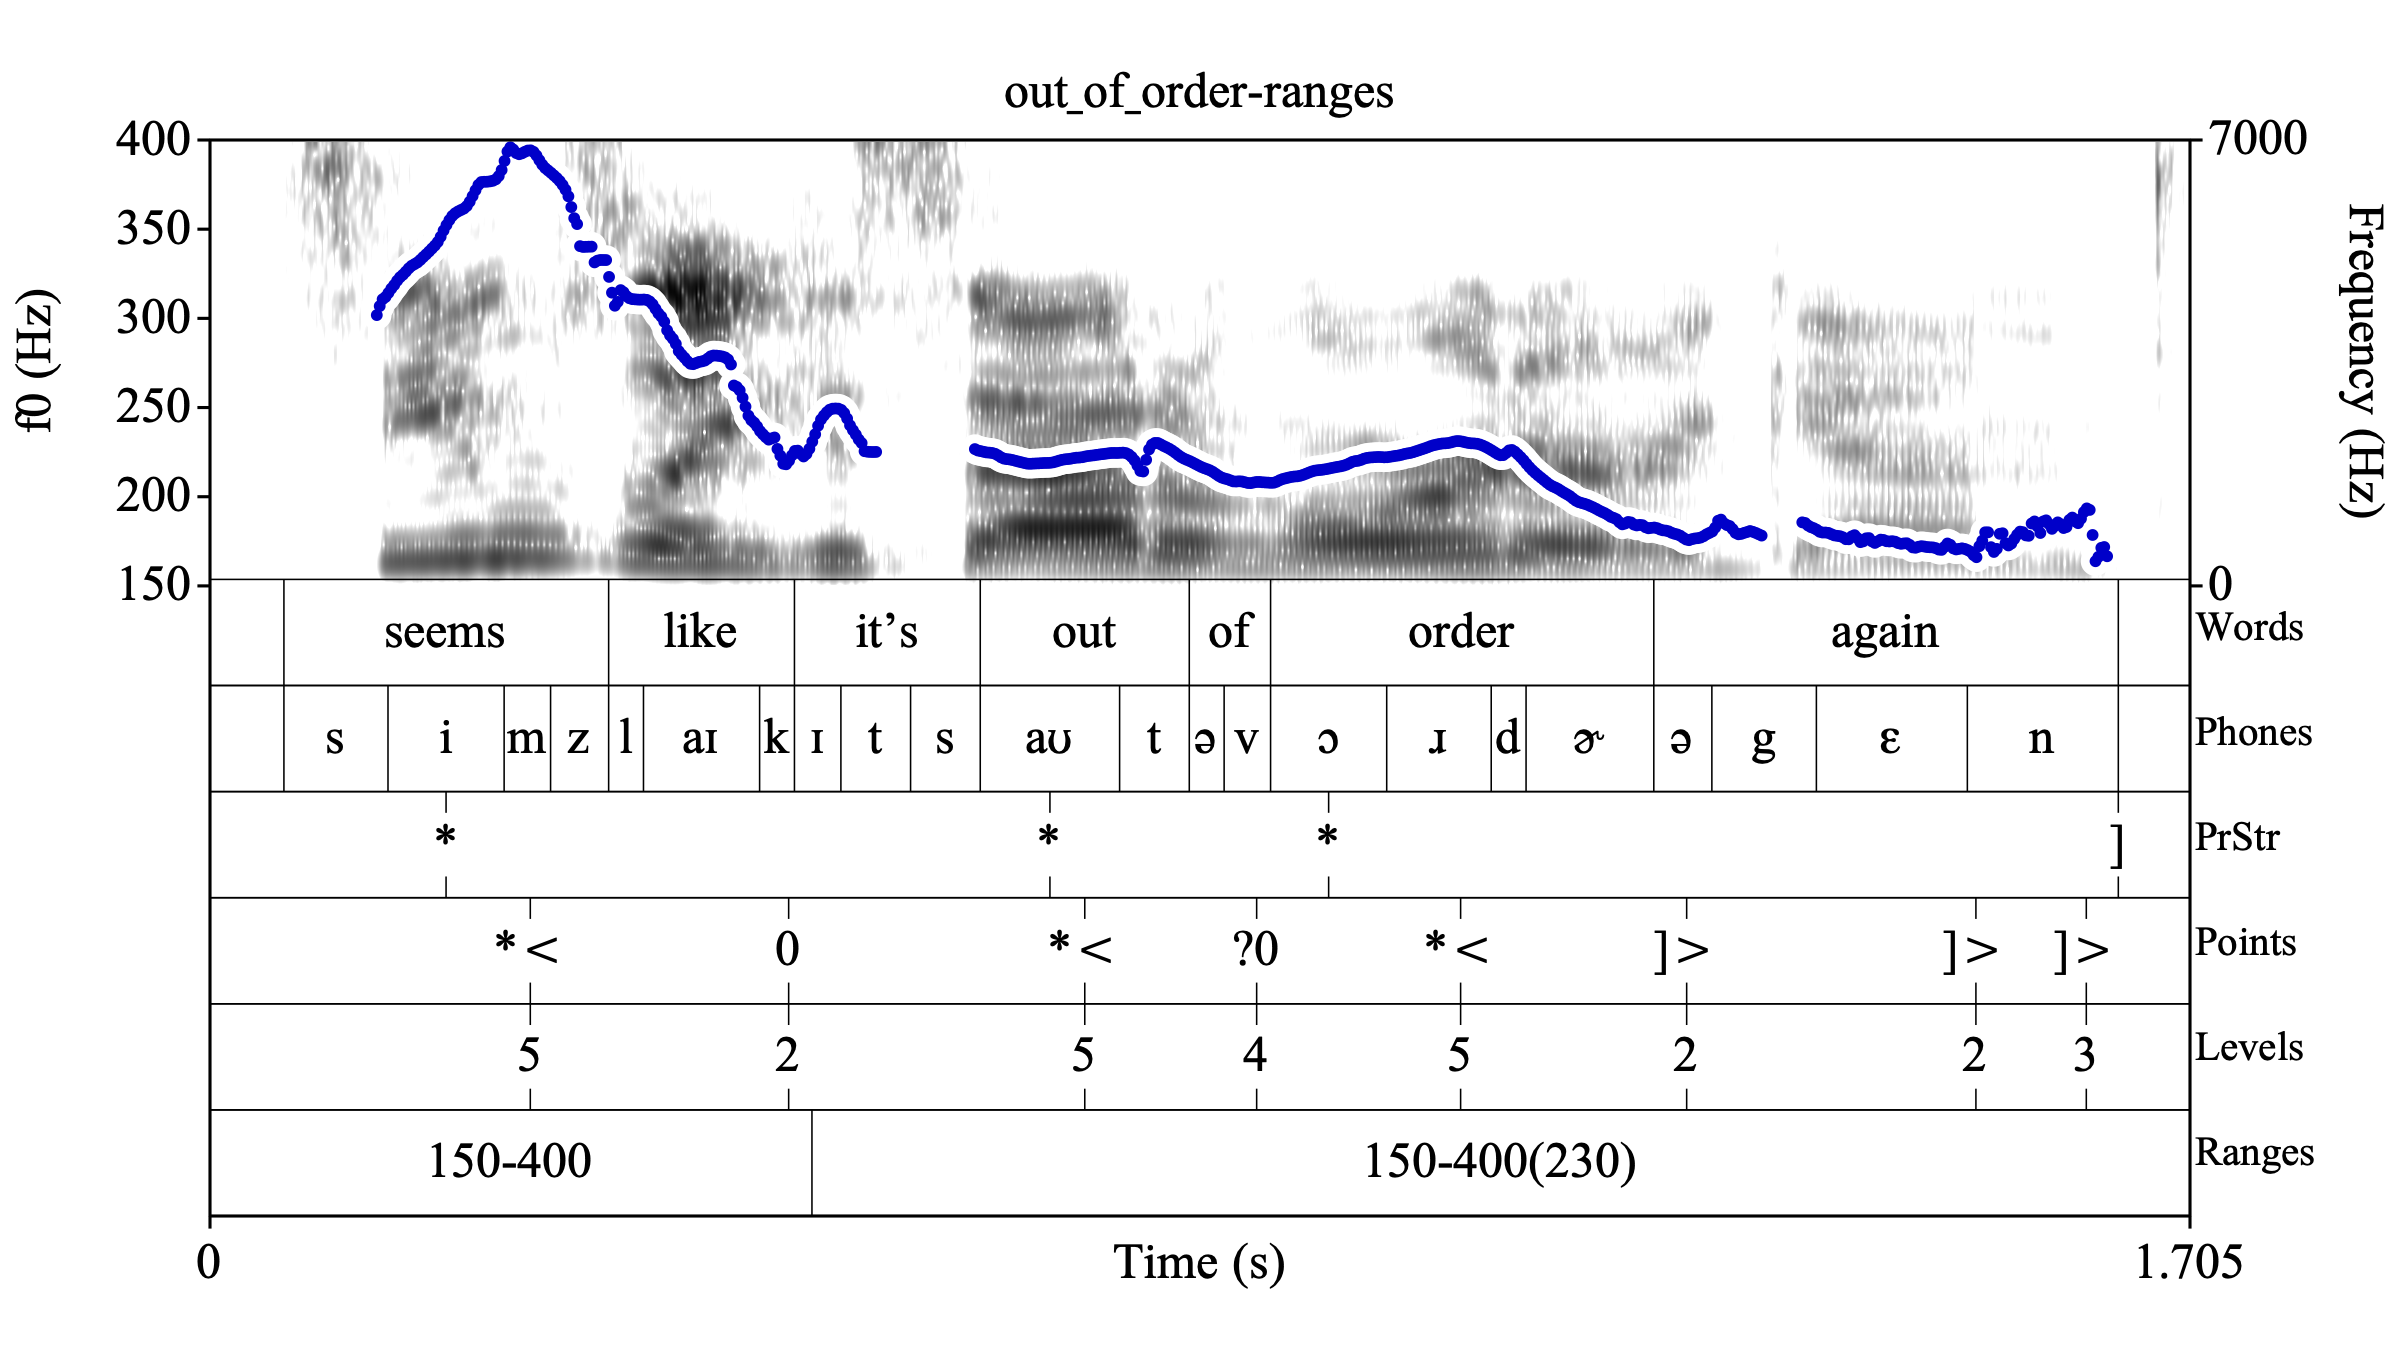
\includegraphics[width=.875\linewidth]{Ranges-out_of_order-ranges-2RangeIntervals.png}
%
\caption{One prosodic phrase (PrStr annotation) and two local pitch ranges (Ranges annotation).%
\label{fig:out_of_order-ranges Ranges Adv}%
\index{Annotated example, Ranges tier (advanced)!out\_of\_order-ranges}
}
\end{figure}

Here, \langtext{seems like} occurs in a pitch range with a much higher f0 maximum than \langtext{it’s out of order again}, but the labeller also perceives \langtext{out} and \langtext{order} as high pitched. Though the pitch range changes after \langtext{seems like}, the labeller does not perceive enough of the cues to disjuncture (e.g., pauses, final lengthening, initial strengthening, etc.) for them to label different prosodic phrases on the PrStr tier. As such, the labeller does not annotate a \textlabel{]} between \langtext{like} and \langtext{it’s}, but does annotate a new Ranges boundary with a lower ceiling, to indicate that they hear \langtext{out} and \langtext{order} as high accents.

In this way, though some analyses would treat this drop in the pitch ceiling as due to the presence of certain phonological objects (e.g., a “downstep accent”), PoLaR treats all pitch range compression the same — with a new Range interval. In other words, the time-alignment of Range intervals is independent of prosodic phrase boundaries.

Thus, the main characterization of the range compression in this “downstep” context is the beginning of a new Range interval, the beginning of which is time-aligned to be where the pitch ceiling has finished falling. Another example exhibiting range compression is given in Figure \ref{fig:economy Ranges Adv}, where there are two successive instances of range compression, and where the timing of the Range intervals is instructive.

\begin{figure}[H]
\centering
%
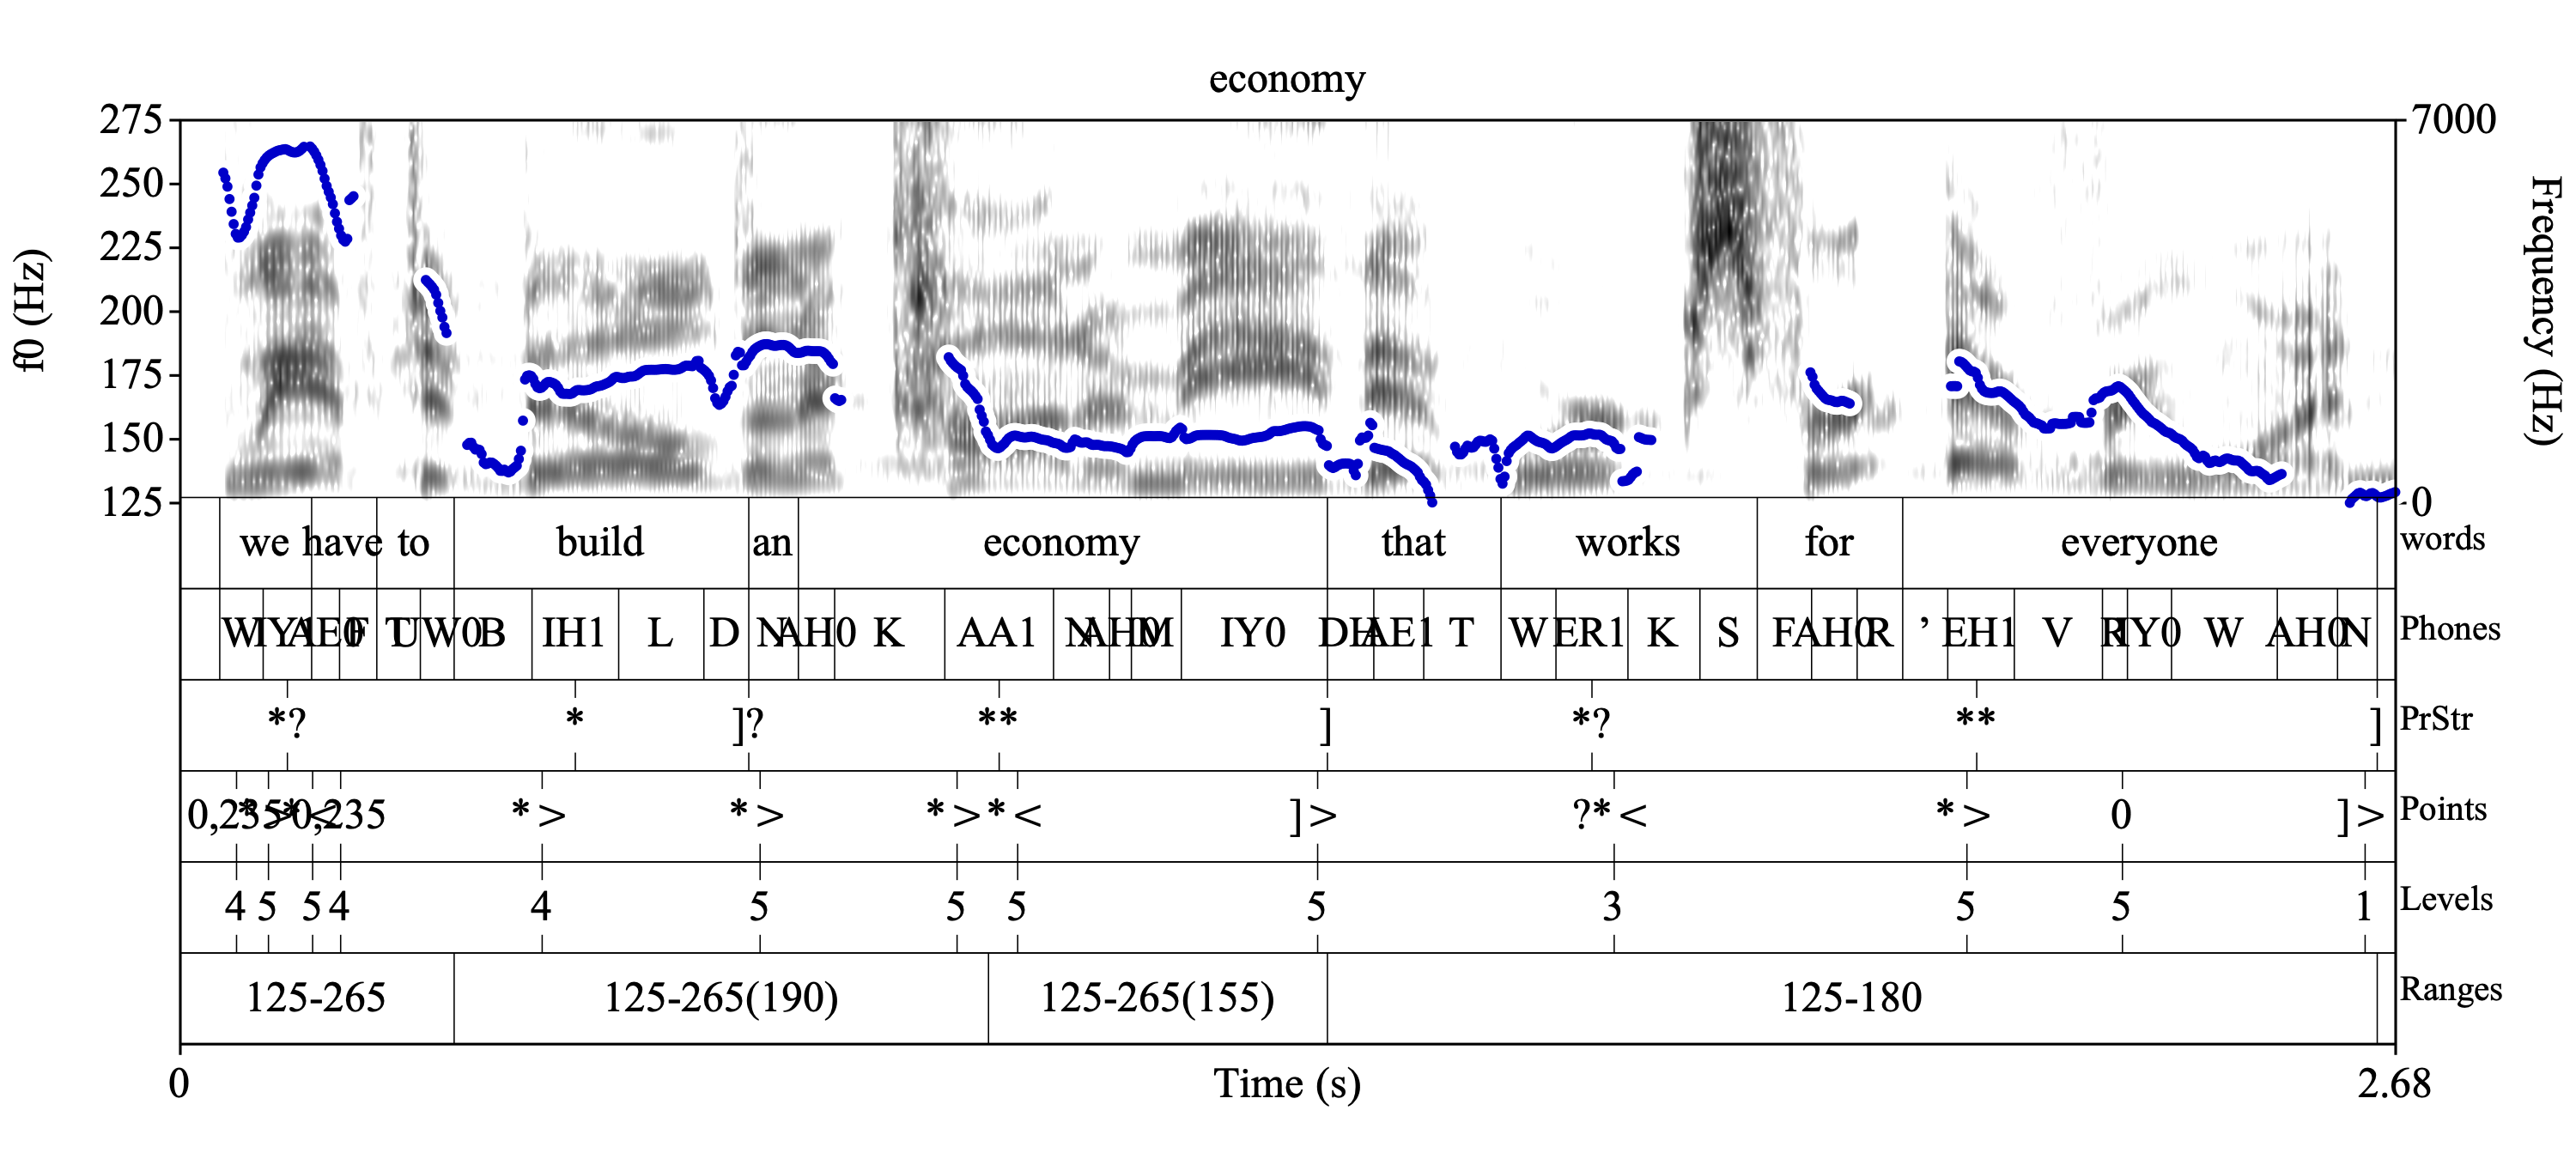
\includegraphics[width=.875\linewidth]{Ranges-economy-advanced.png}
%
\caption{Multiple Ranges intervals, where the labeller’s analysis includes multiple instances of range compression.%
\label{fig:economy Ranges Adv}%
\index{Annotated example, Ranges tier (advanced)!economy}
}
\end{figure}

In this example, the string \langtext{we have to build an economy} consists of a single prosodic phrase, and a novice labeller may label this entire phrase as a single Range interval of 125-265. A more advanced labeller (especially one trained to look out for downstepping) would notice that the pitch range is compressed twice, to account for the interpretation that \langtext{we}, \langtext{build}, and \langtext{economy} are all prominent and have high accents. The pitch ceiling falls from around 265Hz during \langtext{we} to about 190Hz during \langtext{build an}; the ceiling then falls again to around 155Hz in \langtext{economy}. What’s especially instructive here is the timing of the pitch ceiling’s fall during \langtext{economy} (which ToBI labellers may recognize as a \textlabel{H+!H*}): the pitch ceiling is dropping \textit{during} the [a] vowel, and reaches the end of its fall about one third of the way into it. Since the Ranges interval labels track the pitch floor and the pitch ceiling, the new Range should begin where the change in range is completed; i.e., where the pitch ceiling’s fall is completed. (Note that after \langtext{economy}, there is a new Range interval, whose beginning is time-aligned to the start of a new prosodic phrase. While ranges and phrases are independent, phrase boundaries do frequently coincide with new Ranges intervals, since phrase boundaries may trigger a pitch reset; for recent work on the coincidence of pitch reset and phrase boundaries, see \citealt{brugos15} and \citealt{kim20}.)

While the guidance is relatively clear in these cases of compression, Ranges interval labellers may at times find it challenging to determine how many range changes are appropriate, after several instances of compression, when the speaker’s local range(s) gets very narrow. In such cases of ambiguity, as with Points tier labelling, we recommend erring on the side of over-labelling, and putting in more Ranges intervals rather than fewer.

It should also be noted that, while the labels in Figure \ref{fig:economy Ranges Adv} indicate an analysis that there are two instances of range compression (indicated by the usage of two subranges), this is an \emph{analytical choice}, and equally valid (but analytically different) labels might not include one or both of these compressions. For example, under a different analysis, a labeller may treat the f0 fall during “\langtext{economy}” as a fall-to-low – if so, “\langtext{an economy}” should fall within the same interval on the Ranges tier. To be clear, this means that (like other Advanced PoLaR labels), different analyses can be tracked by using different Advanced Ranges labels. (PoLaR does not force any analytical choice; the usefulness of PoLaR is that it can keep track of whatever analysis the labeller prefers.)

\subsubsection{Expanded ranges: when a range is compressed relative to what follows}\label{sec:expanded-ranges-when-a-range-is-compressed-relative-to-what-follows}

Another type of local range change, one parallel to range compression as discussed above, is where subsequent prominences are realized with relatively higher pitch, which is sometimes referred to as “upstep.” PoLaR annotation can capture such pitch relations via the range tier in analogous ways to range compression relative to earlier highs.

The example another-little-banana shows such a case. Here, two prominences on \langtext{another} and \langtext{little} are both realized with high-sounding pitch, but the second prominence is noticeably higher. The labeller has captured that the f0 is high on both \langtext{another} and \langtext{little} by labelling two ranges, the first with a maximum of 245 Hz, and the second with a higher maximum of 330 Hz. (Note that these ranges are both within the domain of a single phrase in the PrStr tier.) Here, the Advanced ranges labelling captures the pitch expansion by means of labelling a lower ceiling in parentheses in the first range, reflecting that a Basic Ranges tier label would capture only one range with the higher ceiling for the whole utterance.

\begin{figure}[H]
\centering
%
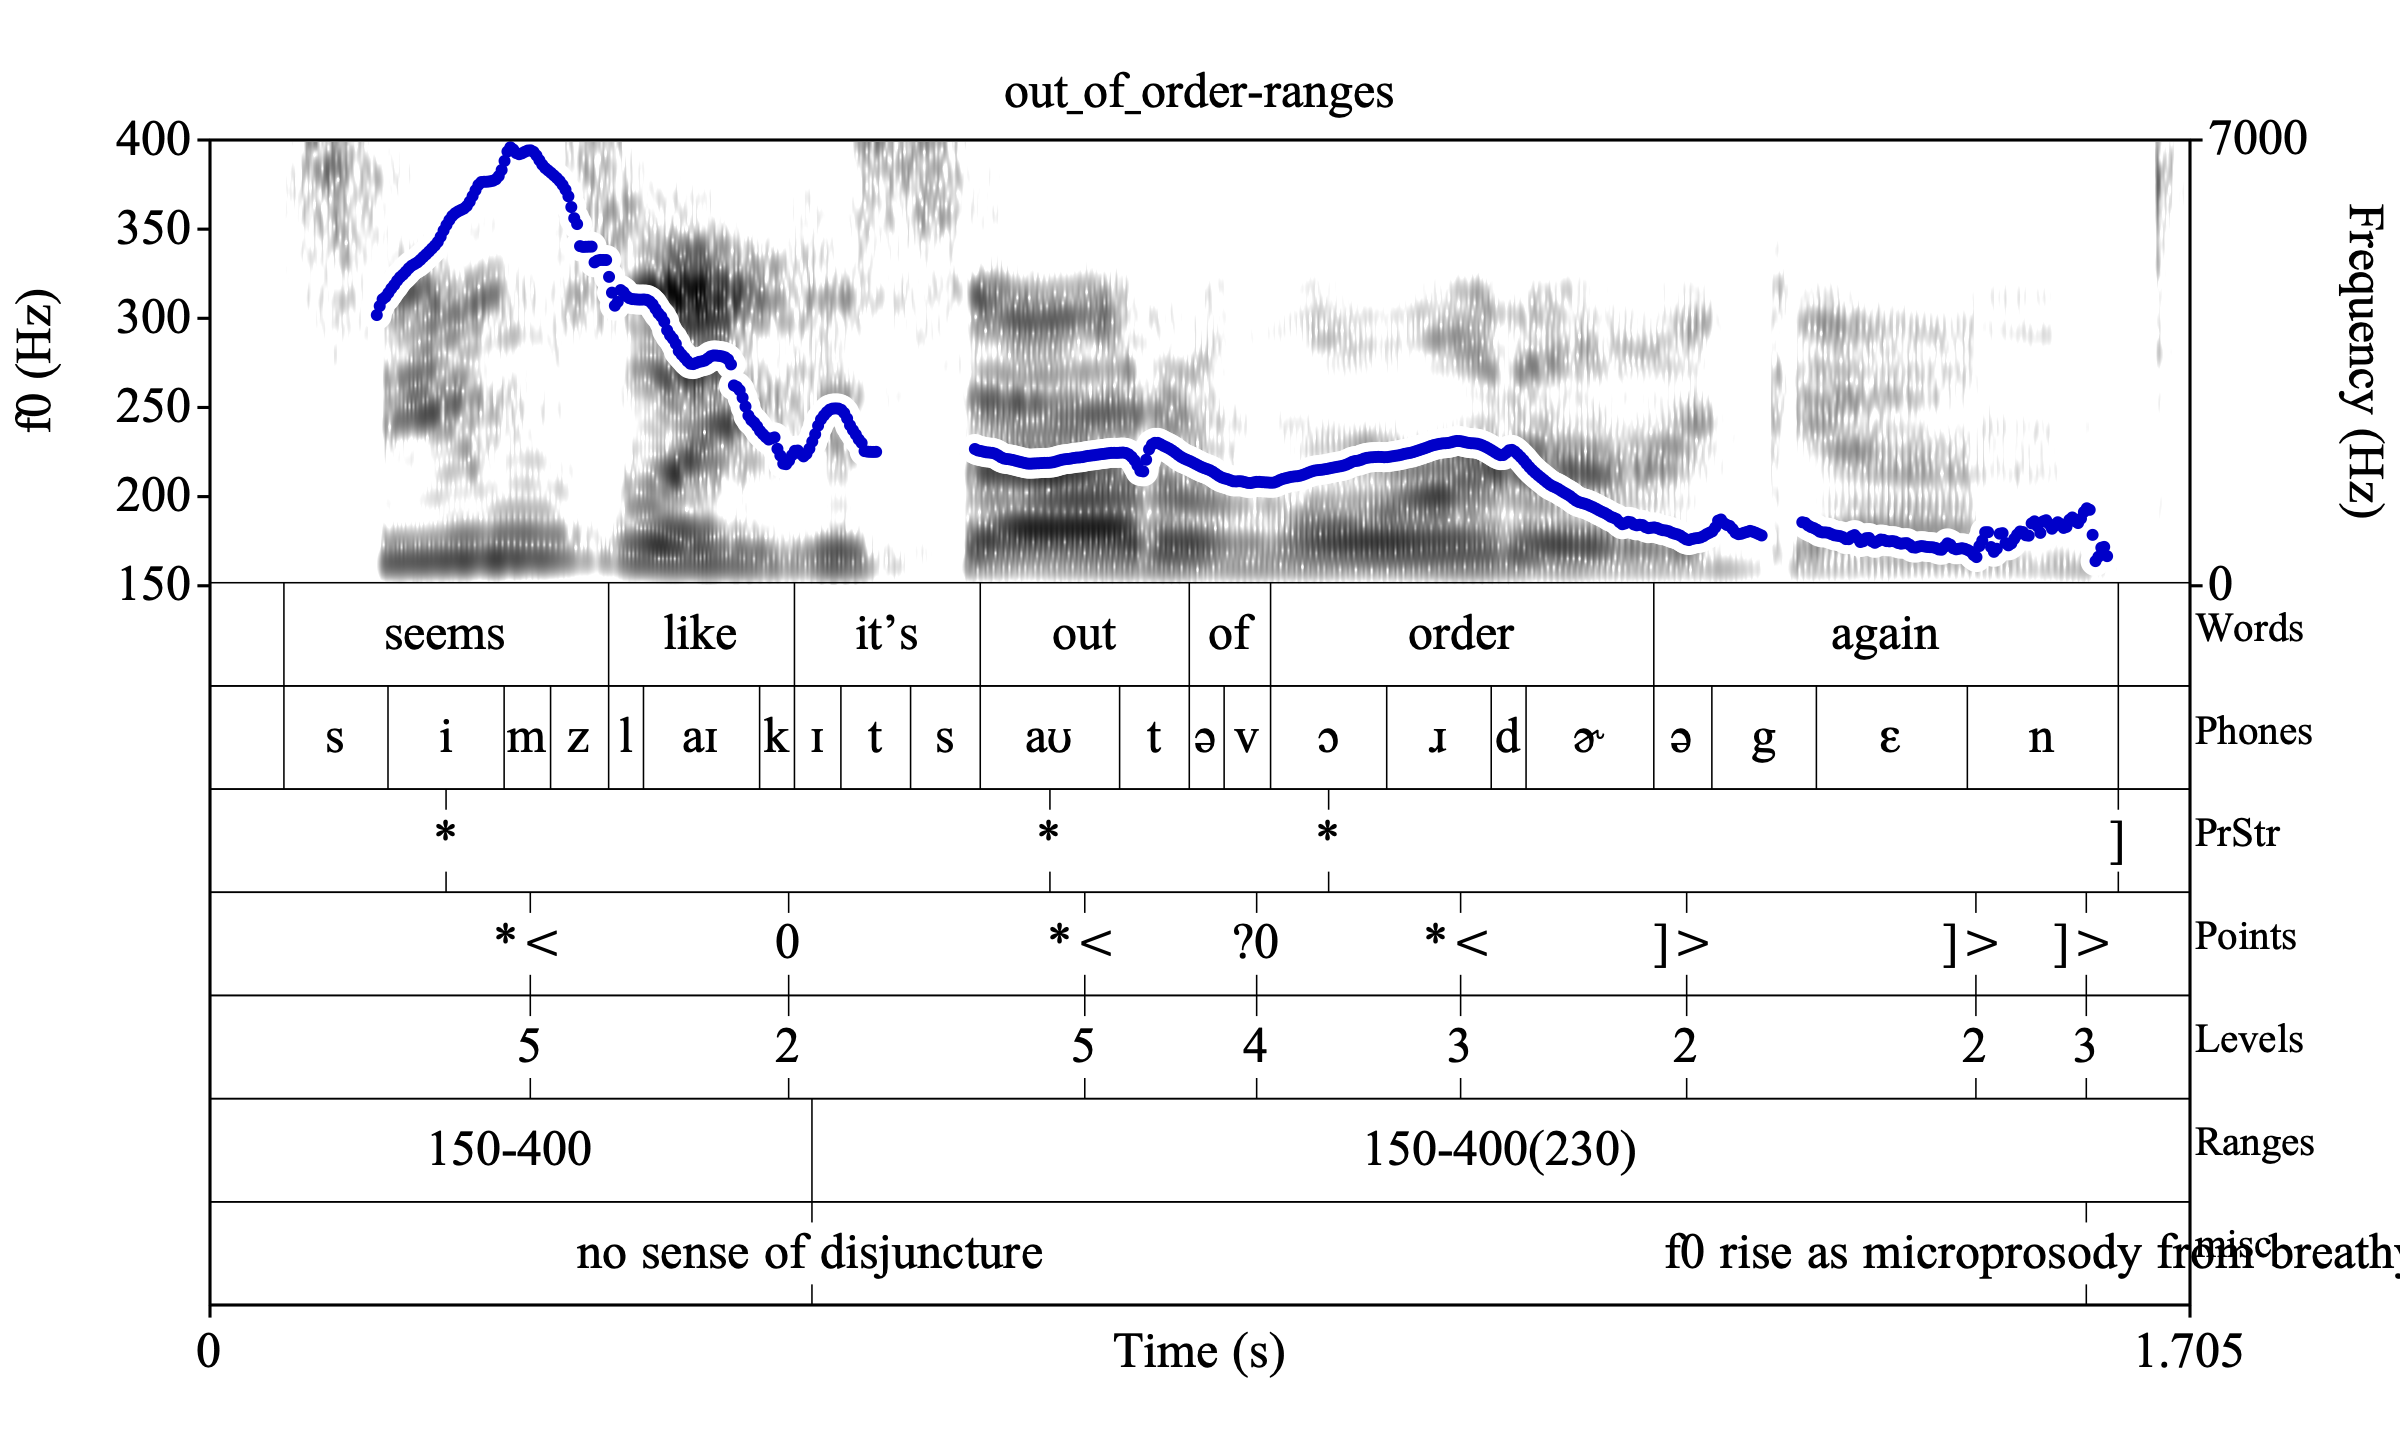
\includegraphics[width=.875\linewidth]{Ranges-another-little-banana-adv.png}
%
\caption{\texttt{another-little-banana}, with Advanced PoLaR labels.%
\label{fig:another-little-banana Ranges Adv}%
\index{Annotated example, Ranges tier (advanced)!another-little-banana}
}
\end{figure}

Ultimately the motivation for these two range intervals here is to indicate that the labeller hears the pitch movement in \langtext{another} to be rising from low to high – and the Range tier annotations indicate the pitch floors and pitch ceilings. If only a single ranger were used, the Levels labels for \langtext{another} would not be 1-5, but 1-3 — and the 1-3 rise might not accord with the labeller’s intuition that the pitch during \langtext{another} reaches a “high”. This follows from the general idea that what Levels labels indicate is where “high” and “low” are (with the assumption that “high” corresponds to 4 or 5, and low “1” or “2”).

\subsubsection{A few examples of range changes signalling parentheticals }\label{sec:a-few-examples-of-range-changes-signalling-parentheticals}

As mentioned in the section above on the relative stability of the pitch floor, there will be cases where both floor and ceiling change across ranges. One such example of this was already shown in the introduction to the Ranges tier in the Basic labels chapter, and is repeated here – note that this is not a parenthetical, but exemplifies a similar intonational phenomenon. In the third range of the example advice-falsetto-NPR, the speaker has shifted the top of her range up to 750 Hz, and also shifted her local lows to a relatively high 250 Hz. In this example, the ranges shift at the locations of the phrase boundaries, as marked in the PrStr tier.

\begin{figure}[H]
\centering
%
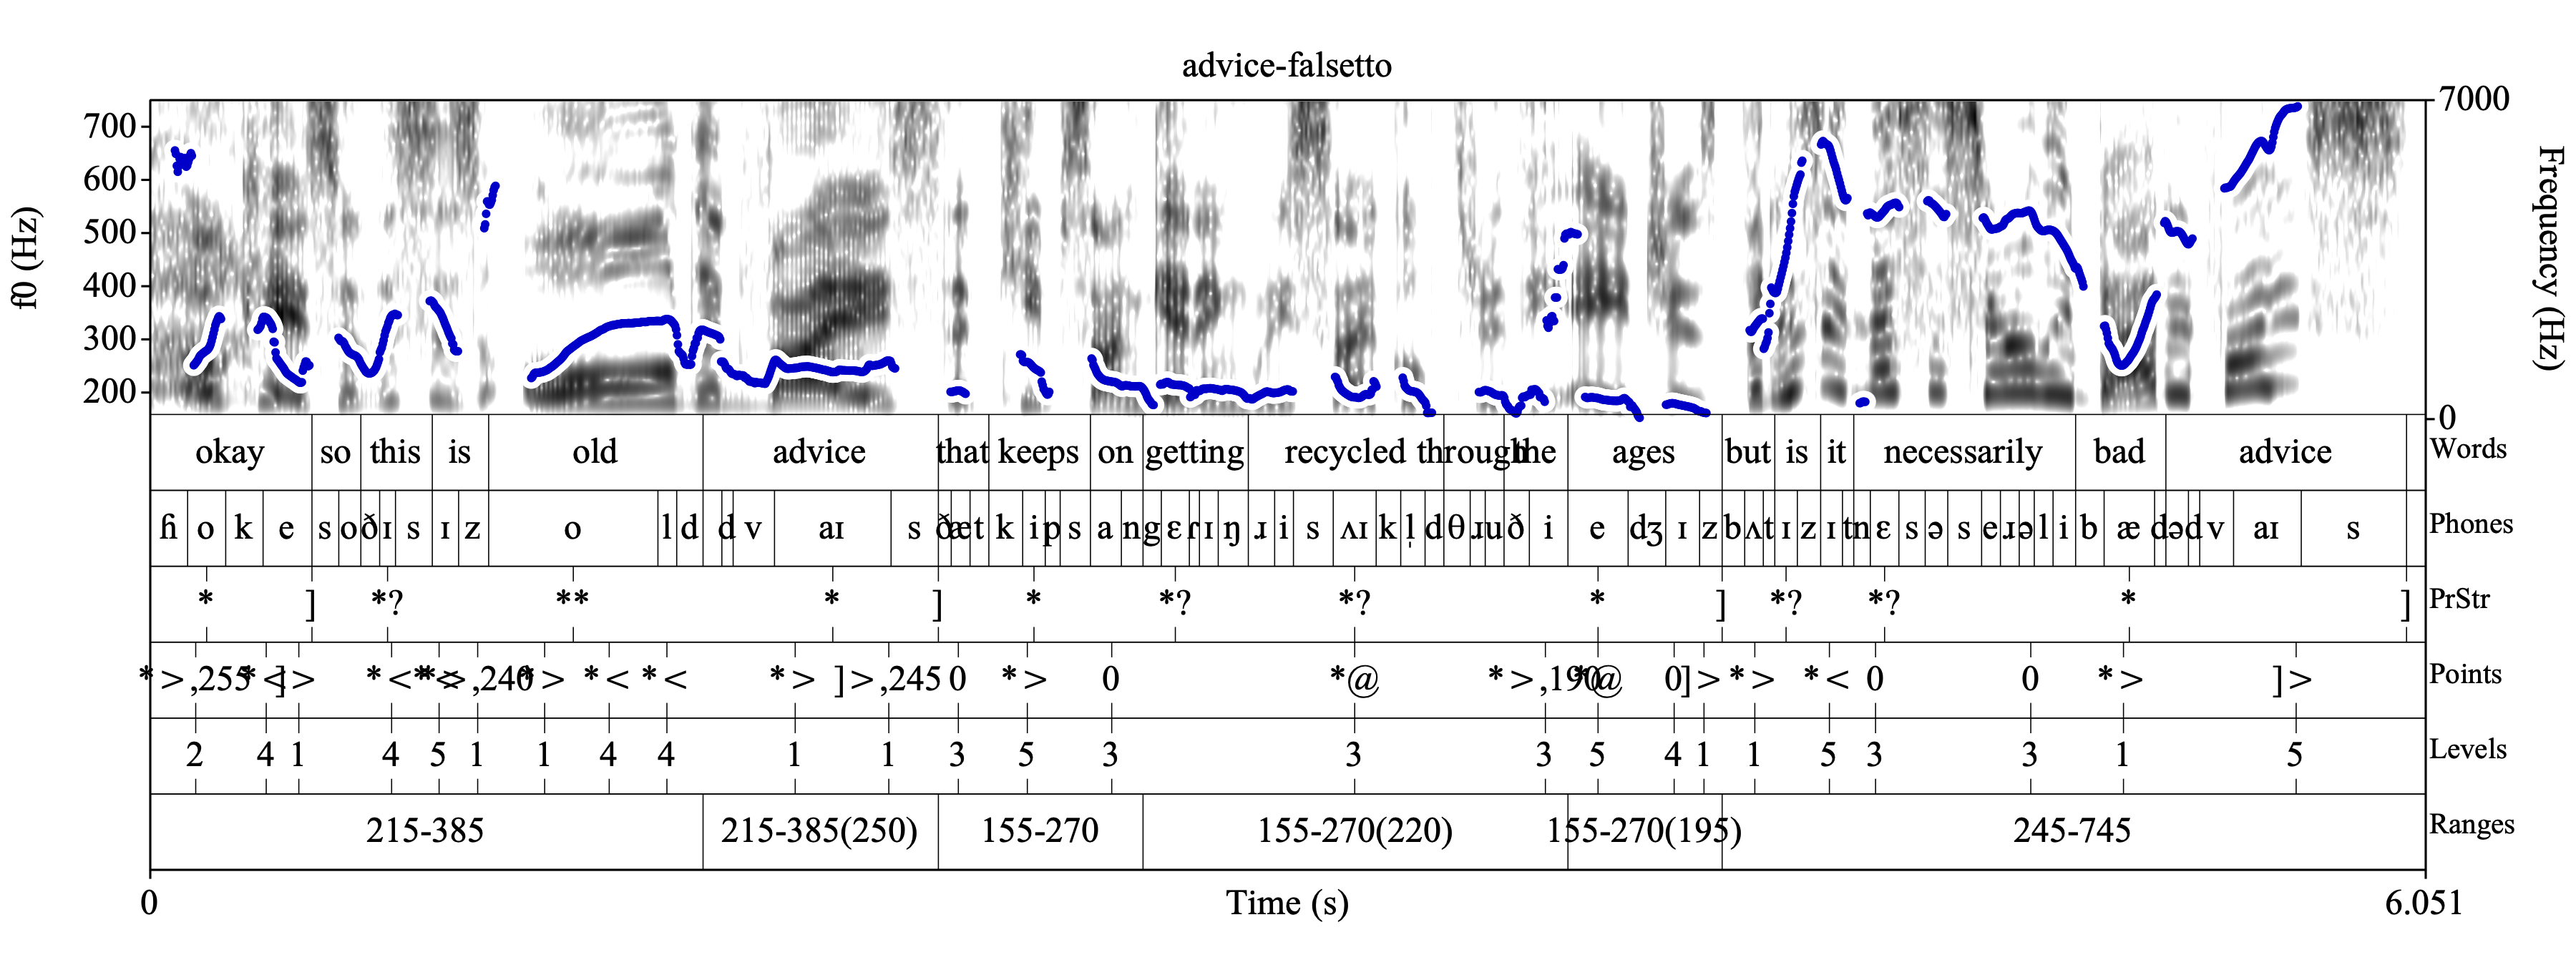
\includegraphics[width=\linewidth]{Ranges-advice-falsetto-advanced.png}
%
\caption{An example of both the pitch floor and ceiling of a range shifted upward.%
\label{fig:advice-falsetto Ranges Adv}%
\index{Annotated example, Ranges tier (advanced)!advice-falsetto}
}
\end{figure}

Parentheticals are often signalled via a different pitch range – commonly one that is lowered. The example below shows such a case, where the parenthetical phrase (“\langtext{who never listens}”), is produced in a pitch range (130-180Hz) that has both a lower ceiling than the preceding and following phrases, and also a more compressed range (only a 50Hz span compared to the neighboring ranges, which each span over 100Hz.) Here, the range domains correspond to the phrasing, as indicated in the PrStr tier.

\begin{figure}[H]
\centering
%
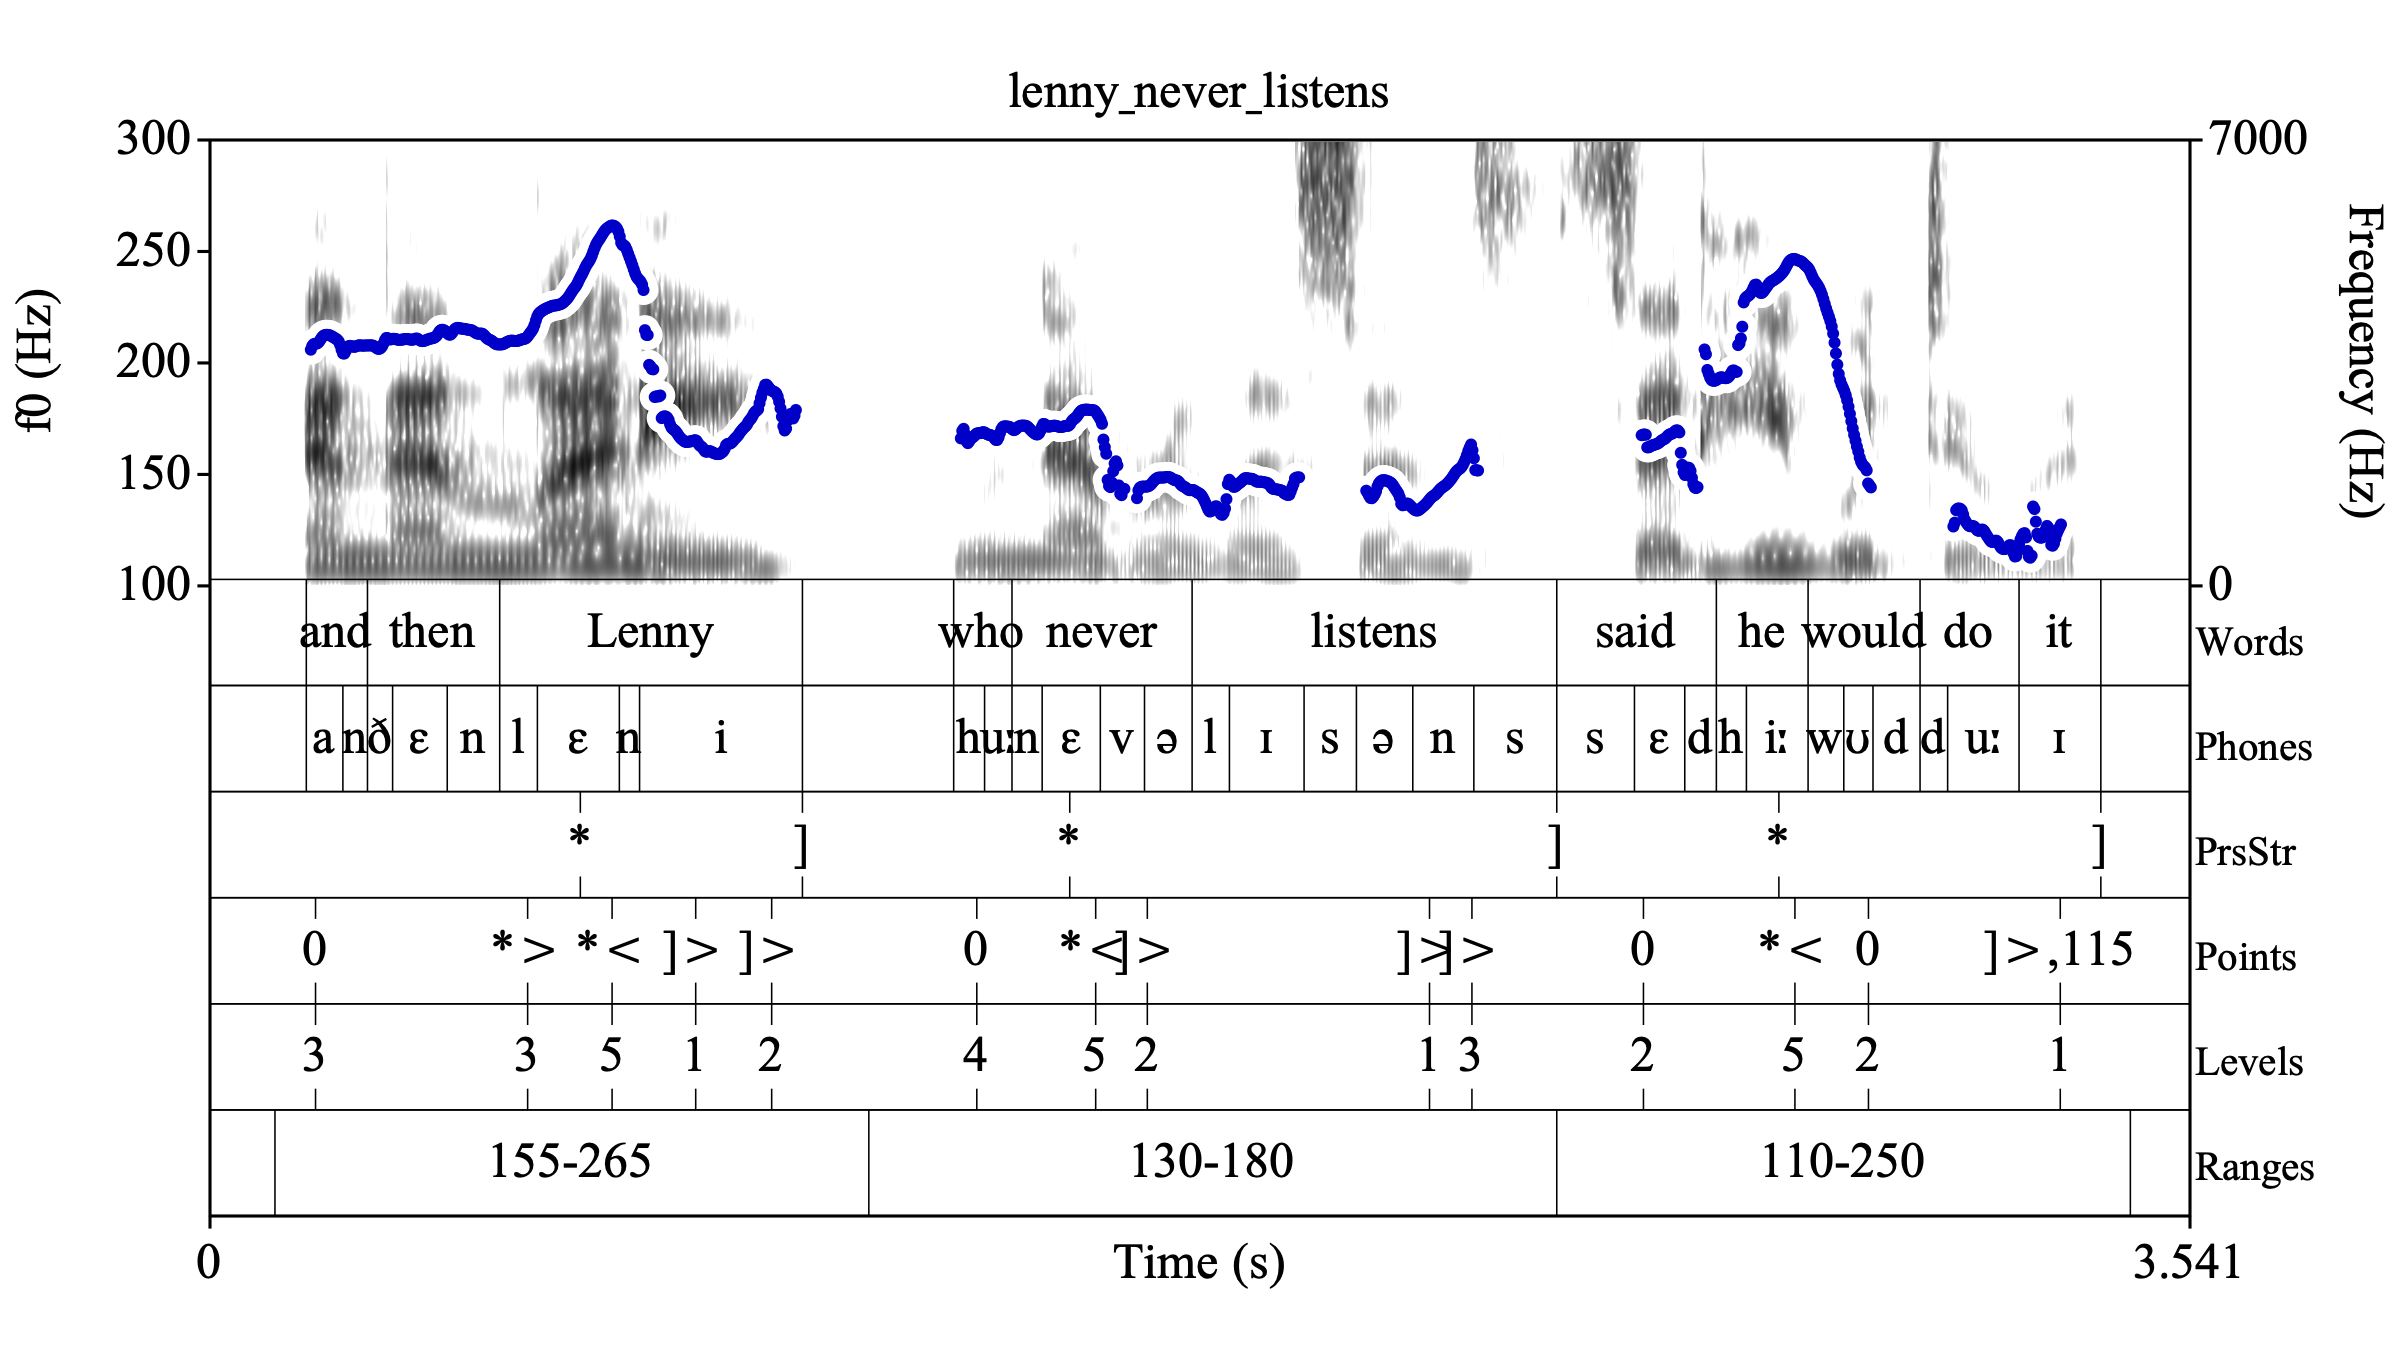
\includegraphics[width=.875\linewidth]{Ranges-lenny_never_listens-adv.png}
%
\caption{An example of a compressed parenthetical.%
\label{fig:lenny_never_listens Ranges Adv}%
\index{Annotated example, Ranges tier (advanced)!lenny\_never\_listens}
}
\end{figure}

The following pair of examples illustrate that range changes signalling a parenthetical need not necessarily be accompanied by phrase boundaries in the PrStr tier. In the first example, the word \langtext{honestly} is produced in an expanded range compared to the preceding and following speech. And in the second text, the converse happens, with \langtext{honestly} produced in a compressed range compared to the preceding and following parts of the utterance. In these examples, there are similar ranges on either side of the parenthetical word. Labelling the ranges for this type of example may be useful for researchers investigating the role of pitch in perceptual grouping, including non-local and global pitch relations (see, e.g., \citealt{ladd88}, \citealt{geluykensswerts93, geluykensswerts94}, \citealt{brugos09}, and \citealt{kentnerfery13}).%\citealt{petrone10}, 
%todo not sure why petrone10 is commented out

\begin{figure}[H]
\centering
%
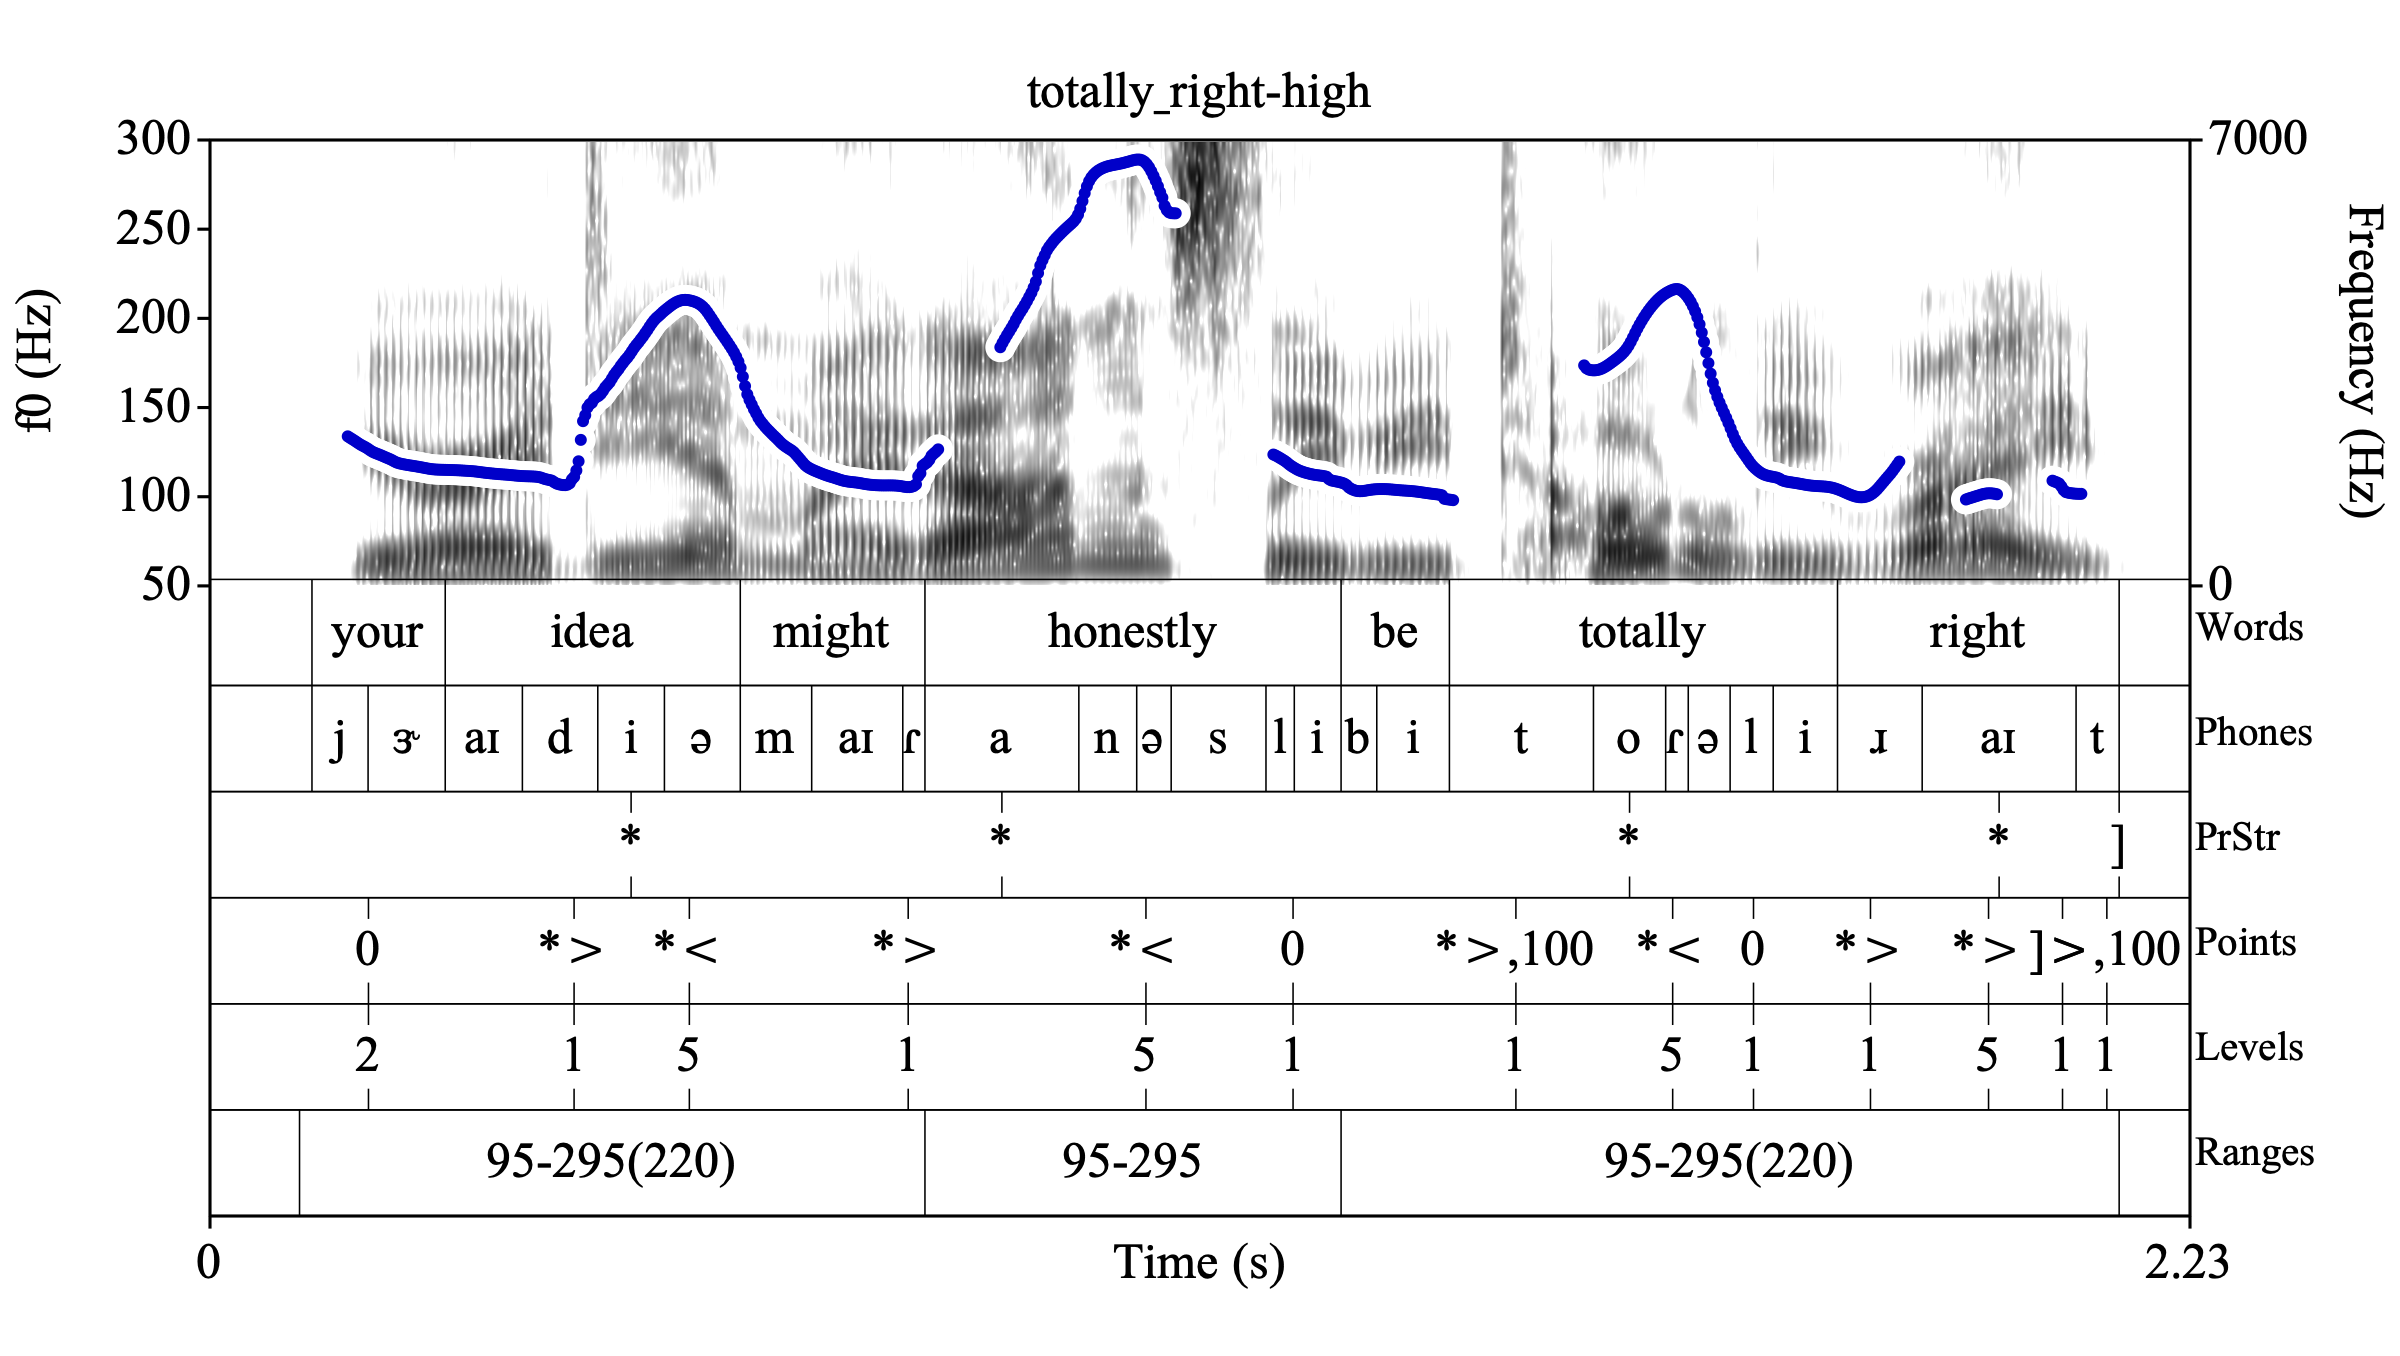
\includegraphics[width=.875\linewidth]{Ranges-totally_right-high-advanced.png}
%
\caption{An example of a locally expanded range.%
\label{fig:totally_right-high Ranges Adv}%
\index{Annotated example, Ranges tier (advanced)!totally\_right-high}
}
\end{figure}

\begin{figure}[H]
\centering
%
\includegraphics[width=.875\linewidth]{Ranges-totally_right-low-advanced.png}
%
\caption{An example of a locally compressed range.%
\label{fig:totally_right-low Ranges Adv}%
\index{Annotated example, Ranges tier (advanced)!totally\_right-low}
}
\end{figure}

\subsection{How ToBI and PoLaR treat Ranges}\label{sec:how-tobi-and-polar-treat-ranges}
A knotty issue in intonation labelling is how to deal with changes in a speaker’s local ‘operational range’, both within and across utterances.  This issue is critical, because it has profound implications for what counts as a High vs a Low intonational target.  If you are familiar with the ToBI system, you will recognize that ToBI addresses the question of local pitch range (and changes in that range) in several ways that do not involve explicitly labelling range information. We review some of these mechanisms in the following paragraphs, and compare them with PoLaR’s approach to labelling changes in local pitch ranges (e.g., compression).  In a following section we turn to PoLaR’s approach to determining the intonational target scaled pitch level within a speaker’s current ‘operational pitch range’. (We are comparing and contrasting PoLaR with the ToBI annotation framework, given ToBI’s widespread familiarity among intonationists. Note that several of the points made with respect to ToBI can be extended to other categorical\slash phonological annotation systems. Readers who are not interested in the relationship of ToBI to the PoLaR system may prefer to skip the present section.)

Since its inception, the phonologically-based ToBI system for annotating intonational prosody (cf. \citealt{beckman-05}) has not been concerned with range changes, and intentionally has not provided tools for annotating ranges.  This decision was motivated by a theoretical stance: the same phonological contour can be realized in different ranges, and the choice of range is assumed not to be a phonological distinction.  However, in the years since ToBI was developed, extensive experience with intonational labelling has suggested that range changes may play a different and perhaps more important role than was originally assumed.  As a result, PoLaR includes conventions for explicitly labelling the speaker’s local f0 range, as it changes both within and between utterances. Here we discuss the phenomena of downstepping (compression where the pitch ceiling drops), upstepping (expansion where the ceiling rises), range shift (where both floor and ceiling move), and range ambiguity, which are handled differently in ToBI and PoLaR annotation, due to the differences in the goals of the two systems.

As a reminder, ToBI and PoLaR are mutually supplementary annotation systems, with different goals, which can be used in concert.  PoLaR is, in a sense, a response to and an embodiment of insights acquired by many ToBI labellers over three decades of experience, which has (not surprisingly) identified a number of challenges in intonational labelling. We envision that the two approaches will be able to inform each other not only about the range of possible phonetic realizations of a given phonological specification of a tonal contour, but also about the possibility of identifying contrastive tonal phenomena not available for annotation in the ToBI system. PoLaR 1.0 represents our current proposal for the form that such a complementary acoustic-phonetic labelling system might take; feedback from users is actively sought and will be very welcome.

\subsubsection{How ToBI and PoLaR handle downstepping}\label{sec:downstepping-am-models-and-tobi-annotation}
In our experience, the task of determining the local Range that a speaker is currently using, within his or her overall f0 range, is generally a reasonable one, although specific instances can be challenging. One such challenge arises because, in a sequence of High tonal targets, later High targets are frequently realized with a lower f0 than a preceding High target. There are two commonly distinguished sources for this phenomenon. The first is phonetic declination: the gradual lowering of the top of the speaker’s f0 range (i.e., the f0 ceiling) over the course of speech. The second is perceived as contrastive (and thus arguably phonological), because the range drops steeply and suddenly. Thus intonational annotation systems are faced with a question of which examples (if any) of this type of event to annotate and (if so) how.

MAE\_ToBI addresses this issue by making use of a diacritic only in situations of downstep (using the \textlabel{!} diacritic before the relevant \textlabel{H} symbol), and does not mark downdrift at all. Moreover, the usage of the downstep diacritic is treated by ToBI as grammatically constrained: it can only be used when the previous High tone within the same intonational constituent of the relevant sort. In the current AM model (cf. \citealt[17–18]{beckman-05}, and references therein), the domain of downstep is the intermediate phrase, and the downstep label indicates that the pitch ceiling is lowered for the remainder of that intermediate phrase, specifying a narrower range. This grammatical analysis is beneficial in that it makes testable predictions, however it is not ideal for ease of labelling: it requires that labellers be trained to keep enough of the intonational model in working memory so as to be able to identify downstep only in such contexts while labelling. Moreover, it only allows labellers to keep track of certain types of range changes: only those that adhere to the grammatical definition of downstep.

In contrast, PoLaR Ranges are not subject to such constraints: in the PoLaR system, ranges can be annotated independently of the presumed phonological constituent structure of the utterance. As a result, what MAE\_ToBI regards as downstep (restricted to the ip domain) can in PoLaR be labelled in stretches of speech of any length or constituent structure, and even downdrift can be annotated with a different Ranges interval, if the labeller finds it to be a significant enough change over time. From a theoretical\slash analytical standpoint, this is useful for capturing cases where what appears to be downstep occurs across a phrase boundary, i.e. cross-phrase pitch range relations (cf. \citealt{ladd88, brugos15}), which are not possible to annotate while adhering to the grammar of MAE\_ToBI. From a practical standpoint, this is also beneficial in that labellers need not reference a grammar to decide when to track pitch compression by adding a new Ranges interval.

\subsubsection{How ToBI and PoLaR handle upstepping}\label{sec:upstepping}
A less common but still frequently-occurring phenomenon in American English intonation occurs when a High prominence is followed by another High with a higher f0 peak.  This phenomenon can be thought of as upstepping. In MAE\_ToBI, at least, there is not a standard way to capture such a range relation.  That is, a sequence labelled \textlabel{H* H*} can be used in three different situations: when two successive High prominences are realized with approximately equal pitch height, when the second High is realized with a lower pitch that can be attributed to declination (as discussed above), or when the second High is noticeably higher. These possibilities cannot be distinguished in MAE\_ToBI, which is appropriate if they do not signal a phonological contrast. Nevertheless, it might be of considerable interest to know where they occur. ToBI systems developed for some other languages have implemented ways of capturing upstep; see, for example the discussion in \citet{armstrong-14} of the use of the \textlabel{¡} diacritic (inverted exclamation point) for annotation of varieties of Spanish and Portuguese. PoLaR takes a different approach to upstep, just as for downstep: such cases can be handled by annotating the beginning of a new and wider Range, to permit a distinction between upstepped and non-upstepped sequences.
%todo this paragraph is commented out… revisit
%Cases in which a High prominence is followed by another High with a higher f0 peak are widely observed by labellers; this phenomenon can be thought of as upstepping. In MAE\_ToBI, at least, there is not a standardized way to capture such a range relation. That is, a sequence labelled \textlabel{H* H*} can be used for two successive High prominences with different scaling relationships: they can be either of approximately equal pitch height, or the second High can be noticeably higher, and these two possibilities cannot be distinguished. Some other ToBI systems have implemented ways of capturing upstep; see, for example the discussion in \citealt{armstrong-14} of the use of the \textlabel{¡} diacritic (inverted exclamation point) for annotation of varieties of Spanish and Portuguese. In PoLaR, such cases can be handled by annotating a new and wider Range, opening the possibility of distinguishing between upstepped and non-upstepped sequences.

\subsubsection{Range-labelling challenges addressed by PoLaR}\label{sec:range-labelling-challenges}
Because range changes and phrase boundaries are tightly linked in the ToBI framework, some types of attested data are challenging to label.  These problems include:

\noindent1) \uline{Range changes force annotation of a phrase break}: When there is a big jump in range, either up or down, ToBI requires a phrase break, even if there is no other sense of disjuncture.\footnote{An exception is made for cases where a disfluency is followed by the beginning of a new phrase before the disfluent phrase was completed, in which case the annotation \%r (for ‘reset’) is used}

Because PoLaR allows the labeller indicate a range change within a phrase (or even within a word, as in Figure \ref{fig:economy Ranges Adv}), it provides a tool for capturing within-phrase changes in f0 range when they occur. 

\noindent2) \uline{Range changes prohibit annotation of a phrase break}: In some cases there is a conflict between downstepping evidence that requires two targets to be in the same phrase, and other acoustic evidence that requires them to be in different phrases, because it suggests the presence of a boundary between them. ToBI labellers sometimes address this conflict by using the Break Indices \textlabel{3-} or \textlabel{2}, indicating conflicting evidence for the boundary, but in general the ToBI prohibition against downstepping across ip’s means that if you want to keep track of perceived downstepping, you may need to violate your sense of phrasing.

Because PoLaR is agnostic about the theory-based constraint against downstepping across phrases, range change annotation is de-linked from the phrase\slash prominence annotation. Phrasal structure and prominence location are labelled in the PrStr tier, while Range is annotated in its own tier, so that a new Range can begin anywhere in an utterance.

\noindent3) \uline{Ambiguity between H and L targets}:  There are circumstances in which it is clear that a tonal target for a boundary or a prominence has occurred, but it difficult to determine whether that target is a H or a L tone.  ToBI labellers are familiar with the uncertainty\slash ambiguity that arises when a pitch accent in a very compressed low range, often at the end of a phrase, might be a Low (\textlabel{L*}) or a downstepped High (\textlabel{!H*}).  Similarly, sometimes an \textlabel{L*+H} label is required for a pitch accent even though the \textlabel{L*} accented syllable is realized with a higher f0 than the preceding syllable.  PoLaR does not explicitly distinguish between H and L target tones, but rather uses the Range annotation and f0 values to determine which of 5 levels each target is realized with.  As a result, it does not require labellers to make a phonological decision about H vs L, but instead provides the option of noting the compressed (or expanded) pitch range.

In sum, PoLaR provides a tool to address some of the challenges and ambiguities associated with labelling f0 range change phenomena that are always easy to deal with in more-phonologically-based approaches like ToBI.  To the extent that these range changes are systematically controlled by speakers and attended to by listeners for communicative purposes, PoLaR’s capacity to capture them may provide a useful supplement to phonological labels, as a means to systematically keep track of where pitch range is manipulated.

\section{Levels (Advanced)}\label{sec:levels-advanced}
In PoLaR’s present instantiation, the Levels are automatically determined by an algorithm, based on the hand-annotations in the Ranges and Points tiers.  This algorithm divides the speaker’s local pitch range (annotated on the Ranges tier\footnote{Note: the script that assigns Levels labels can interpret Advanced Ranges labels. In particular, range minima\slash maxima in parentheses (where they exist) override the values outside parentheses.}) into 5 equal quintiles, and each labelled point (annotated on the Points tier) is located in one of the 5 quintiles of the local Range.

In this way, the Levels tier provides labels for which the pitch heights of intonational targets across different f0 Ranges are normalized.  The Ranges and the Levels labels capture information about where in the speaker’s current f0 Range a tonal target is realized, reflecting the intuition that a tonal target with a Levels label of 5 in a lower or compressed range is conceptually just as high as a tonal target with a Levels label of 5 in a higher or expanded range. As a result, the Levels tier and Ranges tier are intimately related. We turn now to a discussion of this inherent relationship, and how it interacts with some of the Advanced Ranges discussions addressed in the previous section.

\subsection{The Influence of Levels and Ranges on One Another}\label{sec:the-influence-of-levels-and-ranges-on-one-another}

In our experience, the task of determining the local Range that a speaker is currently using, within his or her overall f0 range, is generally a reasonable one, although specific instances can be challenging. Where there is doubt, a labeller can use the output of the Levels labelling algorithm to reevaluate their Ranges labels. Abstractly speaking, once the Points and Ranges for an utterance have been labelled and the Levels labeller algorithm has been run, a labeller can consider whether any two Points that have been assigned the same levels value are indeed in the same quintile band, or if they sound as if they reflect different tonal heights.  If so, the labeller may want to consider that there is an additional Range that should be labelled, to accommodate the extra distinction. We will explore this more concretely below with three case studies.

\paragraph{Advanced Levels Example 1: Levels-defined contours}

As a first concrete example, consider again the examples in Fig. \ref{fig:out_of_order-ranges rainbow Ranges Adv} and \ref{fig:out_of_order-ranges 2range Ranges Adv} from §\ref{sec:how-many-range-intervals-different-approaches-and-their-implications}, repeated below.

\begin{figure}[H]
\centering
%
\includegraphics[width=.485\linewidth]{out_of_order-ranges-1RangeInterval-rainbow.png}~~\includegraphics[width=.485\linewidth]{out_of_order-ranges-2RangeIntervals.png}
%
\caption{Different Range labels and their impacts on Levels labels.%
\label{fig:out of order Levels Adv}%
}
\end{figure}

Here the labeller may have begun with the Ranges label on the left, and then upon reconsideration decided that they heard the tonal height of “\langtext{seems}” as equally high in its local range as the tonal height in “\langtext{order}”. This is not reflected in the Levels labels on the left (“\langtext{seems}” has a  level-5 peak while “\langtext{order}” has a level-2 peak.) This would have led to a revised Ranges label, as on the right, with two labelled intervals for different local pitch ranges (so that both have a level-5 peak in their stressed syllable). Whether the labels on the left or on the right are more appropriate depends on the labellers intuitions about the intonational contour: is it one with a high peak followed by many low pitch turning points (Levels: 5-2-2-2-2-1-1-1) or a high peak followed by a fall and then other high pitch turning points (Levels: 5-2-5-4-5-2-2-3).

Putting this more abstractly, if the pitch at two Points labels sound as if they are of the same pitch value, but they have different Levels values (given the Ranges labels), then a labeller ought to consider adding a new Ranges interval with different min\slash max values. (Also, if two Points sound as if they are of different pitch values but they have the same Levels value, a labeller ought to reconsider the number of Ranges intervals and their values.)

\paragraph{Advanced Levels Example 2: Downstep or Downdrift}

The issue of distinguishing among local Ranges within an utterance or across utterances can often be challenging, but it is made especially challenging in the context of pitch declination (due to downstep and/or downdrift). For example, when a pitch accent follows a sequence of pitch range compressions (i.e., after a string of ToBI \textlabel{!H*}s), it may be realized with a rather low f0 but it is not always clear whether there has been another application of pitch compression and it is high in its range (i.e., it is another ToBI \textlabel{!H*}) or whether it is low in its range (i.e., it is a ToBI \textlabel{L*}). While PoLaR does not make this intuition easier to access, PoLaR encourages the labeller to evaluate this question consciously, through the Levels and Ranges labels, and does not provide a simple binary choice of H or L.  As an example, consider the different Levels labels that emerge based on the different Range labels in the figures below.

\begin{figure}[H]
\centering
%
\includegraphics[width=.485\linewidth]{Levels-iraqi_cities-5Ranges.png}~~\includegraphics[width=.485\linewidth]{Levels-iraqi_cities-6Ranges.png}
%
\caption{Interplay of Ranges labels Levels labels.%
\label{fig:iraqi_cities Levels Adv}%
}
\end{figure}

If there is no additional range compression in the “\langtext{cities}” portion of the utterance (i.e., there is a single Ranges interval for “\langtext{iraqi cities}”), then the Levels label for the tonal target in the accented vowel comes out as a 3. If the labeller includes a final range compression for “\langtext{cities}”, then the same Levels label comes out as a 5. Ultimately, the labeller can use these different Levels values to inform whether they think the more appropriate Ranges labels (given their intuition about pitch height) includes this final pitch range compression or not. A labeller may also use their knowledge of intonational phonetics\slash phonology to inform which labels they prefer. Particularly, a labeller who believes the final pitch accent is simply a downdrifted phonological High might prefer the labels on the left, whereas a labeller who believes the final pitch accent is a downstepped phonological High might prefer the labels on the right. A different labeller might not analyze downstep or downdrift here at all, and might prefer Ranges labels where the Levels label in the accented vowel of “\langtext{cities}” comes out as a 1 or a 2 (as in, e.g., labels where there is just one Range of 120-220 for this entire portion of the recording).

\paragraph{Advanced Levels Example 3: unattested pitch floor}
A third example concerns cases where a speaker purposefully does not reach their pitch floor (or pitch ceiling, as may be in other parallel cases). An example of this is given in Figure \ref{fig:alejna2 na Levels}, repeated from section \ref{sec:ranges-advanced}.

\begin{figure}[H]
\centering
%
\includegraphics[width=.875\linewidth]{Ranges-alejna2.png}
%
\caption{Levels values where the attested f0 minimum differs from the intended pitch minimum.%
\label{fig:alejna2 na Levels}%
\index{Annotated example, Levels tier (advanced)!alejna2}
}
\end{figure}

A labeller may hear this recording as consisting of a high peak on “\langtext{hey}” falling to a mid or mid-high plateau for the remainder of the utterance. As such, the attested f0 minimum is around 250Hz, but this f0 minimum does not reflect low pitch. For this reason, the labeller can adjust the pitch minimum with an ‘\textlabel{:na}’ label as done in this figure (cf. section \ref{sec:some-trickier-cases-with-local-pitch-ranges}). When it comes to identifying an appropriate value in the parentheses (here: ‘\textlabel{135:na}’), a labeller can put a guess and run the Levels labeller script, iteratively, adjusting the parentheses value and running the Levels labeller, until the Levels value reflect the labeller’s intuition (here: that it is a mid-range pitch, i.e., a Levels value of 3).\\

In summary of this section about the interplay of Levels and Ranges, the point made here is that Levels (plus a labeller’s intuition and intonational model) may influence the number of Ranges that ought to be annotated. PoLaR’s flexibility (in that it does not limit its labellers to any particular grammar of intonation) means that there is no guidance on which labels are appropriate, but instead labellers are encouraged to actively check whether their PoLaR labels match their perception and beliefs.

\subsection{Levels and Phonological Categories}\label{sec:levels-and-phonological-categories}
In contrast to Autosegmental-Metrical phonology (as embodied in, e.g., the ToBI annotation system), which has as a core claim that tonal values are only either High or Low, PoLaR’s Levels labels differ in allowing a greater number of values. At the same time, PoLaR is not meant to indicate that there are more than two phonological categories of pitch height. Instead, one could (as the present authors do) adopt the premises (a) that the contrastive phonological categories are H vs L, and (b) that this contrast can be realized in various ways (on a five-point scale), across pitch ranges. As such, PoLaR labelling can serve to enable testing of hypotheses related to how H and L phonological categories are mapped onto particular phonetic targets or f0 Levels in the current f0 Range – with perhaps different mappings in different prosodic and/or pragmatic\slash semantic contexts.

One way in particular that this could be explored is through additional scripts that automatically map Levels values onto “H” and “L” categorical labels, using different algorithms to test which aligns best with human pitch perception. For example, a script might map Levels values 1 and 2 onto “L”, Levels values 4 and 5 onto “H”, with “3” mapping onto “H” when it’s above the Range interval’s midpoint and “L” when it is below. This particular mapping algorithm is not intended as the stance PoLaR takes, but rather represents a way that these more gradient Levels labels could be used for reconstructing labels from AM traditions. This reflects a broader idea that PoLaR may be able to facilitate the generation of categorical, theory-specific labels, on the basis of conceptually simpler and script-generated labels. (The PoLaR labelling team aims to further develop the PoLaR supplementary tools —currently found as a Praat plugin on \href{https://www.polarlabels.com}{polarlabels.com}— to include a script to generate first-pass attempts of MAE\_ToBI labels from PoLaR labels for American English recordings.)


\subsection{Outlook for Levels Annotation}\label{sec:outlook-for-levels-annotation}
In sum, the PoLaR annotation system makes explicit the claim that speakers can dynamically adjust their pitch range (even within a prosodic phrase) in such a way that what constitutes a “high” or “low” pitch can vary over the course of an utterance. A PoLaR labeller ought to check whether their Ranges tier is properly labelled by checking whether the Levels labels produced accord with intuitions and analysis of what counts as categorically High or Low. 

At this point in the development of PoLaR, there are a number of issues related to Levels within the speaker’s current Range which have not been resolved and are under active discussion.  We name three below.

\textit{How should the Range be divided up algorithmically into levels?} Currently, as noted above, the local Range is divided into five equal quintiles. We anticipate that this algorithm may need adjustment, as more discoveries are made. For example, this number of divisions might be either too small or too large, or it might be inappropriate to treat these levels as equally-sized, in terms of pitch space. There are many plausible alternatives to this approach. For example, one alternative might be to vary the width of the quintiles so that the middle section of the current Range, designated as ‘\textlabel{3}’, is wider than ‘\textlabel{1}’ and ‘\textlabel{5}’, or vice versa. Another possible algorithm might divide the pitch space into ten levels. Because the Levels-labelling algorithm is easy to adjust (via editing the PoLaR plugin scripts), such adjustments should be made as more empirical findings emerge (perhaps on the basis of studies that use Levels labels) about the most appropriate approach.

\textit{Which units are best for specifying f0 ranges and levels?} As currently implemented, Ranges are expressed in Hertz (Hz), and Levels labels are also calculated on the basis of Hz. However, we recognize that there may be advantages to using logarithm-based semitones (e.g., differences among speakers are lessened; the human auditory system has been described as semitone-sensitive [\citealt{nolan03} and references therein]), or other methods such as z-score-based normalization. Just as for questions about how to divide up the pitch space, if changes in the units used for the analysis algorithm are desired, they are easy to implement in the PoLaR framework (and in the PoLaR plugin scripts), and changes can be made as empirical findings emerge about the most appropriate approach.

\textit{What is the relationship between H vs L and 5 different Levels in a Range?}  The fact that 5 different levels within a range appear to be appropriate for capturing significant perceptual differences (at least informally) raises the possibility that different Levels can carry functional loads even though they are not phonologically contrastive.  The PoLaR labelling system has the potential to enable closer examination of this question.
%
%todo long commented out section… revisit
%The levels tier provides an analysis method for normalizing across different f0 ranges. That is, the ranges along with the levels capture information about where in the speaker’s current f0 Range a tonal target is realized, reflecting the intuition that a High tone in a lower or compressed range is conceptually just as much a High as a High tone in a higher or expanded range. This point is related to the AM claim that the significant phonological contrasts are between Highs and Lows. This means that it is important to capture that the contrastive categories are H vs L, and that this contrast can be realized in various ways, in various ranges. PoLaR labelling will enable testing of the hypothesis that H and L phonological targets are mapped onto particular phonetic regions or levels in the current f0 Range, in particular prosodic and/or pragmatic\slash semantic contexts.
%
%In PoLaR’s present instantiation, the levels are automatically determined by an algorithm, based on the annotations in the Ranges and Points tiers. This algorithm divides the speaker’s local pitch range (annotated on the Ranges tier) into 5 equal quintiles (see Basic Levels above and further discussion below), and each labelled point (labelled on the Points tier) is located in one of the 5 quintiles of the local range. 
%
%In our experience determining the local range a speaker is using, within his or her overall range, is a generally a reasonable task, although there are instances that can be quite challenging. Note that the issue of distinguishing among local ranges within an utterance or across utterances arises in ToBI as well. For example, when the final pitch accent following a string of \textlabel{!H*}s is realized with very low f0, it is not always clear whether it is another \textlabel{!H*} or a \textlabel{L*}. Similarly, a string of successively lower pitch-accent-related rises is sometimes ambiguous between a sequence of \textlabel{!H*} and simple declination which does not represent stepwise differences in pitch range compression.
%
%Discussion: There are a number of issues related to levels within the range which have not been resolved and are under active discussion. For example:
%
%-How to divide up the pitch space algorithmically: Currently, as noted above, the local range is divided into 5 equal quintiles. An alternative might be to vary the width of the quintiles so that, e.g., the middle section of the current range, designated as ‘3’, is wider than ‘1’ and ‘5’, or vice versa. Such changes in the analysis algorithm are easy to implement, as empirical findings emerge about the most appropriate approach.
%
%-Which units to use for ranges and levels: Currently these are expressed in Hertz (hz), but there may be advantages to using logarithm-based semitones (i.e., differences among speakers are lessened), or other methods such as z-score-based normalization. Just as for questions about how to divide up the pitch space, changes in the units used for the analysis algorithm are easy to implement, as empirical findings emerge about the most appropriate approach.
%
%-Do choices about the levels influence the number of ranges that are used? Once the points and ranges for an utterance have been labelled and the ranges-to-levels algorithm has been run, it is possible to consider whether two points that are located in a single quintile band (corresponding to one of the levels 1-5 within the current range) sound as if they reflect different targets. If so, the labeller may want to consider that there is an additional range that should be labelled, to accommodate the extra distinction. Another way of putting this is that we assume that a given contour can be realized with different absolute values of f0 for each tonal target, as long as the realization stays within the same quintile band; if two points within a single labelled band sound as if they reflect different targets, then it is possible that there is an additional range involved. An example illustrating this point was shown in section \ref{sec:how-many-range-intervals-different-approaches-and-their-implications} with figures and discussion relating to the file \texttt{out\_of\_order\_again}.
%
%\textbf{[[I propose to delete all of the following, up to Advantages of Polar, possibly saving this material for future} \textbf{consideration:}
%
%\textbf{AB: What tiers reveal about each other? (Levels may influence the number of ranges are used. i.e.} \textbf{if you feel like there are more than 5 levels in a region, it might suggest there is more than one range. but (SSH) how does this influence the labeller, since he/she is not labelling levels?) Levels serve as a mediation between Points and Ranges tiers.} Levels capture whether H or L in a given range. Perhaps the labeller but certainly later analysers need to consider the relationship between ranges and levels.
%
%\textbf{BA: Building on this last AB comment: Do these Levels values also connect to phonological labels like ToBI labels (\textlabel{H*} vs \textlabel{L*}; \textlabel{L*} vs \textlabel{!H*})? (SSH: Connects back to A-M as “levels-based” rather than “contour-based”) If sequences like 3 5 3 5, we expect correspond to L H L H}
%
%(ADVANCED: Alternatives: semitones, \#of levels; Maybe look at Natalie Miller’s UT Austin undergrad thesis(?) on final rise\slash fall)
%
%[SSH Q: interesting that 5 different levels suggest functional loads without being phonologically contrastive; BTA points out that this is something like the man-in-the-street sense of how intonation works.]
%
%[arguments for using semitones instead of Hz: it makes a difference in absolute numbers, but what are the other arguments. SHOULD WE CHANGE THIS IN THE BASIC SECTION? correspond more to how perceptual system works, and helps to reduce differences among speakers with different ranges. If modelling perception, need to change to ST everywhere; if focussing on the measures the labeller has access to, we can leave BASIC section as is, and have a longer discussion here. We don’t know for sure that ST are the right way to go (cf Barnes et al subm to SpPros 2020 re subject-based normalization)-\/-\/-some studies suggest Hz better. NMV: maybe z-score-normalization. NB: this decision does not affect labelling, but is important for later analysis. BTA:ranges with levels are already a normalization; is this different from z-score normalization. We need to think more about all of this.
%
%Try this: We have defined the algorithm in terms of Hz; doesn’t necessarily need to be that way; if others find ST or z-score normalization useful, or bands of different widths, the algorithm can be revised. (cf explorations by Mark Liberman re e.g. different registers -\/-\/-check ML publications. BTA: checked to see how much time spent in each quartile of speaker’s overall range [max - min for a sentence-\/-\/-didn’t reveal much; SSH: it would be interesting to check voice quality for evidence of low register-\/-\/- AMB: Lots of room for perceptual experiments to work this all out.)]]
